% Options for packages loaded elsewhere
\PassOptionsToPackage{unicode}{hyperref}
\PassOptionsToPackage{hyphens}{url}
%
\documentclass[
]{book}
\usepackage{lmodern}
\usepackage{amssymb,amsmath}
\usepackage{ifxetex,ifluatex}
\ifnum 0\ifxetex 1\fi\ifluatex 1\fi=0 % if pdftex
  \usepackage[T1]{fontenc}
  \usepackage[utf8]{inputenc}
  \usepackage{textcomp} % provide euro and other symbols
\else % if luatex or xetex
  \usepackage{unicode-math}
  \defaultfontfeatures{Scale=MatchLowercase}
  \defaultfontfeatures[\rmfamily]{Ligatures=TeX,Scale=1}
\fi
% Use upquote if available, for straight quotes in verbatim environments
\IfFileExists{upquote.sty}{\usepackage{upquote}}{}
\IfFileExists{microtype.sty}{% use microtype if available
  \usepackage[]{microtype}
  \UseMicrotypeSet[protrusion]{basicmath} % disable protrusion for tt fonts
}{}
\makeatletter
\@ifundefined{KOMAClassName}{% if non-KOMA class
  \IfFileExists{parskip.sty}{%
    \usepackage{parskip}
  }{% else
    \setlength{\parindent}{0pt}
    \setlength{\parskip}{6pt plus 2pt minus 1pt}}
}{% if KOMA class
  \KOMAoptions{parskip=half}}
\makeatother
\usepackage{xcolor}
\IfFileExists{xurl.sty}{\usepackage{xurl}}{} % add URL line breaks if available
\IfFileExists{bookmark.sty}{\usepackage{bookmark}}{\usepackage{hyperref}}
\hypersetup{
  pdftitle={Econometria e Séries Temporais com R},
  pdfauthor={Marcio Valk e Guilherme Pumi},
  hidelinks,
  pdfcreator={LaTeX via pandoc}}
\urlstyle{same} % disable monospaced font for URLs
\usepackage[margin=0.7in]{geometry}
\usepackage{color}
\usepackage{fancyvrb}
\newcommand{\VerbBar}{|}
\newcommand{\VERB}{\Verb[commandchars=\\\{\}]}
\DefineVerbatimEnvironment{Highlighting}{Verbatim}{commandchars=\\\{\}}
% Add ',fontsize=\small' for more characters per line
\usepackage{framed}
\definecolor{shadecolor}{RGB}{248,248,248}
\newenvironment{Shaded}{\begin{snugshade}}{\end{snugshade}}
\newcommand{\AlertTok}[1]{\textcolor[rgb]{0.94,0.16,0.16}{#1}}
\newcommand{\AnnotationTok}[1]{\textcolor[rgb]{0.56,0.35,0.01}{\textbf{\textit{#1}}}}
\newcommand{\AttributeTok}[1]{\textcolor[rgb]{0.77,0.63,0.00}{#1}}
\newcommand{\BaseNTok}[1]{\textcolor[rgb]{0.00,0.00,0.81}{#1}}
\newcommand{\BuiltInTok}[1]{#1}
\newcommand{\CharTok}[1]{\textcolor[rgb]{0.31,0.60,0.02}{#1}}
\newcommand{\CommentTok}[1]{\textcolor[rgb]{0.56,0.35,0.01}{\textit{#1}}}
\newcommand{\CommentVarTok}[1]{\textcolor[rgb]{0.56,0.35,0.01}{\textbf{\textit{#1}}}}
\newcommand{\ConstantTok}[1]{\textcolor[rgb]{0.00,0.00,0.00}{#1}}
\newcommand{\ControlFlowTok}[1]{\textcolor[rgb]{0.13,0.29,0.53}{\textbf{#1}}}
\newcommand{\DataTypeTok}[1]{\textcolor[rgb]{0.13,0.29,0.53}{#1}}
\newcommand{\DecValTok}[1]{\textcolor[rgb]{0.00,0.00,0.81}{#1}}
\newcommand{\DocumentationTok}[1]{\textcolor[rgb]{0.56,0.35,0.01}{\textbf{\textit{#1}}}}
\newcommand{\ErrorTok}[1]{\textcolor[rgb]{0.64,0.00,0.00}{\textbf{#1}}}
\newcommand{\ExtensionTok}[1]{#1}
\newcommand{\FloatTok}[1]{\textcolor[rgb]{0.00,0.00,0.81}{#1}}
\newcommand{\FunctionTok}[1]{\textcolor[rgb]{0.00,0.00,0.00}{#1}}
\newcommand{\ImportTok}[1]{#1}
\newcommand{\InformationTok}[1]{\textcolor[rgb]{0.56,0.35,0.01}{\textbf{\textit{#1}}}}
\newcommand{\KeywordTok}[1]{\textcolor[rgb]{0.13,0.29,0.53}{\textbf{#1}}}
\newcommand{\NormalTok}[1]{#1}
\newcommand{\OperatorTok}[1]{\textcolor[rgb]{0.81,0.36,0.00}{\textbf{#1}}}
\newcommand{\OtherTok}[1]{\textcolor[rgb]{0.56,0.35,0.01}{#1}}
\newcommand{\PreprocessorTok}[1]{\textcolor[rgb]{0.56,0.35,0.01}{\textit{#1}}}
\newcommand{\RegionMarkerTok}[1]{#1}
\newcommand{\SpecialCharTok}[1]{\textcolor[rgb]{0.00,0.00,0.00}{#1}}
\newcommand{\SpecialStringTok}[1]{\textcolor[rgb]{0.31,0.60,0.02}{#1}}
\newcommand{\StringTok}[1]{\textcolor[rgb]{0.31,0.60,0.02}{#1}}
\newcommand{\VariableTok}[1]{\textcolor[rgb]{0.00,0.00,0.00}{#1}}
\newcommand{\VerbatimStringTok}[1]{\textcolor[rgb]{0.31,0.60,0.02}{#1}}
\newcommand{\WarningTok}[1]{\textcolor[rgb]{0.56,0.35,0.01}{\textbf{\textit{#1}}}}
\usepackage{longtable,booktabs}
% Correct order of tables after \paragraph or \subparagraph
\usepackage{etoolbox}
\makeatletter
\patchcmd\longtable{\par}{\if@noskipsec\mbox{}\fi\par}{}{}
\makeatother
% Allow footnotes in longtable head/foot
\IfFileExists{footnotehyper.sty}{\usepackage{footnotehyper}}{\usepackage{footnote}}
\makesavenoteenv{longtable}
\usepackage{graphicx,grffile}
\makeatletter
\def\maxwidth{\ifdim\Gin@nat@width>\linewidth\linewidth\else\Gin@nat@width\fi}
\def\maxheight{\ifdim\Gin@nat@height>\textheight\textheight\else\Gin@nat@height\fi}
\makeatother
% Scale images if necessary, so that they will not overflow the page
% margins by default, and it is still possible to overwrite the defaults
% using explicit options in \includegraphics[width, height, ...]{}
\setkeys{Gin}{width=\maxwidth,height=\maxheight,keepaspectratio}
% Set default figure placement to htbp
\makeatletter
\def\fps@figure{htbp}
\makeatother
\setlength{\emergencystretch}{3em} % prevent overfull lines
\providecommand{\tightlist}{%
  \setlength{\itemsep}{0pt}\setlength{\parskip}{0pt}}
\setcounter{secnumdepth}{5}
\usepackage{booktabs}
\usepackage{amsthm}
\usepackage{bbm}

\newcommand{\Prob}[1]{
\mathbbm{P} \left( #1 \right)
}
\newcommand{\R}{\mathbb{R}}
\newcommand{\E}{\mathbb{E}}
\DeclareMathOperator{\cov}{cov}
\DeclareMathOperator{\cor}{cor}
\DeclareMathOperator{\var}{var}
\makeatletter
\def\thm@space@setup{%
  \thm@preskip=8pt plus 2pt minus 4pt
  \thm@postskip=\thm@preskip
}
\makeatother
\usepackage[]{natbib}
\bibliographystyle{apalike}

\title{Econometria e Séries Temporais com R}
\author{Marcio Valk e Guilherme Pumi}
\date{2020-08-11}

\usepackage{amsthm}
\newtheorem{theorem}{Teorema}[chapter]
\newtheorem{lemma}{Lema}[chapter]
\newtheorem{corollary}{Corolário}[chapter]
\newtheorem{proposition}{Proposição}[chapter]
\newtheorem{conjecture}{Conjectura}[chapter]
\theoremstyle{definition}
\newtheorem{definition}{Definição}[chapter]
\theoremstyle{definition}
\newtheorem{example}{Exemplo}[chapter]
\theoremstyle{definition}
\newtheorem{exercise}{Exercício}[chapter]
\theoremstyle{remark}
\newtheorem*{remark}{Observação}
\newtheorem*{solution}{Solução}
\begin{document}
\maketitle

{
\setcounter{tocdepth}{1}
\tableofcontents
}
\hypertarget{prefuxe1cio}{%
\chapter*{Prefácio}\label{prefuxe1cio}}
\addcontentsline{toc}{chapter}{Prefácio}

Escrever aqui sobre\ldots.

\hypertarget{suxe9ries-temporais}{%
\chapter{Séries temporais}\label{suxe9ries-temporais}}

Dados de séries temporais são obeservações de um evento ou fenômeno ao longo do tempo. Os intervalos de observações devem ser igualmente espaçados. Geralmente são anos, trimestres, meses, semanas, dias, horas, minutos e segundos. Mas outros tipos de espaçamentos entre observações também são comuns. Como é o caso do \href{https://www.ibge.gov.br/estatisticas/sociais/populacao/22827-censo-2020-censo4.html}{Censo Demográfico}.

No Figura \ref{fig:tsint00} apresentamos alguns exemplos de sériestemporais com diferentes intervalos de observações.

\begin{figure}

{\centering 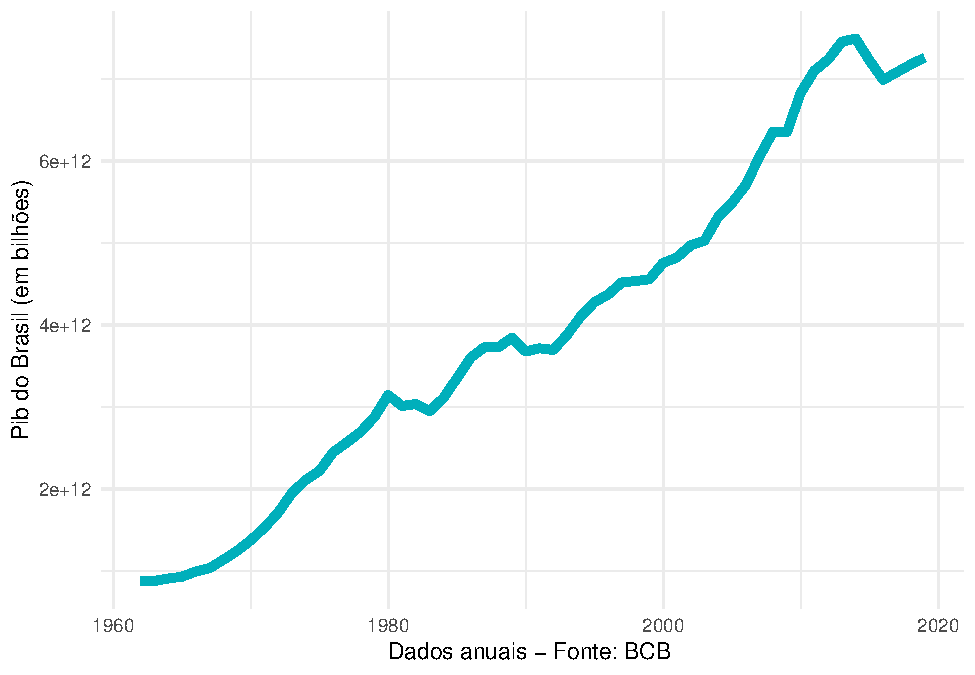
\includegraphics[width=0.45\linewidth]{00-intro_files/figure-latex/tsint00-1} 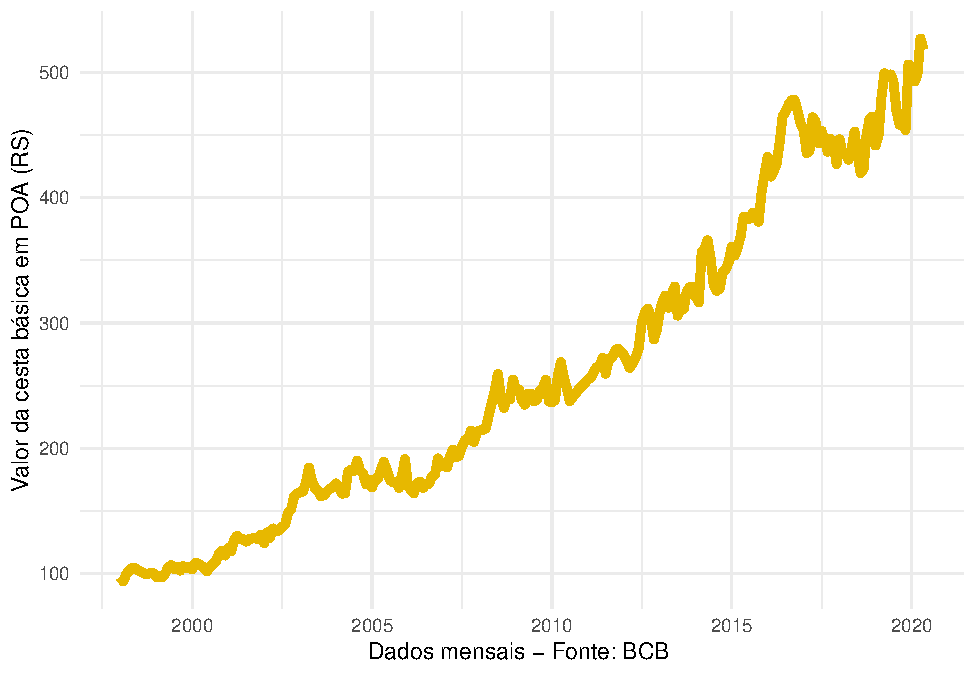
\includegraphics[width=0.45\linewidth]{00-intro_files/figure-latex/tsint00-2} 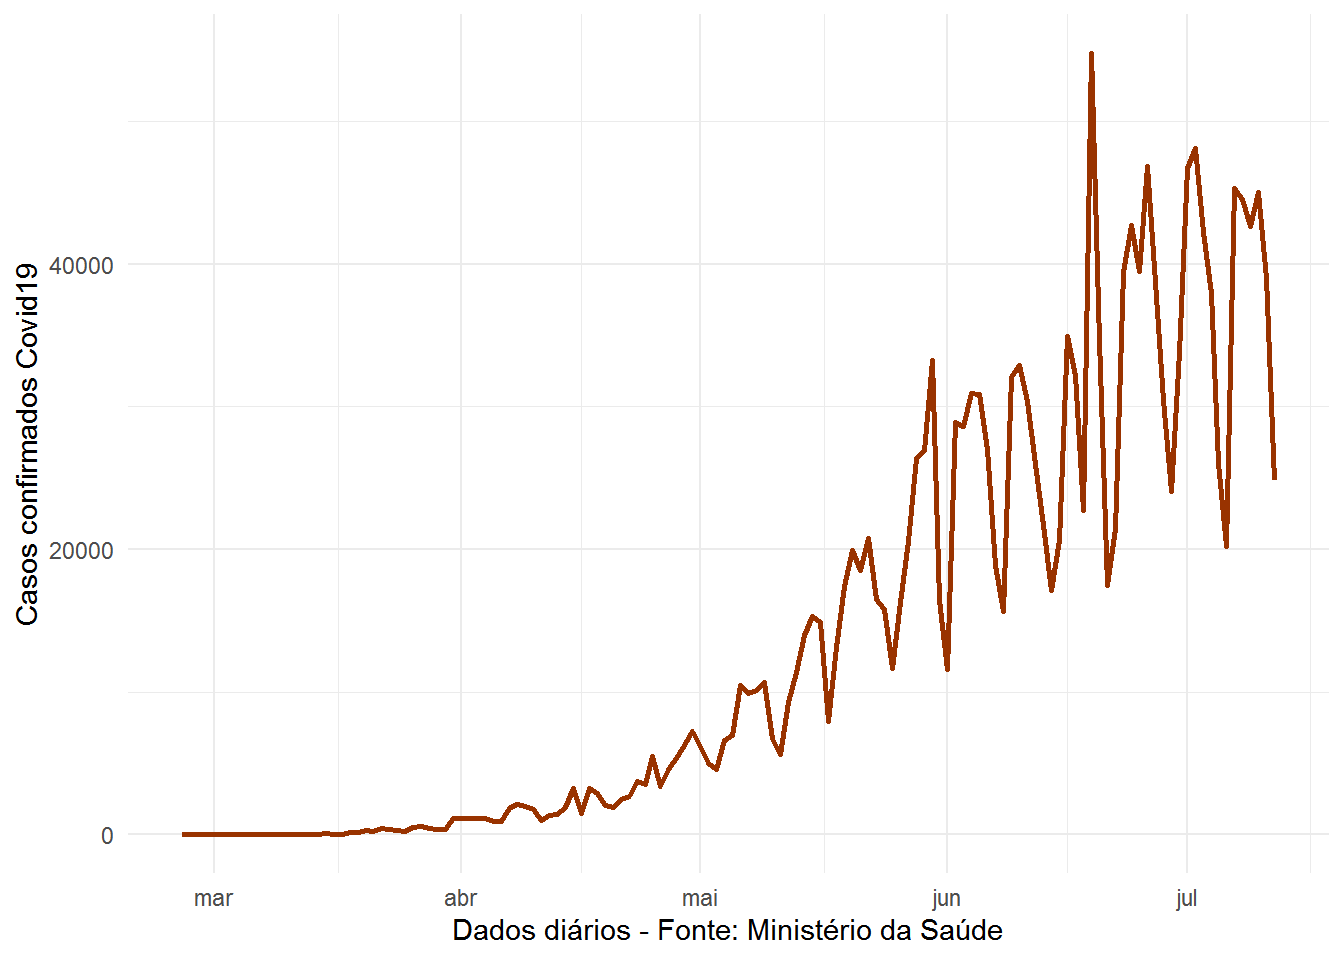
\includegraphics[width=0.45\linewidth]{00-intro_files/figure-latex/tsint00-3} 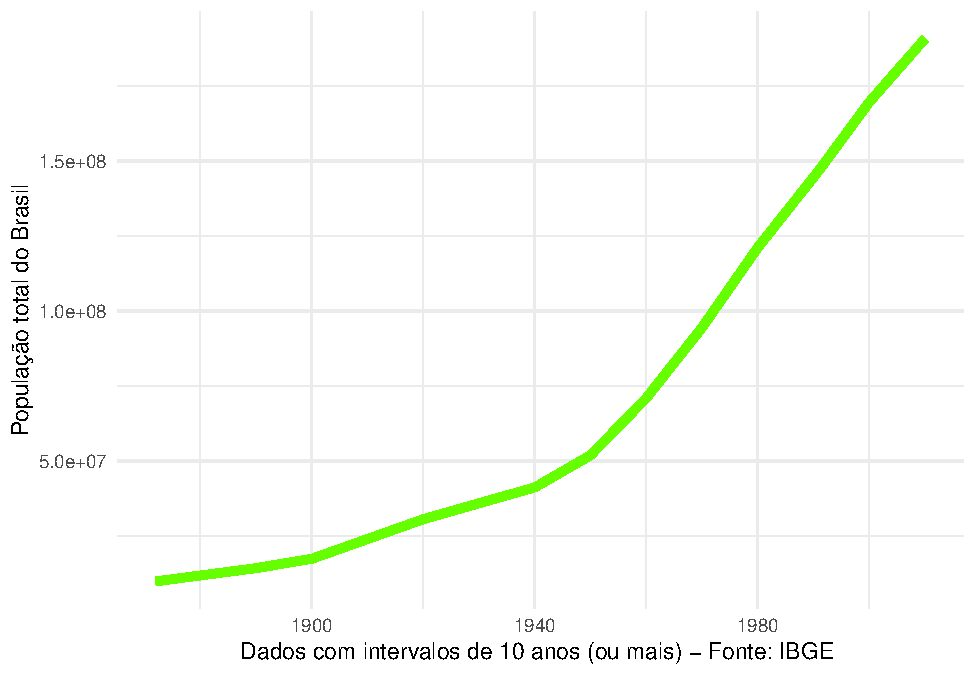
\includegraphics[width=0.45\linewidth]{00-intro_files/figure-latex/tsint00-4} 

}

\caption{Séries temporais com diferentes intervalos de observações}\label{fig:tsint00}
\end{figure}

Uma série temporal com observações a cada dez anos é a da população brasileira.

\hypertarget{intro}{%
\section{Breve introdução ao R}\label{intro}}

Das linguagems de programação voltadas a manipulação, vizualização e análises de dados, o R é umas das mais difundidas entre a comunidade Estatística. Outras linguagens, como o Python, tem um apelo maior quando se trata de ciência de dados, no seu sentido mais amplo.

\hypertarget{apresentauxe7uxe3o-da-linguagem-r}{%
\section{Apresentação da linguagem R}\label{apresentauxe7uxe3o-da-linguagem-r}}

R é uma linguagem de programação caracterizada como Software Livre sob os termos da \emph{General Public License (GNU)} da \emph{Free Software Foundation} no formato \emph{open source}. É voltada a manipulação, análise e vizualização de dados e tem como característica o aspecto colaborativo, sendo que as ferramentas desenvolvidas são compartilhadas online pelos desenvolvedores, podendo ter acesso a elas qualquer pessoa, sem restrições. Uma breve história do R pode ser encontrada no \href{https://pt.wikipedia.org/wiki/R_(linguagem_de_programa\%C3\%A7\%C3\%A3o)}{wikipedia}.

\hypertarget{instalando-o-r}{%
\section{Instalando o R}\label{instalando-o-r}}

Para instalar no computador, O R deve ser baixado do \href{https://cran.r-project.org/}{CRAN}.

\begin{figure}
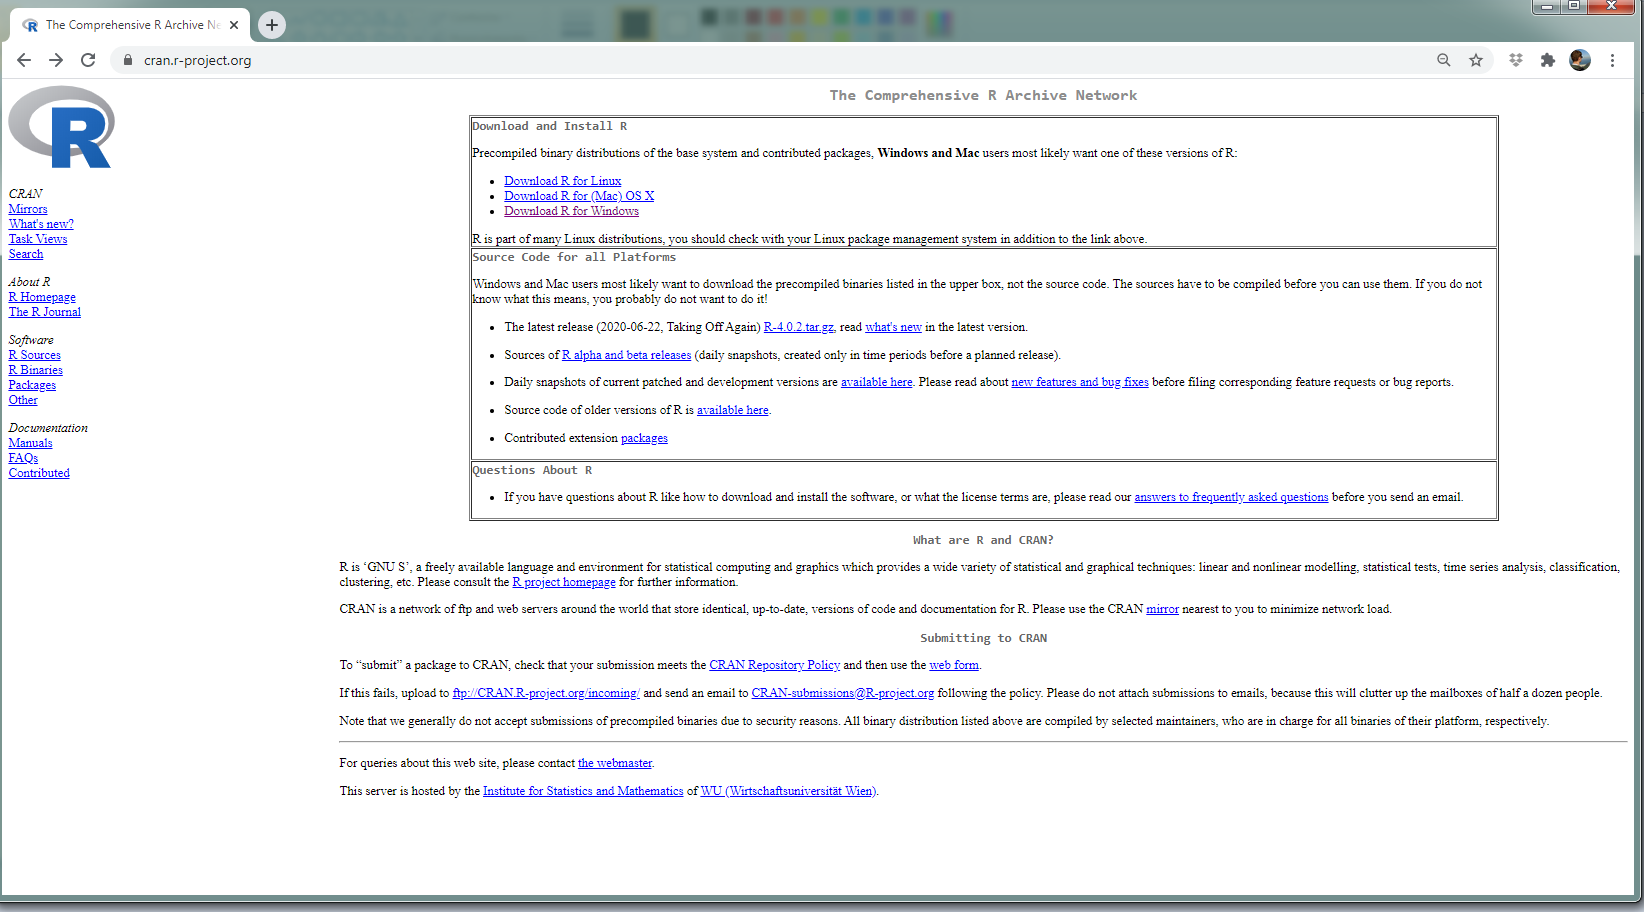
\includegraphics[width=0.9\linewidth]{Figuras/CRAN} \caption{Comprehensive R archive network (CRAN)}\label{fig:cran}
\end{figure}

Se o sistema operacional for Linux, uma versão \emph{base} do R ja vem instalada. No cado de outros sistemas operacionais, como o Windows, é necessário instalar o R \href{https://cran.r-project.org/bin/windows/base/}{base}.

\hypertarget{instalando-o-rstudio}{%
\section{Instalando o RStudio}\label{instalando-o-rstudio}}

Como quase toda linguagem \emph{Open Source} a utilização se dá por meio de linhas de comando. Para tornar a linguagem mais amigável aos usuários, várias IDEs (\emph{integrated development environment}) são utilizadas. No caso do R, a mais desenvolvida e utilizada é o \href{https://rstudio.com/products/rstudio/}{RStudio}.

Uma versão \emph{Free} do RStudio para o seu desktop pode ser baixado de \url{https://rstudio.com/products/rstudio/download/}.

Depois de instalar o R, o RStudio já estará integrado ao R e terá uma interface intuitiva e amigável ao usuário.

\begin{quote}
Ainda assim, é importante ressaltar que na linguagem R não encontraremos \emph{botões} para realizar as análises.
\end{quote}

\begin{figure}
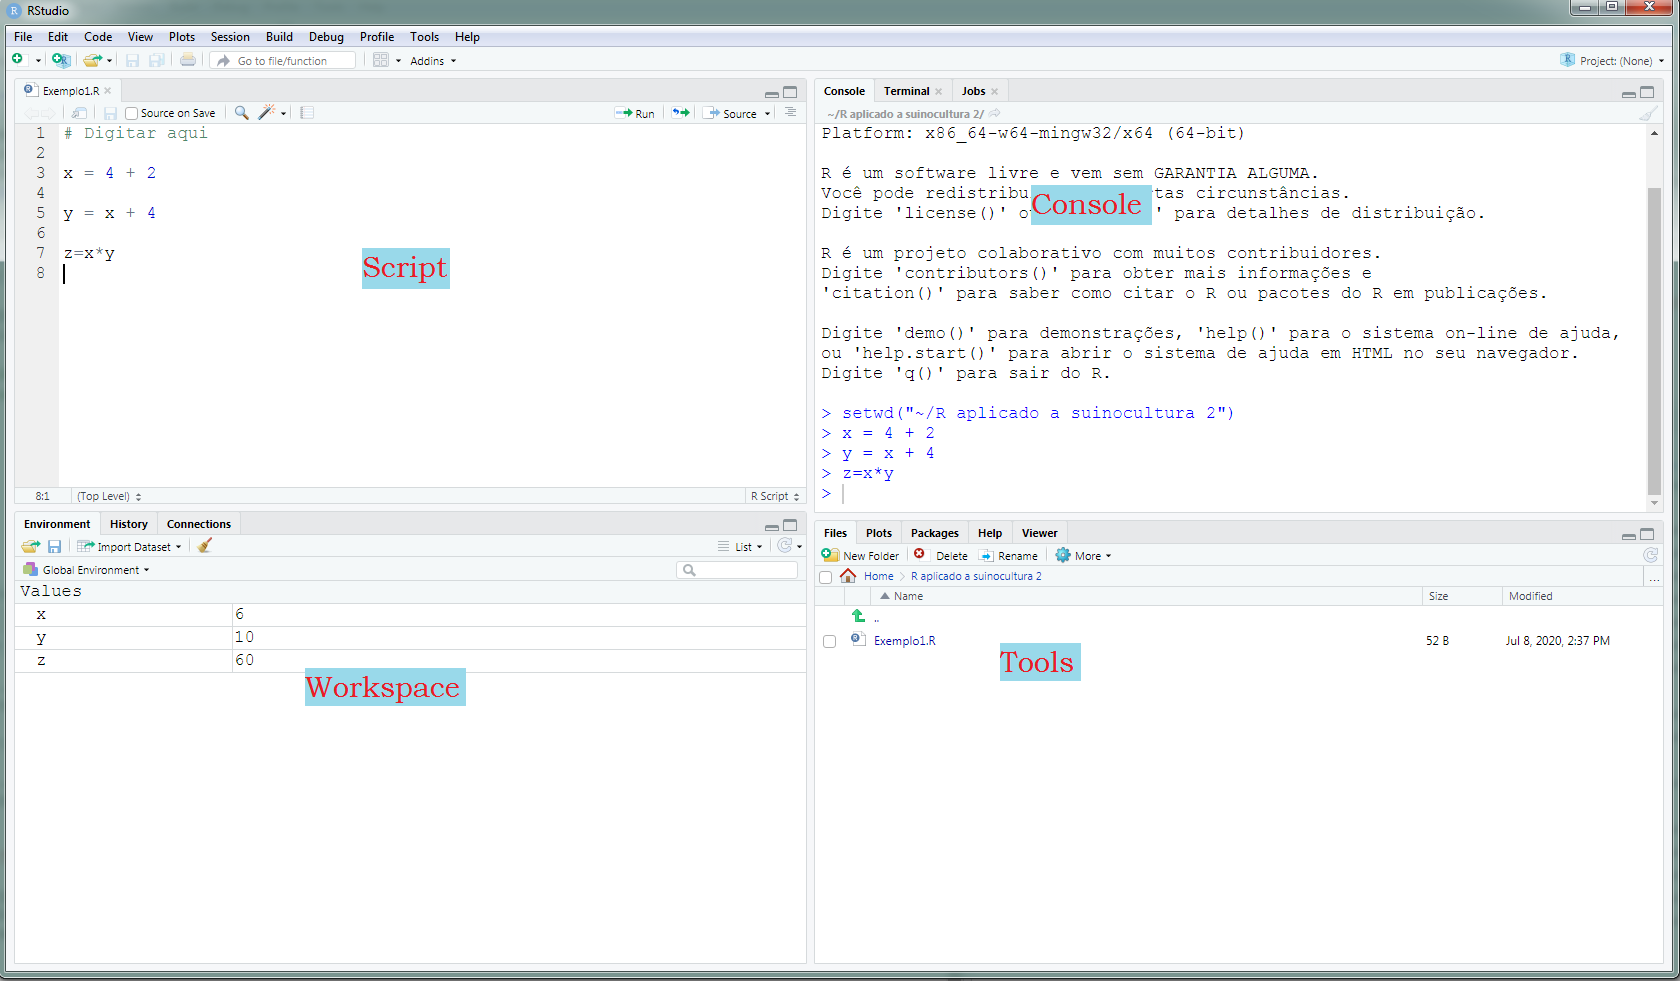
\includegraphics[width=0.9\linewidth]{Figuras/RStudio} \caption{Interface do RStudio}\label{fig:rstudio}
\end{figure}

\hypertarget{diretuxf3rio-de-trabalho}{%
\section{Diretório de trabalho}\label{diretuxf3rio-de-trabalho}}

Um ação importante que deve ser realizada pelo usuário é \emph{setar o diretório} de trabalho. Para isso existem diferentes formas. Uma delas é usando a função \emph{setwd()} .

Outra opção é através do \emph{Go to directory} que está disponível no Workspace do RStudio, conforme figura \ref{fig:rstudio2}. Nessa opção o usuário escolhe o diretório de trabalho e depois usando a opção \emph{set as working directory} esse diretório será ``\emph{settado}'' como diretório de trabalho.

\begin{quote}
Todas os arquivos gerados, como figuras serão salvos nesse diretório. Para abrir um conjunto de dados, por exemplo, será muito mais simples se este também estiver salvo no mesmo diretório ou um subdiretório. Além disso, toda vez que o RStudio for reinicializado, esse procedimento terá que ser refeito.
\end{quote}

\hypertarget{rstudio-cloud}{%
\section{RStudio Cloud}\label{rstudio-cloud}}

Outra forma simples e prática para usar o \texttt{R} e o RStudio é usar o \href{https://rstudio.cloud/}{RStudio Cloud}.

\begin{quote}
\emph{THE MISSION
We created RStudio Cloud to make it easy for professionals, hobbyists, trainers, teachers and students to do, share, teach and learn data science}. \citep{rstudiocloud}
\end{quote}

\begin{figure}

\includegraphics[width=0.9\linewidth]{Figuras/RStudioCloud} \caption{Rstudio Cloud}\label{fig:rstudiocloud}
\end{figure}

Na núvem é possível usar o RStudio utilizando um login através da conta google, ou criar gratuitamente uma conta. Uma vez logado, escolhendo a opção \emph{project} o usuário terá uma versão do RStudio perfeitamente funcional, que pode ser utilizada até no smartphone. Obviamente, é necessário ter conexão com a internet para que a ferramenta possa ser utilizada.

\begin{figure}
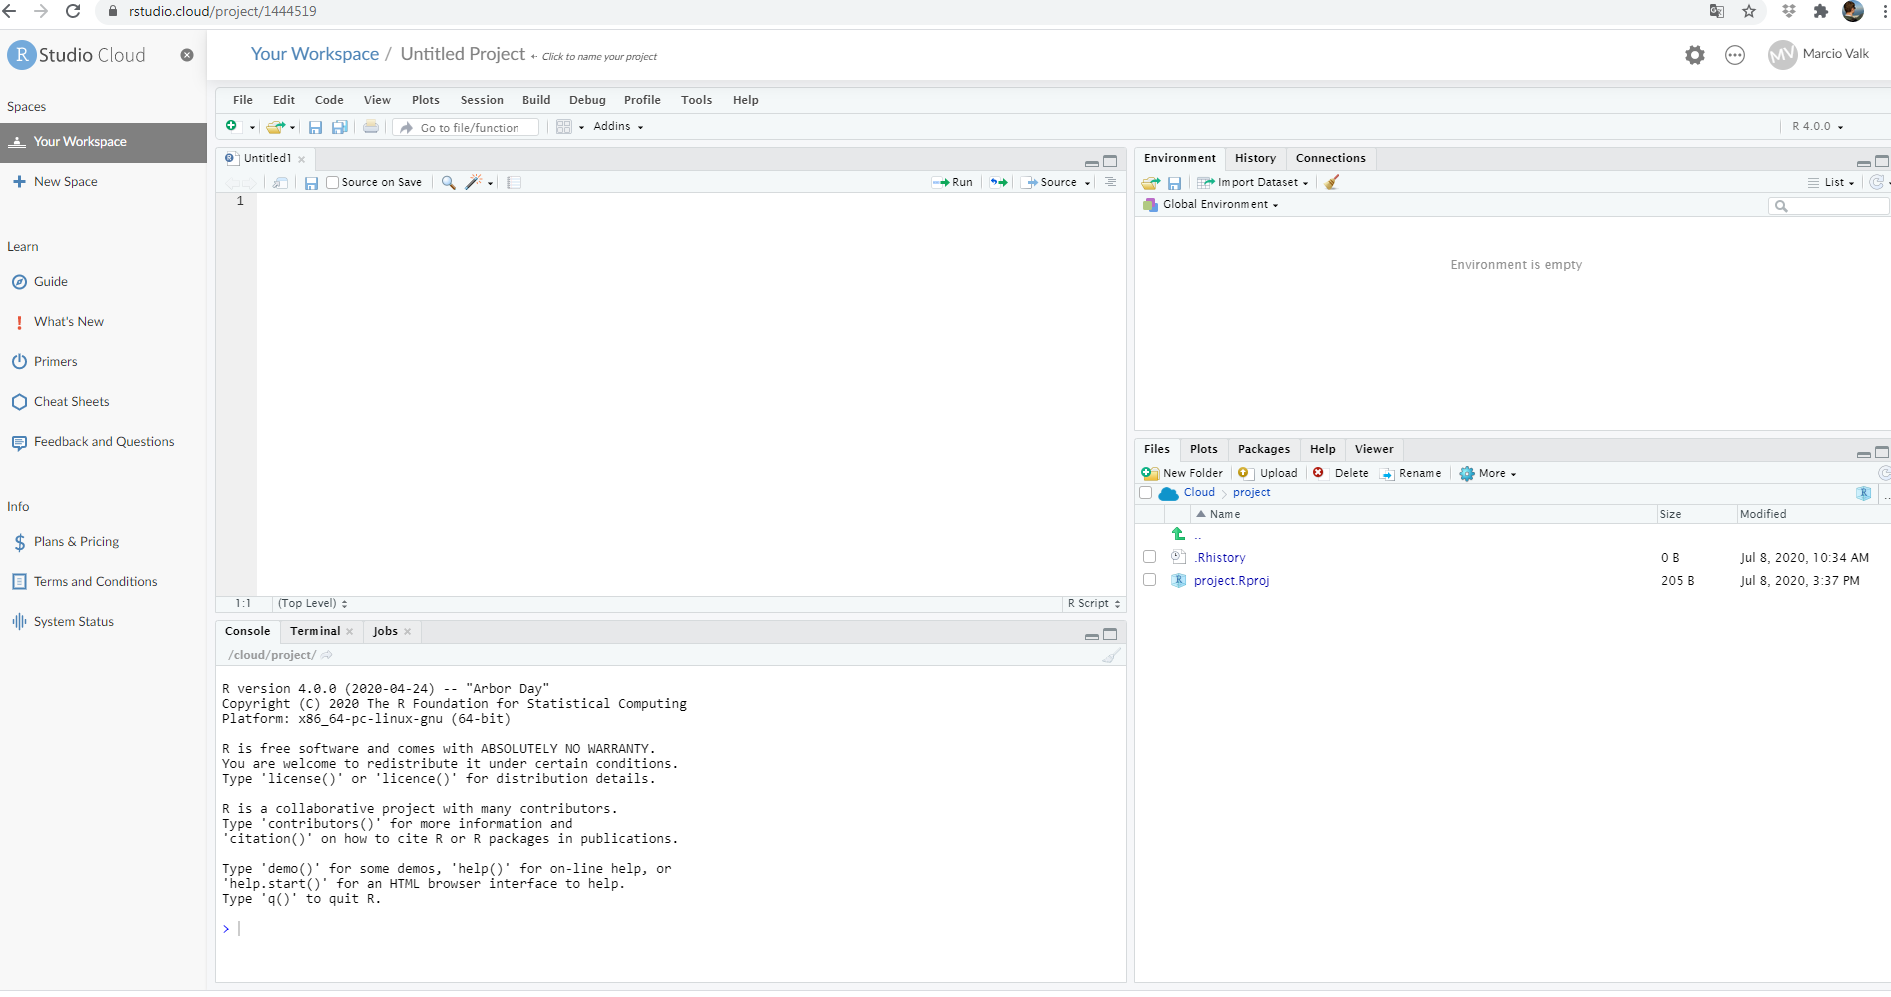
\includegraphics[width=0.9\linewidth]{Figuras/RStudioCloud2} \caption{Rstudio Cloud}\label{fig:rstudiocloud2}
\end{figure}

\hypertarget{instalauxe7uxe3o-de-pacotes}{%
\section{Instalação de pacotes}\label{instalauxe7uxe3o-de-pacotes}}

Na versão \emph{base} do \texttt{R}, uma série de ferramentas, funções e métodos estatísticos são disponibilizados. Além disso, alguns pacotes também compõe a versão \emph{base} do \texttt{R}. Depois de instalado, o usuário pode verificar quais pacotes estão instalados acessando o ícone \emph{Packages} em \emph{Tools} ou digitando \emph{installed.packages()} no \emph{console}.

Para instalar um novo pacote, o usuário pode acessar o ícone \emph{Packages} e depois clicar em \emph{Install} ou digitar no console \emph{install.packages(``nome do pacote'')} . Como exemplo, podemos instalar o pacote usado para vizualização de dados chamado \emph{ggplot2}.

\begin{Shaded}
\begin{Highlighting}[]
\KeywordTok{install.packages}\NormalTok{(}\StringTok{"ggplot2"}\NormalTok{)}
\end{Highlighting}
\end{Shaded}

\hypertarget{carregando-pacotes}{%
\subsection{Carregando pacotes}\label{carregando-pacotes}}

Importante para usuários iniciantes na linguagem \texttt{R} é entender a diferença entre instalar pacotes e carregar pacotes. Uma vez instalado, o pacote estará a disposição do usuário sempre que ele precisar, mas é necessário carregá-lo. É comum deixar um comando nos \emph{scripts} para que cada vez que seja necessário usar alguma função específica de um pacote, ele primeiro seja carregado. O comando usado é o \emph{library()} mas pode ser feito acessando o espaço que chamando de \textbf{Tools}, clicar em \emph{Packages} e marcar o pacote desejado para carregá-lo.

\begin{Shaded}
\begin{Highlighting}[]
\KeywordTok{library}\NormalTok{(ggplot2)}
\end{Highlighting}
\end{Shaded}

\hypertarget{ajuda}{%
\section{Ajuda}\label{ajuda}}

Para um usuário iniciante no \texttt{R} é fundamental saber como resolver problemas diversos que certamente vão surgir durante a instalação de um pacote, uso de uma função, criação de um gráfico, manipulação de dados, etc. Muitas coisas no \texttt{R} são feitas por tentativa e erro, mas o conhecimento é acumulativo e problemas similares, poderão ter uma solução mais rápida. Uma das grandes vantagens da utilização do \texttt{R} é que a comunidade é bastante ativa. Existem diferentes formas de conseguir ajuda e vou elencá-las em ordem de importância, segundo a forma utilização desse autor:

\begin{itemize}
\item
  \begin{quote}
  Google
  \end{quote}
\item
  \begin{quote}
  Stack Overflow
  \end{quote}
\item
  \begin{quote}
  Help do R ( \texttt{help()} ou \texttt{?})
  \end{quote}
\end{itemize}

\hypertarget{google}{%
\subsection{Google}\label{google}}

Para um iniciante em \texttt{R} coisas simples como calcular a raíz quadrada de um número pode ser difícil. Nesses caso o google é muito útil.

\begin{figure}
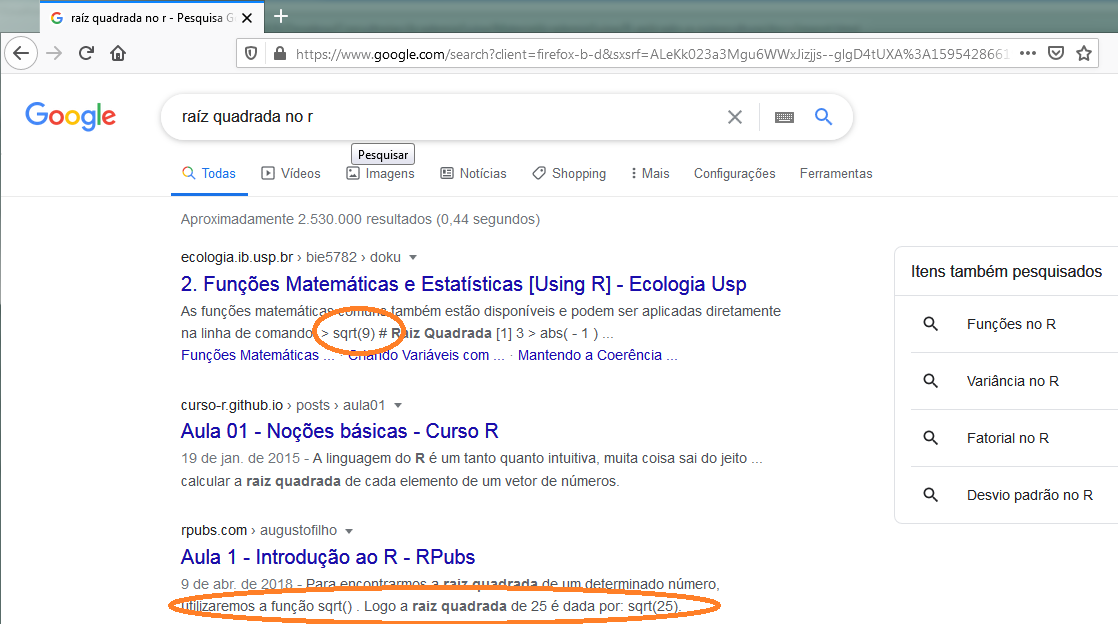
\includegraphics[width=0.9\linewidth]{Figuras/sqrt} \caption{Rstudio Cloud}\label{fig:sq1}
\end{figure}

Um pouco de conhecimento de inglês aumenta consideravelmente as opções de ajuda no google.

\hypertarget{stack-overflow}{%
\subsection{Stack Overflow}\label{stack-overflow}}

Quando o problema parecer um pouco mais complexo, uma opção é colocar a pergunta no google junto com \emph{Stack Overflow}. Isso provavelmente direcionará o usuário para \href{https://pt.stackoverflow.com/}{Stack Overflow em Português} ou \href{https://stackoverflow.com/}{Stack Overflow} que são sites de Pergunta e Resposta utilizados por todas as linguagens de programação.

\begin{figure}
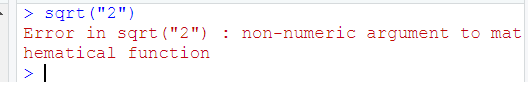
\includegraphics[width=0.9\linewidth]{Figuras/sqrt3} \caption{Rstudio Cloud}\label{fig:sq3}
\end{figure}

\begin{figure}
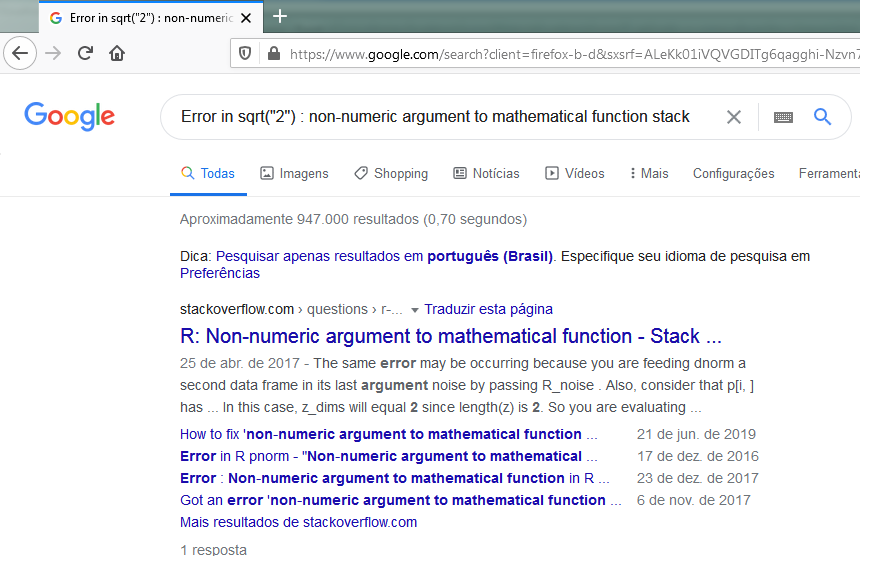
\includegraphics[width=0.9\linewidth]{Figuras/sqrt2} \caption{Rstudio Cloud}\label{fig:sq2}
\end{figure}

\hypertarget{help-do-r}{%
\subsection{\texorpdfstring{Help do \texttt{R}}{Help do R}}\label{help-do-r}}

Se o usuário já sabe qual função deve ser usada, então a documentação do \texttt{R} é bem útil.

\begin{Shaded}
\begin{Highlighting}[]
\NormalTok{?sqrt}
\KeywordTok{help}\NormalTok{(sqrt)}
\end{Highlighting}
\end{Shaded}

Dicas para uso do \texttt{Help}

\begin{itemize}
\tightlist
\item
  Pode-se ir direto aos exemplos que estão no final;
\item
  Identificar os parâmetros (\emph{Arguments});
\item
  Funções relacionadas podem ajudar, dependendo da necessida.
\item
  \emph{Vignettes}, que são tutorias mais completos, mas somente alguns pacotes possuem. Esses textos podem ser acessados com a função vignette(package = `nomeDoPacote'). Por exemplo, vignette(package = `ggplot2')
\end{itemize}

\hypertarget{funcionalidades-buxe1sicas}{%
\section{Funcionalidades básicas}\label{funcionalidades-buxe1sicas}}

Para maior agilidade é importante que o usuário conheça algumas teclas de atalho. Apertando simultaneamente \textbf{\emph{Alt + Shift + K}} o usuário tem acesso à uma grande quantidade de atalhos. Ou clicado em \emph{Tools} no menu de ícones do RStudio.
Um comando de atalho que destacaria por ser extremamaente útil é o \textbf{\emph{Ctrl + Enter}}. Esse comando executa a linha do \emph{script} em que o cursor está.

Para começar, usaremos o \texttt{R} como uma calculadora simples. Execute o código a seguir diretamente do console do RStudio ou no RStudio, escrevendo-os em um script e executando-os usando \textbf{\emph{Ctrl + Enter}}.

\hypertarget{operauxe7uxf5es-buxe1sicas}{%
\subsection{Operações básicas}\label{operauxe7uxf5es-buxe1sicas}}

\hypertarget{as-quatro-operauxe7uxf5es}{%
\subsubsection{As quatro operações}\label{as-quatro-operauxe7uxf5es}}

\begin{longtable}[]{@{}ccc@{}}
\toprule
Operação & código \texttt{R} & Resultado\tabularnewline
\midrule
\endhead
\(3 + 2\) & \texttt{3\ +\ 2} & 5\tabularnewline
\(3 - 2\) & \texttt{3\ -\ 2} & 1\tabularnewline
\(3 \cdot2\) & \texttt{3\ *\ 2} & 6\tabularnewline
\(3 / 2\) & \texttt{3\ /\ 2} & 1.5\tabularnewline
\bottomrule
\end{longtable}

\begin{Shaded}
\begin{Highlighting}[]
\NormalTok{x <-}\StringTok{ }\DecValTok{10}
\NormalTok{y <-}\StringTok{ }\DecValTok{2}

\NormalTok{x}\OperatorTok{+}\NormalTok{y}
\end{Highlighting}
\end{Shaded}

\begin{verbatim}
## [1] 12
\end{verbatim}

\begin{Shaded}
\begin{Highlighting}[]
\NormalTok{x}\OperatorTok{-}\NormalTok{y}
\end{Highlighting}
\end{Shaded}

\begin{verbatim}
## [1] 8
\end{verbatim}

\begin{Shaded}
\begin{Highlighting}[]
\NormalTok{x}\OperatorTok{*}\NormalTok{y}
\end{Highlighting}
\end{Shaded}

\begin{verbatim}
## [1] 20
\end{verbatim}

\begin{Shaded}
\begin{Highlighting}[]
\NormalTok{x}\OperatorTok{/}\NormalTok{y}
\end{Highlighting}
\end{Shaded}

\begin{verbatim}
## [1] 5
\end{verbatim}

\hypertarget{exponenciauxe7uxe3o}{%
\subsubsection{Exponenciação}\label{exponenciauxe7uxe3o}}

\begin{longtable}[]{@{}ccc@{}}
\toprule
Operação & código \texttt{R} & Resultado\tabularnewline
\midrule
\endhead
\(3^2\) & \texttt{3\ \^{}\ 2} & 9\tabularnewline
\(2^{(-3)}\) & \texttt{2\ \^{}\ (-3)} & 0.125\tabularnewline
\(100^{1/2}\) & \texttt{100\ \^{}\ (1\ /\ 2)} & 10\tabularnewline
\(\sqrt{100}\) & \texttt{sqrt(100)} & 10\tabularnewline
\bottomrule
\end{longtable}

\begin{Shaded}
\begin{Highlighting}[]
\NormalTok{x}\OperatorTok{^}\NormalTok{y         }\CommentTok{# x=10 e y=2}
\end{Highlighting}
\end{Shaded}

\begin{verbatim}
## [1] 100
\end{verbatim}

\hypertarget{logaruxedtimos}{%
\subsubsection{Logarítimos}\label{logaruxedtimos}}

Observe que não existe \texttt{ln()} no \texttt{R}. Usa-se \texttt{log()} para significar logarítimo natural. Para as demais bases, é necessário especificar a base desejada.

\begin{longtable}[]{@{}ccc@{}}
\toprule
Operação & código \texttt{R} & Resultado\tabularnewline
\midrule
\endhead
\(\log(e)\) & \texttt{log(exp(1))} & 1\tabularnewline
\(\log_{10}(100)\) & \texttt{log10(100)} & 2\tabularnewline
\(\log_{2}(16)\) & \texttt{log2(16)} & 4\tabularnewline
\(\log_{4}(16)\) & \texttt{log(16,\ base\ =\ 4)} & 2\tabularnewline
\bottomrule
\end{longtable}

\begin{Shaded}
\begin{Highlighting}[]
\KeywordTok{log}\NormalTok{(x)        }\CommentTok{# x=10}
\end{Highlighting}
\end{Shaded}

\begin{verbatim}
## [1] 2.302585
\end{verbatim}

\begin{Shaded}
\begin{Highlighting}[]
\KeywordTok{log}\NormalTok{(x,}\DataTypeTok{base=}\NormalTok{y) }\CommentTok{# y=2}
\end{Highlighting}
\end{Shaded}

\begin{verbatim}
## [1] 3.321928
\end{verbatim}

\hypertarget{constantes-matemuxe1ticas}{%
\subsubsection{Constantes matemáticas}\label{constantes-matemuxe1ticas}}

\begin{longtable}[]{@{}ccc@{}}
\toprule
Constante & código \texttt{R} & Resultado\tabularnewline
\midrule
\endhead
\(\pi\) & \texttt{pi} & 3.1415927\tabularnewline
\(e\) & \texttt{exp(1)} & 2.7182818\tabularnewline
\bottomrule
\end{longtable}

\begin{Shaded}
\begin{Highlighting}[]
\KeywordTok{log}\NormalTok{(}\KeywordTok{exp}\NormalTok{(}\DecValTok{1}\NormalTok{)) }
\end{Highlighting}
\end{Shaded}

\begin{verbatim}
## [1] 1
\end{verbatim}

\begin{Shaded}
\begin{Highlighting}[]
\KeywordTok{exp}\NormalTok{(}\DecValTok{1}\NormalTok{)}\OperatorTok{^}\NormalTok{y     }\CommentTok{# y=2}
\end{Highlighting}
\end{Shaded}

\begin{verbatim}
## [1] 7.389056
\end{verbatim}

\hypertarget{operadores-luxf3gicos}{%
\subsection{Operadores lógicos}\label{operadores-luxf3gicos}}

\begin{longtable}[]{@{}lccc@{}}
\toprule
Operador & Significado & Exemplo & Resultado\tabularnewline
\midrule
\endhead
\texttt{x\ \textless{}\ y} & \texttt{x} menor do que \texttt{y} & \texttt{3\ \textless{}\ 42} & TRUE\tabularnewline
\texttt{x\ \textgreater{}\ y} & \texttt{x} maior do que \texttt{y} & \texttt{3\ \textgreater{}\ 42} & FALSE\tabularnewline
\texttt{x\ \textless{}=\ y} & \texttt{x} menor ou igual à \texttt{y} & \texttt{3\ \textless{}=\ 42} & TRUE\tabularnewline
\texttt{x\ \textgreater{}=\ y} & \texttt{x} menor ou igual à\texttt{y} & \texttt{3\ \textgreater{}=\ 42} & FALSE\tabularnewline
\texttt{x\ ==\ y} & \texttt{x} igual à \texttt{y} & \texttt{3\ ==\ 42} & FALSE\tabularnewline
\texttt{x\ !=\ y} & \texttt{x} diferente de \texttt{y} & \texttt{3\ !=\ 42} & TRUE\tabularnewline
\texttt{!x} & não \texttt{x} & \texttt{!(3\ \textgreater{}\ 42)} & TRUE\tabularnewline
\texttt{x\ \textbar{}\ y} & \texttt{x} ou \texttt{y} & \texttt{(3\ \textgreater{}\ 42)\ \textbar{}\ TRUE} & TRUE\tabularnewline
\texttt{x\ \&\ y} & \texttt{x} e \texttt{y} & \texttt{(3\ \textless{}\ 4)\ \&\ (\ 42\ \textgreater{}\ 13)} & TRUE\tabularnewline
\bottomrule
\end{longtable}

\hypertarget{operador-luxf3gico-if}{%
\subsubsection{\texorpdfstring{Operador lógico \emph{if()}}{Operador lógico if()}}\label{operador-luxf3gico-if}}

Dentro dessa classe de operadores, podemos destacar o operador \emph{if()}. É comum usar esse operador para testar condições únicas ou múltiplas na instrução \emph{if()} ou \emph{ifelse()}. Operadores lógicos em \texttt{R} podem ser aplicados a vetores numéricos ou complexos ou objetos booleanos, que são \textbf{TRUE} ou \textbf{FALSE} (à eles são reservados os \emph{atalhos} \textbf{T} e \textbf{F}).

\begin{Shaded}
\begin{Highlighting}[]
\NormalTok{A=}\DecValTok{4}
\NormalTok{B=}\DecValTok{2}
\ControlFlowTok{if}\NormalTok{(A}\OperatorTok{>}\NormalTok{B)\{}
  \KeywordTok{print}\NormalTok{(}\StringTok{"A é maior do que B"}\NormalTok{)}
\NormalTok{  \}}\ControlFlowTok{else}\NormalTok{\{}
    \KeywordTok{print}\NormalTok{(}\StringTok{"A não é maior do que B"}\NormalTok{)}
\NormalTok{  \}}
\end{Highlighting}
\end{Shaded}

\begin{verbatim}
## [1] "A é maior do que B"
\end{verbatim}

\begin{Shaded}
\begin{Highlighting}[]
\NormalTok{A=}\DecValTok{4}
\NormalTok{B=}\DecValTok{6}
\ControlFlowTok{if}\NormalTok{(A}\OperatorTok{>}\NormalTok{B)\{}
  \KeywordTok{print}\NormalTok{(}\StringTok{"A é maior do que B"}\NormalTok{)}
\NormalTok{  \}}\ControlFlowTok{else}\NormalTok{\{}
    \KeywordTok{print}\NormalTok{(}\StringTok{"A não é maior do que B"}\NormalTok{)}
\NormalTok{  \}}
\end{Highlighting}
\end{Shaded}

\begin{verbatim}
## [1] "A não é maior do que B"
\end{verbatim}

Outra forma simples de usar o operador é:

\begin{Shaded}
\begin{Highlighting}[]
\NormalTok{A=}\DecValTok{4}
\NormalTok{B=}\DecValTok{6}
\NormalTok{A}\OperatorTok{>}\NormalTok{B}
\end{Highlighting}
\end{Shaded}

\begin{verbatim}
## [1] FALSE
\end{verbatim}

\hypertarget{operador-luxf3gico-ifelse}{%
\subsubsection{\texorpdfstring{Operador lógico \emph{ifelse()}}{Operador lógico ifelse()}}\label{operador-luxf3gico-ifelse}}

O operador \emph{ifelse( ``1'', ``2'' , ``3'')} possui 3 entradas. Na primeira ``1'', deve-se colocar a condição a ser testada. Em ``2'' o resultado caso a condição testada seja verdadeira e em ``3'' o resultado, caso a condição testada seja falsa.

\begin{Shaded}
\begin{Highlighting}[]
\NormalTok{A=}\DecValTok{4}
\NormalTok{B=}\DecValTok{6}
\CommentTok{#ifelse(A>=B,"Verdadeiro","FALSO")}
\end{Highlighting}
\end{Shaded}

\hypertarget{operadores-de-atribuiuxe7uxe3o}{%
\subsubsection{Operadores de atribuição}\label{operadores-de-atribuiuxe7uxe3o}}

Os operadores de atribuição são provavelmente a família de operadores que você mais usará enquanto
trabalha com \texttt{R}. Como o nome desse grupo implica, eles são usados para atribuir objetos, como
valores numéricos, \emph{strings}, vetores, modelos e plotagens para um nome (variável). Isso inclui
operadores como a seta para trás (\textless-) ou o sinal de igual (=)

\begin{Shaded}
\begin{Highlighting}[]
\NormalTok{str <-}\StringTok{ "Em Brasília, 19 horas!"} \CommentTok{# String}
\NormalTok{int <-}\StringTok{ }\DecValTok{10} \CommentTok{# Inteiro}
\NormalTok{vet <-}\StringTok{ }\KeywordTok{c}\NormalTok{(}\DecValTok{1}\NormalTok{,}\DecValTok{2}\NormalTok{,}\DecValTok{3}\NormalTok{,}\DecValTok{4}\NormalTok{) }\CommentTok{# Vetor}
\end{Highlighting}
\end{Shaded}

Para visualizar a variável, podemos simplesmente digitá-la ou usar a função \emph{print()}

\begin{Shaded}
\begin{Highlighting}[]
\NormalTok{str}
\end{Highlighting}
\end{Shaded}

\begin{verbatim}
## [1] "Em Brasília, 19 horas!"
\end{verbatim}

\begin{Shaded}
\begin{Highlighting}[]
\CommentTok{#ou}
\KeywordTok{print}\NormalTok{(str)}
\end{Highlighting}
\end{Shaded}

\begin{verbatim}
## [1] "Em Brasília, 19 horas!"
\end{verbatim}

Para visualizar mais de uma variável, podemos usar ``c()'' para ``juntar as variáveis''

\begin{Shaded}
\begin{Highlighting}[]
\KeywordTok{c}\NormalTok{(str,int)}
\end{Highlighting}
\end{Shaded}

\begin{verbatim}
## [1] "Em Brasília, 19 horas!" "10"
\end{verbatim}

\begin{Shaded}
\begin{Highlighting}[]
\CommentTok{# ou}
\KeywordTok{print}\NormalTok{(}\KeywordTok{c}\NormalTok{(str,int))}
\end{Highlighting}
\end{Shaded}

\begin{verbatim}
## [1] "Em Brasília, 19 horas!" "10"
\end{verbatim}

\begin{quote}
\emph{Esse exemplo pode ser repetido usando ``='' no lugar de ``\textless-''}
\end{quote}

\hypertarget{tipos-de-dados}{%
\subsection{Tipos de dados}\label{tipos-de-dados}}

\texttt{R} possui um número básico de \emph{tipos} de dados. Enquanto o \texttt{R}é uma \emph{linguagem fortemente tipada} (não exige do usuário muito conhecimento sobre diferentes tipos de dados) é útil conhecer os tipos disponíveis.

\begin{itemize}
\tightlist
\item
  Numeric

  \begin{itemize}
  \tightlist
  \item
    Também conhecido como duplo. O tipo padrão ao lidar com números.
  \item
    Exemplos: \texttt{1},\texttt{1,0}, \texttt{42,5}
  \end{itemize}
\item
  Integer

  \begin{itemize}
  \tightlist
  \item
    Exemplos: \texttt{1L},\texttt{2L}, \texttt{42L}
  \end{itemize}
\item
  Complex

  \begin{itemize}
  \tightlist
  \item
    Exemplo: \texttt{4\ +\ 2i}
  \end{itemize}
\item
  Logical

  \begin{itemize}
  \tightlist
  \item
    Dois valores possíveis: \texttt{TRUE} e \texttt{FALSE}
  \item
    Você também pode usar \texttt{T} e\texttt{F}, mas isso \emph{não} é recomendado.
  \item
    \texttt{NA} também é considerado lógico.
  \end{itemize}
\item
  Character

  \begin{itemize}
  \tightlist
  \item
    Exemplos: \texttt{"\ a\ "}, \texttt{"\ Statistics\ "}, \texttt{"\ 1\ mais\ 2.\ "}
  \end{itemize}
\item
  Categorical or \texttt{factor}

  \begin{itemize}
  \tightlist
  \item
    Uma mistura de número inteiro e caractere. Uma variável \texttt{fator} atribui um rótulo a um valor numérico.
  \item
    Por exemplo, \texttt{fator\ (x\ =\ c\ (0,1),\ labels\ =\ c\ ("\ male\ ","\ female\ ")))} atribui a string \emph{male} aos valores numéricos \texttt{0} e a string \emph{female} ao valor \texttt{1}.
  \end{itemize}
\end{itemize}

\hypertarget{valores-especiais}{%
\subsection{Valores especiais}\label{valores-especiais}}

Assim como \texttt{TRUE} e \texttt{FALSE}, existem outros \emph{valores} reservados à situações específicas.

\begin{itemize}
\tightlist
\item
  \texttt{NA} (\emph{Not Available}) representa dado faltante (não disponível), ou que que é chamado em estatística de \emph{missing data}.
\item
  \texttt{NaN} (\emph{Not a Number}) são gerados quando temos uma indefinições matemáticas, como sqrt(-1) e 0/0.
\item
  \texttt{Inf} (\emph{Infinito}) é usado quando o valor numérico é muito grande (limite). Por exemplo, \texttt{exp(2000)}.
\item
  \texttt{NULL} significa ausência de informação. Parecido com o \texttt{NA}, mas conceitualmente mais usado na lógica de programação.
\end{itemize}

As funções \texttt{is.na()}, \texttt{is.nan()}, \texttt{is.infinite()} e \texttt{is.null()}podem ser usadas para verificar se um objeto possui algum valor com essa caraterística.

\hypertarget{estrutura-dos-dados}{%
\section{Estrutura dos dados}\label{estrutura-dos-dados}}

\texttt{R} também possui um número básico de \emph{estrutura} de dados. Essa estrutura de dados pode ser \textbf{homogênea} ( setodos os elementos são do mesmo tipo de dados) ou \textbf{heterogênea} (se os elementos podem ter mais de um tipo de dados).

\begin{longtable}[]{@{}ccc@{}}
\toprule
Dimensão & \textbf{Homogênea} & \textbf{Heterogênea}\tabularnewline
\midrule
\endhead
1 & Vector & List\tabularnewline
2 & Matrix & Data Frame\tabularnewline
3+ & Array & nested Lists\tabularnewline
\bottomrule
\end{longtable}

\hypertarget{vetores}{%
\subsection{Vetores}\label{vetores}}

Muitas operações em \texttt{R} usam \textbf{vetores}. Um vetor contém um conjunto de objetos de tipos identicos e são indexados começando na posição \texttt{1}. A maneira mais comum para se criar um vetor é usar a função \texttt{c()}, o que é uma abreviação de \texttt{combine()}. Ela combina uma lista de elementos separados por \texttt{,}. Por exemplo,

\begin{Shaded}
\begin{Highlighting}[]
\KeywordTok{c}\NormalTok{(}\DecValTok{1}\NormalTok{,}\DecValTok{2}\NormalTok{)}
\end{Highlighting}
\end{Shaded}

\begin{verbatim}
## [1] 1 2
\end{verbatim}

Ou podemos combinar outros objetos, desde que sejam do mesmo tipo.

\begin{Shaded}
\begin{Highlighting}[]
\NormalTok{A=}\KeywordTok{c}\NormalTok{(}\DecValTok{1}\NormalTok{,}\DecValTok{2}\NormalTok{)}
\NormalTok{B=}\KeywordTok{c}\NormalTok{(}\DecValTok{3}\NormalTok{,}\DecValTok{4}\NormalTok{,}\DecValTok{5}\NormalTok{)}
\KeywordTok{c}\NormalTok{(A,B)}
\end{Highlighting}
\end{Shaded}

\begin{verbatim}
## [1] 1 2 3 4 5
\end{verbatim}

Os objetos não precisam ser numéricos. Por exemplo,

\begin{Shaded}
\begin{Highlighting}[]
\NormalTok{A=}\StringTok{"Amarelo"}  \CommentTok{# objeto da classe "character"}
\KeywordTok{class}\NormalTok{(A)}
\end{Highlighting}
\end{Shaded}

\begin{verbatim}
## [1] "character"
\end{verbatim}

\begin{Shaded}
\begin{Highlighting}[]
\NormalTok{B=}\StringTok{"Azul"}
\KeywordTok{c}\NormalTok{(A,B)}
\end{Highlighting}
\end{Shaded}

\begin{verbatim}
## [1] "Amarelo" "Azul"
\end{verbatim}

Embora tenham muitas \texttt{letras} nesse objeto combinado \texttt{c(A,B)}, na verdade só existem dois elementos, \{``Amarelo'', ``Azul''\}. Para acessá-los, usamos o colchete \texttt{{[}{]}}.

\hypertarget{subconjuntos-de-vetores}{%
\subsubsection{Subconjuntos de vetores}\label{subconjuntos-de-vetores}}

Para subconjunto de um vetor, ou seja, para escolher apenas alguns elementos dele, usamos colchetes, \texttt{{[}{]}}. Aqui vemos que \texttt{AA{[}1{]}} retorna o primeiro elemento e \texttt{AA{[}2{]}} retorna o segundo elemento:

\begin{Shaded}
\begin{Highlighting}[]
\NormalTok{A=}\StringTok{"Amarelo"}
\NormalTok{B=}\StringTok{"Azul"}
\NormalTok{AA=}\KeywordTok{c}\NormalTok{(A,B)}
\NormalTok{AA[}\DecValTok{1}\NormalTok{]}
\end{Highlighting}
\end{Shaded}

\begin{verbatim}
## [1] "Amarelo"
\end{verbatim}

\begin{Shaded}
\begin{Highlighting}[]
\NormalTok{AA[}\DecValTok{2}\NormalTok{]}
\end{Highlighting}
\end{Shaded}

\begin{verbatim}
## [1] "Azul"
\end{verbatim}

Qunado o vetor é maior, podemso usar um conjunto de indices para acessar o valores correspondentes no vetor.

\begin{Shaded}
\begin{Highlighting}[]
\NormalTok{x=}\KeywordTok{c}\NormalTok{(}\DecValTok{35}\NormalTok{,}\DecValTok{42}\NormalTok{,}\DecValTok{47}\NormalTok{,}\DecValTok{54}\NormalTok{,}\DecValTok{70}\NormalTok{,}\DecValTok{75}\NormalTok{)}
\NormalTok{x[}\KeywordTok{c}\NormalTok{(}\DecValTok{1}\NormalTok{,}\DecValTok{3}\NormalTok{,}\DecValTok{6}\NormalTok{)]     }\CommentTok{# Acessa as posições 1, 3 e 6 do vetor}
\end{Highlighting}
\end{Shaded}

\begin{verbatim}
## [1] 35 47 75
\end{verbatim}

\begin{Shaded}
\begin{Highlighting}[]
\NormalTok{x[}\OperatorTok{-}\DecValTok{4}\NormalTok{]           }\CommentTok{# Acessa todas as posições do vetor, menos a posição 4}
\end{Highlighting}
\end{Shaded}

\begin{verbatim}
## [1] 35 42 47 70 75
\end{verbatim}

Muitas vezes queremos criar um vetor baseado em uma sequência de números. No \texttt{R} o operador \texttt{:} é usado como uma opção \texttt{de\ :\ até}. Dessa forma é possível usá-lo em diferentes situações.

\begin{Shaded}
\begin{Highlighting}[]
\KeywordTok{c}\NormalTok{(}\DecValTok{1}\OperatorTok{:}\DecValTok{10}\NormalTok{) }\CommentTok{# vetor com números de 1 à 10}
\end{Highlighting}
\end{Shaded}

\begin{verbatim}
##  [1]  1  2  3  4  5  6  7  8  9 10
\end{verbatim}

\begin{Shaded}
\begin{Highlighting}[]
\DecValTok{1}\OperatorTok{:}\DecValTok{10}    \CommentTok{# vetor com números de 1 à 10}
\end{Highlighting}
\end{Shaded}

\begin{verbatim}
##  [1]  1  2  3  4  5  6  7  8  9 10
\end{verbatim}

Outros vetores de objetos são possíveis de criar

\begin{Shaded}
\begin{Highlighting}[]
\NormalTok{LETTERS[}\DecValTok{1}\OperatorTok{:}\DecValTok{4}\NormalTok{] }\CommentTok{# maiúsculas}
\end{Highlighting}
\end{Shaded}

\begin{verbatim}
## [1] "A" "B" "C" "D"
\end{verbatim}

\begin{Shaded}
\begin{Highlighting}[]
\NormalTok{letters[}\DecValTok{1}\OperatorTok{:}\DecValTok{4}\NormalTok{] }\CommentTok{# minuscúlas}
\end{Highlighting}
\end{Shaded}

\begin{verbatim}
## [1] "a" "b" "c" "d"
\end{verbatim}

\hypertarget{funuxe7uxe3o-paste}{%
\subsubsection{\texorpdfstring{Função \texttt{paste()}}{Função paste()}}\label{funuxe7uxe3o-paste}}

Com a função \texttt{paste()} podemos concatenar objetos de tipos diferentes e armazená-los em um vetor.

\begin{Shaded}
\begin{Highlighting}[]
\KeywordTok{paste}\NormalTok{(}\StringTok{"Porco_"}\NormalTok{, letters[}\DecValTok{1}\OperatorTok{:}\DecValTok{4}\NormalTok{], }\DataTypeTok{sep=}\StringTok{""}\NormalTok{)   }\CommentTok{# Underline no Porco e sem espaço no sep}
\end{Highlighting}
\end{Shaded}

\begin{verbatim}
## [1] "Porco_a" "Porco_b" "Porco_c" "Porco_d"
\end{verbatim}

\begin{Shaded}
\begin{Highlighting}[]
\KeywordTok{paste}\NormalTok{(}\StringTok{"Porco"}\NormalTok{, letters[}\DecValTok{1}\OperatorTok{:}\DecValTok{4}\NormalTok{], }\DataTypeTok{sep=}\StringTok{"_"}\NormalTok{)   }\CommentTok{# Underline no sep}
\end{Highlighting}
\end{Shaded}

\begin{verbatim}
## [1] "Porco_a" "Porco_b" "Porco_c" "Porco_d"
\end{verbatim}

\begin{Shaded}
\begin{Highlighting}[]
\NormalTok{p=}\KeywordTok{paste}\NormalTok{(}\StringTok{"Porco"}\NormalTok{, letters[}\DecValTok{1}\OperatorTok{:}\DecValTok{4}\NormalTok{], }\DataTypeTok{sep=}\StringTok{"_"}\NormalTok{) }\CommentTok{# Armazenando no vetor p}
\NormalTok{p[}\DecValTok{2}\NormalTok{]                                    }\CommentTok{# Acessando a posição 2 do vetor p}
\end{Highlighting}
\end{Shaded}

\begin{verbatim}
## [1] "Porco_b"
\end{verbatim}

Note que escalares não existem no \texttt{R}. Eles são vetores de tamanho \texttt{1}.

\begin{Shaded}
\begin{Highlighting}[]
\DecValTok{2}
\end{Highlighting}
\end{Shaded}

\begin{verbatim}
## [1] 2
\end{verbatim}

\hypertarget{funuxe7uxe3o-seq}{%
\subsubsection{\texorpdfstring{Função \texttt{seq()}}{Função seq()}}\label{funuxe7uxe3o-seq}}

Se quisermos criar uma sequência que não se limite a números inteiros e que aumente 1 por vez, podemos usar a função \texttt{seq()}.

\begin{Shaded}
\begin{Highlighting}[]
\KeywordTok{seq}\NormalTok{(}\DataTypeTok{from =} \FloatTok{-0.5}\NormalTok{, }\DataTypeTok{to =} \FloatTok{1.8}\NormalTok{, }\DataTypeTok{by =} \FloatTok{0.1}\NormalTok{)}
\end{Highlighting}
\end{Shaded}

\begin{verbatim}
##  [1] -0.5 -0.4 -0.3 -0.2 -0.1  0.0  0.1  0.2  0.3  0.4  0.5  0.6  0.7  0.8  0.9
## [16]  1.0  1.1  1.2  1.3  1.4  1.5  1.6  1.7  1.8
\end{verbatim}

\hypertarget{funuxe7uxe3o-rep}{%
\subsubsection{\texorpdfstring{Função \texttt{rep()}}{Função rep()}}\label{funuxe7uxe3o-rep}}

Outra operação comum para criar um vetor é \texttt{rep()}, que pode repetir um único valor várias vezes.

\begin{Shaded}
\begin{Highlighting}[]
\KeywordTok{rep}\NormalTok{(}\StringTok{"A"}\NormalTok{, }\DataTypeTok{times =} \DecValTok{10}\NormalTok{)}
\end{Highlighting}
\end{Shaded}

\begin{verbatim}
##  [1] "A" "A" "A" "A" "A" "A" "A" "A" "A" "A"
\end{verbatim}

\begin{Shaded}
\begin{Highlighting}[]
\KeywordTok{rep}\NormalTok{(}\DecValTok{1}\NormalTok{, }\DecValTok{10}\NormalTok{)}
\end{Highlighting}
\end{Shaded}

\begin{verbatim}
##  [1] 1 1 1 1 1 1 1 1 1 1
\end{verbatim}

A função \texttt{rep()} pode ser usada para repetir um vetor várias vezes.

\begin{Shaded}
\begin{Highlighting}[]
\NormalTok{x=}\KeywordTok{c}\NormalTok{(}\StringTok{"O"}\NormalTok{,}\StringTok{"A"}\NormalTok{)}
\KeywordTok{rep}\NormalTok{(x, }\DecValTok{3}\NormalTok{)}
\end{Highlighting}
\end{Shaded}

\begin{verbatim}
## [1] "O" "A" "O" "A" "O" "A"
\end{verbatim}

\hypertarget{funuxe7uxe3o-length}{%
\subsubsection{\texorpdfstring{Função \texttt{length()}}{Função length()}}\label{funuxe7uxe3o-length}}

Uma função importante é à que identifica o tamanho do vetor, que é a função \texttt{length()}.

\begin{Shaded}
\begin{Highlighting}[]
\NormalTok{x=}\DecValTok{1}\OperatorTok{:}\DecValTok{5}
\KeywordTok{length}\NormalTok{(x)}
\end{Highlighting}
\end{Shaded}

\begin{verbatim}
## [1] 5
\end{verbatim}

\begin{Shaded}
\begin{Highlighting}[]
\NormalTok{y=}\KeywordTok{rep}\NormalTok{(x,}\DecValTok{6}\NormalTok{)}
\KeywordTok{length}\NormalTok{(y)}
\end{Highlighting}
\end{Shaded}

\begin{verbatim}
## [1] 30
\end{verbatim}

\hypertarget{resumo}{%
\subsubsection{Resumo}\label{resumo}}

temos quatro formas de criar vetores

\begin{itemize}
\tightlist
\item
  \texttt{c()}
\item
  \texttt{:}
\item
  \texttt{seq()}
\item
  \texttt{rep()}
\end{itemize}

\hypertarget{operauxe7uxf5es-com-vetores}{%
\subsubsection{Operações com vetores}\label{operauxe7uxf5es-com-vetores}}

O \texttt{R} é capaz de executar muitas operações em vetores e escalares.

\begin{Shaded}
\begin{Highlighting}[]
\NormalTok{x =}\StringTok{ }\DecValTok{1}\OperatorTok{:}\DecValTok{10}  \CommentTok{# Um vetor}
\NormalTok{x }\OperatorTok{+}\StringTok{ }\DecValTok{1}     \CommentTok{# Soma um escalar à cada elemento do vetor}
\end{Highlighting}
\end{Shaded}

\begin{verbatim}
##  [1]  2  3  4  5  6  7  8  9 10 11
\end{verbatim}

\begin{Shaded}
\begin{Highlighting}[]
\DecValTok{2} \OperatorTok{*}\StringTok{ }\NormalTok{x     }\CommentTok{# Multiplica todos os elementos por 2}
\end{Highlighting}
\end{Shaded}

\begin{verbatim}
##  [1]  2  4  6  8 10 12 14 16 18 20
\end{verbatim}

\begin{Shaded}
\begin{Highlighting}[]
\DecValTok{2} \OperatorTok{^}\StringTok{ }\NormalTok{x     }\CommentTok{# Eleva 2 na potência correspondente a cada elemento de x}
\end{Highlighting}
\end{Shaded}

\begin{verbatim}
##  [1]    2    4    8   16   32   64  128  256  512 1024
\end{verbatim}

\begin{Shaded}
\begin{Highlighting}[]
\KeywordTok{sqrt}\NormalTok{(x)   }\CommentTok{# Calcula a raíz quadrada de cada elemento de x}
\end{Highlighting}
\end{Shaded}

\begin{verbatim}
##  [1] 1.000000 1.414214 1.732051 2.000000 2.236068 2.449490 2.645751 2.828427
##  [9] 3.000000 3.162278
\end{verbatim}

\begin{Shaded}
\begin{Highlighting}[]
\KeywordTok{log}\NormalTok{(x)    }\CommentTok{# Calcula o log natural de cada elemento de x}
\end{Highlighting}
\end{Shaded}

\begin{verbatim}
##  [1] 0.0000000 0.6931472 1.0986123 1.3862944 1.6094379 1.7917595 1.9459101
##  [8] 2.0794415 2.1972246 2.3025851
\end{verbatim}

We see that when a function like \texttt{log()} is called on a vector \texttt{x}, a vector is returned which has applied the function to each element of the vector \texttt{x}.

\hypertarget{operadores-luxf3gicos-com-vetores}{%
\subsubsection{Operadores lógicos com vetores}\label{operadores-luxf3gicos-com-vetores}}

Em \texttt{R}, operadores lógicos também funcionam com vetores:

\begin{Shaded}
\begin{Highlighting}[]
\NormalTok{x =}\StringTok{ }\KeywordTok{c}\NormalTok{(}\DecValTok{5}\NormalTok{,}\DecValTok{3}\NormalTok{,}\DecValTok{1}\NormalTok{,}\DecValTok{9}\NormalTok{,}\DecValTok{27}\NormalTok{,}\DecValTok{90}\NormalTok{)}
\end{Highlighting}
\end{Shaded}

\begin{Shaded}
\begin{Highlighting}[]
\NormalTok{x }\OperatorTok{==}\StringTok{ }\DecValTok{9}
\end{Highlighting}
\end{Shaded}

\begin{verbatim}
## [1] FALSE FALSE FALSE  TRUE FALSE FALSE
\end{verbatim}

\begin{Shaded}
\begin{Highlighting}[]
\NormalTok{x }\OperatorTok{!=}\StringTok{ }\DecValTok{9}
\end{Highlighting}
\end{Shaded}

\begin{verbatim}
## [1]  TRUE  TRUE  TRUE FALSE  TRUE  TRUE
\end{verbatim}

\begin{Shaded}
\begin{Highlighting}[]
\NormalTok{x }\OperatorTok{>}\StringTok{ }\DecValTok{9}
\end{Highlighting}
\end{Shaded}

\begin{verbatim}
## [1] FALSE FALSE FALSE FALSE  TRUE  TRUE
\end{verbatim}

\begin{Shaded}
\begin{Highlighting}[]
\NormalTok{x }\OperatorTok{<}\StringTok{ }\DecValTok{9}
\end{Highlighting}
\end{Shaded}

\begin{verbatim}
## [1]  TRUE  TRUE  TRUE FALSE FALSE FALSE
\end{verbatim}

\begin{Shaded}
\begin{Highlighting}[]
\NormalTok{x }\OperatorTok{==}\StringTok{ }\DecValTok{9} \OperatorTok{&}\StringTok{ }\NormalTok{x }\OperatorTok{!=}\StringTok{ }\DecValTok{9}
\end{Highlighting}
\end{Shaded}

\begin{verbatim}
## [1] FALSE FALSE FALSE FALSE FALSE FALSE
\end{verbatim}

\begin{Shaded}
\begin{Highlighting}[]
\NormalTok{x }\OperatorTok{==}\StringTok{ }\DecValTok{9} \OperatorTok{|}\StringTok{ }\NormalTok{x }\OperatorTok{!=}\StringTok{ }\DecValTok{9}
\end{Highlighting}
\end{Shaded}

\begin{verbatim}
## [1] TRUE TRUE TRUE TRUE TRUE TRUE
\end{verbatim}

Outra operação importante que podemos destacar

\begin{Shaded}
\begin{Highlighting}[]
\NormalTok{x[x }\OperatorTok{>}\StringTok{ }\DecValTok{9}\NormalTok{]}
\end{Highlighting}
\end{Shaded}

\begin{verbatim}
## [1] 27 90
\end{verbatim}

\begin{Shaded}
\begin{Highlighting}[]
\NormalTok{x[x }\OperatorTok{!=}\StringTok{ }\DecValTok{9}\NormalTok{]}
\end{Highlighting}
\end{Shaded}

\begin{verbatim}
## [1]  5  3  1 27 90
\end{verbatim}

\begin{Shaded}
\begin{Highlighting}[]
\KeywordTok{sum}\NormalTok{(x }\OperatorTok{>}\StringTok{ }\DecValTok{9}\NormalTok{)}
\end{Highlighting}
\end{Shaded}

\begin{verbatim}
## [1] 2
\end{verbatim}

\begin{Shaded}
\begin{Highlighting}[]
\KeywordTok{as.numeric}\NormalTok{(x }\OperatorTok{>}\StringTok{ }\DecValTok{9}\NormalTok{)}
\end{Highlighting}
\end{Shaded}

\begin{verbatim}
## [1] 0 0 0 0 1 1
\end{verbatim}

Usamos a função \texttt{sum()} em um vetor de valores lógicos \texttt{TRUE} e \texttt{FALSE} ( resultado de \texttt{x\textgreater{}3}) e resultado foi um valor numérico. A operação apenas \emph{contou} quantos vezes \texttt{x\textgreater{}3} resultou em \texttt{TRUE}. Durante a chamada de \texttt{sum()}, o \texttt{R} primeiro \emph{coerce} (\emph{força}) automaticamente o lógico para numérico, em que \texttt{TRUE} é \texttt{1} e \texttt{FALSE} é \texttt{0}. Essa coerção do lógico para o numérico acontece na maioria das operações matemáticas.

\hypertarget{funuxe7uxe3o-which}{%
\subsubsection{\texorpdfstring{Função \texttt{which()}}{Função which()}}\label{funuxe7uxe3o-which}}

\begin{Shaded}
\begin{Highlighting}[]
\CommentTok{# which (dondição de x) retorna verdadeiro / falso}
\CommentTok{# cada índice de x em que a condição é verdadeira}
\NormalTok{x =}\StringTok{ }\KeywordTok{c}\NormalTok{(}\DecValTok{5}\NormalTok{,}\DecValTok{3}\NormalTok{,}\DecValTok{1}\NormalTok{,}\DecValTok{9}\NormalTok{,}\DecValTok{27}\NormalTok{,}\DecValTok{90}\NormalTok{)}
\KeywordTok{which}\NormalTok{(x }\OperatorTok{>}\StringTok{ }\DecValTok{9}\NormalTok{)}
\end{Highlighting}
\end{Shaded}

\begin{verbatim}
## [1] 5 6
\end{verbatim}

\begin{Shaded}
\begin{Highlighting}[]
\NormalTok{x[}\KeywordTok{which}\NormalTok{(x }\OperatorTok{>}\StringTok{ }\DecValTok{9}\NormalTok{)]}
\end{Highlighting}
\end{Shaded}

\begin{verbatim}
## [1] 27 90
\end{verbatim}

\begin{Shaded}
\begin{Highlighting}[]
\KeywordTok{max}\NormalTok{(x)}
\end{Highlighting}
\end{Shaded}

\begin{verbatim}
## [1] 90
\end{verbatim}

\begin{Shaded}
\begin{Highlighting}[]
\KeywordTok{which}\NormalTok{(x }\OperatorTok{==}\StringTok{ }\KeywordTok{max}\NormalTok{(x))}
\end{Highlighting}
\end{Shaded}

\begin{verbatim}
## [1] 6
\end{verbatim}

\begin{Shaded}
\begin{Highlighting}[]
\KeywordTok{which.max}\NormalTok{(x)}
\end{Highlighting}
\end{Shaded}

\begin{verbatim}
## [1] 6
\end{verbatim}

\hypertarget{tarefa-2}{%
\subsection{Tarefa 2}\label{tarefa-2}}

\begin{enumerate}
\def\labelenumi{\arabic{enumi}.}
\tightlist
\item
  Crie um vetor preenchido com 10 números sorteados na distribuição uniforme discreta em \{1,2,3,4,5,6\} (dica: use a função \texttt{sample()}) e armazene-os em \texttt{x}.
\item
  Usando o subconjunto lógico como acima, obtenha todos os elementos de \texttt{x} maiores que 2 e armazene-os em\texttt{y}.
\item
  Usando a função \texttt{which}, armazene os \emph{índices} de todos os elementos de \texttt{x} que são maiores que 2 em \texttt{iy}.
\item
  Verifique se \texttt{y} e \texttt{x{[}iy{]}} são idênticos.
\end{enumerate}

\hypertarget{matrizes}{%
\subsection{Matrizes}\label{matrizes}}

O \texttt{R} também pode ser usado para cálculos de \textbf{matriz}. Matrizes têm linhas e colunas contendo um único tipo de dados. Em uma matriz, a ordem das linhas e colunas é importante. (Isso não se aplica à \emph{dataframe}, que é um outro tipo de dado que veremos mais adiante).

Matrizes podem ser criadas usando a função \texttt{matrix}.

\begin{Shaded}
\begin{Highlighting}[]
\NormalTok{x =}\StringTok{ }\DecValTok{12}\OperatorTok{:}\DecValTok{1}
\NormalTok{x}
\end{Highlighting}
\end{Shaded}

\begin{verbatim}
##  [1] 12 11 10  9  8  7  6  5  4  3  2  1
\end{verbatim}

\begin{Shaded}
\begin{Highlighting}[]
\NormalTok{X =}\StringTok{ }\KeywordTok{matrix}\NormalTok{(x, }\DataTypeTok{nrow =} \DecValTok{3}\NormalTok{, }\DataTypeTok{ncol =} \DecValTok{4}\NormalTok{)}
\NormalTok{X}
\end{Highlighting}
\end{Shaded}

\begin{verbatim}
##      [,1] [,2] [,3] [,4]
## [1,]   12    9    6    3
## [2,]   11    8    5    2
## [3,]   10    7    4    1
\end{verbatim}

Note que o \texttt{R} é \textbf{case sensitive} (\texttt{x} vs \texttt{X}).

Por padrão, a função \texttt{matrix} preenche seus dados na matriz coluna por coluna. Mas também podemos dizer ao \texttt{R} para preencher as linhas:

\begin{Shaded}
\begin{Highlighting}[]
\NormalTok{W =}\StringTok{ }\KeywordTok{matrix}\NormalTok{(x, }\DataTypeTok{nrow =} \DecValTok{3}\NormalTok{, }\DataTypeTok{ncol =} \DecValTok{4}\NormalTok{, }\DataTypeTok{byrow =} \OtherTok{TRUE}\NormalTok{)}
\NormalTok{W}
\end{Highlighting}
\end{Shaded}

\begin{verbatim}
##      [,1] [,2] [,3] [,4]
## [1,]   12   11   10    9
## [2,]    8    7    6    5
## [3,]    4    3    2    1
\end{verbatim}

Também podemos criar uma matriz de uma dimensão especificada onde cada elemento é o mesmo, neste caso, \texttt{0}.

\begin{Shaded}
\begin{Highlighting}[]
\NormalTok{Y =}\StringTok{ }\KeywordTok{matrix}\NormalTok{(}\DecValTok{0}\NormalTok{, }\DecValTok{2}\NormalTok{, }\DecValTok{3}\NormalTok{)}
\NormalTok{Y}
\end{Highlighting}
\end{Shaded}

\begin{verbatim}
##      [,1] [,2] [,3]
## [1,]    0    0    0
## [2,]    0    0    0
\end{verbatim}

\hypertarget{matriz-diagonal}{%
\subsubsection{Matriz diagonal}\label{matriz-diagonal}}

Para criar uma matriz diagonal podemos usar a função \texttt{diag()}

\begin{Shaded}
\begin{Highlighting}[]
\KeywordTok{diag}\NormalTok{(}\DecValTok{4}\NormalTok{)   }\CommentTok{# cria matriz identidade 4x4}
\end{Highlighting}
\end{Shaded}

\begin{verbatim}
##      [,1] [,2] [,3] [,4]
## [1,]    1    0    0    0
## [2,]    0    1    0    0
## [3,]    0    0    1    0
## [4,]    0    0    0    1
\end{verbatim}

\begin{Shaded}
\begin{Highlighting}[]
\KeywordTok{diag}\NormalTok{(}\DecValTok{4}\NormalTok{,}\DecValTok{5}\NormalTok{) }\CommentTok{# cria uma matriz digonal 4x4, em que os elementos da diagonal são 5}
\end{Highlighting}
\end{Shaded}

\begin{verbatim}
##      [,1] [,2] [,3] [,4] [,5]
## [1,]    4    0    0    0    0
## [2,]    0    4    0    0    0
## [3,]    0    0    4    0    0
## [4,]    0    0    0    4    0
## [5,]    0    0    0    0    4
\end{verbatim}

Como vetores, matrizes podem ser acessadas usando colchetes, \texttt{{[}{]}}. No entanto, como as matrizes são bidimensionais, precisamos especificar uma linha e uma coluna ao fazer o subconjunto.

\begin{Shaded}
\begin{Highlighting}[]
\NormalTok{X}
\end{Highlighting}
\end{Shaded}

\begin{verbatim}
##      [,1] [,2] [,3] [,4]
## [1,]   12    9    6    3
## [2,]   11    8    5    2
## [3,]   10    7    4    1
\end{verbatim}

\begin{Shaded}
\begin{Highlighting}[]
\NormalTok{X[}\DecValTok{1}\NormalTok{, }\DecValTok{2}\NormalTok{] }\CommentTok{# primeira linha e na segunda coluna}
\end{Highlighting}
\end{Shaded}

\begin{verbatim}
## [1] 9
\end{verbatim}

Também podemos acessar uma linha ou coluna inteira.

\begin{Shaded}
\begin{Highlighting}[]
\NormalTok{X[}\DecValTok{1}\NormalTok{, ]}
\end{Highlighting}
\end{Shaded}

\begin{verbatim}
## [1] 12  9  6  3
\end{verbatim}

\begin{Shaded}
\begin{Highlighting}[]
\NormalTok{X[, }\DecValTok{2}\NormalTok{]}
\end{Highlighting}
\end{Shaded}

\begin{verbatim}
## [1] 9 8 7
\end{verbatim}

\hypertarget{elementos-da-matriz}{%
\subsubsection{Elementos da matriz}\label{elementos-da-matriz}}

Também podemos usar vetores para acessar subconjunto com mais de uma linha ou coluna por vez. Aqui acessamos à primeira e terceira coluna da segunda linha:

\begin{Shaded}
\begin{Highlighting}[]
\NormalTok{X[}\DecValTok{2}\NormalTok{, }\KeywordTok{c}\NormalTok{(}\DecValTok{1}\NormalTok{, }\DecValTok{3}\NormalTok{)] }\CommentTok{# segunda linha, primeira e terceira coluna}
\end{Highlighting}
\end{Shaded}

\begin{verbatim}
## [1] 11  5
\end{verbatim}

\begin{Shaded}
\begin{Highlighting}[]
\NormalTok{X[}\KeywordTok{c}\NormalTok{(}\DecValTok{2}\NormalTok{,}\DecValTok{1}\NormalTok{), }\KeywordTok{c}\NormalTok{(}\DecValTok{1}\NormalTok{, }\DecValTok{3}\NormalTok{)] }\CommentTok{# segunda e priemira linha, primeira e terceira coluna}
\end{Highlighting}
\end{Shaded}

\begin{verbatim}
##      [,1] [,2]
## [1,]   11    5
## [2,]   12    6
\end{verbatim}

\hypertarget{funuxe7uxf5es-rbind-e-cbind}{%
\subsubsection{\texorpdfstring{Funções \texttt{rbind()} e \texttt{cbind}}{Funções rbind() e cbind}}\label{funuxe7uxf5es-rbind-e-cbind}}

As matrizes também podem ser criadas combinando vetores como colunas, usando \texttt{cbind}, ou combinando vetores como linhas, usando \texttt{rbind}.

\begin{Shaded}
\begin{Highlighting}[]
\NormalTok{x =}\StringTok{ }\DecValTok{1}\OperatorTok{:}\DecValTok{4}
\KeywordTok{rev}\NormalTok{(x)}
\end{Highlighting}
\end{Shaded}

\begin{verbatim}
## [1] 4 3 2 1
\end{verbatim}

\begin{Shaded}
\begin{Highlighting}[]
\KeywordTok{rep}\NormalTok{(}\DecValTok{1}\NormalTok{,}\DecValTok{4}\NormalTok{)}
\end{Highlighting}
\end{Shaded}

\begin{verbatim}
## [1] 1 1 1 1
\end{verbatim}

\begin{Shaded}
\begin{Highlighting}[]
\KeywordTok{rbind}\NormalTok{(x, }\KeywordTok{rev}\NormalTok{(x), }\KeywordTok{rep}\NormalTok{(}\DecValTok{1}\NormalTok{, }\DecValTok{4}\NormalTok{))}
\end{Highlighting}
\end{Shaded}

\begin{verbatim}
##   [,1] [,2] [,3] [,4]
## x    1    2    3    4
##      4    3    2    1
##      1    1    1    1
\end{verbatim}

\begin{Shaded}
\begin{Highlighting}[]
\KeywordTok{cbind}\NormalTok{(}\DataTypeTok{col_1 =}\NormalTok{ x, }\DataTypeTok{col_2 =} \KeywordTok{rev}\NormalTok{(x), }\DataTypeTok{col_3 =} \KeywordTok{rep}\NormalTok{(}\DecValTok{1}\NormalTok{, }\DecValTok{4}\NormalTok{))}
\end{Highlighting}
\end{Shaded}

\begin{verbatim}
##      col_1 col_2 col_3
## [1,]     1     4     1
## [2,]     2     3     1
## [3,]     3     2     1
## [4,]     4     1     1
\end{verbatim}

Ao usar \texttt{rbind} e\texttt{cbind}, você pode especificar nomes de ``argumentos'' que serão usados como nomes de colunas.

\hypertarget{operauxe7uxf5es-com-matrizes}{%
\subsubsection{Operações com Matrizes}\label{operauxe7uxf5es-com-matrizes}}

O \texttt{R} pode então ser usado para realizar cálculos de matriz.

\begin{Shaded}
\begin{Highlighting}[]
\NormalTok{x =}\StringTok{ }\DecValTok{1}\OperatorTok{:}\DecValTok{12}
\NormalTok{y =}\StringTok{ }\DecValTok{12}\OperatorTok{:}\DecValTok{1}
\NormalTok{X =}\StringTok{ }\KeywordTok{matrix}\NormalTok{(x, }\DecValTok{3}\NormalTok{, }\DecValTok{4}\NormalTok{)}
\NormalTok{Y =}\StringTok{ }\KeywordTok{matrix}\NormalTok{(y, }\DecValTok{3}\NormalTok{, }\DecValTok{4}\NormalTok{)}
\NormalTok{X}
\end{Highlighting}
\end{Shaded}

\begin{verbatim}
##      [,1] [,2] [,3] [,4]
## [1,]    1    4    7   10
## [2,]    2    5    8   11
## [3,]    3    6    9   12
\end{verbatim}

\begin{Shaded}
\begin{Highlighting}[]
\NormalTok{Y}
\end{Highlighting}
\end{Shaded}

\begin{verbatim}
##      [,1] [,2] [,3] [,4]
## [1,]   12    9    6    3
## [2,]   11    8    5    2
## [3,]   10    7    4    1
\end{verbatim}

\begin{Shaded}
\begin{Highlighting}[]
\NormalTok{X }\OperatorTok{+}\StringTok{ }\NormalTok{Y   }\CommentTok{# Soma elemento por elemento}
\end{Highlighting}
\end{Shaded}

\begin{verbatim}
##      [,1] [,2] [,3] [,4]
## [1,]   13   13   13   13
## [2,]   13   13   13   13
## [3,]   13   13   13   13
\end{verbatim}

\begin{Shaded}
\begin{Highlighting}[]
\NormalTok{X }\OperatorTok{-}\StringTok{ }\NormalTok{Y   }\CommentTok{# Subtração elemento por elemento}
\end{Highlighting}
\end{Shaded}

\begin{verbatim}
##      [,1] [,2] [,3] [,4]
## [1,]  -11   -5    1    7
## [2,]   -9   -3    3    9
## [3,]   -7   -1    5   11
\end{verbatim}

\begin{Shaded}
\begin{Highlighting}[]
\NormalTok{X }\OperatorTok{*}\StringTok{ }\NormalTok{Y   }\CommentTok{# Multiplicação elemento por elemento}
\end{Highlighting}
\end{Shaded}

\begin{verbatim}
##      [,1] [,2] [,3] [,4]
## [1,]   12   36   42   30
## [2,]   22   40   40   22
## [3,]   30   42   36   12
\end{verbatim}

\begin{Shaded}
\begin{Highlighting}[]
\NormalTok{X }\OperatorTok{/}\StringTok{ }\NormalTok{Y   }\CommentTok{# Divisão elemento por elemento}
\end{Highlighting}
\end{Shaded}

\begin{verbatim}
##            [,1]      [,2]     [,3]      [,4]
## [1,] 0.08333333 0.4444444 1.166667  3.333333
## [2,] 0.18181818 0.6250000 1.600000  5.500000
## [3,] 0.30000000 0.8571429 2.250000 12.000000
\end{verbatim}

Note que \texttt{X\ *\ Y} \textbf{não} é multiplicação de matrizes. É multiplicação de \emph{elemento por elemento}. (O mesmo para \texttt{X/Y}).

Para a multiplicação de matrizes usa-se \texttt{\%*\%}. Outras funções para operações com matrizes são \texttt{t()}, que fornece a transposição de uma matriz e \texttt{solve()}, que retorna a inversa de uma matriz quadrada, se for invertível.

\begin{Shaded}
\begin{Highlighting}[]
\NormalTok{x =}\StringTok{ }\DecValTok{1}\OperatorTok{:}\DecValTok{9}
\NormalTok{y =}\StringTok{ }\DecValTok{9}\OperatorTok{:}\DecValTok{1}
\NormalTok{X =}\StringTok{ }\KeywordTok{matrix}\NormalTok{(x, }\DecValTok{3}\NormalTok{, }\DecValTok{3}\NormalTok{)}
\NormalTok{Y =}\StringTok{ }\KeywordTok{matrix}\NormalTok{(y, }\DecValTok{3}\NormalTok{, }\DecValTok{3}\NormalTok{)}
\NormalTok{X }\OperatorTok\StringTok{ }\NormalTok{Y}
\end{Highlighting}
\end{Shaded}

\begin{verbatim}
##      [,1] [,2] [,3]
## [1,]   90   54   18
## [2,]  114   69   24
## [3,]  138   84   30
\end{verbatim}

\begin{Shaded}
\begin{Highlighting}[]
\KeywordTok{t}\NormalTok{(X)}
\end{Highlighting}
\end{Shaded}

\begin{verbatim}
##      [,1] [,2] [,3]
## [1,]    1    2    3
## [2,]    4    5    6
## [3,]    7    8    9
\end{verbatim}

\hypertarget{arrays}{%
\subsection{Arrays}\label{arrays}}

Um vetor é um \texttt{array} unidimensional. Uma matriz é um \texttt{array} bidimensional. Em \texttt{R}, o usuário pode criar \texttt{arrays} de dimensionalidade arbitrária \texttt{N}. Por exemplo:

\begin{Shaded}
\begin{Highlighting}[]
\NormalTok{A =}\StringTok{ }\DecValTok{1}\OperatorTok{:}\DecValTok{16}
\NormalTok{B =}\StringTok{ }\KeywordTok{array}\NormalTok{(}\DataTypeTok{data =}\NormalTok{ A,}\DataTypeTok{dim =} \KeywordTok{c}\NormalTok{(}\DecValTok{4}\NormalTok{,}\DecValTok{2}\NormalTok{,}\DecValTok{2}\NormalTok{))}
\NormalTok{C =}\StringTok{ }\KeywordTok{array}\NormalTok{(}\DataTypeTok{data =}\NormalTok{ A,}\DataTypeTok{dim =} \KeywordTok{c}\NormalTok{(}\DecValTok{4}\NormalTok{,}\DecValTok{2}\NormalTok{,}\DecValTok{2}\NormalTok{,}\DecValTok{3}\NormalTok{))  }\CommentTok{# Recicla A=1:16}
\NormalTok{B}
\end{Highlighting}
\end{Shaded}

\begin{verbatim}
## , , 1
## 
##      [,1] [,2]
## [1,]    1    5
## [2,]    2    6
## [3,]    3    7
## [4,]    4    8
## 
## , , 2
## 
##      [,1] [,2]
## [1,]    9   13
## [2,]   10   14
## [3,]   11   15
## [4,]   12   16
\end{verbatim}

Note que \texttt{B} são simplesmente \emph{duas} matrizes (4,2) armazenadas como \emph{páginas} em um mesmo objeto/variável. Similarmente, \texttt{C} teria duas \emph{páginas} e mais 3 registros em uma quarta dimensão. E assim por diante.

Para acessar esses elementos, o procedimento é similar ao de uma matriz ou um vetor, cuidando para indexar cada dimensão:

\begin{Shaded}
\begin{Highlighting}[]
\NormalTok{B[ ,}\DecValTok{1}\NormalTok{,}\DecValTok{1}\NormalTok{]    }\CommentTok{# Todos os elementos da col 1, página 1 }
\end{Highlighting}
\end{Shaded}

\begin{verbatim}
## [1] 1 2 3 4
\end{verbatim}

\begin{Shaded}
\begin{Highlighting}[]
\NormalTok{B[}\DecValTok{2}\OperatorTok{:}\DecValTok{3}\NormalTok{, , ]  }\CommentTok{# Linhas 2:3 de todas as páginas e colunas}
\end{Highlighting}
\end{Shaded}

\begin{verbatim}
## , , 1
## 
##      [,1] [,2]
## [1,]    2    6
## [2,]    3    7
## 
## , , 2
## 
##      [,1] [,2]
## [1,]   10   14
## [2,]   11   15
\end{verbatim}

\begin{Shaded}
\begin{Highlighting}[]
\NormalTok{B[}\DecValTok{2}\NormalTok{,}\DecValTok{2}\NormalTok{, ]    }\CommentTok{# linha 2, coluna 2 de todas as páginas.}
\end{Highlighting}
\end{Shaded}

\begin{verbatim}
## [1]  6 14
\end{verbatim}

\hypertarget{tarefa-3}{%
\subsubsection{Tarefa 3}\label{tarefa-3}}

\begin{enumerate}
\def\labelenumi{\arabic{enumi}.}
\tightlist
\item
  Crie um vetor contendo \texttt{1,2,3,4,5} chamado-o de v.
\item
  Crie uma matriz (2,5) \texttt{m} contendo os dados \texttt{1,2,3,4,5,6,7,8,9,10}. A primeira linha deve ser ``1,2,3,4,5''.
\item
  Realize a multiplicação da matriz de \texttt{m} com \texttt{v}. Use o comando \texttt{\%*\%}. Qual a dimensão da saída?
\item
  Por que \texttt{v\%*\%\ m} não funciona?
\end{enumerate}

\hypertarget{listas}{%
\subsection{Listas}\label{listas}}

Uma lista é uma estrutura de dados unidimensional \emph{heterogênea}. Portanto, é indexado como um vetor com um único valor inteiro (ou com um nome), mas cada elemento pode conter um elemento de qualquer tipo. As listas são semelhantes a um objeto \texttt{python} ou \texttt{julia}.

Muitas estruturas e saídas do \texttt{R} são listas. As listas são objetos extremamente úteis e versáteis; portanto, é interessante entender sua utilização:

\begin{Shaded}
\begin{Highlighting}[]
\CommentTok{# Listas simples sem nomes nas entradas}
\KeywordTok{list}\NormalTok{(}\DecValTok{12}\NormalTok{, }\StringTok{"Bom dia"}\NormalTok{, }\OtherTok{TRUE}\NormalTok{)}
\end{Highlighting}
\end{Shaded}

\begin{verbatim}
## [[1]]
## [1] 12
## 
## [[2]]
## [1] "Bom dia"
## 
## [[3]]
## [1] TRUE
\end{verbatim}

\begin{Shaded}
\begin{Highlighting}[]
\CommentTok{# Listas com nome para cada entrada}
\NormalTok{lista1 =}\StringTok{ }\KeywordTok{list}\NormalTok{(}
  \DataTypeTok{a =} \KeywordTok{c}\NormalTok{(}\DecValTok{1}\NormalTok{, }\DecValTok{2}\NormalTok{, }\DecValTok{3}\NormalTok{, }\DecValTok{4}\NormalTok{),}
  \DataTypeTok{b =} \OtherTok{TRUE}\NormalTok{,}
  \DataTypeTok{c =} \StringTok{"Bom dia!"}\NormalTok{,}
  \DataTypeTok{d =} \ControlFlowTok{function}\NormalTok{(}\DataTypeTok{arg =} \DecValTok{10}\NormalTok{) \{}\KeywordTok{print}\NormalTok{(}\StringTok{"Em Brasília, 19h!"}\NormalTok{)\},}
  \DataTypeTok{e =} \KeywordTok{diag}\NormalTok{(}\DecValTok{4}\NormalTok{)}
\NormalTok{)}
\end{Highlighting}
\end{Shaded}

Os elementos das listas podem ser acesados usando duas sintaxes, o operador \texttt{\$} e colchetes \texttt{{[}{]}}. O operador \texttt{\$} retorna um elemento \textbf{nomeado} de uma lista. A sintaxe \texttt{{[}{]}} retorna uma \textbf{lista}, enquanto a \texttt{{[}{[}{]}{]}} retorna um \textbf{elemento} de uma lista.

\begin{itemize}
\tightlist
\item
  \texttt{lista1{[}1{]}} retorna uma lista que contém o primeiro elemento
\item
  \texttt{lista1{[}{[}1{]}{]}} retorna o primeiro elemento da lista, neste caso, um vetor.
\end{itemize}

\begin{Shaded}
\begin{Highlighting}[]
\CommentTok{# elementos da lista}
\NormalTok{lista1}\OperatorTok{$}\NormalTok{e}
\end{Highlighting}
\end{Shaded}

\begin{verbatim}
##      [,1] [,2] [,3] [,4]
## [1,]    1    0    0    0
## [2,]    0    1    0    0
## [3,]    0    0    1    0
## [4,]    0    0    0    1
\end{verbatim}

\begin{Shaded}
\begin{Highlighting}[]
\NormalTok{lista1[[}\DecValTok{1}\OperatorTok{:}\DecValTok{2}\NormalTok{]]}
\end{Highlighting}
\end{Shaded}

\begin{verbatim}
## [1] 2
\end{verbatim}

\begin{Shaded}
\begin{Highlighting}[]
\NormalTok{lista1[}\KeywordTok{c}\NormalTok{(}\StringTok{"e"}\NormalTok{, }\StringTok{"a"}\NormalTok{)]}
\end{Highlighting}
\end{Shaded}

\begin{verbatim}
## $e
##      [,1] [,2] [,3] [,4]
## [1,]    1    0    0    0
## [2,]    0    1    0    0
## [3,]    0    0    1    0
## [4,]    0    0    0    1
## 
## $a
## [1] 1 2 3 4
\end{verbatim}

\begin{Shaded}
\begin{Highlighting}[]
\NormalTok{lista1[}\StringTok{"e"}\NormalTok{]}
\end{Highlighting}
\end{Shaded}

\begin{verbatim}
## $e
##      [,1] [,2] [,3] [,4]
## [1,]    1    0    0    0
## [2,]    0    1    0    0
## [3,]    0    0    1    0
## [4,]    0    0    0    1
\end{verbatim}

\begin{Shaded}
\begin{Highlighting}[]
\NormalTok{lista1[[}\StringTok{"e"}\NormalTok{]]}
\end{Highlighting}
\end{Shaded}

\begin{verbatim}
##      [,1] [,2] [,3] [,4]
## [1,]    1    0    0    0
## [2,]    0    1    0    0
## [3,]    0    0    1    0
## [4,]    0    0    0    1
\end{verbatim}

\begin{Shaded}
\begin{Highlighting}[]
\NormalTok{lista1}\OperatorTok{$}\NormalTok{d}
\end{Highlighting}
\end{Shaded}

\begin{verbatim}
## function(arg = 10) {print("Em Brasília, 19h!")
\end{verbatim}

\begin{Shaded}
\begin{Highlighting}[]
\NormalTok{lista1}\OperatorTok{$}\KeywordTok{d}\NormalTok{(}\DataTypeTok{arg =} \DecValTok{1}\NormalTok{)}
\end{Highlighting}
\end{Shaded}

\begin{verbatim}
## [1] "Em Brasília, 19h!"
\end{verbatim}

\hypertarget{tarefa-4}{%
\subsubsection*{Tarefa 4}\label{tarefa-4}}
\addcontentsline{toc}{subsubsection}{Tarefa 4}

\begin{enumerate}
\def\labelenumi{\arabic{enumi}.}
\tightlist
\item
  Copie e cole o código acima para \texttt{list1} na sua sessão do \texttt{R}. Lembre-se de que \texttt{list} pode conter qualquer tipo de objeto \texttt{R}. Como por exemplo, outra lista! Portanto, crie uma nova lista \texttt{lista2} que tenha dois campos: o primeiro campo chamado \texttt{"Isso"} com o conteúdo da string \texttt{"é\ impressionante"} e um segundo campo chamado \texttt{"lista"} que contém \texttt{lista1}.
\item
  Acessar os elementos é como em uma lista simples, apenas com várias camadas agora. Obtenha o elemento \texttt{c} de \texttt{lista1} em \texttt{lista2}!
\item
  Componha uma nova string com primeiro elemento em \texttt{lista2}, o elemento sob o rótulo \texttt{"Isso"}. Use a função \texttt{paste} para imprimir \texttt{R\ é\ impressionante} na tela.
\end{enumerate}

\hypertarget{programauxe7uxe3o-buxe1sica}{%
\section{Programação básica}\label{programauxe7uxe3o-buxe1sica}}

Nesta seção, ilustramos alguns conceitos gerais relacionados à programação.

\hypertarget{variuxe1veis}{%
\subsection{Variáveis}\label{variuxe1veis}}

Na programação, uma variável denota um \emph{objeto}. Outra maneira de dizer isso é que uma variável é um nome ou um \emph{label} para algo:

\begin{Shaded}
\begin{Highlighting}[]
\NormalTok{x =}\StringTok{ }\DecValTok{2}
\NormalTok{y =}\StringTok{ "doce"}
\NormalTok{z =}\StringTok{ }\ControlFlowTok{function}\NormalTok{(x)\{}\KeywordTok{log}\NormalTok{(x)\}}
\end{Highlighting}
\end{Shaded}

Aqui, \texttt{x} se refere ao valor \texttt{2}, \texttt{y} refere-se a \emph{string} ``doce'' e \texttt{z} é o nome de uma função que calcula \(\log{x}\). Observe que o argumento \texttt{x} da função é diferente do \texttt{x} que acabamos de definir.

\begin{Shaded}
\begin{Highlighting}[]
\NormalTok{x}
\end{Highlighting}
\end{Shaded}

\begin{verbatim}
## [1] 2
\end{verbatim}

\begin{Shaded}
\begin{Highlighting}[]
\KeywordTok{z}\NormalTok{(}\DecValTok{9}\NormalTok{)}
\end{Highlighting}
\end{Shaded}

\begin{verbatim}
## [1] 2.197225
\end{verbatim}

\begin{Shaded}
\begin{Highlighting}[]
\KeywordTok{z}\NormalTok{(x)}
\end{Highlighting}
\end{Shaded}

\begin{verbatim}
## [1] 0.6931472
\end{verbatim}

\hypertarget{lauxe7os-loops-for-e-while}{%
\subsection{\texorpdfstring{Laços (\emph{Loops}), \texttt{for} e \texttt{while}}{Laços (Loops), for e while}}\label{lauxe7os-loops-for-e-while}}

Laços (\emph{Loops}) são uma construção de programação muito importante. Como o nome sugere, em um \emph{loop}, a programação \emph{repetidamente} circula um conjunto de instruções, até que alguma condição diga para parar. Uma construção muito poderosa, porém simples, é que o programa pode \emph{contar quantas etapas} já executou - o que pode ser importante saber para muitos algoritmos. Uma forma de fazer um \emph{loop} é o usando o \texttt{for} .

\hypertarget{uso-do-for}{%
\subsubsection{\texorpdfstring{Uso do \texttt{for()}}{Uso do for()}}\label{uso-do-for}}

Por exemplo, para executar uma tarefa 3 vezes, usamos

\begin{Shaded}
\begin{Highlighting}[]
\ControlFlowTok{for}\NormalTok{ (i }\ControlFlowTok{in} \DecValTok{1}\OperatorTok{:}\DecValTok{3}\NormalTok{)\{}
  \KeywordTok{print}\NormalTok{(i)}
\NormalTok{\}}
\end{Highlighting}
\end{Shaded}

\begin{verbatim}
## [1] 1
## [1] 2
## [1] 3
\end{verbatim}

A iteração pode ser feita sobre um vetor qualquer de objetos

\begin{Shaded}
\begin{Highlighting}[]
\ControlFlowTok{for}\NormalTok{ (i }\ControlFlowTok{in} \KeywordTok{c}\NormalTok{(}\StringTok{"milho"}\NormalTok{,}\StringTok{"soja"}\NormalTok{,}\StringTok{"trigo"}\NormalTok{))\{}
  \KeywordTok{print}\NormalTok{(}\KeywordTok{paste}\NormalTok{(}\StringTok{"Produção de "}\NormalTok{,i))  }\CommentTok{# a função paste() conecta as strings}
\NormalTok{\}}
\end{Highlighting}
\end{Shaded}

\begin{verbatim}
## [1] "Produção de  milho"
## [1] "Produção de  soja"
## [1] "Produção de  trigo"
\end{verbatim}

Podemos fazer \emph{loops} dentro de \emph{loops} (\emph{nested loops})

\begin{Shaded}
\begin{Highlighting}[]
\ControlFlowTok{for}\NormalTok{ (i }\ControlFlowTok{in} \DecValTok{2}\OperatorTok{:}\DecValTok{3}\NormalTok{)\{}
  \CommentTok{# primeiro: para cada i}
  \ControlFlowTok{for}\NormalTok{ (j }\ControlFlowTok{in} \KeywordTok{c}\NormalTok{(}\StringTok{"milho"}\NormalTok{,}\StringTok{"soja"}\NormalTok{,}\StringTok{"trigo"}\NormalTok{))\{}
    \CommentTok{# segundo: para cada j }
    \KeywordTok{print}\NormalTok{(}\KeywordTok{paste}\NormalTok{(}\StringTok{"Usar"}\NormalTok{,i,}\StringTok{"Kg de"}\NormalTok{,j,}\StringTok{"na fórmula."}\NormalTok{))}
\NormalTok{  \}}
\NormalTok{\}}
\end{Highlighting}
\end{Shaded}

\begin{verbatim}
## [1] "Usar 2 Kg de milho na fórmula."
## [1] "Usar 2 Kg de soja na fórmula."
## [1] "Usar 2 Kg de trigo na fórmula."
## [1] "Usar 3 Kg de milho na fórmula."
## [1] "Usar 3 Kg de soja na fórmula."
## [1] "Usar 3 Kg de trigo na fórmula."
\end{verbatim}

\hypertarget{uso-do-while}{%
\subsubsection{\texorpdfstring{Uso do \texttt{while()}}{Uso do while()}}\label{uso-do-while}}

A função \texttt{while()}, como o próprio nome sugre, é usada para executar uma tarefa até que uma certa condição aconteça, ou enquanto certa condição não aconteça.

\begin{Shaded}
\begin{Highlighting}[]
\NormalTok{Kg=}\DecValTok{27}
\ControlFlowTok{while}\NormalTok{(Kg}\OperatorTok{<}\DecValTok{30}\NormalTok{)\{}
  \KeywordTok{print}\NormalTok{(}\KeywordTok{paste}\NormalTok{(}\StringTok{"Peso é"}\NormalTok{,Kg)) }\CommentTok{# Enquanto peso é menor do que 30, executa}
\NormalTok{  Kg=Kg}\OperatorTok{+}\DecValTok{1} \CommentTok{# Enquanto peso é menor do que 30, soma 1 no peso atual}
\NormalTok{\}}
\end{Highlighting}
\end{Shaded}

\begin{verbatim}
## [1] "Peso é 27"
## [1] "Peso é 28"
## [1] "Peso é 29"
\end{verbatim}

\hypertarget{funuxe7uxf5es}{%
\section{Funções}\label{funuxe7uxf5es}}

Até agora, usamos funções, mas na verdade não discutimos alguns de seus detalhes. Uma função é um conjunto de instruções que o \texttt{R} executa para nós, como as coletadas em um arquivo \emph{script}. O bom é que as funções são muito mais flexíveis que os scripts, pois podem depender de \emph{argumentos de entrada}, que alteram a maneira como a função se comporta. Aqui está como definir uma função:

\begin{Shaded}
\begin{Highlighting}[]
\NormalTok{nome_da_funcao <-}\StringTok{ }\ControlFlowTok{function}\NormalTok{(arg1,}\DataTypeTok{arg2=}\NormalTok{valor_padrao)\{}
  \CommentTok{# corpo da função}
  \CommentTok{# faça coisas com arg1 e arg2}
  \CommentTok{# a última linha será retornada}
\NormalTok{\}}
\end{Highlighting}
\end{Shaded}

Um exemplo de uma função símples

\begin{Shaded}
\begin{Highlighting}[]
\NormalTok{ fun1<-}\StringTok{ }\ControlFlowTok{function}\NormalTok{(}\DataTypeTok{seu_nome =} \StringTok{"Baby"}\NormalTok{)\{}
  \KeywordTok{paste}\NormalTok{(}\StringTok{"Seja bem vindo ao R,"}\NormalTok{,seu_nome)}
  \CommentTok{# pode-se escrever também}
  \CommentTok{# return(paste("Seja bem vindo ao R,",seu_nome))}
\NormalTok{\}}
\CommentTok{#chamando a função sem nenhum argumento, o argumento seu_nome padrão será Baby}
\KeywordTok{fun1}\NormalTok{()}
\end{Highlighting}
\end{Shaded}

\begin{verbatim}
## [1] "Seja bem vindo ao R, Baby"
\end{verbatim}

Agora tente com o seu nome:

\begin{Shaded}
\begin{Highlighting}[]
\KeywordTok{fun1}\NormalTok{(}\StringTok{"Rabicó")}
\end{Highlighting}
\end{Shaded}

\begin{verbatim}
## [1] "Seja bem vindo ao R, Rabicó"
\end{verbatim}

Just typing the function name returns the actual definition to us, which is handy sometimes:

\begin{Shaded}
\begin{Highlighting}[]
\NormalTok{fun1}
\end{Highlighting}
\end{Shaded}

\begin{verbatim}
## function(seu_nome = "Baby"){
##   paste("Seja bem vindo ao R,",seu_nome)
##   # pode-se escrever também
##   # return(paste("Seja bem vindo ao R,",seu_nome))
## }
## <bytecode: 0x000000000c0d1bd0>
\end{verbatim}

Funções são maneiras de dizer ao \texttt{R} o que deve ser feito. É como se ensinássemos uma tarefa ao software para que ele passe a executá-la sempre que solicitado. Um dica para não acumular erros durante a programação é dividir o \emph{script} em várias funções. Quando se tem um conjunto de funções que realiza um conjunto de tarefas mais amplas, pode-se juntar tudo em um pacote (\texttt{package}), submeter ao \texttt{CRAN} para disponibilizar à comunidade.

\hypertarget{tarefa-6}{%
\subsubsection*{Tarefa 6}\label{tarefa-6}}
\addcontentsline{toc}{subsubsection}{Tarefa 6}

\begin{enumerate}
\def\labelenumi{\arabic{enumi}.}
\tightlist
\item
  Escreva um \emph{loop} \texttt{for} para escrever o seu nome, letra por letra. Comece com um vetor com as letras do seu nome.
\item
  Modifique esse \emph{loop} para que cada iteração leve aproximadamente um segundo. Você pode conseguir isso adicionando o comando \texttt{Sys.sleep(1)} abaixo da linha que imprime ``iteração i nome\_parcial'', em que \texttt{i} é a correspondente iteração no \emph{loop}.
\end{enumerate}

\hypertarget{operador-pipe}{%
\section{\texorpdfstring{Operador \texttt{Pipe}}{Operador Pipe}}\label{operador-pipe}}

Para manipulação de dados é interessante conhecer a lógia do operador \texttt{pipe}, \texttt{\%\textgreater{}\%}. Vários pacotes são construídos em cima dessa lógica, que busca encadear ações do \texttt{R} de uma forma mais compreensível. Vamos instalar o pacote \texttt{magrittr} para começar a usar \texttt{\%\textgreater{}\%}.

\begin{Shaded}
\begin{Highlighting}[]
\KeywordTok{install.packages}\NormalTok{(}\StringTok{"magrittr"}\NormalTok{)}
\KeywordTok{library}\NormalTok{(magrittr)}
\end{Highlighting}
\end{Shaded}

\begin{verbatim}
## Warning: package 'magrittr' was built under R version 3.6.3
\end{verbatim}

\begin{verbatim}
## 
## Attaching package: 'magrittr'
\end{verbatim}

\begin{verbatim}
## The following object is masked from 'package:tidyr':
## 
##     extract
\end{verbatim}

Vejamos como funciona.

\begin{Shaded}
\begin{Highlighting}[]
\KeywordTok{sin}\NormalTok{(}\KeywordTok{cos}\NormalTok{(pi))}
\NormalTok{pi}\OperatorTok\NormalTok{cos}\OperatorTok\NormalTok{sin}
\end{Highlighting}
\end{Shaded}

Ambas as expressões acima são equivalentes. Parece redundante e que não se tem nehuma vantagem ao usar o \texttt{\%\textgreater{}\%}. No entanto, para um caso envolvendo dados reais, podemos verificar sua utilidade

\begin{Shaded}
\begin{Highlighting}[]
\KeywordTok{library}\NormalTok{(ggplot2)}
\KeywordTok{library}\NormalTok{(dplyr)}
\KeywordTok{head}\NormalTok{(fogo)}
\end{Highlighting}
\end{Shaded}

\begin{verbatim}
##   year state   month number       date
## 1 1998  Acre Janeiro      0 1998-01-01
## 2 1999  Acre Janeiro      0 1999-01-01
## 3 2000  Acre Janeiro      0 2000-01-01
## 4 2001  Acre Janeiro      0 2001-01-01
## 5 2002  Acre Janeiro      0 2002-01-01
## 6 2003  Acre Janeiro     10 2003-01-01
\end{verbatim}

\begin{Shaded}
\begin{Highlighting}[]
\NormalTok{fogo}\OperatorTok{$}\NormalTok{date=}\KeywordTok{as.Date}\NormalTok{(fogo}\OperatorTok{$}\NormalTok{date)}
\NormalTok{fogo}\OperatorTok\NormalTok{na.omit}\OperatorTok\NormalTok{dplyr}\OperatorTok{::}\KeywordTok{filter}\NormalTok{(month}\OperatorTok{==}\StringTok{"Setembro"}\OperatorTok{&}\NormalTok{state}\OperatorTok{==}\StringTok{"Rondonia"}\NormalTok{)}\OperatorTok\KeywordTok{ggplot}\NormalTok{(}\KeywordTok{aes}\NormalTok{(}\DataTypeTok{x =}\NormalTok{ date, }\DataTypeTok{y =}\NormalTok{ number)) }\OperatorTok{+}\StringTok{ }\KeywordTok{geom_line}\NormalTok{() }\OperatorTok{+}\KeywordTok{theme_minimal}\NormalTok{()}\OperatorTok{+}\StringTok{ }\KeywordTok{labs}\NormalTok{(}\DataTypeTok{x =} \StringTok{"Data"}\NormalTok{, }
       \DataTypeTok{y =} \StringTok{"Números de Incêndios",}
\StringTok{       title = "}\NormalTok{Focos de incêndio em Rondônia nos meses de Setembro}\StringTok{") }
\end{Highlighting}
\end{Shaded}

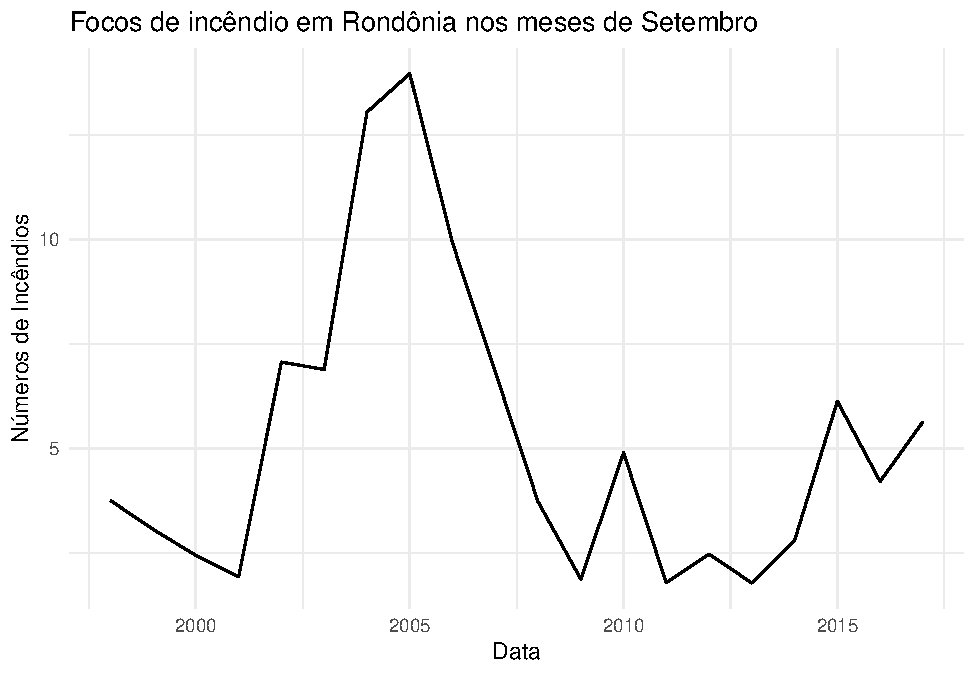
\includegraphics{00-intro_files/figure-latex/unnamed-chunk-63-1.pdf}

\hypertarget{rev}{%
\chapter{Revisão}\label{rev}}

Esse capítulo é uma breve revisão sobre conceitos estatísticos que são fundamentais para entender os conceitos da modelagem econométrica.

\hypertarget{aleatoriedade-a-essuxeancia-da-estatuxedstica}{%
\section{Aleatoriedade, a essência da estatística}\label{aleatoriedade-a-essuxeancia-da-estatuxedstica}}

Para iniciar qualquer curso em que são utilizadas técnicas estatísticas, é necessário esclarecer/fundamentar bem o conceito de aleatoriedade.

\begin{quote}
\emph{Na história antiga, os conceitos de chance e de aleatoriedade eram interligados ao conceito que era atribuído a destino. Várias pessoas da antiguidade jogavam dados para determinarem o destino, e posteriormente isso se desenvolveu em jogos de azar. A maioria das culturas usaram vários métodos de adivinhações para tentarem contornar a aleatoriedade e o destino, ou mesmo a dita sorte. A palavra aleatoriedade é utilizada para exprimir quebra de ordem, propósito, causa, ou imprevisibilidade em uma terminologia não científica. Um processo aleatório é o processo repetitivo cujo resultado não descreve um padrão determinístico, mas segue uma distribuição de probabilidade \href{https://pt.wikipedia.org/wiki/Aleatoriedade}{Wikipédia}.}
\end{quote}

\begin{figure}

{\centering 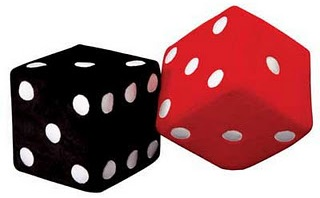
\includegraphics[width=0.33\linewidth]{Figuras/dados-vp} 

}

\caption{Dados}\label{fig:dados}
\end{figure}

As técnicas estatísticas surgem para encontrar algum \emph{padrão de variação}. Para tal tarefa é necessário formalizar e definir alguns conceitos, como são os casos de variável aleatória e distribuição de probabilidade.

\hypertarget{variuxe1vel-aleatuxf3ria}{%
\section{Variável aleatória}\label{variuxe1vel-aleatuxf3ria}}

Denomina-se \textbf{variável} uma propriedade (característica) qualquer das unidades da população para a qual foi definida uma unidade de medida, que pode ser quantitativa ou qualitativa. Observe que essa característica é comum a todos os indivíduos e portanto é uma característica da população. Em geral, queremos fazer afirmações sobre características e temos apenas informações de alguns indivíduos (amostra). Assim, toda afirmação feita a partir de uma amostra é passível de erros, ou seja, é uma aproximação. Além disso, em alguns casos não é possível ``medir'' toda a população e devemos pensar nessa característica como uma quantidade aleatória. Para isso, é necessário introduzirmos o conceito de \textbf{variável aleatória}.

\begin{definition}[Espaço Amostral]
\protect\hypertarget{def:EspacoAmostral}{}{\label{def:EspacoAmostral} \iffalse (Espaço Amostral) \fi{} }Espaço amostral de um \emph{experimento aleatório} (fenômeno que, mesmo repetidos várias vezes sob condições semelhantes, apresentam resultados imprevisíveis) é \textbf{qualquer} conjunto contendo todos os possíveis resultados do experimento. Aqui, sempre que não houver perigo de confusão, o espaço amostral de um experimento em questão será denotado por \(\Omega\).
\end{definition}

\begin{example}
\protect\hypertarget{exm:exampcel}{}{\label{exm:exampcel} }No seguinte experimento: derrubar o celular e observar a face voltada para cima, o espaço amostral é o conjunto \(\{\mathrm{Frontal}, \mathrm{Costas}\}\).
\end{example}

\begin{example}
\protect\hypertarget{exm:edados}{}{\label{exm:edados} }Se o experimento é lançar um dado de seis faces, o espaço amostral é \(\{1,2,3,4,5,6\}\).
\end{example}

\begin{example}
\protect\hypertarget{exm:exampespamost}{}{\label{exm:exampespamost} }Poderá perfeitamente existir mais de um espaço amostral adequado para um determinado experimento. No Exemplo \ref{exm:edados}, o conjunto \(\{1,2,3,4,5,6,7\}\) contém todos os possíveis resultados do experimento em questão (lançar um dado de seis faces). Assim, pela definição \ref{def:EspacoAmostral}, este conjunto é tão adequado como espaço amostral quanto o conjunto mais intuitivo \(\{1,2,3,4,5,6\}\). Até mesmo o conjunto dos números reais \(\mathbb{R}\) é adequado. Obviamente, sempre que possível é recomendável utilizar o conjunto mais \emph{natural} como espaço amostral, porém, do ponto de vista teórico, desde que o conjunto escolhido efetivamente contenha todos os possíveis resultados do experimento, não faz diferença alguma qual conjunto se está utilizando.
\end{example}

\begin{example}
\protect\hypertarget{exm:examexp}{}{\label{exm:examexp} }Nos exemplos anteriores, é possível (e muito fácil) determinar exatamente quais são todos os possíveis resultados dos experimentos em questão. Porém nem sempre este é o caso. Considere o experimento em que uma pessoa é escolhida ao acaso e sua altura (em metros) medida. Neste caso é difícil determinar precisamente o conjunto contendo exatamente todos os possíveis resultados do experimento. Com certeza o conjunto \([0,10]\) contém todas as possíveis alturas a serem registradas. O conjunto \([0,3]\) também. Por outro lado, será que o conjunto \([0,2.7]\) é apropriado? E \((0.3,2.7)\)?
\end{example}

Todo subconjunto de um espaço amostral é chamado \emph{evento}. Os
subconjuntos de um espaço amostral contendo apenas um elemento são
chamados de \emph{eventos elementares}.

Por exemplo, no lançamento de um dado de seis faces, \(\{5\}\) é um evento elementar. Outro evento possível é: \emph{a face superior é ímpar}, o que é equivalente ao subconjunto \(\{1,3,5\}\subset\Omega\). Outra possibilidade poderia ser verificar se a face obtida é superior a 3.

Existem ainda experimentos que podem ser vistos como ``compostos'' por natureza, como por exemplo o lançamento independente de um dado de seis faces e de uma moeda honesta, no qual anotamos a face superior do dado e a face da moeda. Neste caso, é fácil determinar um espaço amostral associado ao experimento que contenha exatamente todos os resultados possíveis. Este constituirá de pares contendo um número inteiro de 0 à 6, correspondente ao lançamento do dado e um elemento do conjunto \(\{\mathrm{Frontal},\mathrm{Costas}\}\), correspondente à queda do celular, ou seja, \(\Omega=\{(1, \mathrm{Frontal}), (1,\mathrm{costas}), \cdots, (6, \mathrm{Frontal}), (6,\mathrm{Costas})\}\). Uma outra maneira de representar isto é a partir do produto cartesiano dos espaços amostrais de cada um dos experimentos individuais, neste caso \(\Omega=\{1,2,3,4,5,6\}\times\{\mathrm{Frontal},\mathrm{Costas}\}\).

Espaços amostrais são importantes na definição de um \emph{espaço de probabilidade}. Um espaço de probabilidade \((\Omega, \mathcal{F},\mathcal{P})\) onde \(\Omega\) denota um espaço amostral qualquer, \(\mathcal{F}\) é um conjunto de eventos associado à \(\Omega\) satisfazendo certas propriedades (\(\sigma\)-algebra de eventos), e \(\mathcal{P}:\mathcal{F}\rightarrow[0,1]\) uma medida de probabilidade atribuindo valores em \([0,1]\) para cada evento de interesse em \(\mathcal{F}\) (a probabilidade dos eventos).

\begin{quote}
\emph{Uma \textbf{variável aleatória} é uma função do espaço amostral
\(\Omega\) nos reais, para a qual é possível calcular a
probabilidade de ocorrência de seus valores. Em geral, as
variáveis aleatórias são representadas por letras maiúsculas do
fim do alfabeto. Temos, para cada elemento \(\omega \in \Omega\), um
número real \(X(\omega)\) conforme a Figura \ref{fig:dados}.}
\end{quote}

\begin{figure}

{\centering 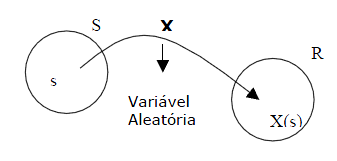
\includegraphics[width=0.33\linewidth]{Figuras/VA} 

}

\caption{Variável aleatória}\label{fig:va}
\end{figure}

Garantimos o cálculo de probabilidades com variáveis aleatórias ao exigir que, para qualquer \(I \subset \mathbb{R}\), o conjunto \(X^{-1}(I)\) seja um evento. Em outras palavras, o conjunto \(X^{-1}(I)\) é um
elemento de \(\mathcal{F}\), ou seja, \(X^{-1}(I) \in \mathcal{F}\). Lembremos que apenas os elementos de
\(\mathcal{F}\) têm atribuição de probabilidade. Em linguagem mais matemática, dizemos que uma variável aleatória é qualquer função mensurável em \((\Omega,\mathcal{F})\). Isto justifica dizer que a
variável \(X\) é \(\mathcal{F}\)-\emph{mensuravel}. Com frequência, faz-se menção ao espaço de probabilidade \((\Omega, \mathcal{F},\mathcal{P})\), para deixar claro o espaço amostral, a \(\sigma\)-álgebra e a probabilidade envolvidas. Formalmente, definimos

\begin{definition}
\protect\hypertarget{def:Def1}{}{\label{def:Def1} }Seja \((\Omega, \mathcal{F}, \mathcal{P})\) um espaço de
probabilidade. Denominamos de variável aleatória, qualquer função
\(X:\Omega \rightarrow \mathbb{R}\) tal que
\begin{equation*}
    X^{-1}(I)=\{\omega \in \Omega : X(\omega) \in I\} \in
    \mathcal{F},
\end{equation*}
para todo intervalo \(I \subset \mathbb{R}\). Em palavras, \(X\) é tal que sua
imagem inversa de intervalos \(I \subset \mathbb{R}\) pertencem a
\(\sigma\)-álgebra \(\mathcal{F}\).
\end{definition}

No que segue precisamos do conceito de cardinalidade de um conjunto. Em palavras simples, a cardinalidade de um conjunto é uma maneira de expressar a ``quantidade'' de elementos que este contém. Um conjunto ordenado \(A\) é dito \emph{finito} se contém um número finito de elementos. A cardinalidade de um conjunto finito nada mais é que o número de elementos que este contém. Por exemplo o conjunto \(A=\{1,2,9,15\}\) é finito e tem cardinalidade 4.

Por outro lado, a definição de cardinalidade para conjuntos infinitos é matematicamente muito mais complexa pois, no final das contas, a ideia é impor uma hierarquia, uma ``ordem'', no ``tamanho'' de conjuntos infinitos. Obviamente a cardinalidade de um conjunto infinito não pode ser expressa em números. Estamos interessados apenas em distinguir entre dois ``tamanhos'' de conjuntos infinitos: enumerável e não-enumerável. Por sorte, na maioria das vezes é possível utilizar apenas a intuição para resolver o problema. Intuitivamente, um conjunto ordenado \(A\) é dito ser infinito
enumerável (ou ainda, \emph{contável}) se dado um elemento qualquer de \(A\), podemos determinar quem é o próximo elemento do conjunto. Caso contrário, o conjunto é dito ser \emph{não-enumerável}. Por exemplo, o conjunto dos números naturais \(\mathbb{N}\) é infinito enumerável. De fato, dado qualquer número natural \(x\), o próximo é \(x+1\), obviamente. Já o conjunto \([0,1]\) é infinito não-enumerável. Por exemplo, dado o número \(0.5\in[0,1]\), qual é próximo elemento de \([0,1]\)? Poderíamos dizer 0.6, mas e 0.51? Este ainda está mais longe de 0.5 que \(0.501\). De fato \(0,5001\), \(0.50001\) etc. é uma sequência infinita de números em \([0,1]\) cada vez mais próxima de 0.5 de forma que não é possível determinar o próximo elemento na ordenação do conjunto.
Os conjuntos enumeráveis mais conhecidos são \(\mathbb{N}\), \(\mathbb{Z}\) e \(\mathbb{Q}\), sendo que este último é um pouco mais difícil de aplicar a regra intuitiva acima. Os conjuntos não enumeráveis mais conhecidos são \(\mathbb{R}\), \(\mathbb{R}\setminus\mathbb{Q}\), \(\mathbb{C}\).

\begin{definition}[Variável Aleatória Discreta]
\protect\hypertarget{def:vad}{}{\label{def:vad} \iffalse (Variável Aleatória Discreta) \fi{} }Se o conjunto dos possíveis valores da variável aleatória é finito ou infinito enumerável.
\end{definition}

\begin{definition}[Variável Aleatória Contínua]
\protect\hypertarget{def:vac}{}{\label{def:vac} \iffalse (Variável Aleatória Contínua) \fi{} }Se o conjunto dos possíveis valores da variável aleatória é infinito não-enumerável.
\end{definition}

Na prática, é comum a utilização de variáveis aleatórias contínuas pois estas são matematicamente mais simples de se tratar. Quando, por exemplo, falamos que a renda é uma v.a. contínua (na verdade ela é
discreta) é pela conveniência da aproximação.

\hypertarget{distribuiuxe7uxe3o-de-probabilidade}{%
\subsection{Distribuição de probabilidade}\label{distribuiuxe7uxe3o-de-probabilidade}}

A função que descreve as probabilidades da variável aleatória discreta \(X\) assumir os diferentes valores do espaço amostral é chamada de função massa de probabilidade. No caso de uma variável contínua, a probabilidade de uma variável aleatória assumir qualquer valor específico é 0. Neste caso o análogo da função massa de probabilidade é a função de densidade de probabilidade (abreviado f.d.p. ou ainda, do inglês, p.d.f.) que, em poucas palavras, descreve a variação instantânea da probabilidade no ponto. Para que uma função qualquer \(f\) seja uma densidade de probabilidade é necessário que

\begin{align}
 &f(x)\geq0\quad \mbox{ para todo } x\in\mathbb{R},\nonumber\\
&\int_{\mathbb{R}}f(x)dx=\int_{-\infty}^{\infty}f(x)dx=1.
\label{eq:fdensidade}
\end{align}

Como a probabilidade de ocorrência de um valor em particular de uma variávela aleatória contínua é sempre 0, probabilidades são discutidas em termos de intervalos, ou mesmo outros tipos de conjuntos. Essas probabilidades são obtidas por meio de
integração da função densidade no intervalo especificado. Por exemplo, seja \(X\) uma variávela aleatória com densidade \(f(x)\). Então \(P(a \leq X \leq b)\) é dada por
\[P(a \leq X \leq b)=\int_a^b f(x)dx.\]
Analogamente, para um conjunto \(A\subseteq \mathbb{R}\) qualquer,
\[P(X\in A)=\int_A f(x)dx.\]

A probabilidade de que a variável aleatória \(X\) assuma valores inferiores ou igual a um número \(x\in\mathbb{R}\), \(P(X\leq x)\), possui importancia intrínsica pois representa a probabilidade acumulada até o ponto \(x\). Por isso, para cada \(x\in\mathbb{R}\) fixo, denotamos esta probabilidade por
\[F(x)=P(X\leq x)\]
e a função assim definida \(F:\mathbb{R}\rightarrow[0,1]\) é chamada
de função de distribuição acumulada (denotada por f.d.a.), ou
somente função de distribuição. Note que se \(X\) é uma variável aleatória contínua com densidade \(f\),
\[F(x)=P(X \leq x)=\int_{-\infty}^x f(t)dt.\]

\hypertarget{distribuiuxe7uxf5es-conjunta-marginal-e-condicional}{%
\subsection{Distribuições conjunta, marginal e condicional}\label{distribuiuxe7uxf5es-conjunta-marginal-e-condicional}}

Geralmente estamos interessados não apenas numa variável aleatória mas na relação entre algumas variáveis aleatórias. Suponha que temos duas variáveis aleatórias, \(X\) e \(Y\). Agora além do comportamento probabilístico individual de \(X\) e \(Y\), caracterizado por suas funções de distribuições, digamos \(F_X\) e \(F_Y\), respectivamente, precisamos alguma forma de descrever o comportamento probabilístico conjunto de \(X\) e \(Y\). Para isso definimos a função de distribuição acumulada de \(X\) e \(Y\), denotada por \(F_{X,Y}\), por \[F_{X,Y}(x,y)=P(X\leq x, Y\leq y).\]

Se \(X\) e \(Y\) são ambas contínuas, podemos definir a densidade conjunta de \(X\) e \(Y\) denotada por \(f_{X,Y}\), como sendo a função que satisfaz
\[F_{X,Y}(x,y)=\int_{-\infty}^x \int_{-\infty}^y f_{X,Y}(z,w)dzdw.\]

A função de distribuição conjunta de um par de variáveis aleatórias \(X\) e \(Y\) caracteriza também os comportamentos probabilisticos de \(X\) e \(Y\) individualmente. De fato
\[F_X(x)=\lim_{y\rightarrow\infty}F_{X,Y}(x,y) \quad \mbox{ e }\quad F_Y(y)=\lim_{x\rightarrow\infty}F_{X,Y}(x,y)\]
e também
\begin{equation*}
f_X(x)=\int_{\mathbb{R}}f_{X,Y}(x,y)dy\quad\mbox{e}\quad f_Y(y)=\int_{\mathbb{R}}f_{X,Y}(x,y)dx.
\end{equation*}
Quando temos a função de distribuição conjunta de um par \(X\) e \(Y\) de variáveis aleatórias, dizemos que as densidades/distribuições individuais de \(X\) e \(Y\) são as densidades/distribuições marginais de \(X\) e \(Y\).

A função de distribuição condicional de \(X\) dado \(Y=y\) é descrita por
\[F_{X|Y}(x|y)=P(X\leq x|Y=y)
=\left\{\begin{array}{cc} \frac{P(X\leq x,Y=y)}{P(Y=y)}\,, & \mbox{ se $X$ é discreta e }P(Y=y)\neq 0 \,\,\, \\
\frac{\int_{-\infty}^x f_{X,Y}(t,y)dt}{f_y(y)}\,, & \mbox{ se $X$ é contínua e } f_Y(y)\neq 0\end{array}\right.
\]

\begin{itemize}
\tightlist
\item
  As densidades condicionais são:
\end{itemize}

~~~a) \(f_{X|Y}(x|y)\), que é a densidade de \(X\) dado \(Y=y\);

~~~b) \(f_{Y|X}(y|x)\), que é a densidade de \(Y\) dado \(X=x\).

Formalmente, temos a relação
\[F_{X|Y}(x|y)=\int_{-\infty}^xf_{X|Y}(t|y)dt\quad \mbox{e} \quad F_{Y|x}(y|x)=\int_{-\infty}^yf_{Y|X}(t|x)dt,\]
no caso em que \(X\) e \(Y\) são contínuas. Relações parecidas valem no caso em que \(X\) e \(Y\) são discretas, trocando-se integrais por somas e densidades por função massa de probabilidade.

A densidade conjunta pode ser escrita como o produto das
densidades marginal e condicional da seguinte forma:
\begin{eqnarray*}
f_{X,Y}(x,y)&=&f_X(x)f_{Y|X}(y|x)\\
      &=&f_Y(y)f_{X|Y}(x|y).
\end{eqnarray*}
Se \(f_{X,Y}(x,y)=f_X(x)f_Y(y)\) para todo \(x\) e \(y\), então \(X\) e \(Y\) são
chamadas de variáveis \emph{independentes}. Note que, se eles são
independentes,
\[f_{X|Y}(x|y)=f_X(x) \quad \mbox{e} \quad f_{Y|X}(y|x)=f_Y(y),\]
isto é, as distribuições condicionais são as mesmas que as marginais. Intuitivamente, quando \(X\) e \(Y\) são independentes \(X\) não carrega nenhuma informação útil a respeito de \(Y\), assim o fato de \(Y\) ser ou não conhecido é irrelevante para a determinação de \(X\).

\hypertarget{a-distribuiuxe7uxe3o-normal-e-distribuiuxe7uxf5es-relacionadas}{%
\section{A distribuição Normal e distribuições relacionadas}\label{a-distribuiuxe7uxe3o-normal-e-distribuiuxe7uxf5es-relacionadas}}

Existem algumas distribuições de probabilidade cujas probabilidades que, devido à sua utilização em diversas aplicações, valores de suas funções de distribuição são tabuladas. Dentre estas distribuições notáveis, podemos citar distribuição normal e as distribuições \(\chi^2\), \(t\) e \(F\), as quais discutiremos juntamente com as distribuições lognormal e normal bivariada. Existem diversas outras distribuições para as quais tabelas extensivas estão disponíveis. Como exemplos citamos as distribuições gama e beta. Na verdade, a distribuição \(\chi^2\) é um caso particular da distribuição gama, e as distribuições \(t\) e \(F\) são casos particulares da distribuição beta. Trataremos aqui apenas das citadas.

Existe um grande criticismo sobre a adequação da distribuição normal para descrever variáveis econômicas. Muitas vezes a distribuição normal de fato não é apropriada. Contudo, dois fatos tornam o estudo da distribuição normal importantes: primeiramente, embora existam problemas em que o uso da distribuição normal é questionável, existe um número muito maior de problemas em que o uso desta é totalmente apropriado. Segundo, mesmo que as variáveis não sejam normalmente distribuídas, pode-se considerar transformações de variáveis que façam com que as variáveis transformadas se tornem normalmente distribuídas.

\hypertarget{a-distribuiuxe7uxe3o-normal}{%
\subsection{A distribuição Normal}\label{a-distribuiuxe7uxe3o-normal}}

A distribuição normal, cuja densidade possui um formato que lembra um sino, é a distribuição
mais amplamente utilizada em aplicações estatísticas numa grande variedade de áreas. Dizemos que \(X\) tem distribuição normal com média \(\mu\in\mathbb{R}\) e variância \(\sigma^2>0\), denotado compactamente por \(X\sim N(\mu,\sigma^2)\), se sua função de densidade de probabilidade for dada por
\[f(x)=\frac{1}{\sigma \sqrt{2\pi}}\exp\left[-\frac{1}{2\sigma^2}(x-\mu)^2\right], \quad \mbox{para } x\in\mathbb{R}.\]
Os parâmetros \(\mu\) e \(\sigma^2\) são também
chamados de parâmetros de locação e escala, respectivamente.

\begin{figure}

{\centering 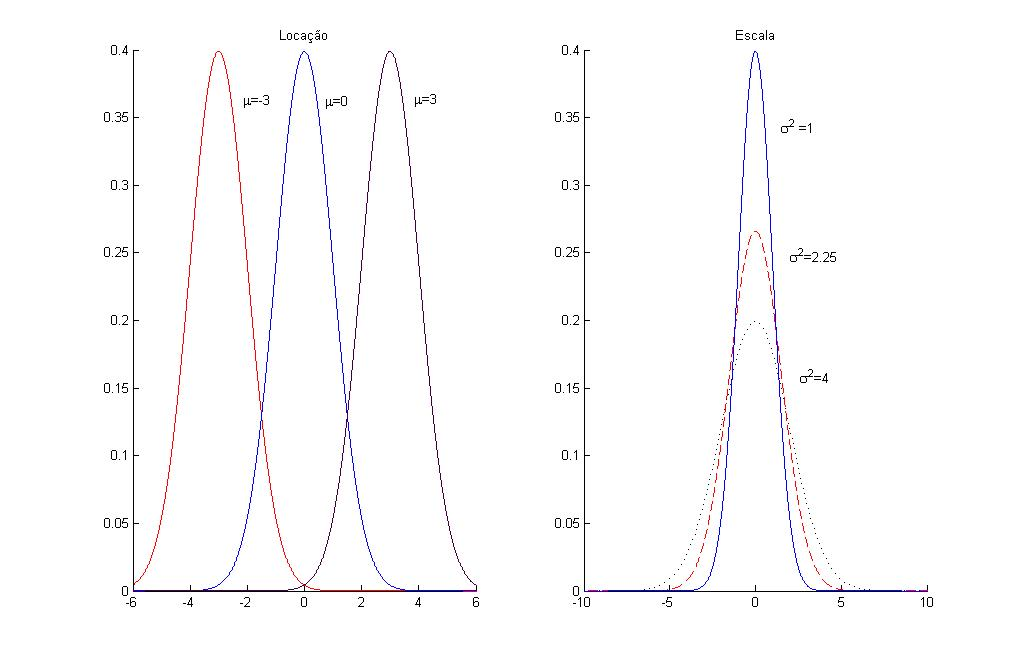
\includegraphics[width=0.8\linewidth]{Figuras/Loc_Esc_Normal} 

}

\caption{Função densidade Normal com diferentes parâmetros de locação  e escala.}\label{fig:LEN}
\end{figure}

Se \(\mu = 0\) e \(\sigma = 1\), a distribuição é chamada de ``distribuição normal padrão''
e a função de densidade de probabilidade reduz-se a,
\[f(x) = \frac{1}{\sqrt{2\pi}} \, e^{-\frac{x^2}{2}}.\]

Uma propriedade importante propriedade da distribuição normal é que qualquer
combinação linear de variáveis normalmente distribuídas também é
normalmente distribuída. De fato, pode-se mostrar que, se
\[X_1 \sim N(\mu_1,\sigma^2_1)
\quad \mbox{e} \quad X_2 \sim N(\mu_2,\sigma^2_2)\]
e a correlação entre \(X_1\) e \(X_2\) é \(\rho\), então
\[a_1X_1+a_2X_2 \sim N(a_1\mu_1+a_2\mu_2, a_1^2\sigma^2_1+a_2^2\sigma^2_2+2\rho
a_1a_2\sigma_1\sigma_2).\]
Em particular,

\[X_1+X_2 \sim N(\mu_1+\mu_2, \sigma^2_1+\sigma^2_2+2\rho \sigma_1\sigma_2)\]
e
\[X_1-X_2 \sim N(\mu_1-\mu_2, \sigma^2_1+\sigma^2_2-2\rho \sigma_1\sigma_2).\]

\hypertarget{distribuiuxe7uxf5es-relacionadas}{%
\subsection{Distribuições relacionadas}\label{distribuiuxe7uxf5es-relacionadas}}

Além da distribuição normal, há outras distribuições de probabilidade que usaremos com frequência. São elas as distribuições \(\chi^2\), \(t\) e \(F\), tabuladas no apêndice. Estas distribuições são derivadas da distribuição normal e definidas como descrito a seguir.

\hypertarget{distribuiuxe7uxe3o-chi2}{%
\subsubsection{\texorpdfstring{Distribuição \(\chi^2\)}{Distribuição \textbackslash chi\^{}2}}\label{distribuiuxe7uxe3o-chi2}}

A distribuição \(\chi^2\) é bastante importante em aplicações e é definida a partir da soma dos quadrados de variáveis normais. Mais especificamente, se \(X_1, X_2, \cdots, X_n\) são variáveis aleatórias independentes com distribuição normal padrão então
\[Q=\sum_{i=1}^n X_i^2\]
tem distribuição \(\chi^2\) com \(n\) graus de liberdade (g.l.), e escrevemos isso compactamente como \(Q \sim \chi_n^2\).

Se \(X_i \sim N(\mu, \sigma^2)\), então \(Q\) deve ser definido por

\[Q=\sum_{i=1}^n \frac{(X_i-\mu)^2}{\sigma^2}.\]
A distribuição \(\chi^2\) também satisfaz uma determinada ``propriedade de adição'',
no seguinte sentido: se \(Z_1 \sim \chi_n^2\) e \(Z_2 \sim \chi_m^2\) e \(Z_1\) e \(Z_2\) são
independentes, então \(Z_1+Z_2 \sim \chi^2_{n+m}\). Note que esta propriedade de adição é bem mais restritiva que aquela da distribuição normal, já que exige independência para que a simples soma das variáveis satisfaçam à propriedade (para normal, a propriedade vale para combinações lineares quaisquer), mas ainda assim é muito útil na prática.

\hypertarget{distribuiuxe7uxe3o-t}{%
\subsubsection{\texorpdfstring{Distribuição \(t\)}{Distribuição t}}\label{distribuiuxe7uxe3o-t}}

Se \(X \sim N(0,1)\), \(Y \sim \chi^2_n\), e \(X\) e \(Y\) são independentes, a variável
\[T=\frac{X}{\sqrt{Y/n}}=\frac{\sqrt{n}X}{\sqrt{Y}}\]
possui distribuição \(t\) com \(n\) g.l. Escrevemos isso como \(T \sim t_n\). O subscrito \(n\) novamente
denota os g.l. Assim como a distribuição normal, a distribuição \(t\) é uma distribuição de probabilidade simétrica, com forma lembrando um sino, sendo porém mais achatada e com caudas mais ``pesadas'' que a normal. Quando o número de graus de liberdade \(n\) de uma variável \(t_n\) tende ao infinito, obtemos a distribuição normal. Em outras palavras, quando os graus de liberdade de uma variável aleatória com distribuição \(t_n\) for grande, esta tem comportamento probabilístico muito similar ao de uma normal.

\hypertarget{distribuiuxe7uxe3o-f}{%
\subsubsection{\texorpdfstring{Distribuição \(F\)}{Distribuição F}}\label{distribuiuxe7uxe3o-f}}

Se \(Y_1 \sim \chi^2_{n1}\), \(Y_2 \sim \chi^2_{n2}\) e \(Y_1\) e \(Y_2\) são independentes, a variável
\[F=\frac{Y_1/n_1}{Y_2/n_2}=\frac{n_2Y_1}{n_1Y_2}\]
é dita possuir distribuição \(F\) com \(n_1\) e \(n_2\) g.l. Escrevemos isso como \(F\sim F_{n_1,n_2}\). O primeiro subscrito \(n_1\), refere-se aos g.l. do numerador, e o segundo subscrito, \(n_2\), refere-se aos g.l. do denominador.

\begin{figure}

{\centering 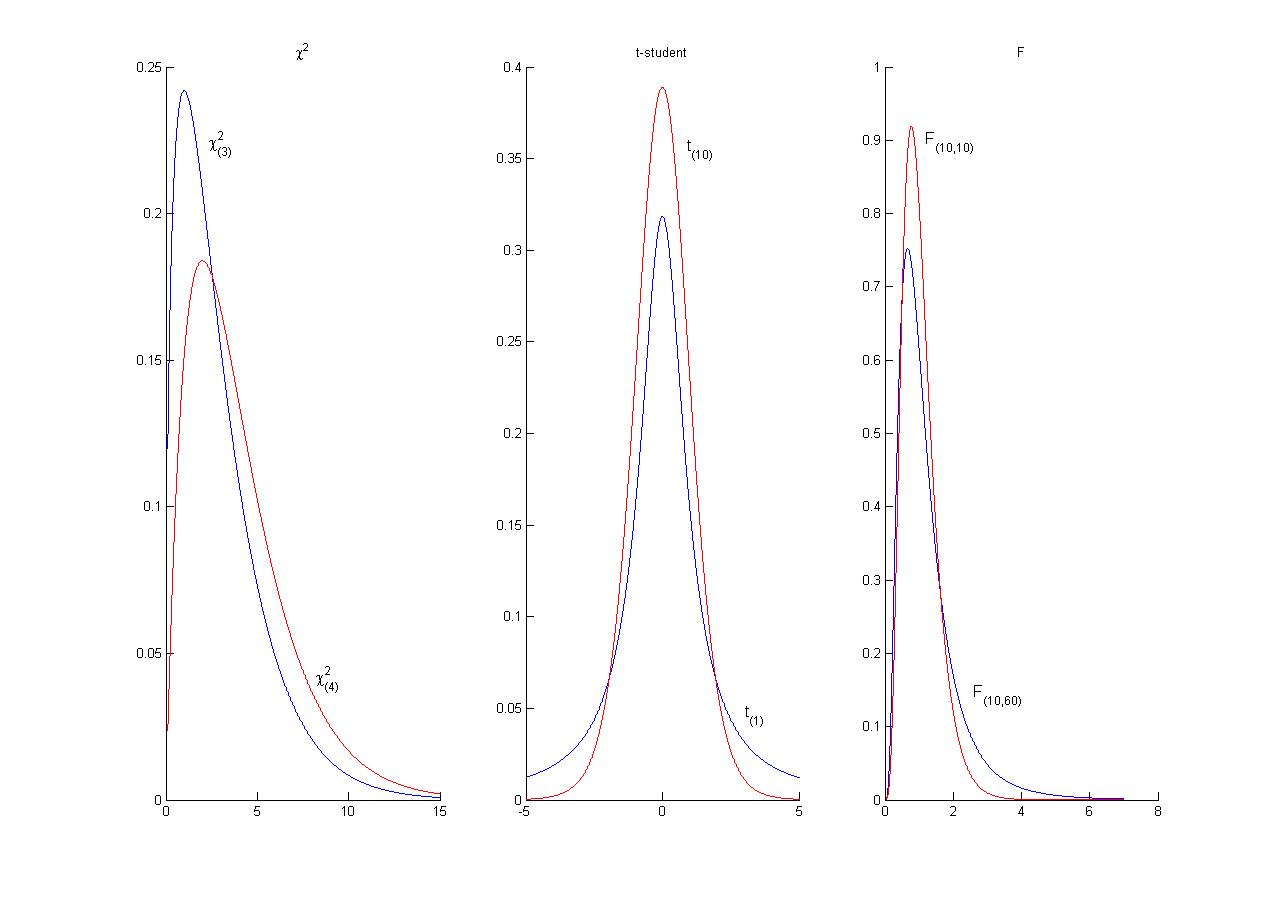
\includegraphics[width=0.8\linewidth]{Figuras/chi_t_F_density} 

}

\caption{Função densidade Qui-Quadrado, t-Student e F-Snedecor. Em parênteses os graus de liberdade.}\label{fig:len}
\end{figure}

\hypertarget{paruxe2metros-estimadores-e-valores-estimados}{%
\section{Parâmetros, estimadores e valores estimados}\label{paruxe2metros-estimadores-e-valores-estimados}}

Considere o deslocamento de uma partícula no vácuo, em superfície sem atrito. Aprendemos cedo que a velocidade da partícula num instante de tempo \(t\), \(v_t\), é dada por \(v_t=v_0+at\), onde \(v_0\) é a velocidade inicial da partícula, \(a>0\) é a aceleração aplicada na partícula, neste caso assumida constante. Neste modelo idealizado, a velocidade de uma partícula é uma função linear do tempo, cujo gráfico é apresentado na Figura \ref{fig:gfig1}(a).

Um grupo de pesquisadores realizou o seguinte experimento: numa superfície lisa, porém não absolutamente sem atrito, ao ar livre (isto é, na presença de vento, partículas de poeira, etc.) uma partícula foi acelerada à uma determinada aceleração desconhecida, mas constante em cada repetição do experimento, à partir de uma velocidade inicial desconhecida, mas também constante em cada repetição do experimento. Após um determinado tempo \(t\) a velocidade da partícula foi medida. Como resultados obtemos pares \((v_i,t_i)\) representando a \(i\)-ésima observação da velocidade da partícula, medida no tempo \(t_i\). Os resultados estão apresentados na Figura \ref{fig:gfig1}(b). Nosso interesse é determinar a velocidade inicial da partícula e a aceleração, que são chamados de parâmetros populacionais. Note que devido às condições não serem ideais, os dados não estão perfeitamente alinhados em uma reta como o estipulado na teoria, mas estão aproximadamente alinhados. Os desvios da reta ``esperada'' podem ser interpretados como sendo aleatórios, e são devidos aos vários fatores que estão fora de nosso controle, como atrito, vento, partículas em suspensão no ar, etc, fatores que estão em desalinho com a teoria.

Para estimar os parâmetros \(a\) e \(v_0\), que denotaremos por \(\hat{a}\) e \(\hat{v_0}\), podemos utilizar os estimadores de Mínimos Quadráticos Ordinários que conhecemos, neste caso, dados por (mais detalhes serão fornecidos adiante)
\[\hat a=\frac{\sum_{i=1}^n(v_i-\bar v)(t_i-\bar t)}{\sum_{i=1}^n(t_i-\bar t)^2} \quad\mbox{ e }\quad \hat{v_0}=\bar{v}-\hat{a}\bar{t},\]
onde \(\bar{v}\) denota a média das velocidades e \(\bar{t}\) denota a média dos tempos observados. Note que, fornecidos os dados para o estimador, ele retorna dois valores sendo eles a estimativa dos parâmetros \(a\) e \(v_0\) baseados nos dados. Note que mudando os dados, o estimador continua sendo o mesmo, mas os valores retornados por ele, as estimativas, mudarão. À partir dessas estimativas obtemos a reta apresentada na Figura \ref{fig:gfig1}(c)

Na resolução do problema aparecem 3 objetos eminentemente diferentes, cada um deles fundamental na solução do problema e que devem ser entendidos com clareza. Primeiramente temos os parâmetros populacionais, que são os valores de interesse, mas que nos são desconhecidos. Baseado numa amostra, gostaríamos, de alguma forma identificar, esses parâmetros. Segundo temos um estimador, que é uma função dos dados. Quando alimentado de dados estes estimadores retornam valores. Os valores retornados pelo estimador compreendem o terceiro objeto mencionado: são os valores estimados dos parâmetros populacionais.

Esta distinção entre parâmetro, estimador e valor estimado é essencial e está no coração das aplicações de estatística à dados reais.

\begin{figure}
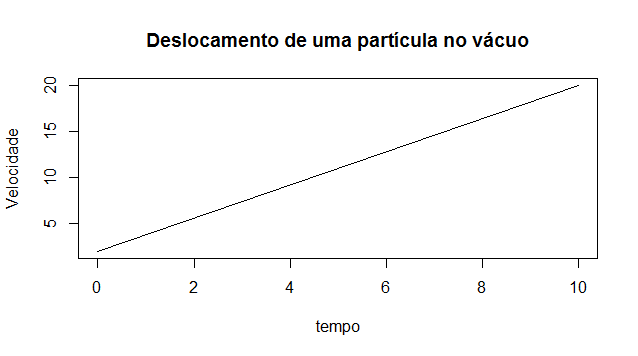
\includegraphics[width=0.3\linewidth]{Figuras/gfig1a} 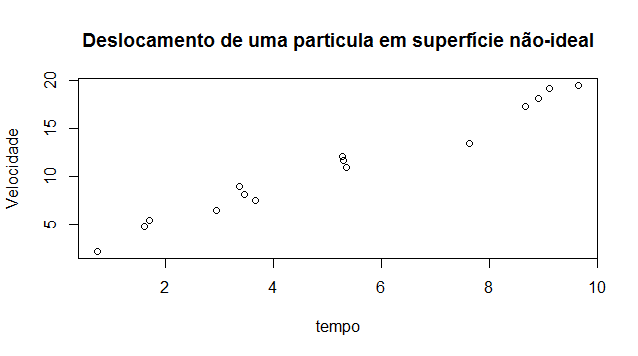
\includegraphics[width=0.3\linewidth]{Figuras/gfig1b} 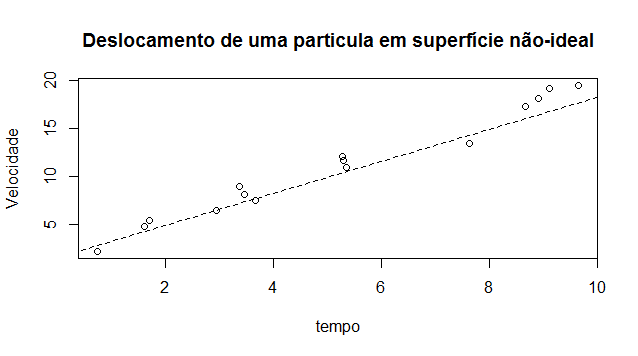
\includegraphics[width=0.3\linewidth]{Figuras/gfig1c} \caption{Partícula}\label{fig:gfig1}
\end{figure}

\hypertarget{propriedades-de-variuxe1veis-aleatuxf3rias}{%
\section{Propriedades de variáveis aleatórias}\label{propriedades-de-variuxe1veis-aleatuxf3rias}}

\hypertarget{muxe9dia-valor-esperado-ou-esperanuxe7a-matemuxe1tica}{%
\subsection{Média, valor esperado ou esperança matemática}\label{muxe9dia-valor-esperado-ou-esperanuxe7a-matemuxe1tica}}

A Média ou valor esperado, ou ainda a esperança matemática de uma variável aleatória representa o valor médio assumido pela variável em questão. Esta pode ser interpretada como a média ponderada de cada valor assumido pela variável ponderado pela sua probabilidade de ocorrência.

\begin{definition}[Média, valor esperado ou esperança matemática de variáveis aleatórias discretas.]
\protect\hypertarget{def:defmean}{}{\label{def:defmean} \iffalse (Média, valor esperado ou esperança matemática de variáveis aleatórias discretas.) \fi{} }Suponha que \(X\) seja uma variável aleatória discreta assumindo \(n\) valores diferentes \(x_1,\cdots x_n\) com probabilidades \(p_1,\cdots,p_n\), respectivamente. Então a média, ou valor esperado ou anda a esperança da variável \(X\) é definida por
\[\mathbb{E}(X)=x_1p_1+x_2p_2+\cdots+x_np_n=\sum_{i=1}^nx_ip_i.\]
\end{definition}

Observe que, no caso discreto, a esperança de uma variável \(X\) nada mais é do que a média ponderada de cada valor assumido pela variável pela sua probabilidade de ocorrência.

\begin{example}
\protect\hypertarget{exm:exemploEspdado}{}{\label{exm:exemploEspdado} }Seja \(X\) o valor da face superior obtida no lançamento de um
dado equilibrado. Neste caso temos
\(P(X=1)=P(X=2)=P(X=3)=P(X=4)=P(X=5)=P(X=6)=\frac{1}{6}\), ou seja
\(p_1=p_2=p_3=p_4=p_5=p_6=\frac{1}{6}\). Segue que
\begin{eqnarray*}
\mathbb{E}(X)&=&\sum_{i=1}^6p_ix_i= \frac{1}{6}.1+\frac{1}{6}.2+\frac{1}{6}.3+\frac{1}{6}.4+\frac{1}{6}.5+\frac{1}{6}.6\\
     &=&\frac{1}{6}(1+2+3+4+5+6)=\frac{1}{6}.\frac{6(6+1)}{2}\\
     &=&\frac{21}{6}=\frac{7}{2}=3,5.
\end{eqnarray*}
O valor 3,5 obtido no resultado deve ser interpretado da seguinte forma: se jogarmos um dado equilibrado um número grande de vezes e calcularmos a média dos valores obtidos, ele será próximo à 3,5. De fato, se fosse possível repertir o experimento um número infinito de vezes, a média dos resultados convergiria para 3,5.
\end{example}

\begin{definition}[Valor Esperado de $g(X)$.]
\protect\hypertarget{def:defexper}{}{\label{def:defexper} \iffalse (Valor Esperado de \(g(X)\).) \fi{} }Seja \(X\) uma variável aleatória discreta assumindo \(n\) valores diferentes \(x_1,\cdots x_n\) com probabilidades \(p_1,\cdots,p_n\), respectivamente. Seja \(g\) uma função definida na imagem da variável aleatória de \(X\). Então \(\mathbb{E}(g(X))\) é dado por
\[\mathbb{E}(g(X))=g(x_1)p_1+ \cdots + g(x_n)p_n=\sum_{i=1}^n g(x_i)p_i.\]
\end{definition}

\begin{example}
\protect\hypertarget{exm:exemploEspdado2}{}{\label{exm:exemploEspdado2} }Para o Exemplo \label{exemplo_Esp_dado} considere
\(g(X)=X^2.\) Obtemos
\begin{eqnarray*}
\mathbb{E}(X^2)&=&\sum_{i=1}^6p_ix_i^2= \frac{1}{6}.1+\frac{1}{6}.4+\frac{1}{6}.9+\frac{1}{6}.16+\frac{1}{6}.25+\frac{1}{6}.36\\
     &=&\frac{1}{6}(1+4+9+16+25+36)=\frac{1}{6}.\frac{6(6+1)(12+1)}{6}\\
     &=&\frac{91}{6}=15,16666.
\end{eqnarray*}
Note que \(\mathbb{E}(X^2)\neq \mathbb{E}(X)^2\).
\end{example}

\begin{definition}[Esperança de variáveis aleatórias contínuas,]
\protect\hypertarget{def:defexc}{}{\label{def:defexc} \iffalse (Esperança de variáveis aleatórias contínuas,) \fi{} }Supondo que \(X\) seja uma variável aleatória contínua com função de densidade de probabilidade \(f\), definimos a esperança de \(X\) por
\[\mathbb{E}(X)=\int_{-\infty}^{\infty}xf(x)dx.\]
O valor esperado de uma função integrável qualquer de \(X\), digamos \(g(X)\) é definido por
\[\mathbb{E}(g(X))=\int_{-\infty}^{\infty}g(x)f(x)dx.\]
\end{definition}

\begin{example}
\protect\hypertarget{exm:exmmeanNormal}{}{\label{exm:exmmeanNormal} } Se \(X\sim N(\mu,\sigma^2)\), então \(\mathbb{E}(X)=\mu\), como pode ser facilmente computado.
\end{example}

\hypertarget{propriedades-da-esperanuxe7a}{%
\subsection{Propriedades da Esperança}\label{propriedades-da-esperanuxe7a}}

No que segue, assumimos que \(X, Y\) são variáveis aleatórias e \(a, b, c\) são constantes reais.

\begin{itemize}
\item
  \textbf{E1} - \(\mathbb{E}(a) = a;\)
\item
  \textbf{E2} - \(\mathbb{E}(a + X) = a + \mathbb{E}(X);\)
\item
  \textbf{E3} - \(\mathbb{E}(b X) = b \mathbb{E}(X);\)
\item
  \textbf{E4} - \(\mathbb{E}(a + b X) = a + b \mathbb{E}(X);\)
\item
  \textbf{E5} - \(\mathbb{E}(X + Y) = \mathbb{E}(X) + \mathbb{E}(Y);\)
\item
  \textbf{E6} - \(\mathbb{E}(a + bX + cY) = a + b \mathbb{E}(X) + c \mathbb{E}(Y);\)
\end{itemize}

Estas propriedades podem ser generalizadas para qualquer número de variáveis aleatórias.

Em particular, segue a esperança de uma combinação linear de variáveis aleatórias
é a combinação linear das suas esperança, isto é, se \(X_1,\cdots,X_n\) são variáveis aleatórias e \(a_1,\cdots,a_n\) são constantes reais,

\begin{itemize}
\tightlist
\item
  \textbf{E7} - \(\displaystyle{\mathbb{E}\bigg(\sum_{i=1}^na_iX_i\bigg)= \sum_{i=1}^na_i\mathbb{E}(X_i)}.\)
\end{itemize}

Por esse motivo, a função \(\mathbb{E}(\cdot)\) que associa a cada variável aleatória o seu valor esperado é um \emph{operador linear}, chamado de \emph{operador esperança}.

Em geral, temos que \(\mathbb{E}(X Y) \neq \mathbb{E}(X) \mathbb{E}(Y)\). Porém, no caso particular em que \(X\) e \(Y\) são variáveis aleatórias independentes, a igualdade é válida, isto é,
\[\mathbb{E}(X Y) = \mathbb{E}(X) \mathbb{E}(Y)\quad \mbox{se, e somente se, $X$ e $Y$ são independentes}.\]

\hypertarget{variuxe2ncia}{%
\subsection{Variância}\label{variuxe2ncia}}

Seja \(X\) uma variável aleatória (contínua ou discreta)e defina \(\mu = \mathbb{E}(X)\). Então a variância de \(X\) é definida por

\begin{equation}
\mbox{Var}(X)={\mathbb{E}}[(X-\mu)^2)]=\mathbb{E}(X^2)-[\mathbb{E}(X)]^2.
\label{eq:var}
\end{equation}

Podemos interpretar a variância como sendo o valor esperado do quadrado do desvio de \(X\) da sua própria média. Em linguagem comum isto pode ser expresso como \emph{A média do quadrado da distância de cada ponto até a média}. É assim a \emph{média do quadrado dos desvios}. A variância da variável aleatória \(X\) é geralmente designada por \(\mbox{Var}(X)\), \(\sigma^2_X\), ou simplesmente \(\sigma^2\). A variância é uma medida de dispersão dos dados e sua unidade é a unidade dos dados elevada ao quadrado. Lembramos que a raiz quadrada positiva da variância determina o chamado desvio padrão de \(X\).

\hypertarget{covariuxe2ncia}{%
\subsection{Covariância}\label{covariuxe2ncia}}

A covariância entre duas variáveis aleatórias \(X\) e \(Y\) com \({\mathbb{E}}(X)=\mu_{X}\) e
\({\mathbb{E}}(Y)=\mu_{Y}\) é definida por
\[\mbox{Cov}(X, Y) = {\mathbb{E}}[(X - \mu_{X}) (Y - \mu_{Y})].\]

Desenvolvendo a expressão para a covariância, temos:
\begin{align*}
\mbox{Cov}(X, Y) &= {\mathbb{E}}\big[(X - \mu_{X}) (Y - \mu_{Y})\big]\\
&={\mathbb{E}}\big[(X - \mathbb{E}(X)) (Y - {\mathbb{E}}(Y))\big]\\
&={\mathbb{E}}\big[XY - X{\mathbb{E}}(Y) - Y{\mathbb{E}}(X) + {\mathbb{E}}(X){\mathbb{E}}(Y)\big].
\end{align*}
Usando a propriedade de que a esperança da soma entre duas variáveis aleatórias é igual a soma das esperanças, segue que

\begin{align}
\mbox{Cov}(X, Y) &= {\mathbb{E}}(XY) - {\mathbb{E}}\big[X{\mathbb{E}}(Y)\big] - {\mathbb{E}}\big[Y{\mathbb{E}}(X)\big] +  {\mathbb{E}}\big[{\mathbb{E}}(X){\mathbb{E}}(Y)\big]\nonumber\\
&= {\mathbb{E}}(XY) - {\mathbb{E}}(Y){\mathbb{E}}(X) - {\mathbb{E}}(X){\mathbb{E}}(Y) + {\mathbb{E}}(X){\mathbb{E}}(Y)\nonumber\\
&=\mathbb{E}(X Y) - \mathbb{E}(X) \mathbb{E}(Y)
\label{eq:aquela}
\end{align}
Note que quando \(X\) e \(Y\) são independentes, temos que \(\mathbb{E}(XY)=\mathbb{E}(X)\mathbb{E}(Y)\) de onde segue que \(\mbox{Cov}(X,Y)=0\). A recíproca, porém, não é verdadeira pois existem exemplos de variáveis dependentes que possuem covariância nula. Observe ainda que da expressão \eqref{eq:aquela} podemos concluir que a covariância é uma forma de medir o quão ``distante'' \(X\) e \(Y\) estão de ser independentes.

\hypertarget{correlauxe7uxe3o}{%
\subsection{Correlação}\label{correlauxe7uxe3o}}

A correlação, também chamada de coeficiente de correlação, indica a força e a direção do relacionamento linear entre duas variáveis aleatórias, se existir. A correlação entre duas variáveis \(X\) e \(Y\) com \(0<\mbox{Var}(X)<\infty\) e \(0<\mbox{Var}(Y)<\infty\), denotado por \(\mbox{Cor}(X,Y)\) ou \(\rho_{_{X,Y}}\), é definida como
\[\mbox{Cor}(X,Y)=\rho_{_{X,Y}}=\frac{\mbox{Cov}(X,Y)}{  \sqrt{\mbox{Var}(X)\mbox{Var}(Y)}}=\frac{\mathbb{E}(XY)-\mathbb{E}(X)\mathbb{E}(Y)}{\sqrt{\mathbb{E}(X^2)-\mathbb{E}^2(X)}~\sqrt{\mathbb{E}(Y^2)-\mathbb{E}^2(Y)}}.\]
Note que a correlação entre \(X\) e \(Y\) nada mais é do que a covariância entre \(X\) e \(Y\) normalizada por seus desvios padrões. Esta normalização acaba dando à correlação uma interpretabilidade ausente na covariância como veremos a seguir.

Observe ainda que, quando \(\mbox{Cov}(X,Y)=0\), temos \(\mbox{Cor}(X,Y)=0\) também e \(X\) e \(Y\) são ditos ser variáveis não-correlacionadas.

\hypertarget{propriedades-da-variuxe2ncia-covariuxe2ncia-e-correlauxe7uxe3o}{%
\subsection{Propriedades da variância, covariância e correlação}\label{propriedades-da-variuxe2ncia-covariuxe2ncia-e-correlauxe7uxe3o}}

Se \(a\) e \(b\) forem constantes reais e \(X\) uma variável aleatória cuja variância está definida, então:

\begin{itemize}
\item
  \textbf{V1} - \(\mbox{Var}(aX+b)=a^2\mbox{Var}(X);\)
\item
  \textbf{V2} - \(\mbox{Var}(X+Y) =\mbox{Var}(X) + \mbox{Var}(Y)+ 2 \mbox{Cov}(X, Y).\)
\end{itemize}

Da propriedade V1 segue que a variância de uma constante é zero. Além disso, se a variância de uma variável aleatória é zero, então esta variável assume um único valor com probabilidade 1. Da propriedade V2 segue que se \(X\) e \(Y\) são não-correlacionados, então a variância da soma é a soma das variâncias.

Suponha agora que \(X\) e \(Y\) são variáveis aleatórias e \(a\), \(b\), \(c\) e \(d\) são constantes reais. Então

\begin{itemize}
\item
  \textbf{Cv1} - \(\mbox{Cov}(X, X) = \mbox{Var}(X)\);
\item
  \textbf{Cv2} - \(\mbox{Cov}(X, Y) = \mbox{Cov}(Y,X)\);
\item
  \textbf{Cv3} - \(\mbox{Cov}(aX + b, cY + d) = ac\mbox{Cov}(X, Y)\);
\item
  \textbf{Cv4} - \(\displaystyle{\mbox{Cov}\bigg(\sum_{i=1}^n{X_i}, \sum_{j=1}^m{Y_j}\bigg)= \sum_{i=1}^n\sum_{j=1}^m\mbox{Cov}(X_i, Y_j)}\).
\end{itemize}

Como mencionado anteriormente, se \(X\) e \(Y\) são independentes, então \(\mbox{Cov}(X,Y)=0\).

A correlação, por sua vez, possui as seguintes propriedades:

\begin{itemize}
\item
  \textbf{Cr1} - \(\left| \mbox{Cor}(X,Y)\right|\leq 1\);
\item
  \textbf{Cr2} - \(\mbox{Cor}(X,Y) = 1\) se, e somente se, \(X\) é diretamente proporcional a \(Y\) no sentido de que \(X=a+bY\) para \(a\in\mathbb{R}\) e \(b>0\);
\item
  \textbf{Cr3} - \(\mbox{Cor}(X, Y) = -1\) se, e somente se, \(X\) é inversamente proporcional a \(Y\) no sentido de que \(X=a+bY\) para \(a\in\mathbb{R}\) e \(b<0\);
\item
  \textbf{Cr4} - \(\mbox{Cor}(X, Y) = \mbox{Cor}(Y,X)\);
\item
  \textbf{Cr5} - \(\mbox{Cor}(aX + b, cY + d) = \mathrm{sign}(ac)\mbox{Cor}(X, Y)\), onde a função sign\((x)\) é a função sinal de \(x\), sendo igual a \(-1\), se \(x<0\), 1 se \(x>0\) e \(0\) se \(x=0\);
\item
  \textbf{Cr6} - Se \(X\) e \(Y\) são independentes, então \(\mbox{Cor}(X,Y)=0\). A reciproca, porém, não é verdadeira.
\end{itemize}

\hypertarget{estimadores}{%
\section{Estimadores}\label{estimadores}}

Dada uma amostra \(x_1,x_2,\cdots,x_n\) de uma variável aleatória \(X\), o estimador de \(\mathbb{E}(X)\) é simplesmente a média aritmética dos dados:

\[ \overline{X}=\frac{1}{n}\sum_{i=1}^{n}x_i.\]

Com relação à variância de \(X\), existem dois estimadores muito utilizados na prática. O estimador da variância de \(X\) obtido pelo método de máxima verossimilhança é dado por

\[\hat{\sigma}_X^2=\frac{1}{n}\sum_{i=1}^{n}(x_i-\overline{x})^2=\frac1n\bigg(\sum_{i=1}^nx_i^2-n\overline{x}^2\bigg).\]

Pode-se mostrar que, embora consistente, este estimador é viesado em amostras finitas. Um estimador consistente e não-viesado em amostras finitas é dado por
\[ {S}_X^2=\frac{1}{n-1}\sum_{i=1}^{n}(x_i-\overline{x})^2=\frac1{n-1}\bigg(\sum_{i=1}^nx_i^2-n\overline{x}^2\bigg).\]

Observe que para \(n\) grandes, a diferença entre os estimadores \(\hat\sigma^2\) e \(S^2\) é irrelevante. Em amostras pequenas, porém, o estimador \(S^2\) apresenta uma performance melhor.

Seja \(x_1,x_2,\cdots,x_n\) e \(y_1,y_2,\cdots,y_n\) amostras aleatórias das variáveis
aleatórias \(X\) e \(Y\). Então um estimador para a covariância entre \(X\) e \(Y\) é dado por
\[\hat{ \gamma}_{_{X,Y}}=\frac{1}{n-1}\sum_{i=1}^{n}(x_i-\overline{x})(y_i-\overline{y})=\frac1{n-1}\bigg(\sum_{i=1}^{n}x_iy_i-n\overline{x}\overline{y}\bigg).\]

Um estimador para a correlação entre \(X\) e \(Y\) é dado por

\[\hat{\rho}_{_{X,Y}} = \frac{\hat{ \gamma}_{_{X,Y}}}{S_XS_Y}.\]

\hypertarget{propriedades-dos-estimadores}{%
\subsection{Propriedades dos estimadores}\label{propriedades-dos-estimadores}}

Dado que temos alguns estimadores definidos acima, é interessante estudar algumas
das propriedades qualitativas dos estimadores que nos permitam determinar qual estimador é \emph{``bom''} e qual não é. É também importante definir critérios para compar diversos estimadores.

\hypertarget{vuxedcioviuxe9s}{%
\subsection{Vício/Viés}\label{vuxedcioviuxe9s}}

Seja \(\hat{\theta}\) um estimador do parâmetro \(\theta\). o vício/viés (bias, em inglês) é definido como

\begin{equation}
 b(\hat{\theta})=\mathbb{E}(\hat{\theta})-\theta.
 \label{eq:vies}
\end{equation}

Se \(b(\hat\theta)=0\) segue que \(\mathbb{E}(\hat{\theta})-\theta\) e, neste caso, dizemos que \(\hat\theta\) é não-viciado ou não-viesado para o parâmetro \(\theta\).

\hypertarget{consistuxeancia}{%
\subsection{Consistência}\label{consistuxeancia}}

Em estatística, uma seqüência de estimadores para o parâmetro \(\theta\) é dito ser consistente (ou assintoticamente consistente) se esta sequência converge em probabilidade para \(\theta\). Isso significa que as distribuições dos estimadores tornar-se mais e mais concentrados perto do verdadeiro valor do parâmetro a ser estimado, de modo que a probabilidade do estimador ser arbitrariamente perto \(\theta\) converge para um.

\hypertarget{eficiuxeancia}{%
\subsection{Eficiência}\label{eficiuxeancia}}

Um estimador de \(\theta\) é dito ser eficiente se for não viesado e sua variância for menor ou igual a variância de qualquer outro estimador \(\hat{\theta}\), ou seja,
\[
\mbox{Var}(\hat{\theta}_0)\leq \mbox{Var}(\hat{\theta}),\,\,\,\,
        \mbox{para  qualquer outro estimador}\,\,\,\,\, \hat{\theta}\,\,\, \mbox{ de }\theta.
\]

Na figura abaixo podemos observar a diferença entre vício e eficiência. Estes conceitos estão relacionados à média e à variância, respectivamente.

\begin{figure}

{\centering 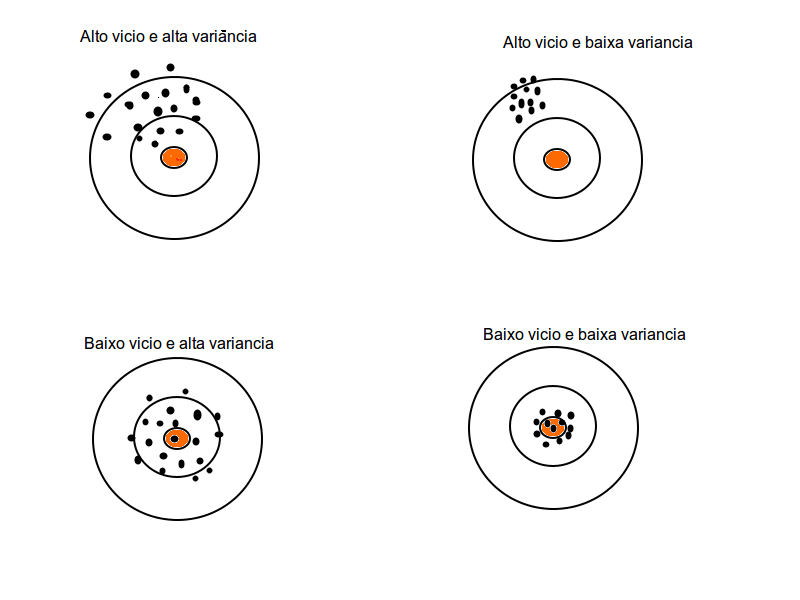
\includegraphics[width=0.8\linewidth]{Figuras/vicio_var} 

}

\caption{Diferença entre vício e eficiência.}\label{fig:Propest}
\end{figure}

\hypertarget{erro-quadruxe1tico-muxe9dio-eqm}{%
\subsection{Erro quadrático médio (EQM)}\label{erro-quadruxe1tico-muxe9dio-eqm}}

O erro quadrático médio de um estimador \(\hat{\theta}\) de \(\theta\) é definido como
\begin{equation}
EQM(\hat\theta) = \mathbb{E}(\hat{\theta} - \theta)^2.
\label{eq:eqm}
\end{equation}

Podemos reescrever esta ultima expressão como
\[EQM (\hat\theta) = \mbox{Var}(\theta) + [\mathbb{E}(\theta) - \theta]^2 =\mbox{Var}(\hat{\theta})+b(\hat{\theta}).\]

Assim, o erro quadrático médio é definido como a variância do estimador mais o quadrado do seu viés. Podemos entender o EQM como sendo uma medida da performance de um estimador em relação ao seu vício e variância. Note que EQM\((\theta)=\mbox{Var}(\theta)\) sempre que o estimador for não-viciado.

\hypertarget{vuxedcio-versus-vvariuxe2ncia-muxednima}{%
\subsection{Vício versus Vvariância mínima}\label{vuxedcio-versus-vvariuxe2ncia-muxednima}}

O erro quadrático médio utilizado na comparação entre um ou mais estimadores para um
mesmo parâmetro \(\theta\). Podemos observar de \eqref{eq:eqm} que, no cálculo do EQM, existe um balanço entre vício e variância. Naturalmente, estimadores eficientes apresentarão um EQM mínimo dentre os estimadores não-viciados de \(\theta\). Muitas vezes, porém, pode ser mais vantajoso do ponto de vista prático a utilização de um estimador viciado mas com variância pequena em detrimento a um estimador de maior variância, mas que seja não-viciado. Isto ocorre por que se a variância de um estimado é muito grande, é grande a chance de uma estimativa esteja longe do verdadeiro valor do parâmetro, mesmo que o estimador seja não-viciado. Este é um ponto importante a ser observado quando da escolha de um estimador para um determinado
problema.

\hypertarget{muxe9todo-de-muxednimos-quadrados-mqo}{%
\subsection{Método de mínimos quadrados (MQO)}\label{muxe9todo-de-muxednimos-quadrados-mqo}}

Considere o modelo
\[Y={\alpha}+{\beta}X+U\]
onde \(Y\) é a variável dependente, \(X\) é a vaiável independente e \(U\) denota o termo de erro do modelo. Suponhamos que temos uma amostra \((x_1,y_1),\cdots,(x_n,y_n)\) provindo deste modelo.

\hypertarget{qual-crituxe9rio-devo-utilizar-para-obter-os-estimadores-dos-paruxe2metros-alpha-e-beta}{%
\subsubsection{\texorpdfstring{Qual critério devo utilizar para obter os estimadores dos parâmetros \(\alpha\) e \(\beta\)?}{Qual critério devo utilizar para obter os estimadores dos parâmetros \textbackslash alpha e \textbackslash beta?}}\label{qual-crituxe9rio-devo-utilizar-para-obter-os-estimadores-dos-paruxe2metros-alpha-e-beta}}

Podemos minimizar:

\begin{itemize}
\item
  Soma dos erros: não é um bom critério pois pode anular positivos e negativos.
\item
  Soma Absoluta dos Resíduos: é um critério válido e intuitivo, porém seu estudo é de alta complexidade. Devido a isso, o estimador obtido por este critério, denominado LAD (Least Absolute Deviations), é pouco utilizado na prática.
\item
  Soma dos Quadrados dos Erros: possui propriedades estatísticas de simples utilização e interpretação o que o tornam bastante atrativo. É este o critério que dá origem ao estimador de mínimos quadráticos ordinários (MQO).
\end{itemize}

Utilizando a soma dos quadrados dos erros como critério, devemos resolver o seguinte problema de optimização:
\begin{equation}
\min_{\{\alpha,\beta\}}\bigg\{\sum_{i=1}^n u_i^2\bigg\} = \min_{\{\widehat{\alpha},\widehat{\beta}\}}\bigg\{\sum_{i=1}^n(y_i-\alpha-\beta x_i)^2\bigg\}.
\label{eq:gl1}
\end{equation}

As \emph{condições de primeira ordem} (CPO's) são obtidas difereciando-se o argumento do lado direito de \eqref{eq:gl1} em relação à \(\alpha\) e \(\beta\). Em \(\alpha\), a solução do problema de optimização será o valor \(\hat{\alpha}\in \mathbb{R}\) que satisfaz

\[-2\sum_{i=1}^n(y_i-\widehat{\alpha}-\widehat{\beta}x_i)=0 \ \ \Longrightarrow \ \ \sum_{i=1}^n \widehat{u}_i=0.\]

Esta CPO nos mostra que a escolha do intercepto ótimo implica que a soma dos resíduos será zero. Continuando com essa CPO

\begin{align}
\nonumber  \sum_{i=1}^n(y_i-\widehat{\alpha}-\widehat{\beta}x_i)=0 &\Longleftrightarrow \ \ n\overline{y}-n\widehat{\alpha}-\widehat{\beta}n\overline{x} = 0 \\
%\nonumber  \sum_{i=1}^ny_i-\sum_{i=1}^n\widehat{\alpha}-\sum_{i=1}^n\widehat{\beta}x_i &=& 0 \\
&\Longleftrightarrow \ \  \widehat{\alpha}_{MQO} =  \overline{y}-\widehat{\beta}\overline{x}.
\label{eq:CPOalpha}
\end{align}

Assim, o estimador de MQO do intercepto \(\alpha\) é dado por \eqref{eq:CPOalpha}.

Difereciando-se o argumento do lado direito de \eqref{eq:gl1} em relação à \(\beta\) obtemos que a solução do problema de optimização será o valor \(\hat{\beta}\in \mathbb{R}\) que satisfaz

\begin{align*}
\nonumber  &\sum_{i=1}^n(y_i-\widehat{\alpha}-\widehat{\beta}x_i)^2 = 0  \ \ &\Longleftrightarrow \ \ \sum_{i=1}^ny_ix_i - \widehat{\alpha}\sum_{i=1}^nx_i-\widehat{\beta}\sum_{i=1}^nx_i^2 =0\\
\nonumber  \ \ &\Longleftrightarrow \ \  \sum_{i=1}^ny_ix_i = (\overline{y}-\widehat{\beta}\overline{x})\sum_{i=1}^nx_i+\widehat{\beta}\sum_{i=1}^nx_i^2 \\
\ \ &\Longleftrightarrow \ \ \sum_{i=1}^ny_ix_i = \overline{y}\sum_{i=1}^nx_i+\widehat{\beta}\bigg(\sum_{i=1}^nx_i^2-\overline{x}\sum_{i=1}^nx_i\bigg), \\
\end{align*}
onde a última igualdade obtém-se dividindo-se o numerador e denominador por \(n-1\).

\hypertarget{regressuxe3o-liner-muxfaltipla-rml}{%
\subsection{Regressão liner múltipla (RML)}\label{regressuxe3o-liner-muxfaltipla-rml}}

Considere o modelo de regressão linear múltipla

\[y_i=\beta_0+\beta_1x_{1i}+\beta_2x_{2i}+\cdots+\beta_kx_{ki}+u_i\]
em que temos \(k\) variáveis explicativas \(x_1,\cdots,x_k\).
Definindo

\[Y=\left[ \begin{array}{c}
   y_{1} \\
   y_{2} \\
  \vdots \\
   y_{n} \\
         \end{array}
  \right], \qquad X=\left[
\begin{array}{ccccc}
  1 & x_{11} & x_{21} & \cdots & x_{k1} \\
  1 & x_{12} & x_{22} & \cdots & x_{k2} \\
  \vdots & \vdots & \vdots & \ddots & \vdots \\
  1 & x_{1n} & x_{2n} & \cdots & x_{kn} \\
\end{array}
\right], \qquad
\]
e
\[
{\beta}=\left[ \begin{array}{c}
   \beta_0 \\
   \beta_1 \\
  \vdots \\
   \beta_k \\
         \end{array}
  \right]
\qquad U=
\left[ \begin{array}{c}
   u_{1} \\
   u_{2} \\
  \vdots \\
   u_{n} \\
         \end{array}
  \right] \]
obtemos o modelo de regressão em forma matricial \(Y=X{ \beta}+U\). A matriz \(X\) é chamada de matriz de design do modelo. Pode-se mostrar que o estimador de MQO para \(\beta\) é dado por:

\[\hat{\beta}=(X'X)^{-1}X'Y.\]

\hypertarget{hipuxf3teses-do-modelo-de-regressuxe3o}{%
\subsection{Hipóteses do modelo de regressão}\label{hipuxf3teses-do-modelo-de-regressuxe3o}}

\begin{itemize}
\tightlist
\item
  \textbf{Hipótese 1 (Linearidade dos Parâmetros): } A relação entre a variável dependente \(Y\) e as explicativas \(X_1, \cdots, X_k\) é linear
\end{itemize}

\[Y=\beta_0+\beta_1X_1+\cdots+\beta_kX_{k}+U.\]

\begin{definition}
\protect\hypertarget{def:defslp}{}{\label{def:defslp} }Um modelo de regressão é linear nos parâmetros se as CPOs
associadas ao problema de obtenção dos EMQ (Estimadores de MQO)
gerarem um sistema linear nos parâmetros.
\end{definition}

\begin{example}
\protect\hypertarget{exm:exmslp}{}{\label{exm:exmslp} }Seja o seguinte modelo \[Y=\alpha+\beta X+U.\] e \((x_i,y_i)\), para \(i=1,\cdots,n\), uma amostra do modelo. De acordo com o que foi visto anteriormente, o problema de optimização a ser resolvido para a obtenção dos estimadores de MQO para \(\alpha\) e \(\beta\) será

\[\underset{\{\alpha,\beta\}}{\min}\bigg\{\sum_{i=1}^n(y_i-\alpha-\beta x_i)^2\bigg\}.\]
As CPOs serão
\[\widehat{\alpha}:-2\sum_{i=1}^n(y_i-\widehat{\alpha}-\widehat{\beta}x_i)=0 \quad \Longrightarrow\quad \sum_{i=1}^n y_i=n\widehat{\alpha}+\widehat{\beta}\sum_{i=1}^nx_i\]

\[\widehat{\beta}:-2\sum_{i=1}^n(y_i-\widehat{\alpha}-\widehat{\beta}x_i)x_i=0 \quad \Longrightarrow\quad \sum_{i=1}^ny_ix_i=\widehat{\alpha}\sum_{i=1}^nx_i+\widehat{\beta}\sum_{i=1}^nx_i^2\]

\[\left[%
\begin{array}{cc}
  n & \sum_{i=1}^nx_i \\
  \sum_{i=1}^nx_i & \sum_{i=1}^nx_i^2 \\
\end{array}%
\right]\left[%
\begin{array}{c}
  \widehat{\alpha} \\
  \widehat{\beta} \\
\end{array}%
\right]=\left[%
\begin{array}{c}
  \sum_{i=1}^ny_i \\
  \sum_{i=1}^ny_ix_i \\
\end{array}%
\right].\]
Logo é o sistema linear e o modelo é linear nos parâmetros.
\end{example}

\begin{example}
\protect\hypertarget{exm:exmslp2}{}{\label{exm:exmslp2} }Seja o seguinte modelo \[Y=\alpha+\beta X^{\gamma}+U \] e seja \((x_i,y_i)\), para \(i=1,\cdots,n\), uma amostra do modelo. O problema de minimização neste caso resume-se a
\[\underset{\{\alpha,\beta,\gamma\}}{\min}\bigg\{\sum_{i=1}^n(y_i-\alpha-\beta x_i^{\gamma})^2\bigg\}.\]
A CPO em \(\alpha\) é dada por
\[\alpha:-2\sum_i(y_i-\alpha-\beta x_i^{\gamma})=0,\]
que não é linear por causa do \(\gamma\).
\end{example}

\begin{example}
\protect\hypertarget{exm:exmslp3}{}{\label{exm:exmslp3} }Seja o seguinte modelo \[Y=\alpha X_1^{\beta_1}X_2^{\beta_2}e^{U}.\]
Este modelo é claramente não-linear, porém, ao tomarmos o logaritmo obtemos

\[\ln (Y)=\ln (\alpha)+\beta_1\ln(X_1)+\beta_2\ln(X_2)+U,\]
que é linear nos parâmetros.
\end{example}

\begin{itemize}
\tightlist
\item
  \textbf{Hipótese 2 (Amostragem Aleatória): } Podemos extrair uma amostra aleatória
  \[\{(x_{1i},\cdots,x_{ki},y_i),i=1,\cdots,n\}\] da população.
\end{itemize}

\begin{remark}
\iffalse{} {Observação. } \fi{}Nos livros-texto esta hipótese é geralmente substituída por uma
hipótese de que \(X\) é determinístico (não aleatório) e seus valores podem ser escolhido de antemão.
\end{remark}

\begin{itemize}
\item
  \textbf{Hipótese 3 (Média Condicional Zero): } \(\mathbb{E}(U|X)=0\)
\item
  \textbf{Hipótese 4 (Não há Multicolinearidade Perfeita): } As variáveis explicativas \(X_1,\cdots,X_k\) são linearmente independentes. Logo, \(X_j,j=1,\cdots,k\) não podem ser constantes. Lembrando que o posto de uma matriz \(X\) é a dimensão do subspaço gerado pelas colunas da matriz, esta hipótese implica que a matriz de design associada ao modelo,
  \[X=\left[%
  \begin{array}{ccccc}
  1 & x_{11} & x_{21} & \cdots & x_{k1} \\
  1 & x_{12} & x_{22} & \cdots & x_{k2} \\
  \vdots & \vdots & \vdots & \ddots & \vdots \\
  1 & x_{1n} & x_{2n} & \cdots & x_{kn} \\
  \end{array}%
  \right]_{n \times (k+1)}\]
  tem posto máximo, isto é, posto\((X)=k+1\), pois \(n\geq k+1\). Relembre das propriedades de
  álgebra matricial que
  \[\mathrm{posto}(X'X)=\mathrm{posto}(X)=k+1,\]
  e assim, \((X'X)\) é uma matriz invertível.
\item
  \textbf{Hipótese 5 (Homocedasticidade): }
  Se \(U_1,\cdots,U_n\) é a sequência de erros relativa ao modelo linear \(Y=X{\beta}+U\) baseado numa amostra de tamanho \(n\) do modelo.
  Então \(\mbox{Var}(U_i|X)=\sigma^2\), para todo \(i\), ou seja, a variância do erro é constante.
\item
  \textbf{Hipótese 6 (Ausência de (Auto)Correlação (Serial) Condicional): } \(\mbox{Cov}(U_i,U_j|X)=0\), para todo \(i\) e \(j\) com \(i \neq j\).
\item
  \textbf{Hipótese 7 (Normalidade): } \(U_i \sim N(0,\sigma^2)\) para todo \(i\). Tal hipótese será necessária para inferência.
\end{itemize}

\begin{theorem}[de Gauss-Markov]
\protect\hypertarget{thm:thmGM}{}{\label{thm:thmGM} \iffalse (de Gauss-Markov) \fi{} }Dentro da classe dos estimadores lineares e não-viesados, e dadas
as hipóteses do MCRL, os EMQs são estimadores que possuem a menor
variância (BLUE - Best Linear Unbiased Estimator).
\end{theorem}

\hypertarget{o-coeficiente-de-dterminauxe7uxe3o}{%
\subsection{O coeficiente de dterminação}\label{o-coeficiente-de-dterminauxe7uxe3o}}

Existe alguma medida que mostre que um determinado modelo apresenta um bom
poder preditivo? Ou seja, se o regressor (\(X\)) que eu inclui no
meu modelo explica bem a variável dependente (\(Y\))? Para construirmos tal medida, primeiramente definimos
\begin{eqnarray*}
  \sum_{i=1}^n(y_i^*)^2 &=& \mbox{Soma dos Quadrados Totais ($SQT$)} \\
  \sum_{i=1}^n(\widehat{y}_i^*)^2 &=& \mbox{Soma dos Quadrados Explicados ($SQE$)} \\
  \sum_{i=1}^n\widehat{u}_i^2 &=& \mbox{Soma dos Quadrados dos Resíduos ($SQR$)}
\end{eqnarray*}
Pode-se mostrar facilmente que
\[SQT=SQE+SQR.\]
Dividindo a expressão por \(SQT\), teremos
\[1=\underbrace{\frac{SQE}{SQT}}_{R^2}+\frac{SQR}{SQT}.\]

O \(R^2\) mede o quanto (em porcentagem) da variação da variável dependente pode ser explicado pela introdução do regressor no modelo. Pode-se mostrar que \(R^2 \in [0,1]\).
Expressões alterntivas para \(R^2\) são as que segue:
\[ R^2 = \frac{SQE}{SQT}=1-\frac{SQR}{SQT} =\frac{\sum_i(\widehat{y}_i^*)^2}{\sum_i(y_i^*)^2}=\frac{\sum_{i=1}^n(\widehat{y}_i-\overline{y})^2}{\sum_{i=1}^n(y_i-\overline{y})^2} =1-\frac{\sum_i\widehat{u_i^2}}{\sum_{i=1}^n(y_i-\overline{y})^2},\]

Uma deficiência do \(R^2\) é que este nunca diminui quando adicionamos regressores, o que implica que o \(R^2\) favorece modelos mais complexos. Para minimizar esta deficiência, uma alternativa é penalizar, em certo grau, a inclusão de regressores. Um coeficiente muito utilizado na prática e que faz exatamente isso é o chamado \(R^2\) \textbf{ajustado} definido por

\begin{eqnarray*}
  \overline{R}^2 &=& 1-\frac{[SQR/(n-k-1)]}{[SQT/(n-1)]} \\
   &=& 1- \frac{\sigma^2}{[SQT/(n-1)]},\qquad  \bigg(\sigma^2=\frac{SQR}{n-k-1}\bigg).
\end{eqnarray*}

O \(R^2\) ajustado também recebe o nome de \(R^2\) corrigido ou, em inglês, de \(R\)\emph{-bar squared}

Pode-se mostrar que \(SQR/(n-k-1)\) é um estimador não-viesado de \(\sigma^2\), a variância populacional do erro, e \(SQT/(n-1)\) é um estimador
não-viesado de \(\sigma^2_Y\), a variância de \(Y\).

\begin{proposition}
\protect\hypertarget{prp:prop1}{}{\label{prp:prop1} }Se adicionamos um novo regressor à regressão, então \(\overline{R}^2\) aumenta e a estatística t deste novo regressor é maior que 1, em módulo.
\end{proposition}

\begin{proposition}
\protect\hypertarget{prp:prop2}{}{\label{prp:prop2} }Adicionando um grupo de variáveis à regressão, então \(\overline{R}^2\) aumenta e a estatística F deste novo grupo de regressores é maior que 1.
\end{proposition}

Uma fórmula alternativa para o \(\overline{R}^2\) é

\[  \overline{R}^2 = 1-\frac{(1-R^2)(n-1)}{(n-k-1)}.\]

Além de permitir a comparação entre modelos ao se incluir/excluir regressores, o
\(\overline{R}^2\) serve também para a escolha dentre modelos \emph{nonnested} (não encaixantes). Por exemplo, o modelo 1 que tem \(X_1\), \(X_2\) e \(X_3\) como variáveis exlicativas e um outro modelo 2 que tem \(X_1\), \(X_2\) e \(X_4\). Mas o \(\overline{R}^2\) não serve para escolher dentre formas funcionais diferentes da variável \textbf{dependente}.

\hypertarget{propriedade-de-nuxe3o-viuxe9s-dos-estimadores-mqo}{%
\subsection{Propriedade de não-viés dos estimadores MQO}\label{propriedade-de-nuxe3o-viuxe9s-dos-estimadores-mqo}}

Assumindo \(X\) não estocástico, tomando a esperança dos estimadores MQO em versão matricial, obtemos:
\begin{eqnarray*}
\mathbb{E}(\hat{\beta})&=&\mathbb{E}[(X'X)^{-1}X'y]=\mathbb{E}[(X'X)^{-1}X'(X\beta+U)]\\
               &=&\mathbb{E}[(X'X)^{-1}X'X\beta]+\mathbb{E}[(X'X)^{-1}X'U]\\
               &=&\beta+(X'X)^{-1}\mathbb{E}[X'U]=\beta,
\end{eqnarray*}
pois \(\mathbb{E}[X'U]=0\) por hipótese. Ou seja, se as variáveis regressoras são não-correlacionadas com \(U\), o estimador MQO será não-viesado.

\hypertarget{variuxe2ncia-dos-estimadores-mqo}{%
\subsubsection{Variância dos estimadores MQO}\label{variuxe2ncia-dos-estimadores-mqo}}

Para um modelo de regressão linear múltipla, a variância do estimador de cada \(\beta_j\) é dado por

\[\mbox{Var}(\hat{\beta}_j)=
\begin{cases}
\frac{\sigma^2_u}{\mbox{Var}(X_j)}, &\mbox{ se a variância de $U$, $\sigma_U^2$ é conhecida};  \,\,\,\\
  \frac{1}{n-1}\frac{\sum_{i=1}^{n}(\hat{y}_i-\overline{y})^2}{\mbox{Var}(X_j)},& \mbox{se  $\sigma_U^2$ é desconhecida} .
\end{cases} \]

\hypertarget{testes-de-hipuxf3teses}{%
\subsection{Testes de hipóteses}\label{testes-de-hipuxf3teses}}

\hypertarget{teste-t}{%
\subsubsection{Teste t}\label{teste-t}}

Se queremos testar individualmente a significância (\(H_0: \beta_j=0\)) do
modelo \[y_i=\beta_0+ \beta_1x_{1i}+\cdots+\beta_kx_{ki} +u_i \], a estatísticade teste é dada por
\[t=\frac{\hat{\beta}_j-\beta_j}{\sqrt{\mbox{Var}{\hat{\beta}_j}}}\sim t_{n-k-1}\]

\begin{remark}
\iffalse{} {Observação. } \fi{} Se houver problema de multicolineariedade, \(R^2_j\) será alto, a variância será alta, e a estatística de teste \(t\) será baixa, e os estimadores serão pouco significativos (neste caso assumindo \(\beta_j=0\)).
\end{remark}

\hypertarget{teste-f}{%
\subsubsection{Teste F}\label{teste-f}}

A estatística \(F\) para um modelo com intercepto, que serve para testar se o modelo é significante, ou seja se todos os regressores são conjuntamente significantes, i.e.~\(H_0: \beta_0=\beta_1=\cdots=\beta_k=0\) vs.~\(H_1:\mbox{ pelo menos um }\beta_j\neq 0\),
é dada por
\[F=\frac{R^2/k}{(1-R^2)/n-k-1}\sim F_{k,n-k-1}.\]

\begin{remark}
\iffalse{} {Observação. } \fi{}Se temos um problema de multicolineariedade, ainda assim a estatística \(F\) e \(R^2\) do modelo de \(y\) contra \(x\) não depende da correlação entre os regressores(apenas do SQR e SQT, ou seja, da soma dos quadrados dos resíduos e da variável dependente) e, assim, se tivermos regressores relevantes para explicar \(y\), então \(F\) e \(R^2\) indicarão que o modelo como um todo terá um alto poder explicativo.
\end{remark}

\hypertarget{formas-funcionais-logaruxedtmicas}{%
\section{Formas funcionais logarítmicas}\label{formas-funcionais-logaruxedtmicas}}

Considere o seguinte modelo:

\[\widehat{log\, y}=\hat{\beta}_0+\hat{\beta}_1log\,x_1+\hat{\beta_2}x_2.\]

\begin{itemize}
\item
  Ele é log-log de \(y\) em relação a \(x_1\) e é log-linear em relação a \(x_2\).
\item
  \(\beta_1\) mede a elasticidade de \(y\) em relação a \(x_1\), fixado \(x_2\).
\item
  A interpretação de \(\hat{\beta}_1\) é que para o aumento de 1\% em \(x_1\) temos um aumento de \(\beta_1\)\% em \(y\).
\item
  \(\hat{\beta}_2\) pode ser interpretado como: um aumento de uma unidade em \(x_2\) dá um aumento exato de \(100[\exp{\beta_2}-1]\)\% em \(y\).
\item
  Uma medida aproximada, para uma mudança pequena em \(x_2\) seria \(100\hat{\beta}_2\)\%. Este coeficiente é denominado muitas vezes como semi-elasticidade.
\end{itemize}

\newpage

\hypertarget{exercuxedcios}{%
\section{Exercícios}\label{exercuxedcios}}

\begin{exercise}
\protect\hypertarget{exr:exerint1}{}{\label{exr:exerint1} }O custo de produção de certo bem é uma variável aleatória com função densidade de probabilidade:
\begin{equation*}
f(x)= kx^2,\,\,\, 1\leq x \leq 4.
\end{equation*}

~~~a) Calcule o valor de k;

~~~b) Calcule o custo médio do produto;

~~~c) Calcule a probabilidade do custo ser menor do que 2;

~~~d) Calcule a variância do custo do produto;

~~~e) Calcule a probabilidade do custo ser maior do que 3;
\end{exercise}

\begin{exercise}
\protect\hypertarget{exr:exerint2}{}{\label{exr:exerint2} }Sejam \(X\) e \(Y\) duas variáveis aleatórias independentes com média \(\mu_X=\mathbb{E}(X)=4\), \(\mu_Y=\mathbb{E}(Y)=5\), \(\sigma^2_X=\mbox{Var}(X)=1\) e \(\sigma_Y^2=\mbox{Var}(Y)=2.\)

~~~a) Calcule \(\mathbb{E}(X^2)\) e \(\mathbb{E}(Y^2)\);

~~~b) Calcule \(\mbox{Var}(4X-2Y)\);

~~~c) Calcule \(\mbox{Cov}(X,Y)\);

~~~d) Calcule \(\mbox{Cov}(X,2X-3Y)\);

~~~e) Suponha que \(X_1,X_2,\cdots,X_n\) são variáveis aleatórias independentes entre si e independentes de \(X\), mas com a mesma distribuição de probabilidade de \(X\), ou seja, \(X_1,X_2,\cdots,X_n\) e \(X\) são variáveis aleatórias independentes e identicamente distribuídas (i.i.d) com média \(\mu=4\) e variância \(\sigma^2=1\). Calcule:

~~~i. \(\mathbb{E}(\overline{X})=\mathbb{E}\left(\frac{1}{n}\sum_{i=1}^{n}X_i\right);\)\\
\hspace*{0.333em}\hspace*{0.333em}\hspace*{0.333em}ii. \(\mbox{Var}(\overline{X});\)\\
\hspace*{0.333em}\hspace*{0.333em}\hspace*{0.333em}iii. \(\mbox{Cov}(\overline{X},X).\)
\end{exercise}

\begin{exercise}
\protect\hypertarget{exr:exerint3}{}{\label{exr:exerint3} }Suponha o seguinte modelo linear: \(y=X\beta+\mbox{Var}epsilon\), em que \(y\) e \(\varepsilon\) são vetores \(n\times 1\), \(X<\infty\) é uma
matriz \(n\times k\) e \(\beta\) é um vetor \(k\times 1\).

~~~a) Determine a(s) hipótese(s) necessária(s) para estimar esse modelo por MQO.

~~~b) Determine a(s) hipótese(s) necessária(s) para que o \(\beta\) estimado, \(\hat{\beta}\), exista e seja único.

~~~c) Determine a(s) hipótese(s) necessária(s) para que \(\hat{\beta}\) seja não viesado.

~~~d) Determine a(s) hipótese(s) necessária(s) para que \(\hat{\beta}\) seja eficiente.

~~~e) Determine a(s) hipótese(s) necessária(s) para que se possa fazer inferência estatística.
\end{exercise}

\begin{exercise}
\protect\hypertarget{exr:exerint4}{}{\label{exr:exerint4} }Os dados da tabela relacionam o peso de plantas, \(Y\) (em gramas) com o percentual de matéria orgânica na terra, \(X_1\) e os Kilogramas de nitrogênio suplementares agregados a terra por \(1000 m^2\), \(X_2\):

\begin{center}
\begin{tabular}{cccc}
\hline
&y    & x1 & x2\\
\hline
&78.5 & 7  & 2.6\\
&74.3 & 1  & 2.9\\
&104.3& 11 & 5.6\\
&87.6 & 11 & 3.1\\
&95.9 & 7  & 5.2\\
&109.2& 11 & 5.5\\
&102.7& 3  &7.1\\
\hline
Soma:& 652.5& 51 &32.0\\
média:& 93.21 &7.29 &4.57\\
\hline
\end{tabular}
\end{center}

~~~a) Defina a equação de regressão com intercepto em que \(y\) é a variável dependente e \(x_1\) e \(x_2\) são variáveis explicativas. Não esqueça da suposição para o termo de erro do modelo.

~~~b) Se

\[(X^T X)^{-1}=\left[
\begin{array}{ccc}
1.80  &  -0.07  &  -0.25\\
-0.07 &  0.01   &  -0.00\\
-0.25 &  -0.00   &  0.06 \\
\end{array}
\right],\,\,\,\,\mbox{e}\,\,\,\,\,
X^T Y=\left[
\begin{array}{c}
652.50\\
4915.30\\
3103.66\\
\end{array}
\right],\]
determine \(\hat{{\beta}}\) via MQO.

Resposta: \(\hat{{\beta}}=(51.56,1.49,6.72)\).

~~~c) Se \(SQ_{res}=27.58\) e \(SQ_{total}=28.30\), calcule o coeficiente de determinação. \textbf{Resposta}:\(R^2=0.9745\),

~~~d) Teste \(\beta_0=\beta_1=\beta_2=0,\) ou seja, a significância do modelo.

~~~e) Se \(dp(\hat{\beta_1})=0.2636\), (dp=desvio padrão), teste se a variável \(X_1\) é relevante para o modelo.

~~~f) Se \(dp(\hat{\beta_2})=0.6274\), teste a hipótese \(H_0:\,\,\beta_2=1\).
\end{exercise}

\begin{exercise}
\protect\hypertarget{exr:exerint5}{}{\label{exr:exerint5} } Adão Ismiti queria verificar se a produtividade aumentava com a divisão do trabalho. Para isso, fez a seguinte experiência: regrediu a produtividade (\(p\)) de \(n\) trabalhadores de fábricas de alfinetes contra o número de funções exercidas pelo trabalhador (\(F\)), os anos de escolaridade (\(E\)), o salário (\(w\)) e o número de filhos \((N)\). Formalmente, a regressão
foi:
\[p_i=\beta_1+\beta_2F_i+\beta_3E_i+\beta_4\omega_i+\beta_5N_i+u_i\]

Usando o teste \(t\)-Student, Ismiti não rejeitou a hipótese nula de parâmetro igual a zero para \(\beta_3\). Retirou a variável \(E\) da
regressão e estimou o modelo restrito, observando que \(\hat{\beta_5}\) se tornou também, estatisticamente não significativo. Finalmente, retirou \(N\) da regressão e estimou o modelo novamente.

~~~a) Por que não foi preciso fazer o teste F em \(\hat{\beta_3}\) para retirar \(E\) do modelo?

~~~b) Justifique se o procedimento adotado por Ismiti está correto ou equivocado, para ter eliminado a variável \(N\) do modelo.
\end{exercise}

\begin{exercise}
\protect\hypertarget{exr:exerint6}{}{\label{exr:exerint6} }Suponha um modelo de regressão linear múltiplo em que \(\hat{\beta}\) exista, seja não viesado e eficiente, pois \(u\) é homocedástico. Suponha que você imponha falsas restrições sobre os parâmetros do modelo.

~~~a) Mostre que as estimativas nesse caso são viesadas.

~~~b) Mostre que a variância das estimativas do modelo com restrições é menor que a variância das estimativas do modelo sem

restrições.

~~~c) Qual é a implicação desse resultado em termos de previsão? Qual é a intuição desse resultado?

Sugestão: Lembre o que é o EQM, ou seja, o erro quadrático médio.
\end{exercise}

\begin{exercise}
\protect\hypertarget{exr:exerint7}{}{\label{exr:exerint7} }Responda:

~~~a) Cite pelo menos dois testes para a hipótese de homocedasticidade.

~~~b) Cite pelo menos um teste para a hipótese de autocorrelação dos resíduos.

~~~c) Em caso de rejeição da hipótese nula em (a), por qual método você estimaria o modelo?

~~~d) Em caso de rejeição da hipótese nula em (b), por qual método você estimaria o modelo?
\end{exercise}

\begin{exercise}
\protect\hypertarget{exr:exerint8}{}{\label{exr:exerint8} }Desafio: Faça os seguinte exercícios.

~~~a) Suponha que \(\sum_{i=0}^{\infty}|x_i|<\infty\). Mostre que \(\sum_{i=0}^{\infty}x_i^{2}<\infty\).

~~~b) Prove (ou não) que \(\lim_{n\rightarrow\infty}\sum_{x=1}^{n}\frac{1}{x}=\infty\).

~~~c) Prove (ou não) que \(\lim_{n\rightarrow\infty}\sum_{x=1}^{n}\frac{1}{x^2}=\infty\).

~~~d) Prove (ou não) que, se \(\sum_{i=0}^{\infty}x_i^2<\infty\), então \(\sum_{i=0}^{\infty}|x_i|<\infty\).
\end{exercise}

\hypertarget{streg}{%
\chapter{Séries temporais no contexto de regressão}\label{streg}}

Neste capítulo abordamos regressão no contexto de séries temporais. Começamos
definindo o que é uma série temporal e introduzimos algumas propriedades teóricas.

\hypertarget{introduuxe7uxe3o}{%
\section{Introdução}\label{introduuxe7uxe3o}}

Uma série temporal é qualquer conjunto de observações ordenadas no tempo. Alguns
exemplos são citados abaixo:

~~~a) Estimativas trimestrais do Produto Interno Bruto (PIB);

~~~b) Valores diários da temperatura em Campo Bom;

~~~c) Índices diários da bolsa de valores de São Paulo;

~~~d) Quantidade anual de chuva na cidade do Porto Alegre;

~~~e) Um registro de marés no porto de Santos.

Nos exemplos de a) a d) temos séries temporais discretas, enquanto que e) é um exemplo de série contínua. Podemos obter uma série temporal discreta a partir da amostragem de uma série temporal contínua considerando intervalos de tempos iguais, \(\Delta t\). Assim para analisar a série e) será necessário amostrá-la, convertendo-a e observando-a no intervalo de tempo \([0,T]\), supondo uma série discreta com \(N\) pontos, em que \(N = \Delta t/T\) (T horas). Existem dois enfoques utilizados na análise de séries temporais. Em ambos, o objetivo é construir modelos para estas séries. No primeiro enfoque, a análise é feita no domínio temporal e os modelos propostos são modelos paramétricos (com um número finito de parâmetros). No segundo, a análise é conduzida no domínio de frequências e os modelos propostos são modelos não-paramétricos. Dentre os modelos paramétricos temos, por exemplo, os modelos ARIMA, que serão estudados neste curso nos próximos capítulos. No domínio de frequências temos a análise espectral, que tem inúmeras aplicações em ciências físicas e engenharia, principalmente na engenharia elétrica, e que consiste em decompor a série dada em componentes de frequências e onde a existência do espectro é a característica fundamental. Este tipo de análise não será estudado nestas notas de aulas, para detalhes o aluno deve consultar \citet{watts1968}, \citet{koopmans1974}, \citet{morettin1978} e \citet{marple1980}.

\hypertarget{exemplos-de-suxe9ries-temporais}{%
\section{Exemplos de séries temporais}\label{exemplos-de-suxe9ries-temporais}}

\begin{example}
\protect\hypertarget{exm:exemptemp}{}{\label{exm:exemptemp} }Vamos supor que desejamos medir a temperatura média do ar, de um local,
durante 24 horas, poderíamos obter um gráfico semelhante a figura abaixo:
\end{example}

\begin{figure}

{\centering 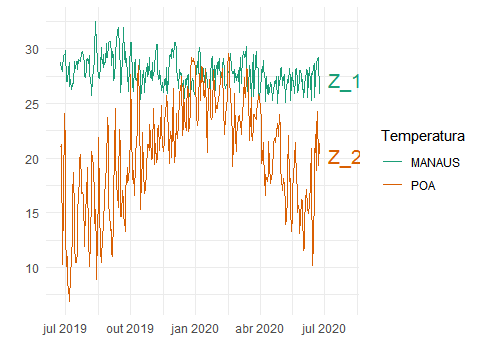
\includegraphics[width=0.9\linewidth]{02-SeriesReg_files/figure-latex/figts1-1} 

}

\caption{Temperaturas médias diárias nas cidades de Manaus (MA) e Porto Alegre (POA)}\label{fig:figts1}
\end{figure}

Cada curva do gráfico é chamada de trajetória ou série temporal ou função amostral. No gráfico acima \(Z_{(j)}(t)\) é o valor da temperatura no instante \(t\), para a \(j\)-ésima trajetória (\(j\)-ésimo ponto de observação). Para cada \(t\) fixo, teremos os valores de uma variável aleatória \(Z(t)\) que terá certa distribuição de probabilidade. Na realidade o que chamamos de série temporal, é uma parte de uma trajetória, dentre muitas que poderiam ter sido observadas. O parâmetro \(t\) pode ser função de algum outro parâmetro físico como por exemplo: espaço e volume.

\hypertarget{regressuxe3o-com-dados-de-suxe9ries-temporais}{%
\section{Regressão com dados de séries temporais}\label{regressuxe3o-com-dados-de-suxe9ries-temporais}}

Nesta seção estudaremos modelos de regressão cujas variáveis são séries temporais. O interesse principal recai sobre as condições necessárias para que o estimador de MQO apresente boas propriedades.

\hypertarget{diferenuxe7a-entre-dados-de-suxe9ries-temporais-e-dados-de-corte-transversal}{%
\subsection{Diferença entre dados de séries temporais e dados de corte transversal}\label{diferenuxe7a-entre-dados-de-suxe9ries-temporais-e-dados-de-corte-transversal}}

A primeira diferença entre dados de séries temporais e dados de corte transversal é que uma série temporal tem uma ordenação temporal. Outra característica, é que não temos mais independência entre as observações, ou seja, não temos mais uma amostra aleatória de indivíduos. Logo, para estimar um modelo do tipo
\begin{equation}
 y_t = \beta_0 + \beta_1 + \beta_2 x_{t1}+ x_{t2} + \ldots+\beta_k x_{tk}+ u_t,
 \label{eq:eq1STR}
\end{equation}
são necessárias novas suposições para que o estimador de MQO tenha boas propriedades.

\hypertarget{modelos-de-regressuxe3o-de-suxe9ries-temporais}{%
\subsection{Modelos de regressão de séries temporais}\label{modelos-de-regressuxe3o-de-suxe9ries-temporais}}

\hypertarget{modelos-estuxe1ticos}{%
\subsubsection{Modelos estáticos}\label{modelos-estuxe1ticos}}

Suponha que temos dados de séries temporais disponíveis para duas variáveis, digamos \(y\) e \(z\), em que \(y_t\) e \(z_t\) são datadas contemporaneamente. Um modelo que relaciona \(y\) a \(z\) é:
\begin{equation}
y_t = \beta_0 + \beta_1 z_t + u_t,  \,\,\,\,t=1,2,\ldots,n.
\label{eq:modelstatic}
\end{equation}
O nome ``Modelo Estático'' deriva do fato de relacionar as variáveis de forma contemporânea.

\begin{example}
\protect\hypertarget{exm:exampcurvphilips}{}{\label{exm:exampcurvphilips} }Um exemplo de modelo estático é a \textbf{curva de Phillips estática}, representada por:
\begin{equation}
inf_t = \beta_0 + \beta_1 desemp_t + u_t,
\label{eq:philcurve}
\end{equation}
em que \(inf_t\) é a inflação anual e \(desemp_t\) é a taxa de desemprego.
\end{example}

Este modelo é usado para estudar a relação de trocas contemporânea entre \(inf_t\) e \(desemp_t\) pressupondo uma \emph{taxa natural de desemprego} e expectativas inflacionárias constantes.

\hypertarget{modelos-de-defasagem-distribuuxedda-finita}{%
\subsection{Modelos de defasagem distribuída finita}\label{modelos-de-defasagem-distribuuxedda-finita}}

Em um \emph{modelo de defasagem distribuída finita} (MDD) permite-se que uma ou mais variáveis
afetem \(y\) com defasagens
\begin{equation}
y_t = \alpha_0 + \delta_0 z_t+\delta_1 z_{t-1} + \delta_2 z_{t-2} + u_t,
\label{eq:eqmdd2}
\end{equation}
que é um MDD de \emph{ordem 2}. De modo mais geral, um modelo de defasagem distribuída de ordem \(q\) incluirá \(q\) defasagens de \(z\).

Para interpretar os coeficientes em \eqref{eq:eqmdd2} suponha que \(z\) seja constante igual a \(c\),
em todos os períodos de tempo antes de \(t\) (\ldots, \(z_{t-2}=c\), \(z_{t-1}=c\)). Em \(t\), \(z\) aumenta em uma unidade, ou seja, \(z_t=c+1\), e, em seguida, retorna ao seu nível anterior em \(t+1\), isto é, \(z_{t+1}=c\).

Para enfatizar o efeito \emph{ceteris  paribus} de \(z\) sobre \(y\), suponhamos que o termo de erro em cada período seja zero. Então,
\begin{eqnarray*}
y_{t-1}&=&\alpha_0+\delta_0c+\delta_1c+\delta_2c\\
y_{t}&=&\alpha_0+\delta_0(c+1)+\delta_1c+\delta_2c\\
y_{t+1}&=&\alpha_0+\delta_0c+\delta_1(c+1)+\delta_2c\\
y_{t+2}&=&\alpha_0+\delta_0c+\delta_1c+\delta_2(c+1)\\
y_{t+3}&=&\alpha_0+\delta_0c+\delta_1c+\delta_2c,\\
\end{eqnarray*}
e assim por diante. Das duas primeiras equações temos
\begin{equation*}
y_t-y_{t-1} =\delta_0,
\end{equation*}
mostra que \(\delta_0\) é a mudança imediata em \(y\) em razão do aumento de uma unidade em \(z\) no tempo \(t\). Denomina-se \(\delta_0\) como \emph{propensão de impacto} ou \emph{multiplicador de impacto}.

Da mesma forma,
\begin{equation*}
\delta_1  =  y_{t+1} - y_{t-1},
\end{equation*}
é a mudança em \(y\) após a mudança temporária e
\begin{equation*}
\delta_2  =  y_{t+2} - y_{t-1},
\end{equation*}
é a mudança em \(y\) dois períodos após a mudança. Em \(t+3\), \(y\) retornou ao seu nível inicial \(y_{t+3}=y_{t-1}\). Isso ocorre porque presumimos que apenas duas defasagens de \(z\) aparecem em \eqref{eq:eqmdd2}.

Quando traçamos um gráfico de \(\delta_j\) como uma função de \(j\) obtemos a \emph{distribuição de defasagem}, que resume o efeito dinâmico que um aumento temporário em \(z\) tem em \(y\).

No entanto, o aumento em \(z\) pode ser permanente. Suponhamos que antes do tempo \(t\) \(z\) é constante igual a \(c\), ou seja, \(z_s=c\), para \(s<t\), e no tempo \(t\), \(z\) sofre um aumento permanente de uma unidade no tempo \(t\), ou seja, \(z_s=c+1\) para \(s\geq t\). Novamente, fazendo os erros iguais a zero, temos
\begin{eqnarray*}
y_{t-1}&=&\alpha_0+\delta_0c+\delta_1c+\delta_2c\\
y_{t}&=&\alpha_0+\delta_0(c+1)+\delta_1c+\delta_2c\\
y_{t+1}&=&\alpha_0+\delta_0(c+1)+\delta_1(c+1)+\delta_2c\\
y_{t+2}&=&\alpha_0+\delta_0(c+1)+\delta_1(c+1)+\delta_2(c+1)\\
\end{eqnarray*}
e assim por diante. Com o aumento permanente em \(z\), depois de um período \(y\) aumentou \(\delta_0+\delta_1\), e depois de dois períodos, \(y\) aumentou \(\delta_0+\delta_1+\delta_2\). Isso mostra que a soma dos coeficientes de \(z\) atual e defazadas,
\begin{equation}
 \delta_0+\delta_1+\delta_2
 \label{eq:eqPLP2}
\end{equation}
é a \emph{mudança de  longo prazo} em \(y\) quando há um aumento permanente em \(z\). A equação \eqref{eq:eqPLP2} é chamada \emph{propensão  de longo prazo (PLP)}.

A generalização para \(q\) defasagens é imediata.

\hypertarget{suposiuxe7uxf5es-para-modelos-com-suxe9ries-temporais}{%
\section{Suposições para modelos com séries temporais}\label{suposiuxe7uxf5es-para-modelos-com-suxe9ries-temporais}}

Nesta seção o objetivo é mostrar como as hipóteses clássicas devem ser alteradas
para cobrir regressão de séries temporais.

\hypertarget{inexistuxeancia-de-viuxe9s-do-mqo}{%
\subsection{Inexistência de viés do MQO}\label{inexistuxeancia-de-viuxe9s-do-mqo}}

Para que as estimativas via MQO dos parâmetros de um modelo de regressão com séries temporais não sejam viesadas são necessárias a seguintes hipóteses:

\begin{quote}
\textbf{\emph{Suposição TS.1:}} \emph{(linearidade nos parâmetros)}.
O processo estocástico
\[\{(x_{t1}, x_{t2},\ldots, y_t):\,\,\, t = 1, 2,\ldots, n\}\]
segue o modelo linear:
\[y_t = \beta_0 + \beta_1 x_{t1} + \cdots + \beta_k x_{tk}+u_t,\]
em que \(\{u_t:\,\,\,t=1,2,\ldots,n\}\) é a sequência de erros ou perturbações.
\end{quote}

\begin{quote}
\textbf{\emph{Suposição TS.2:}} \emph{(Inexistência  de colineariedade Perfeita)}. Na amostra, nenhuma das variáveis independentes é constante ou combinação linear perfeita das outras.
\end{quote}

As hipóteses \textbf{TS.1} e \textbf{TS.2} são essencialmente as mesmas daquelas usadas no contexto de
dados de cortes transversais.

\begin{quote}
\textbf{\emph{Suposição TS.3:}} \emph{(Média condicional zero ou exogeneidade estrita)}. O termo de erro em qualquer dado período é não correlacionado com as variáveis explicativas em todos os períodos de tempo, ou seja \(\mathbb{E} (u_t | X) = 0\), para \$ t = 1, 2,\ldots, n\$.
\end{quote}

Analisando-se a hipótese TS.3, percebemos que ela difere da hipótese clássica.
Observe que a hipótese TS.3 exige que o erro no tempo \(t\), \(u_t\) seja não correlacionado
com cada variável explicativa em \emph{todos} os períodos de tempo.

Se em termos de média condicional, temos somente a condição de não correlação somente no tempo
\(t\), da forma
\begin{equation}
\mathbb{E}(u_t|x_{1t},\ldots,x_{tk})=\mathbb{E} (u_t | X_t) = 0,
\label{eq:exoc}
\end{equation}
diz-se que vale a \emph{exogeneidade contemporânea} das variáveis explicativas. Exogeneidade contemporânea só será suficiente em grandes amostras.
\eqref{eq:exoc}

A hipótese \textbf{TS.3} é muito forte e muitas vezes não verificada. Nos seguintes exemplos podemos ver como ela pode ser verificada na prática.

\begin{example}
\protect\hypertarget{exm:examphomic}{}{\label{exm:examphomic} }Suponha que a taxa de homicídios (\(homi_t\)) em uma cidade em termos do número de policiais per capita (\(polpc_t\))
\[homi_t = \beta_0 + \beta_1 polpc_t + u_t.\]

O termo de erro \(u\) precisaria ser não correlacionados com os valores atuais,os valores passados e futuros de \(polpc_t\). Podemos aceitar que \(u\) não é correlacionado com valores corrente e valores passados do regressor. Mas é evidente que um aumento em \(u\) hoje, provavelmente, levará a políticas que tentem aumentar \(polpc_t\) no futuro. Logo \textbf{TS.3} falha.
\end{example}

Quando \(u\) é correlacionado com o passado dos regressores, podemos resolver o problema incluindo defasagens dos regressores e utilizando um modelo de defasagem distribuída. Mas não podemos ter, de forma alguma, a influência de \(u\) no futuro dos regressores.

\begin{theorem}
\protect\hypertarget{thm:teovies}{}{\label{thm:teovies} } Sob as Hipóteses \textbf{ST.1}, \textbf{ST.2} e \textbf{ST.3} os estimadores de MQO são não viesados condicionados a \(X\) e, portanto, também incondicionalmente:
\begin{equation*}
   \mathbb{E}(\hat{\beta}_j)=\beta_j, \,\,\,j=1,\ldots,k.
 \end{equation*}
\end{theorem}

\hypertarget{variuxe2ncia-dos-estimadores-mqo}{%
\subsection{Variância dos estimadores MQO}\label{variuxe2ncia-dos-estimadores-mqo}}

É necessário mais duas hipóteses para completar o conjunto de hipóteses de Gauss-Markov para
regressões de séries temporais. A primeira delas é familiar da análise de corte transversal.

\begin{quote}
\textbf{\emph{Suposição TS.4:}} \emph{(Homoscedasticidade)}. Condicional a \(X\), a variância de \(u_t\) é a mesma para todo \(t\):
\[Var(u_t | X) = Var(u_t)=\sigma^2,\] para \$ t = 1, 2,\ldots, n\$.
\end{quote}

\begin{quote}
\textbf{\emph{Suposição TS.5:}} \emph{(Inexistência de Correlação Serial)}.
Condicional a \(X\), os erros em dois períodos de tempos diferentes são não correlacionados:
\[Corr(u_t ,u_s| X) =0,\] para todo \$ t \neq s\$.
\end{quote}

Com este conjunto de condições podemos enunciar o teorema de Gauss-Markov no contexto de séries temporais.

\begin{theorem}[Teorema de Gauss-Markov]
\protect\hypertarget{thm:teogm}{}{\label{thm:teogm} \iffalse (Teorema de Gauss-Markov) \fi{} }Sob as Hipóteses \textbf{ST.1} a \textbf{ST.5} os estimadores de MQO são os melhores estimadores lineares não viesados condicionais a \(X\), ou seja, são \textbf{\emph{BLUE}}.
\end{theorem}

\hypertarget{inferuxeancia-sob-as-hipuxf3teses-do-modelo-linear-cluxe1ssico}{%
\subsection{Inferência sob as hipóteses do modelo linear clássico}\label{inferuxeancia-sob-as-hipuxf3teses-do-modelo-linear-cluxe1ssico}}

Para que sejam válidos os testes \(t\), \(F\) e outros testes estatísticos baseadas nos erros padrões é necessário adicionar mais uma hipótese a respeito da distribuição dos erros. Esta hipótese é análoga à hipótese de normalidade usada para análise de corte transversal.

\begin{quote}
\textbf{\emph{Suposição TS.6:}} \emph{(Normalidade)}. Os erros \(u_t\) são independentes de \(X\) e são i.i.d. com distribuição normal com média zero e variância \(\sigma^2\)
\[u_t\sim\mathcal{N}(0,\sigma^2),\] para \$ t = 1, 2,\ldots, n\$.
\end{quote}

\begin{theorem}
\protect\hypertarget{thm:teoinfmqo}{}{\label{thm:teoinfmqo} }Sob as hipóteses \textbf{TS.1} a \textbf{TS.6}, as hipóteses do modelo linear clássico para séries temporais, os estimadores MQO são normalmente distribuídos, condicional em \(X\). Além disso, a estatística \(t\) tem uma distribuição \(t\), e cada estatística \(F\) tem uma distribuição \(F\).
\end{theorem}

\hypertarget{tenduxeancia}{%
\subsection{Tendência}\label{tenduxeancia}}

Quando trabalhamos com séries temporais é necessário saber reconhecer se estas séries contém uma tendência temporal. Ignorar o fato de que duas séries temporais podem ser correlacionadas somente porque ambas estão apresentando uma mesma tendência ao longo do tempo, em vez de uma relação causal, pode levar a conclusões errôneas e a possibilidade de uma regressão espúria. Vejamos o exemplo de uma série temporal com tendência temporal:

\begin{Shaded}
\begin{Highlighting}[]
\CommentTok{#library(readxl)}
\CommentTok{#library(ggplot2)}
\CommentTok{# Dados baixados em 25/06/2020 de}
\CommentTok{# https://seriesestatisticas.ibge.gov.br/series.aspx?vcodigo=PRECO415&t=custo-medio-m2}

\NormalTok{custo_medio <-}\StringTok{ }\KeywordTok{read_excel}\NormalTok{(}\StringTok{"Dados/custo_medio_m2.xls"}\NormalTok{)}
\KeywordTok{ggplot}\NormalTok{(custo_medio, }\KeywordTok{aes}\NormalTok{(}\DataTypeTok{x =}\NormalTok{ data, }\DataTypeTok{y =}\NormalTok{ cm)) }\OperatorTok{+}\StringTok{ }
\StringTok{  }\KeywordTok{geom_line}\NormalTok{()}\OperatorTok{+}\StringTok{ }\KeywordTok{theme_light}\NormalTok{()}\OperatorTok{+}\KeywordTok{labs}\NormalTok{( }\DataTypeTok{x=}\StringTok{""}\NormalTok{, }\DataTypeTok{y=}\StringTok{"Custo médio"}\NormalTok{)}
\end{Highlighting}
\end{Shaded}

\begin{figure}

{\centering 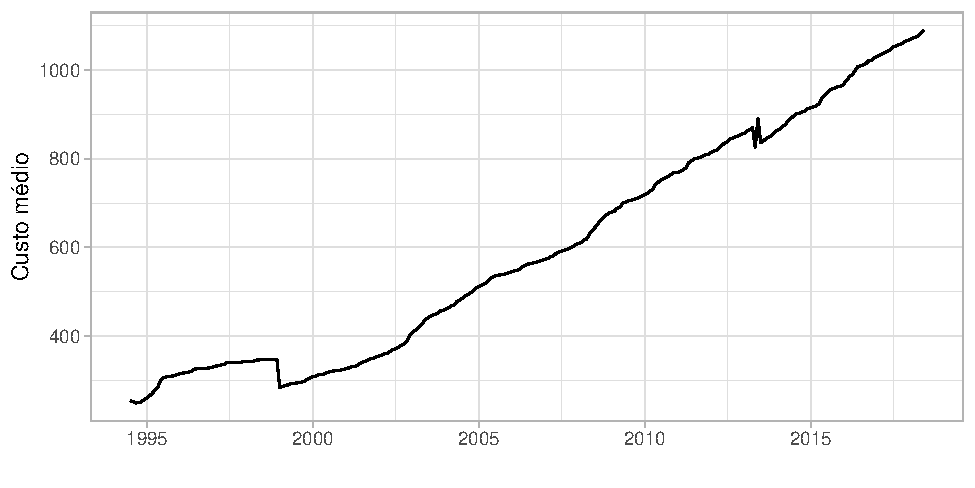
\includegraphics[width=0.65\linewidth]{02-SeriesReg_files/figure-latex/figcn-1} 

}

\caption{Custo médio do $m^2$ no Brasil a partir do plano real}\label{fig:figcn}
\end{figure}

Um modelo que captura tendência temporal é:
\begin{equation}
y_t = \alpha_0+ \alpha_1t + e_t, \hspace{1cm} t = 1, 2, \ldots,
\label{eq:tendmodel}
\end{equation}
em que assume-se que \(\{e_t\}\) é i.i.d. com \(\mathbb{E}(e_t)=0\) e \(\mbox{Var}(e_t)=\sigma^2\).
Observe que o parâmetro \(\alpha_1\) multiplica o tempo, resultando em uma \emph{tendência temporal linear}. Assim, \(\alpha_1\) mede a mudança em \(y_t\), de um período para o próximo, motivado pela passagem do tempo, mantendo-se todos os outros fatores fixos.

Outros modelos podem ser usados para capturar tendências temporais, dependendo da situação.
No modelo em que o logaritmo natural de \(y_t\) (presumindo que \(y_t>0\)) apresenta uma tendência temporal linear,

\begin{equation}
\log(y_t) = \beta_0+ \beta_1t + e_t, \hspace{1cm} t = 1, 2, \ldots,
\label{eq:logtend}
\end{equation}
diz-se que \(y_t\) tem uma \textbf{\emph{tendência exponencial}}.

Outra possibilidade é que em vez de uma tendência temporal linear, poderíamos ter uma
\textbf{\emph{tendência temporal quadrática}},

\begin{equation}
y_t = \beta_0+ \beta_1t +\beta_t^2+ e_t, \hspace{1cm} t = 1, 2, \ldots.
\label{eq:quadtend}
\end{equation}

\hypertarget{usando-variuxe1veis-de-tenduxeancia-na-anuxe1lise-de-regressuxe3o}{%
\subsection{Usando variáveis de tendência na análise de regressão}\label{usando-variuxe1veis-de-tenduxeancia-na-anuxe1lise-de-regressuxe3o}}

Suponha que existam dois fatores observados, \(x_{t1}\) e \(x_{t2}\) que afetam \(y_t\). Além disso,
existem fatores não observados que estão sistematicamente crescendo ou decrescendo ao longo do tempo.
Um modelo que captura isso é:
\begin{equation}
y_t = \beta_0 + \beta_1x_{t1} + \beta_2x_{t2} + \beta_3t + u_t.
\label{eq:tr2}
\end{equation}
Permitindo uma tendência temporal no modelo, reconhece-se que \(y_t\) pode estar crescendo
ou decrescendo ao longo do tempo por razões essencialmente não relacionadas a \(x_{t1}\) e \(x_{t2}\).

A omissão da variável \(t\) pode levar ao viés por omissão de variável, especialmente se \(x_{t1}\) ou \(x_{t2}\) apresentarem algum tipo de tendência, pois elas podem ser altamente correlacionadas com \(t\).

Adicionando um termo de tendência linear em um modelo de regressão é a mesma coisa que usar
série ``destendenciada'' numa regressão. Os estimadores \(\beta_1\) e \(\beta_2\) do modelo \eqref{eq:tr2} podem ser obtidos através de um procedimento de ``remoção da tendência temporal'' das séries originais:

Destendenciar uma série envolve regredir cada variável do modelo em \(t\) e uma constante (no caso de \eqref{eq:tr2}, regredir \(y_t\), \(x_{t1}\) e \(x_{t2}\) contra \(t\) e uma constante).

Os resíduos destas regressões, \(\ddot{y}_t\), \(\ddot{x}_{t1}\) e \(\ddot{x}_{t2}\), constituem uma série temporal sem tendência.

Em seguida, realizar a regressão com variáveis retificada,
\begin{equation}
\ddot{y}_t= \delta_1\ddot{x}_{t1}+\delta_2\ddot{x}_{t2}+v,
\label{eq:varrat}
\end{equation}
(não precisa intercepto, será igual a 0). As estimativas via MQO, \(\hat{\delta}_1\) e \(\hat{\delta}_2\) serão iguais as estimativas \(\hat{\beta}_1\) e \(\hat{\beta}_2\) da regressão \eqref{eq:tr2}.

\hypertarget{sazonalidade}{%
\section{Sazonalidade}\label{sazonalidade}}

Sazonalidade ocorre quando uma série exibe comportamentos semelhantes em determinados períodos. Um exemplo é o **Índice de produção física industrial de bens intermediários*. O objetivo do índice é servir como uma medida aproximada da evolução de curto prazo do valor adicionado da indústria, dado um determinado período de referência (base: média de 2012).

\begin{Shaded}
\begin{Highlighting}[]
\CommentTok{#library(readxl)}
\CommentTok{#library(plotly)}
\CommentTok{#Fonte: "IBGE - Pesquisa Industrial Mensal - Produção Física"}
\NormalTok{prodind <-}\StringTok{ }\KeywordTok{read_excel}\NormalTok{(}\StringTok{"Dados/ProducaoIndustrial.xls"}\NormalTok{)}
\KeywordTok{ggplot}\NormalTok{(prodind,}\KeywordTok{aes}\NormalTok{(}\DataTypeTok{x=}\NormalTok{Data, }\DataTypeTok{y=}\NormalTok{intermediarios))}\OperatorTok{+}
\StringTok{  }\KeywordTok{geom_line}\NormalTok{(}\DataTypeTok{col=}\StringTok{"#D95F02"}\NormalTok{)}\OperatorTok{+}
\StringTok{  }\KeywordTok{labs}\NormalTok{(}\DataTypeTok{x =} \StringTok{""}\NormalTok{,}\DataTypeTok{y=}\StringTok{"Índice"}\NormalTok{)}\OperatorTok{+}
\StringTok{  }\KeywordTok{theme_minimal}\NormalTok{()}
\end{Highlighting}
\end{Shaded}

\begin{figure}

{\centering 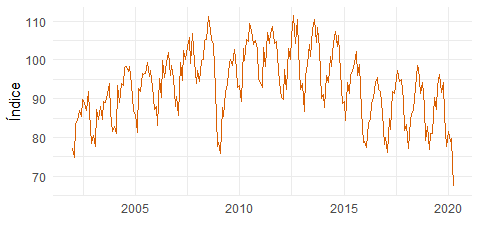
\includegraphics[width=0.85\linewidth]{02-SeriesReg_files/figure-latex/figpi-1} 

}

\caption{Produção física industrial de Bens Intermediários}\label{fig:figpi}
\end{figure}

É comum que as séries de dados mensais e trimestrais exibam padrões sazonais, mas isso não é uma regra. Por exemplo, não existe padrão sazonal observável nas taxas de juros ou de inflação. Além disso, séries que exibem padrões sazonais são \textbf{\emph{ajustadas sazonalmente}} antes de serem informadas para o público.

Uma série ajustada sazonalmente é a série que teve os fatores sazonais removidos. Existem vários métodos para isso. Um dos métodos mais simples é incluir um conjunto de variáveis dummies sazonais. Seja o seguinte modelo para dados mensais:

\begin{equation}
y_t = \beta_0 + \delta_1fev_t + \delta_2mar_t + \cdots + \delta_{11}dez_t + \beta_1x_{t1} +\cdots + \beta_kx_{tk} + u_t.
\label{eq:saz1}
\end{equation}
em que \(fev_t,mar_t,\cdots,dez_t\) são variáveis dummy indicando se o período de tempo \(t\) correspondo ao mês apropriado. Nesta formulação, janeiro é o mês-base e \(\beta_0\) seu intercepto. Se colocarmos janeiro no modelo e um intercepto, teremos um problema de multicolineariedade.

Se não existir sazonalidade em \(y_t\), dado que controlamos os regressores \(x_{tj}\), então
os coeficientes \(\delta_1;\ldots; \delta_{11}\) devem ser todos iguais a zero, o que pode ser testado através de um teste \(F\).

Considere o modelo \eqref{eq:saz1}, para \(k = 2\), ou seja 2 regressores. Podemos obter os seus estimadores, \(\hat{\beta}_1\) e \(\hat{\beta}_2\), através do seguinte procedimento:

Regrida a variável dependente, e cada um dos regressores, separadamente, contra
uma constante e as dummies mensais e guarde os resíduos, digamos \(\ddot{y}_t\), \(\ddot{x}_{t1}\) e \(\ddot{x}_{t2}\).

Por exemplo,
\begin{equation*}
\ddot{y}_t = y_t-\hat{\alpha}_0 - \hat{\alpha}_1fev_t - \hat{\alpha}_2mar_t -\cdots - \hat{\alpha}_{11}dez_t.
\end{equation*}
Este é o método para dessazonalizar uma série temporal mensal.

Roda a regressão de \(\ddot{y}_t\) contra \(\ddot{x}_{t1}\) e \(\ddot{x}_{t2}\) sem as dummies mensais.

\hypertarget{processos-de-covariuxe2ncia-estacionuxe1ria}{%
\subsection{Processos de covariância estacionária}\label{processos-de-covariuxe2ncia-estacionuxe1ria}}

Um processo estocástico é covariância estacionária se \(\mathbb{E} (x_t)\) é constante, \(\mbox{Var}(x_t)\) é constante e para qualquer \(t, h\geq 1\), \(\mbox{Cov}(x_t,x_{t + h})\) depende apenas em \(h\), e não em \(t\). Mais adiante abordaremos essa definição com maior profundidade.

\hypertarget{processos-fracamente-dependente}{%
\subsection{Processos fracamente dependente}\label{processos-fracamente-dependente}}

Uma série temporal estacionária é fracamente dependente se \(x_t\) e \(x_{t + h}\) são
``quase independentes'', quando \(h\) aumenta.

Se, para um processo de covariância estacionária \(\mbox{Cor}(x_t, x_{t + h})\rightarrow 0\) quando \(h\rightarrow \infty\), dizemos que este processo de covariância estacionária é fracamente dependente.

Essa definição é necessária para usar \emph{Leis dos Grandes Números} e \emph{Teorema Central do Limite}.

\begin{example}
\protect\hypertarget{exm:Wpg365}{}{\label{exm:Wpg365} }MA(1) pg 356 Wooldridge.
\end{example}

\begin{example}
\protect\hypertarget{exm:Wpg366}{}{\label{exm:Wpg366} }Exemplo: AR(1) pg 356 Wooldridge.
\end{example}

\newpage

\hypertarget{exercuxedcios}{%
\section{Exercícios}\label{exercuxedcios}}

\begin{exercise}
\protect\hypertarget{exr:exsr1}{}{\label{exr:exsr1} }Sobre regressão com séries temporais responda:

~~~a) Quais as principais diferenças entre dados transversais e séries temporais?\\
\hspace*{0.333em}\hspace*{0.333em}\hspace*{0.333em}b) Explique o que é exogeneidade contemporânea e exogeneidade estrita.

~~~c) Comente sobre a diferença entre homocedasticidade e correlação serial.

~~~d) A suposição de normalidade dos erros é necessária para se obter estimadores consistentes via MQO? Qual é o objetivo ao se fazer uma suposição para distribuição dos erros?
\end{exercise}

\begin{exercise}[anpec-2010]
\protect\hypertarget{exr:exsr2}{}{\label{exr:exsr2} \iffalse (anpec-2010) \fi{} }Considere o modelo de regressão linear múltipla com regressores estocásticos \(y_t = \beta_1 x_{1t} + \beta_2 x_{2t} + \varepsilon_t\), no qual \(\varepsilon_t\) não é autocorrelacionado e tem média e variância condicionais a \(x_{1t}\) e \(x_{2t}\) iguais a zero e \(s^2\), respectivamente. Por simplicidade, suponha que as variáveis são expressas como desvios com relação às respectivas médias.

Responda:

~~~a) Se \(\beta_2 = 0\) e incluirmos \(x_{2t}\) na regressão, o estimador de mínimos quadrados ordinários de \(\beta_1\) será viesado?

~~~b) Se não conseguirmos observar \(x_{1t}\), mas apenas \(x_{1t}^*=x_{1t}+u_t\), em que \(u_t\) é um erro de medida, e se substituirmos \(x_{1t}\) por \(x_{1t}\) na regressão, o estimador de mínimos quadrados ordinários de \(\beta_1\) ainda assim será consistente?

~~~c) Se \(x_{2t} = y_{t-1}\) e relaxarmos a hipótese de que os erros \(\varepsilon_t\)`s não são autocorrelacionados, o estimador de mínimos quadrados ordinários de \(\beta_2\) será consistente, porém não será eficiente?

~~~d) Seja \(c\) uma constante diferente de zero. Defina \(\tilde{y}= cy_t\), \(\tilde{x}_{1t}= cx_{1t}\) e \(\tilde{x}_{2t} = cx_{2t}\). Os estimadores de mínimos quadrados ordinários (MQO) em uma regressão de \(\tilde{y}\) contra \(\tilde{x}_{1t}\) e \(\tilde{x}_{2t}\) coincidem com os estimadores de MQO em uma regressão de \(y_t\) contra \(x_{1t}\) e \(x_{2t}\)?

~~~e) A variância do estimador de mínimos quadrados ordinários diverge para infinito à medida que a correlação entre \(x_{1t}\) e \(x_{2t}\) aproxima-se de 1;

~~~f) Denote por \(\widehat{\varepsilon}_t\) o resíduo da regressão de mínimos quadrados ordinários. A hipótese de que o erro é correlacionado com \(x_{1t}\) pode ser testada utilizando a estatística \(\frac{1}{T}\sum_{i=1}^{T}x_{1i}\widehat{\varepsilon}_{i}\)?
\end{exercise}

\begin{exercise}
\protect\hypertarget{exr:exsr3}{}{\label{exr:exsr3} }Em uma equação de dados anuais, supondo que
\[jur_t=1,6+0,48inf_t-0,15inf_{t-1}+0,32inf_{t-2}+u_t,\]
em que \(jur\) é a taxa de juros e \(inf\) é a taxa de inflação.

~~~a) Supondo válida a hipótese de exogeneidade estrita, como deve ter sido estimado o modelo acima? Justifique?\\
\hspace*{0.333em}\hspace*{0.333em}\hspace*{0.333em}b) Qual é o efeito de curto prazo (propensão de impacto) da taxa de inflação sobre a taxa juros? Qual é o efeito de longo prazo da taxa de inflação sobre a taxa de juros?
\end{exercise}

\begin{exercise}
\protect\hypertarget{exr:exsr4}{}{\label{exr:exsr4} }Considere uma série temporal de 10 anos contendo PIB (em R\$ ) e número de homicídios (em unidades) em um determinado país. O primeiro modelo estimado foi \(pib_t=\beta_0+\beta_1homic_t+u_t\). Os resultados da estimação se encontram na tabela 1. Um segundo modelo foi \(pib_t=\beta_0+\beta_1homic_t+\beta_2t+u_t\), em que \(t\) é um termo de tendência. Os resultados da estimação desse modelo se encontram na tabela 2:

\begin{longtable}[]{@{}lllll@{}}
\toprule
Tabela 1 & Estimate & Std. Error & t-value & Pr(\textgreater{}\tabularnewline
\midrule
\endhead
(Intercept) & -3461194.26 & 314948.06 & -10.99 & 0.00\tabularnewline
homic & 102.63 & 6.12 & 16.76 & 0.00\tabularnewline
\bottomrule
\end{longtable}

\begin{longtable}[]{@{}lllll@{}}
\toprule
Tabela 2 & Estimate & Std. Error & t-value & Pr(\textgreater{}\tabularnewline
\midrule
\endhead
(Intercept) & 5564710.45 & 2539866.04 & 2.19 & 0.06\tabularnewline
homic & -123.64 & 63.59 & -1.94 & 0.09\tabularnewline
t & 423054.01 & 118647.95 & 3.57 & 0.01\tabularnewline
\bottomrule
\end{longtable}

~~~a) O coeficiente de \(homic\) é significativo no primeiro modelo a 5\% de significância? Interprete o valor desse coeficiente.

~~~b) O coeficiente de \(homic\) é significativo no segundo modelo a 5\% de significância? Interprete o valor desse coeficiente.

~~~c) O coeficiente de \(t\) é significativo no segundo modelo a 5\% de significância? Interprete o valor desse coeficiente.

~~~d) Explique o resultado (surpreendente) encontrado no primeiro modelo, ressaltando a importância do procedimento adotado no segundo modelo.
\end{exercise}

\begin{exercise}
\protect\hypertarget{exr:exsr5}{}{\label{exr:exsr5} }Considere uma série do PIB brasileiro com início no primeiro trimestre 1996 e fim no segundo bimestre de 2010. Essa série foi decomposta em sua tendência \((t)\) e variáveis dummy para a sazonalidade, em que \(S_i = 1\), se a observação pertence ao trimestre \(i\) e \(S_i = 0\), caso contrário.

~~~a) Se tentarmos estimar o modelo \(pib_t=\beta_0+\beta_1S_1+\beta_2S_2+\beta_3S_3+\beta_4S_4+\gamma t+u_t\), qual problema encontraremos? Explique porque isso ocorre.

~~~b) No modelo \(pib_t=\beta_1S_1+\beta_2S_2+\beta_3S_3+\beta_4S_4+\gamma t+u_t\), o que mede cada um dos \(\beta\)`s?

~~~c) No modelo \(pib_t=\beta_0+\beta_2S_2+\beta_3S_3+\beta_4S_4+\gamma t+u_t\), o que mede \(\beta_2\)?

~~~d) No modelo \(pib_t=\beta_0+\gamma t+\beta_2S_2+\beta_3S_3+\beta_4S_4+u_t\), foi estimado e apresentou a seguinte tabela ANOVA (Tabela 3). Faça um teste F para a hipótese nula de que não há sazonalidade. Use

\(\alpha=5\%\)

\begin{longtable}[]{@{}llll@{}}
\toprule
Tabela 3 & Df & Sum Sq & Mean Sq\tabularnewline
\midrule
\endhead
t & 1 & 2287298699531.79 & 2287298699531.79\tabularnewline
s2 & 1 & 1216754395.49 & 1216754395.49\tabularnewline
s3 & 1 & 31129772.60 & 31129772.60\tabularnewline
s4 & 1 & 5037536508.88 & 5037536508.88\tabularnewline
Residuals & 53 & 106216397798.70 & 2004082977.33\tabularnewline
\bottomrule
\end{longtable}
\end{exercise}

\begin{exercise}
\protect\hypertarget{exr:exsr6}{}{\label{exr:exsr6} }Considere o modelo \(y_t=\alpha_0+\delta_0z_t+\delta_1z_{t-1}+\delta_2z_{t-2}+u_t\).

~~~a) Por que devemos considerar a possibilidade de multicolinearidade nesse modelo?

~~~b) Reparametrize o modelo de modo a isolar o efeito de longo prazo como coeficiente da variável \(z_t\).

~~~c) Qual o benefício dessa reparametrização se estivermos interessados em testar a significância do efeito de LP da \(z\) sobre \(y\)?
\end{exercise}

\begin{exercise}
\protect\hypertarget{exr:exsr7}{}{\label{exr:exsr7} }Considere o seguinte modelo estático \(crime_t=\beta_0+\beta_1+pol_t+u_t\), em que \(crime_t\) é um índice de criminalidade no período \(t\) e \(pol_t\) é o número de policiais em \(t\).

~~~a) Supondo que \(pol\) seja estritamente exógeno na equação, como você estimaria \(\beta_0\) e \(\beta_1\). Quais as propriedades do estimador proposto em termos de viés e consistência?

~~~b) Suponha agora que o número de policiais em \(t\) seja definido em função do índice de criminalidade do período anterior. A hipótese de exogeneidade estrita continua válida? Justifique.
\end{exercise}

\begin{exercise}
\protect\hypertarget{exr:exsr8}{}{\label{exr:exsr8} }Um modelo de ajustamento parcial é dado por:
\[y^*_t=\beta_0+\beta_1x_t+e_t\]
\[y_t-y_{t-1}=\lambda(y^*_t-y_{t-1}),\]
em que \(y^*_t\) é o nível desejável ou ótimo de \(y\), e \(y_t\) é o nível efetivo (observado). Por exemplo, \(y^*_t\) é o crescimento desejável nos estoques de uma firma e \(x_t\) é o crescimento de vendas da firma. O parâmetro \(\lambda\) mede a
velocidade do ajustamento e satisfaz \(0 < \lambda < 1\).

~~~a) Insira a primeira equação na segunda equação e mostre que podemos escrever \(y_t=\alpha_0+\alpha_1 y_{t-1}+\alpha_2 x_t+u_t\). Quem são os \(\alpha\)s em termos dos \(\beta\)s e \(\lambda\)? Quem é \(u_t\) em termos de \(e_t\)?

~~~b) Supondo que \(\mathbb{E}(e_t|x_t,y_{t-1})=0\) e todas as séries sejam fracamente dependentes,

como você estimaria os \(\alpha\)s? É consistente? Justifique sua resposta. O estimador proposto é viciado?

~~~c) Seja \(\hat{\alpha}_1 = 0,7\) e \(\hat{\alpha}_2 = 0,2\).

\begin{verbatim}
(i) Qual o coeficiente de ajustamento estimado?

(ii) Qual o efeito de CP (curto prazo) de um crescimento das vendas da firma sobre o crescimento de estoques da firma?

(iii) Qual é o efeito de LP (longo prazo)?
\end{verbatim}
\end{exercise}

\begin{exercise}
\protect\hypertarget{exr:exsr9}{}{\label{exr:exsr9} }Imagine o seguinte modelo: \(Y_t = \beta_0 + \beta_1 X_t + u_t\) , onde \(Y\) é a demanda por moeda, \(X^*\) é a taxa de juros esperada no longo prazo e \(u\) é um termo de erro clássico, não correlacionado com \(X^*\). Como a variável de expectativa \(X^*\) não é diretamente observável, proporemos a seguinte hipótese para formação de expectativas (adaptativas): \(X^*_t- X^*_{t-1} = \gamma(X_t- X_{t-1} )\), em que \(\gamma\), tal que \(0 < \gamma < 1\), é conhecido como coeficiente de expectativas.

~~~a) Mostre que podemos escrever esse modelo como \(Y_t=\alpha_0+\alpha_1X_t+\alpha_2Y_{t-1}+v_t\). Quem são os \(\alpha\)s em termos dos \(\beta\)s e \(\gamma\)? Quem é \(v_t\) em termos de \(u_t\)?

~~~b) O que podemos dizer a respeito dos estimadores de MQO nesse caso? Justifique.

~~~c) Imagine que no modelo original \(u_t\) siga o esquema auto-regressivo de primeira ordem, i.e., \(u_t = \rho u_{t-1} + \varepsilon_t\), em que \(\rho\) é o coeficiente de autocorrelação e onde \(\varepsilon_t\) satisfaz as premissas clássicas. Se \(\rho=\lambda\), como você estimaria o modelo? Justifique.

~~~d) As estimativas obtidas no item anterior são não-viciadas? Consistentes? Justifique sua resposta.
\end{exercise}

\begin{exercise}
\protect\hypertarget{exr:exsr10}{}{\label{exr:exsr10} }Seja o processo \(y_t = e_t + \alpha_1 e_{t-1}\), em que \(e_t \sim iid(0,\sigma^2).\)

~~~a) Calcule \(\mathbb{E}(y_t )\), \(\mbox{Var}(y_t )\) e \(\mbox{Cov}(y_t , y_{t-h} )\), \(h = 1, 2, 3,\ldots\). O processo \(y_t\) é de covariância estacionária?

~~~b) Calcule as autocorrelações de primeira ordem e de segunda ordem para esse processo. Podemos dizer que o processo é fracamente dependente? Justifique.

~~~c) Faça o correlograma (gráfico da função de autocorrelação em função das defasagens) para esse processo.
\end{exercise}

\begin{exercise}
\protect\hypertarget{exr:exsr11}{}{\label{exr:exsr11} }Seja o processo \(y_t = c + \rho y_{t-1} + e_t\), em que \(e_t \sim iid(0,\sigma^2)\).

~~~a) Qual é a condição de estabilidade para esse processo? Calcule \(\mathbb{E}(y_t )\) e \(\mbox{Var}(y_t )\) considerando válida a condição de estabilidade.

~~~b) Para o processo \(y_t\) acima temos que \(\mbox{Cov}(y_t,y_{t-h} ) = \frac{\rho^h\sigma^2}{1-\rho^2}\), \(h = 1, 2, 3,\ldots\). O processo \(y_t\) é de covariância estacionária? Justifique.

~~~c) Calcule a autocorrelação de ordem \(h\) para o processo \(y_t\). Faça o correlograma até quatro defasagens para esse processo considerando \(\rho = 0,5\).
\end{exercise}

\hypertarget{st}{%
\chapter{Séries Temporais}\label{st}}

O estudo de séries temporais tem por objetivos principais definir o processo gerador de dados, fazer previsões futuras da série, identificar ciclos, tendências e/ou sazonalidades de forma que a decisão que envolve as variáveis em questão seja a mais acurada possível.

\hypertarget{objetivos}{%
\section{Objetivos}\label{objetivos}}

Na seção \ref{objetivos}

Dada uma série temporal \(\{Z(t_1 ),\ldots, Z(t_N)\}\), observada nos instantes \(t_1,\ldots,t_N\),
podemos estar interessados em:

~~~i) Investigar o mecanismo gerador da série temporal;

~~~ii) Fazer previsões de valores futuros da série; podendo ser a curto ou longo prazo;

~~~iii) Descrever apenas o comportamento da série através de gráficos;

~~~iv) Procurar periodicidades relevantes nos dados. Em todos estes casos podemos construir modelos probabilísticos ou estocásticos, tanto no domínio do tempo como no domínio da freqüência, por exemplo: um sinal aleatório com frequência medida em Hz. Devemos construir modelos simples e com menor número de parâmetros possíveis.

\hypertarget{suxe9ries-temporais-definiuxe7uxe3o-formal}{%
\section{Séries temporais: definição formal}\label{suxe9ries-temporais-definiuxe7uxe3o-formal}}

Neste capítulo vamos descrever os conceitos básicos utilizados dentro da teoria dos modelos de séries temporais. Inicialmente vamos introduzir os conceitos de processos estocásticos, média e função de covariância, processo estacionário e função de autocorrelação.

\hypertarget{processos-estocuxe1sticos}{%
\subsection{Processos estocásticos}\label{processos-estocuxe1sticos}}

Seja \(T\) um conjunto arbitrário de índices. Um \textbackslash textcolor\{blue\}\{\emph{processo estocástico}\} é uma família de variáveis aleatórias \(\{Z_t\}_{t \in T}\) definidas num mesmo espaço de probabilidades, que denotaremos genericamente por \((\Omega, \mathcal A, P)\). O conjunto de índices \(T\) pode ser o conjunto dos números inteiros \(\mathbb{Z} = \{0, \pm 1, \pm 2,\cdots\}\), dos naturais \(\mathbb{N}=\{1,2,\cdots\}\) ou o conjunto dos números reais \(\mathbb{R}\). Observe ainda que, para cada \(t \in T\), \(Z_t\) é uma variável aleatória definida sobre \(\Omega\), sendo assim de fato uma função de dois argumentos, do índice \(t\in T\) e do ponto \(\omega \in \Omega\) que determina o valor do processo no tempo \(t\) dado por \(Z_t(\omega)\).

Uma série temporal, do ponto de vista teórico, nada mais é do que um processo estocástico para o qual o índice \(T\) é \(\mathbb{Z}\) ou um subconjunto deste. Do ponto de vista prático porém, uma série temporal é um conjunto de dados indexados no tempo. Esta dualidade de nomenclatura será utilizado em todo o trabalho. Invariavemente, letras maiúsculas, como \(Z_1,Z_2,\cdots\) denotarão a série temporal do ponto de vista teórico, isto é, como variáveis aleatórias em um processo estocástico indexado pelo tempo, enquanto letras minúsculas como \(z_1,z_2,\cdots\) denotarão a série temporal do ponto de vista prático, isto é, como uma observação das variáveis aleatórias que compõem o processo estocástico. Assim, se do ponto de vista teórico temos a série temporal \(\{Z_t\}_{t\in\mathbb{Z}}\), um processo estocástico indexado pelo tempo, uma série temporal do ponto de vista prático significa uma realização \(z_1,\cdots,z_n\) do processo \(\{Z_t\}\), observados nos tempos \(t=1,\cdots,n\). Neste caso, observamos \(z_1=Z_1(\omega),\cdots, z_n=Z_n(\omega)\), para um determinado \(\omega\in\Omega\) fixo. Embora existam maneiras mais formais e precisas de definir uma série temporal, o ponto de vista aqui adotado, embora aparentemente ambíguo na nomenclatura, servirá bem a nossos propósitos sem causar confusões.

Chamamos atenção ainda que existem condições para que um processo estocástico exista. Estes resultados dependem de uma discussão bastante técnica, bem além das intenções de nossa exposição.

\hypertarget{especificauxe7uxe3o-de-um-processo-estocuxe1stico}{%
\subsection{Especificação de um processo estocástico}\label{especificauxe7uxe3o-de-um-processo-estocuxe1stico}}

Sejam \(t_1,t_2,\ldots,t_n\) elementos quaisquer de \(T\) e consideremos
\begin{equation}
F(Z_1,\ldots,Z_n; t_1,\ldots, t_n ) = P \{Z(t_1 )\leq z_1,\ldots, Z(t_n) \leq z_n \}
\label{eq:distfindim}
\end{equation}
então, o processo estocástico \(Z = \{Z(t), t \in T \}\) estará especificado se as distribuições
finito-dimensionais de \eqref{eq:distfindim}, são conhecidas para todo \(n\geq 1\).
Contudo, em termos práticos, não conhecemos todas essas distribuições finito-
dimensionais. Estudaremos então certas características associadas a \eqref{eq:distfindim} e que
sejam simples de calcular e interpretar. Uma maneira de especificar o processo \(Z\) seria determinar todos os produtos dos
momentos, ou seja,
\begin{equation}
\mu(r_1 ,\ldots, r_n; t_1,\ldots, t_n ) = \mathbb{E \,} Z^{r_1}(t_1 )\ldots Z^{r_n}(t_n)
\label{eq:prodmom}
\end{equation}
ou
\begin{equation}
\mu(\textbf{r},\textbf{t})=\int_{-\infty}^{\infty}\ldots\int_{-\infty}^{\infty}
                      Z^{r_1}_1\ldots Z^{r_n}_1 f(z_1,\ldots,z_n; t_1,\ldots,t_n)dz_1\ldots dz_n
\end{equation}
em que \(f(\textbf{Z},\textbf{t})\) é a função de densidade de \(F(\textbf{Z}, \textbf{t})\). Porém o que vai nos interessar são os momentos de baixa ordem, ou seja, os chamados processos estacionários de segunda ordem. Consideramos somente os momentos de primeira e segunda ordem, que serão apresentados a seguir.

\hypertarget{muxe9dias-e-covariuxe2ncias}{%
\section{Médias e covariâncias}\label{muxe9dias-e-covariuxe2ncias}}

Naturalmente, quando estamos trabalhando com um processo estocástico, cada variável aleatória que o compõe possui sua própria distribuição, assim como sua própria massa/densidade de probabilidade e sua própria média/variância. Para um processo estocástico \(\{Z_t\}_{t\in\mathbb{Z}}\) definimos, para cada \(t\in\mathbb{Z}\), a \textbackslash textcolor\{blue\}\{\emph{função média}\}, \(\mu_t\) e a \textbackslash textcolor\{blue\}\{\emph{função variância}\} \(\sigma^2_t\) respectivamente por

\begin{align}
\mu_t = \mathbb{E} (Z_t) \quad \mbox{ e }\quad \sigma_t^2=\mbox{Var}(Z_t),
\label{eq:funcmed}
\end{align}
desde que as esperanças envolvidas existam. Chamamos a atenção de que embora as esperanças e variâncias de um processo estocástico existam, estas podem ser infinitas. Este fato trás diversos problemas técnicos na análise de séries temporais e requerem técnicas avançadas de análise que estão fora do escopo deste trabalho. Por este motivo, neste trabalho assumiremos tacitamente que todos os processos estocásticos e variáveis aleatórias possuem esperança e variância finitas.

Outra estrutura importante relacionada a um processo estocástico é o que chamamos de estrutura de dependência do processo. Dependência entre variáveis aleatórias pode ser definida de diversas maneiras diferentes. Neste trabalho estamos especialmente interessados na estrutura de dependência relacionadas com a covariância e a correlação entre as variáveis do processo. Observe que num processo estocástico podemos definir a covariância e a correlação entre quaisquer pares \(Z_i\) e \(Z_j\) de variáveis, para \(i,j\in\mathbb{Z}\). No caso de processos, estas funções recebem o prefixo \emph{auto} para enfatizar o fato de que as covariâncias/correlações estão sendo calculadas entre as variáveis do processo. Definimos a
\textbackslash textcolor\{blue\}\{\emph{função de autocovariância}\}, abreviada \textbackslash textcolor\{blue\}\{\emph{FACV}\}, como

\begin{equation}
\gamma_Z(t,s) = \mbox{Cov}(Z_t , Z_s ) = E [(Z_t-\mu_t ) (Z_s-\mu_s )]=\mathbb{E} (Z_t Z_s ) - \mu_t \mu_s,\quad \mbox{ para }\quad t, s \in\mathbb{Z}.
\label{eq:funcacov}
\end{equation}

Analogamente. definimos a \textbackslash textcolor\{blue\}\{\emph{função de autocorrelação}\}, abreviada \textbackslash textcolor\{blue\}\{\emph{FAC}\}, por
\begin{equation}
\rho_Z(t,s) = \mbox{Cor}(Z_t , Z_s ) =\frac{\mbox{Cov}(Z_t , Z_s )}{\sqrt{\mbox{Var}(Z_t)\mbox{Var}(Z_s)}} = \frac{\gamma(t,s)}{\sqrt{\gamma(t,t)\gamma(s,s)}}.
\label{eq:funcfac}
\end{equation}
O subscrito ``\(Z\)'' nas definições acima são utilizados para reforçar à qual processo estamos nos referindo. Porém, quando não houver perigo de confusão, podemos eliminar a referência ao processo associado e escrever simplesmente \(\gamma(t,s)\) e \(\rho(t,s)\).

Observe que, em princípio, as funções \(\gamma(t,s)\) e \(\rho(t,s)\) dependem tanto de \(t\) quanto de \(s\). Nos casos em que isto acontece, qualquer tipo de inferência baseada em autocovariâncias/autocorrelações se torna impossível sem tomarmos medidas para tornar esta estrutura de dependência mais simples. Algumas técnicas relevantes para isso serão estudadas adiante. De qualquer forma, a teoria clássica de séries temporais lida com casos em que essas quantidades possuem uma dependência temporal simplificada, permitindo o seu estudo. Processos com estas características são de grande importância e serão estudados em detalhes mais adiante. Isto por que, do ponto de vista matemático, tal estrutura é conveniente e permite um tratamento rigoroso e aprofundado da teoria enquanto que do ponto de vista prático, é de fácil percepção, permite a modelagem, inferência, previsão e outros aspectos aplicados relevantes de maneira simples e rápida. Tudo isso contribuiu para a difusão de métodos baseado em autocovariâncias/autocorrelações.

\hypertarget{propriedades-importantes}{%
\subsection{Propriedades importantes}\label{propriedades-importantes}}

As seguintes propriedades da função de autocovariância e autocorrelação são análogas às da covariância e correlação ordinárias, mas merecem destaque. Para todo \(t,s\in\mathbb{Z}\), com \(t\neq s\),

~~~1) \(\gamma(t,t) = \mbox{Var}(Z_t)\), \quad  \(\rho(t,t) = 1;\)

~~~2) \(\gamma(t,s) = \gamma(s,t)\),\quad \(\rho(t,s) = \rho(s,t)\).

~~~3) \(|\gamma(t,s)|\leq \sqrt{\gamma(t,t)\gamma(s,s)}\),\quad \(-1 \leq \rho(t,s)\leq 1.\)

A propriedade 3 em particular mostra que a covariância entre duas variáveis está bem definida caso estas tenham variância finita.

Como sabemos a correlação é uma medida da dependência linear entre duas variáveis. Se \(\mbox{Cor}(X,Y)=\pm1\), isto significa que existem constantes \(\beta_0\) e \(\beta_1\) tais que \(Y=\beta_0+\beta_1X\). Ou seja, uma variável é exatamente uma função linear da outra. Valores próximos de \(\pm 1\) indicam forte dependência (linear) e valores próximos de 0 indicam fraca dependência (linear). Se \(\rho(t,s) = 0\), \(Z_t\) e \(Z_s\) são ditas não-correlacionadas, mas note que isso não quer dizer que elas são necessariamente independentes. Agora, se \(Z_t\) e \(Z_s\) são independentes, então \(\rho(t,s) = 0\). Por fim, obviamente \(\mbox{Cov}(Z_t,Z_s)=0\) se, e somente se, \(Z_t\) e \(Z_s\) são não-correlacionadas.

Para analisar as propriedades da covariância de vários modelos de séries temporais, o seguinte resultado será utilizado: se \(c_1, c_2,\cdots, c_m\) e \(d_1, d_2,\cdots, d_n\) são constantes reais e \(t_1, t_2,\cdots, t_m\) e \(s_1, s_2,\cdots, s_n\) são índices temporais, então

\begin{equation}
\mbox{Cov}\bigg( \sum_{i=1}^{m}c_iZ_{t_i},\sum_{j=1}^{n}d_jZ_{s_j}\bigg) = \sum_{i=1}^{m}\sum_{j=1}^{n}c_i d_j \mbox{Cov} (Z_{t_i}, Z_{s_j})
\label{eq:covsum}
\end{equation}
podemos dizer que, a covariância entre duas combinações lineares é a soma de todas as covariâncias entre termos de suas combinações lineares. Esta expressão pode ser verificada utilizando as propriedades de esperança e covariância. Como caso especial, podemos obter o seguinte resultado

\begin{equation}
\mbox{Var}\bigg(\sum_{i=1}^{n}c_i Z_{t_i}\bigg)=\sum_{i=1}^{n}c_i^2\mbox{Var}(Z_{t_i})
+ 2\sum_{i=1}^{n-1}\sum_{j={i+1}}^{n}c_ic_j\mbox{Cov}(Z_{t_i}, Z_{t_j}).
\label{eq:covsum2}
\end{equation}

\hypertarget{estacionariedade}{%
\section{Estacionariedade}\label{estacionariedade}}

Nesta seção definiremos o fundamental conceito da estacionariedade de uma série temporal. Existem diversas maneiras de se definir o conceito de estacionariedade, de acordo com as técnicas que se pretendem utilizar na análise das séries temporais. Em poucas palavras, uma série temporal é estacionária quando, com o passar do tempo, a série se desenvolve aleatoriamente em torno de uma média constante, refletindo alguma forma de equilíbrio estável. A ideia é de que uma série temporal estacionária \(Y\) tende a ``\emph{flutuar}'' aleatoriamente ao redor de uma média constante. A Figura \ref{fig:stac} apresenta duas séries estacionárias.

\begin{figure}
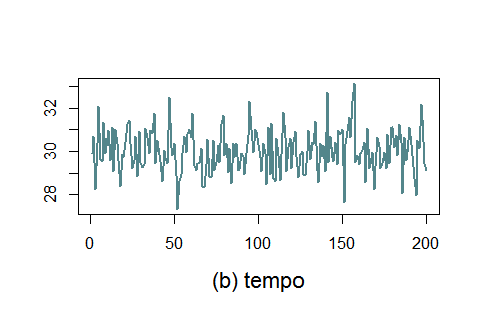
\includegraphics[width=0.48\linewidth]{03-SeriesTemp_files/figure-latex/stac-1} 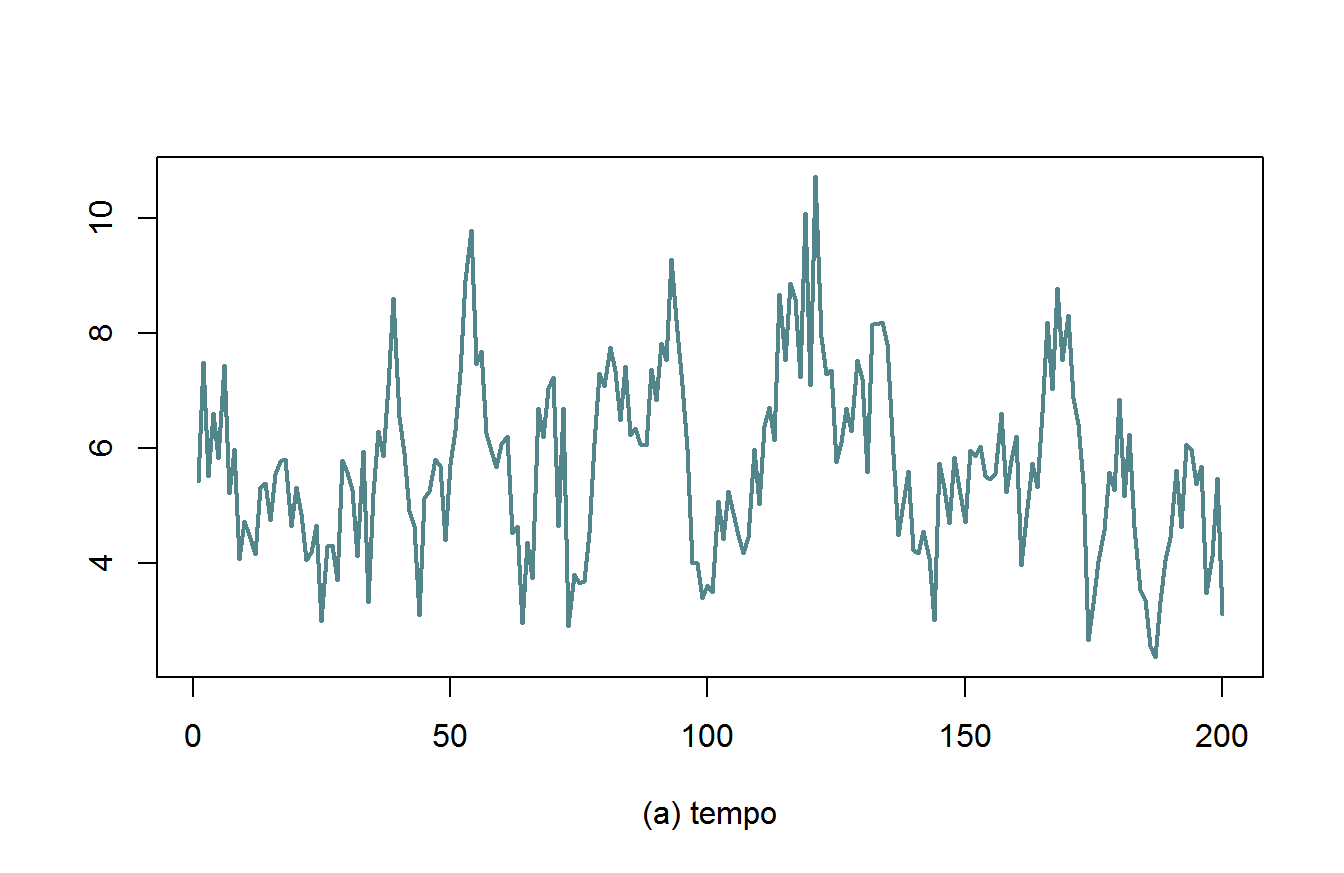
\includegraphics[width=0.48\linewidth]{03-SeriesTemp_files/figure-latex/stac-2} \caption{ Séries estacionárias: (a) Ruído branco, (b) ARMA(1,2).}\label{fig:stac}
\end{figure}

Entretanto, a maior parte das séries que encontramos na prática apresenta alguma forma de não-estacionariedade. A Figura \ref{fig:nstac} apresenta algumas séries que apresentam algum tipo de não-estacionariedade que podem resultar de diversas fontes. Algumas das fontes mais comuns de não-estacionariedade de uma série temporal são:

~~~a) a presença de uma tendência determinística (linear, logaritmica, exponencial, etc.) ao redor da qual a série se desenvolve. Geralmente a presença de uma tendência determinística é facilmente reconhecível através do gráfico. Na Figura \ref{fig:nstac}(a) apresentamos o gráfico de uma série apresentando uma tendência linear.

~~~b) quebra estrutural na série, que pode ser decorrente de uma mudança na média, como representado na Figura \ref{fig:nstac}(b), ou uma mudança mais sutil, difícil de ser detectada, como por exemplo mudanças na distribuição da série, na variância, no modelo da série, etc.

~~~c) presença do que chamamos de tendência estocástica, como representado na Figura \ref{fig:nstac}(c). Neste caso a série parece ``\emph{vagar}'' por um caminho que apresenta mudanças aleatórias de trajetória, sendo que fica difícil determinar o seu comportamento.

~~~d) presença de sazonalidade. Neste caso a sazonalidade provoca uma mudança de nível local fazendo com que a média da série se altere nos períodos sazonais. Um exemplo de série sazonal é dado na Figura \ref{fig:nstac}(d).

Mais detalhes serão apresentados adiante. A maior parte das séries que encontramos na prática apresenta alguma forma de não-estacionariedade. As séries econômicas apresentam em geral tendências lineares e muito comumente, tendência estocástica. Podemos ter, também, uma forma de não-estacionariedade explosiva, como o crescimento de uma colônia de bactérias.

\begin{figure}
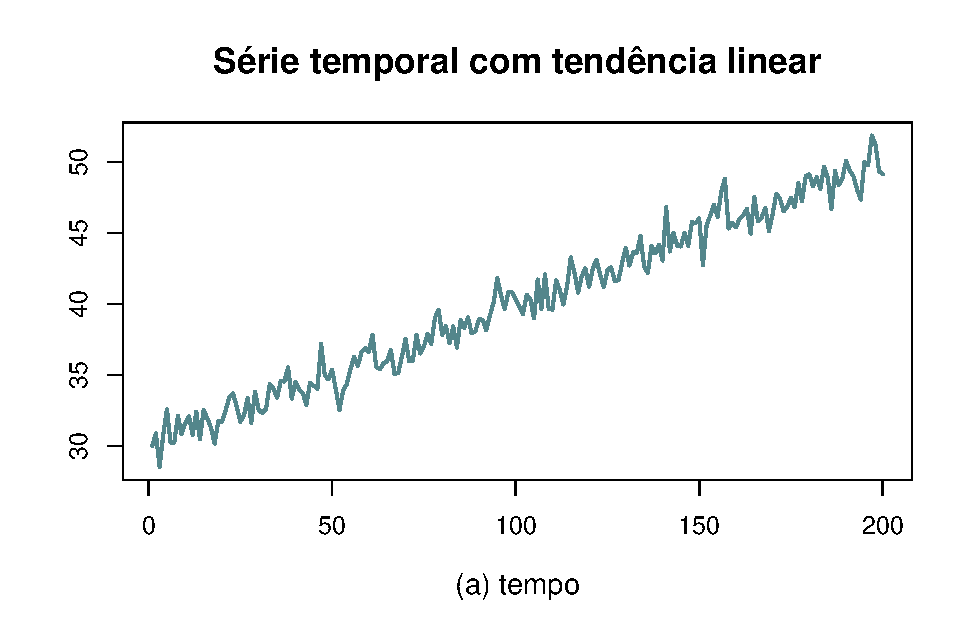
\includegraphics[width=0.48\linewidth]{03-SeriesTemp_files/figure-latex/nsstac-1} 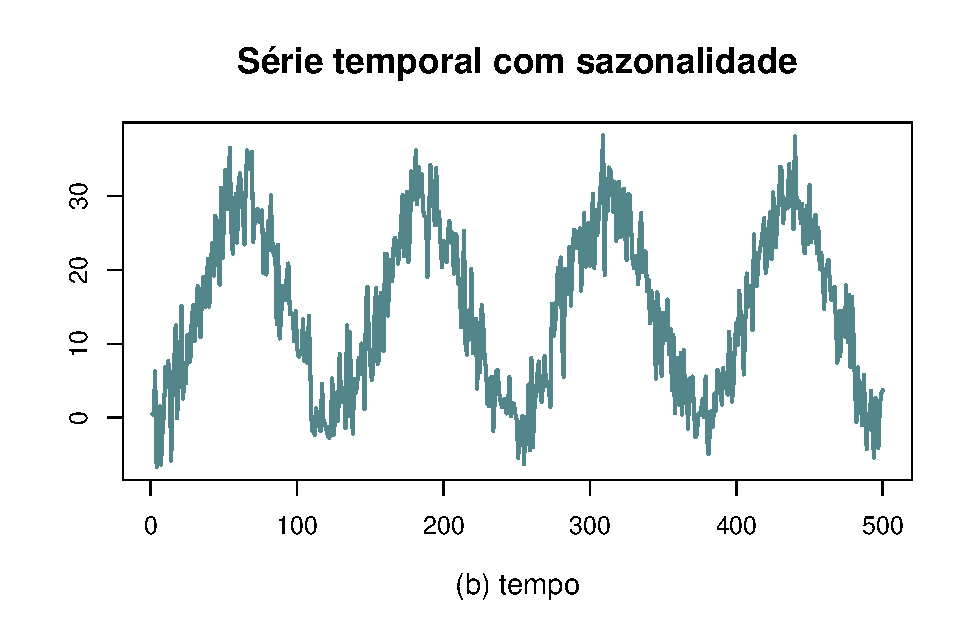
\includegraphics[width=0.48\linewidth]{03-SeriesTemp_files/figure-latex/nsstac-2} 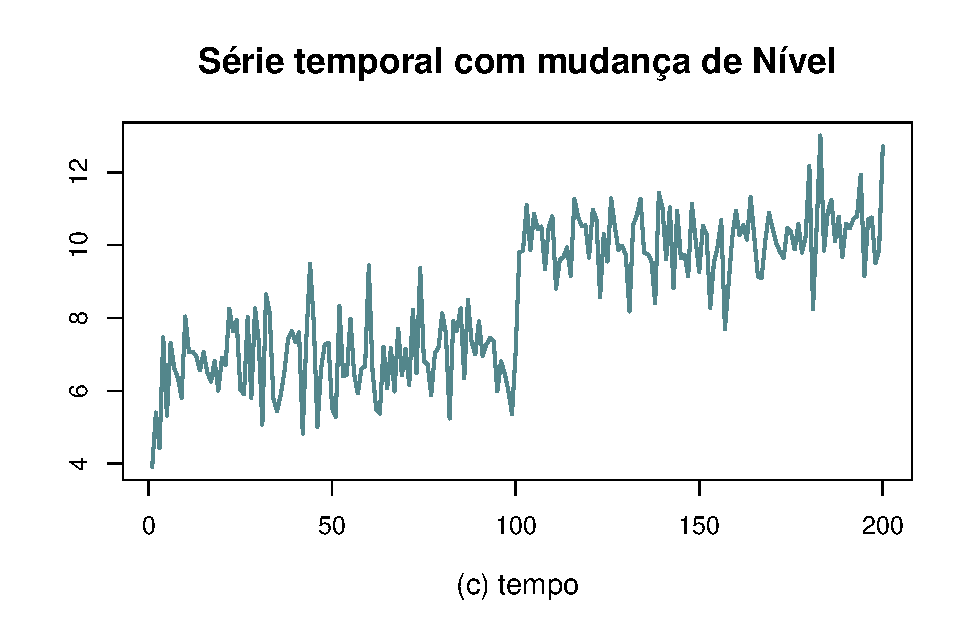
\includegraphics[width=0.48\linewidth]{03-SeriesTemp_files/figure-latex/nsstac-3} 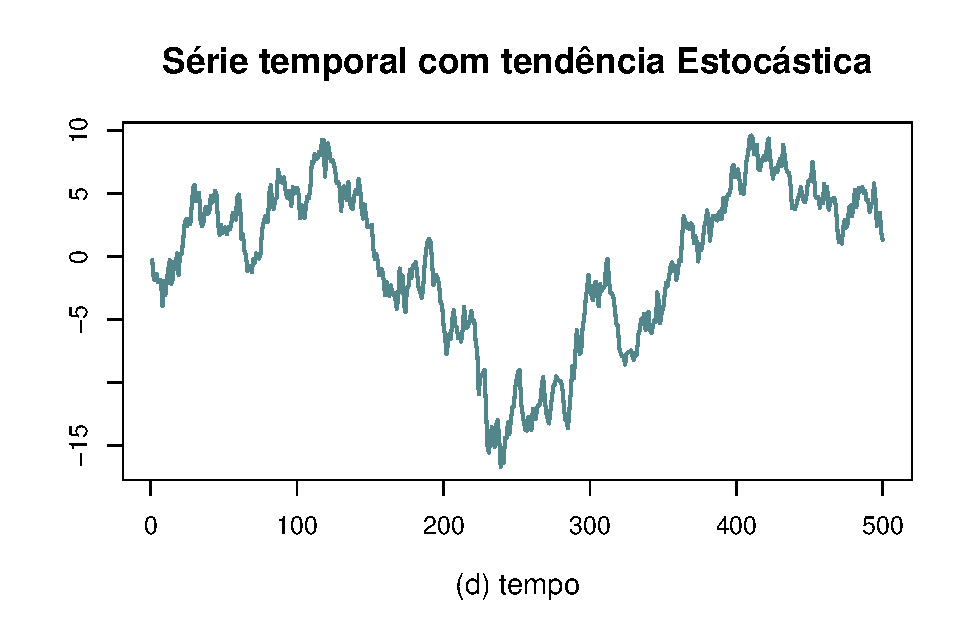
\includegraphics[width=0.48\linewidth]{03-SeriesTemp_files/figure-latex/nsstac-4} \caption{ Séries não-estacionárias apresentando: (a) Tendência linear, (b) quebra estrutural representada pela mudança de nível da série, (c) tendência estocástica e (d) sazonalidade.}\label{fig:nsstac}
\end{figure}

\hypertarget{estacionariedade-forte-ou-estrita}{%
\subsection{Estacionariedade forte ou estrita}\label{estacionariedade-forte-ou-estrita}}

Um processo estocástico \(Z(t)\) é dito ser um processo \textcolor{blue}{processo fortemente (ou estritamente) estacionário} se a distribuição conjunta de \(Z_{t_1},\cdots, Z_{t_n}\) é a mesma de \(Z_{t_1 - k}, Z_{t_2-k},\cdots, Z_{t_n - k}\), para todas as combinações de tempos \(t_1, \cdots, t_n\) e para todo \(k\in\mathbb{Z}\). Observe que este conceito se traduz em dizer que fixados os tempos \(t_1, \cdots, t_n\), ao andarmos \(k\) passos à frente homogeneamente no tempo, a distribuição das variáveis não se altera.

Quando \(n = 1\), a distribuição de \(Z_t\) é igual a distribuição de \(Z_{t-k}\) para qualquer \(k\), ou seja, os \(Z_t\)'s são identicamente distribuídos. Isto implica que num processo fortemente estacionário, as funções média (\(\mu_t\)) e variância (\(\sigma^2_t\)) são constantes para todo \(t\), isto é,
\(\sigma^2=\mbox{Var}(Z_t) = \mbox{Var}(Z_{t-k})\) e \(\mu=\mathbb{E} (Z_t ) = \mathbb{E} (Z_{t-k} )\), independentemente de \(t\) e \(k\). Quando \(n = 2\), a distribuição de \((Z_t, Z_s)\) é a mesma de \((Z_{t-k}, Z_{s-k} )\), de onde segue que \(\mbox{Cov}(Z_t, Z_s ) = \mbox{Cov}(Z_{t-k}, Z_{s-k} )\), para todo \(t,s\) e \(k\).

~~~Fazendo \(k = s\) temos:

\[\gamma(t,s)= \mbox{Cov}(Z_t, Z_s) = \mbox{Cov}(Z_{t-k}, Z_{s-k} )=\mbox{Cov}(Z_{t-s}, Z_{s-s} ) = \mbox{Cov}(Z_{t-s}, Z_0 )=\gamma(t-s,0);\]
e se \(k=t\),
\[ \gamma(t,s)= \mbox{Cov}(Z_{t-t}, Z_{s-t} ) = \mbox{Cov} (Z_0 , Z_{s-t} )= \mbox{Cov} (Z_0 , Z_{t-s} )= \gamma(0,s-t),\]

~~~de onde podemos concluir que

\begin{equation*}
\gamma(t,s) = \gamma(0,|t-s|),\quad \mbox{ lembrando que }\ \
|t - s| =\begin{cases}
t - s, & \mbox{ para  } t > s;\\
s - t, & \mbox{ para } s > t.
\end{cases}
\end{equation*}

Analogamente para a função de autocorrelação. Ou seja, num processo fortemente estacionário a covariância entre \(Z_t\) e \(Z_s\) depende somente da diferença temporal \(|t - s|\) e não dos tempos \(t\) e \(s\). Ou ainda, podemos dizer que a \(\mbox{Cov}(Z_t,Z_{t+h})\) depende apenas da distância temporal \(h\) entre as variáveis (chamada de \textbackslash textcolor\{blue\}\{\emph{defasagem}\} ou \textbackslash textcolor\{blue\}\{\emph{lag}\} entre as variáveis), e não do tempo \(t\). Isto permite simplificar a notação:

\[ \gamma(h)= \mbox{Cov}(Z_t, Z_{t-h} )=\mbox{Cov}(Z_t, Z_{t+h} )\]
\[ \rho(h)= \mbox{cor}(Z_t, Z_{t-h} )= \mbox{cor}(Z_t, Z_{t+h} ),\]

~para todo \(t,h\in\mathbb{Z}\). As propriedades gerais da \emph{FAC} e \emph{FACV} para um processo estacionário são:

~~~1) \(\gamma(0) = \mbox{Var}(Z_t)\), \quad \(\rho(0) = 1\);

~~~2) \(\gamma(h) = \gamma(-h)\),\quad \(\rho(h) = \rho(-h)\);

~~~3) \(|\gamma(h)|\leq \gamma(0)\), \quad \(|\rho(h)|\leq 1\).

Se um processo é estritamente estacionário e tem variância finita, então a \emph{FACV} depende somente do \emph{lag} \(h\).

\hypertarget{estacionariedade-fraca-ou-de-segunda-ordem}{%
\subsection{Estacionariedade fraca ou de segunda ordem}\label{estacionariedade-fraca-ou-de-segunda-ordem}}

A estacionariedade forte é um conceito na maioria das vezes difícil de ser identificado na prática, mas muito conveniente do ponto de vista matemático. Uma outra maneira de se definir a estacionariedade de uma série de forma que a teoria é matematicamente tratável e de fácil detecção em problemas práticos é a seguinte: um processo estocástico \(Z_t\) é dito ser \textbackslash textcolor\{blue\}\{\emph{fracamente estacionário ou estacionário de segunda-ordem}\} se:

\begin{center}\rule{0.5\linewidth}{0.5pt}\end{center}

\begin{quote}
~~~a) a função média é constante para todo tempo \(t\);\\
\hspace*{0.333em}\hspace*{0.333em}\hspace*{0.333em}b) \(\gamma(t,t-h) = \gamma(0,h)=\gamma(h)\) para todo tempo \(t\) e lag \(h\).
\end{quote}

\begin{center}\rule{0.5\linewidth}{0.5pt}\end{center}

A condição \(\gamma(t,t-h) = \gamma(h)\) para todo tempo \(t\) e lag \(h\) é equivalente a \(\rho(t,t-h) = \rho(h)\). Além disso, \(\mbox{Var}(Z_t)=\gamma(0)\) não depende de \(t\). Como veremos adiante, em processos fracamente estacionários as funções de autocovariância e autocorrelação desempenham papel central no seu estudo. Neste trabalho, sempre que nos referirmos a um processo estacionário, estaremos nos referindo à processos fracamente estacionários.

\hypertarget{teste-para-significuxe2ncia-das-autocorrelauxe7uxf5es}{%
\subsection{Teste para significância das autocorrelações}\label{teste-para-significuxe2ncia-das-autocorrelauxe7uxf5es}}

Mais adiante quando estudarmos modelagem ARIMA, precisaremos de ferramentas para decidir se uma dada série é não-correlacionada. Para testar a hipótese conjunta de que \(\rho(1)=\cdots=\rho(m)=0\) contra a hipótese de que algum \(\rho(k)\neq0\), pode-se usar a estatística \(Q_{BP}\) desenvolvida por \textcolor{blue}{Box e Pierce}, ou a estatística \(Q_{LB}\) desenvolvida por \textcolor{blue}{Ljung-Box}, definidas, respectivamente, por:

\begin{center}\rule{0.5\linewidth}{0.5pt}\end{center}

\begin{quote}
\textcolor{blue}{Box e Pierce}
\[
Q_{BP}(m)={n}\sum_{k=1}^{m}\hat{\rho}_k^2(\hat{\varepsilon})
\]
em que \(n\) é o tamanho da amostra (série) e \(m\) é o maior lag considerado na hipótese. A estatística \(Q_{BP}\) em grandes amostras tem distribuição qui-quadrado com \(m\) graus de liberdade.
\end{quote}

\begin{center}\rule{0.5\linewidth}{0.5pt}\end{center}

\begin{center}\rule{0.5\linewidth}{0.5pt}\end{center}

\begin{quote}
\textcolor{blue}{Ljung-Box}
\[
Q_{LB}(m)={n(n+2)}\sum_{k=1}^{m}\frac{\hat{\rho}_k^2(\hat{\varepsilon})}{n-k}
\]
a qual se distribui como uma qui-quadrado com \(m\) graus de liberdade em
grandes amostras. A estatística \(Q_{LB}\) possui maior poder para amostras
pequenas que a estatística \(Q_{BP}\).
\end{quote}

\begin{center}\rule{0.5\linewidth}{0.5pt}\end{center}

Observe que a hipótese nula do teste é que todas as correlações de lag \(1,\cdots,m\) são nulas, para algum \(m\) predeterminado, desta forma a escolha do valor de \(m\) é fundamental. Quanto maior o \(m\), caso não seja possível rejeitar a hipótese nula, menor é a evidencia de que a série testada é correlacionada. Porém, se \(m\) for muito grande, dois problemas poderão acontecer: primeiro, se \(m\) é muito próximo de \(n\) haverão poucos pontos amostrais com distância temporal \(m\) o que torna a estimação de \(\hat\rho_k(\hat\varepsilon)\) problemática, deteriorando a qualidade do teste; segundo, o poder do teste decresce com o aumento de \(m\). Embora não haja consenso na literatura sobre o valor ideal de \(m\), sugerimos utilizar \(m=20\) para séries com \(n\geq50\). Se a série for curta, na literatura encontra-se a sugestão \(m=\min(10,n/5)\).

\hypertarget{funuxe7uxe3o-de-autocorrelauxe7uxe3o-parcial-facp}{%
\subsection{\texorpdfstring{Função de autocorrelação parcial ( \emph{FACP} )}{Função de autocorrelação parcial ( FACP )}}\label{funuxe7uxe3o-de-autocorrelauxe7uxe3o-parcial-facp}}

A função de autocorrelação parcial ( \emph{FACP} ) entre as variáveis \(Y_t\) e \(Y_{t+k}\), denotada por \(\alpha(k)\) em processos estacionários, é a correlação entre as variáveis \(Y_t\) e \(Y_{t+k}\) removida a influência das variáveis intermediárias \(Y_{t+1},Y_{t+2},\cdots, Y_{t+k-1}\). Dada uma série temporal \(\{Y_t\}_{t=1}^\infty\) estacionária e uma variável aleatória \(X\), denotemos por \(\Pi_{r,s}(X)\) a projeção de \(X\) no subespaço gerado pelas variáveis \(Y_{r+1},\cdots,Y_{r+s-1}\). A FACP entre \(Y_t\) e \(Y_{t+k}\) é dada por
\[\alpha(k)=\mbox{Cor}\big(Y_t-\Pi_{t,k}(Y_t),Y_{t+k}-\Pi_{t,k}(Y_{t+k})\big), \mbox{ para }k\geq 2,\]
e \(\alpha(1)=\rho(1)\).

A \emph{FACP} para um processo estacionário com média zero pode ser obtida a partir da regressão
\begin{equation}
y_{t+k} = \phi_{k1} y_{t+k-1} + \phi_{k2} y_{t+k-2} +\cdots + \phi_{kk} y_{t}+\varepsilon_{t+k},
\end{equation}
da qual podem ser obtidas as equações de \emph{Yule-Walker}.

Multiplicando ambos os lados por \(y_{t+k-j}\) e calculando o valor dividindo pela variância, tem-se

\begin{equation*}
\rho_j = \phi_{k1}\rho_{j-1} + \phi_{k2}\rho_{j-2} +\cdots + \phi_{kk} \rho_{k-j}.
\end{equation*}
Então para \(j = 1, 2, \ldots, k\), temos:

\begin{eqnarray*}
\rho_1 &=& \phi_{k1}\rho_{0} + \phi_{k2}\rho_{1} +\cdots + \phi_{kk} \rho_{k-1};\\
\rho_2 &=& \phi_{k1}\rho_{1} + \phi_{k2}\rho_{0} +\cdots + \phi_{kk} \rho_{k-2};\\
&\vdots&\\
\rho_k &=& \phi_{k1}\rho_{k-1} + \phi_{k2}\rho_{k-2} +\cdots + \phi_{kk} \rho_{0};\\
\end{eqnarray*}

Para \(k = 1\) \(\rightarrow\) \(\hat{\phi}_{11} = \rho_1\).

Para \(k = 2\) \(\rightarrow\) \(\rho_1 = \phi_{21} + \phi_{22}\rho_1\) e \(\rho_2 = \phi_{21}\rho_1 + \phi_{22}\).

Ou podemos escrever a ultima equação em notação matricial:

\begin{equation*}
 \begin{bmatrix}
\rho_1 \\
\rho_2
\end{bmatrix}
=
 \begin{bmatrix}
1&\rho_1 \\
\rho_1&1
\end{bmatrix}
 \begin{bmatrix}
\phi_{21}\\
\phi_{22}
\end{bmatrix}.
\end{equation*}
cuja solução para o estimador de \(\phi_{22}\) é dada pela regra de \emph{Cramer}:

\begin{equation*}
\hat{\phi}_{22}=\frac{\begin{vmatrix}
1&\rho_1 \\
\rho_1&\rho_2
\end{vmatrix}}
{\begin{vmatrix}
1&\rho_1 \\
\rho_1&1
\end{vmatrix}}
\end{equation*}

Para \(k = 3\) temos as equações:
\begin{eqnarray*}
\rho_1 &=& \phi_{31}+ \phi_{32}\rho_1 + \phi_{33}\rho_2\\
\rho_2 &=& \phi_{31} \rho_1 + \phi_{32} + \phi_{33} \rho_1\\
\rho_3 &=& \phi_{31} + \phi_{32} \rho_1 + \phi_{33}.
\end{eqnarray*}

Em notação matricial temos:

\begin{equation*}
 \begin{bmatrix}
\rho_1 \\
\rho_2\\
\rho_3
\end{bmatrix}
=
 \begin{bmatrix}
1&\rho_1 &\rho_2\\
\rho_1&1 &\rho_1\\
\rho_2&\rho_1&1
\end{bmatrix}
 \begin{bmatrix}
\phi_{31}\\
\phi_{32}\\
\phi_{33}
\end{bmatrix}.
\end{equation*}
cuja solução para o estimador de \(\phi_{33}\) é dada por:

\begin{equation*}
\hat{\phi}_{33}=\frac{\begin{vmatrix}
1&\rho_1 &\rho_1\\
\rho_1&1 &\rho_2\\
\rho_2&\rho_1&\rho_3
\end{vmatrix}}
{\begin{vmatrix}
1&\rho_1 &\rho_2\\
\rho_1&1 &\rho_1\\
\rho_2&\rho_1&1
\end{vmatrix}},
\end{equation*}
e assim sucessivamente.

\hypertarget{operador-de-defasagem-ou-operador-lag}{%
\subsection{\texorpdfstring{Operador de defasagem ou operador \emph{lag}}{Operador de defasagem ou operador lag}}\label{operador-de-defasagem-ou-operador-lag}}

Em séries temporais é usual trabalhar com operadores que defasam a variável. Definimos então o operador de defasagem \(L\) como um operador linear tal que:

\begin{center}\rule{0.5\linewidth}{0.5pt}\end{center}

\begin{quote}
\textcolor{blue}{Operador defasagem}
\[
L^j y_t = y_{t-j}
\]
\end{quote}

\begin{center}\rule{0.5\linewidth}{0.5pt}\end{center}

As seguintes propriedades do operador \(L\) serão úteis no que segue:

~~~1) O operador lag aplicado a uma constante resulta na própria constante, isto é, \(Lc = c\);

~~~2) O operador lag segue a propriedade distributiva em relação à soma

\begin{equation*}
(L^i + L^j) Y_t = L^i Y_t + L^j Y_t = Y_{t-i} + Y_{t-j};
\end{equation*}

~~~3) É válida a propriedade associativa da multiplicação

\[L^i L^j Y_t = L^i (L^j Y_t ) = L^i (Y_{t-j} ) = Y_{t-i-j}.\]
Ou ainda \(L^i L^j Y_t = L^{i+j} Y_t = Y_{t-i-j}\);

~~~4) Potências negativas de \(L\) significam um operador de avanço,

\(L^{-i} Y_t =L^j Y_t\), fazendo \(j = -i\). Então \(L^{-i} Y_t = L^j Y_t = Y_{t-j} = Y_{t+i}\);

~~~5) Se \(|a| < 1\) definimos o operador inverso

\[(1-aL)^{-1} = 1 + aL + a^2 L^2 + \cdots = \sum_{j=0}^\infty (aL)^j.\]
A ação do operador \((1-aL)^{-1}\) em uma variável \(Y_t\) é a seguinte:
\[(1-aL)^{-1}(Y_t)=(1 + aL + a^2 L^2 + \cdots)(Y_t)=Y_t+aY_{t-1}+a^2Y_{t-2}+\cdots = \sum_{j=1}^\infty a^jY_{t-j}.\]
\noindent Note ainda que, para uma constante \(c\in\mathbb{R}\)
\[(1-aL)^{-1}(c)=(1 + aL + a^2 L^2 + \cdots)(c)=(c + aL(c) + a^2 L^2(c) + \cdots)=c\sum_{j=1}^\infty a^j=\frac{c}{1-a}\,.\]

~~~6) Se \(|a| > 1\), definimos o operador

\[ -aL( 1-aL)^{-1}=(1 + (aL)^{-1} + (aL)^{-2} +\cdots) \]
A ação do operador \(-aL(1-aL)^{-1}\) em uma variável \(Y_t\) é a seguinte:
\begin{align*}
(-aL(1-aL)^{-1})(Y_t)&=(1 + (aL)^{-1} + (aL)^{-2} +\cdots)(Y_t)= Y_t+\frac{1}{a}Y_{t+1}+\frac{1}{a^2}Y_{t+2}+\cdots\\
&=\sum_{j=1}^\infty \frac{1}{a^j}Y_{t+j}.
\end{align*}
Para uma constante \(c\in\mathbb{R}\), a ação do operador \(-aL(1-aL)^{-1}\) é dada por
\[(-aL(1-aL)^{-1})(c)=(1 + (aL)^{-1} + (aL)^{-2} +\cdots)(c)= c+\frac{c}{a}+\frac{c}{a^2}+\cdots=\frac{ca}{1-a}\,.\]

\hypertarget{ruuxeddo-branco}{%
\subsection{Ruído branco}\label{ruuxeddo-branco}}

Um importante exemplo de processo estacionário é o ruído branco, o qual é definido
como uma sequência de variáveis aleatórias \(\{\varepsilon_t \}_{t=-\infty}^{\infty}\) com as
seguintes propriedades:

\textcolor{blue}{Ruído Branco}

~~~1) \(\mathbb{E}(\varepsilon_t)=0\), para todo \(t\in\mathbb{R}\);

~~~2) \(\mathbb{E}(\varepsilon_t^2)=\sigma^2\) para todo \(t\in\mathbb{R}\);

~~~3) \(\mathbb{E}(\varepsilon_t\varepsilon_s)=0\), para todo \(t\neq s\), com \(t,s\in\mathbb{R}\).

Em outras palavras, um ruído branco é uma sequência de variáveis não-correlacionadas com média constante. \textcolor{blue}{ Denotaremos um processo ruído branco por RB($0,\sigma^2$)}. Escreveremos ainda \(\varepsilon_t\sim RB(0,\sigma_\varepsilon^2)\) para dizer que \(\{\varepsilon_t\}_{t}\) é um processo ruído branco com média 0 e variância \(\sigma^2_\varepsilon\)

Para um ruído branco \(\varepsilon_t\sim RB(0,\sigma_\varepsilon^2)\), \(\mu_t = \mathbb{E} (\varepsilon_t )=0\) é constante com \emph{FACV} e \emph{FAC} dadas por

\[
\gamma_\varepsilon(h) =\left\{
\begin{array}{cc}
\sigma^2_\varepsilon, & \mbox{ se  } h=0;\\
0, & \mbox{ se } h\neq0.
\end{array}\right.\qquad
\rho_\varepsilon(h) =\left\{\begin{array}{cc}
1, & \mbox{ se  } h=0;\\
0, & \mbox{ se } h \neq 0.
\end{array}\right.
\]

O termo ruído branco resulta do fato que em uma análise de frequência do modelo, podemos mostrar que todas as frequências são iguais. As características de um processo ruído branco ficam explícitas quando analisamos o seguinte gráfico

\begin{Shaded}
\begin{Highlighting}[]
\KeywordTok{set.seed}\NormalTok{(}\DecValTok{5647}\NormalTok{)}
\NormalTok{eps=}\KeywordTok{rnorm}\NormalTok{(}\DecValTok{200}\NormalTok{)}

\KeywordTok{plot}\NormalTok{(eps,}\DataTypeTok{type=}\StringTok{"l"}\NormalTok{,}\DataTypeTok{lwd=}\DecValTok{2}\NormalTok{,}\DataTypeTok{cex.lab=}\FloatTok{1.4}\NormalTok{, }\DataTypeTok{xlab=}\StringTok{"Ruído Branco"}\NormalTok{,}\DataTypeTok{ylab=}\StringTok{""}\NormalTok{, }\DataTypeTok{cex.main=}\FloatTok{1.7}\NormalTok{,}\DataTypeTok{col=}\StringTok{"cadetblue4"}\NormalTok{)}
\KeywordTok{acf}\NormalTok{(eps,}\DataTypeTok{lwd=}\DecValTok{2}\NormalTok{,}\DataTypeTok{cex.lab=}\FloatTok{1.4}\NormalTok{, }\DataTypeTok{xlab=}\StringTok{" lag "}\NormalTok{, }\DataTypeTok{main=}\StringTok{" "}\NormalTok{, }\DataTypeTok{cex.main=}\FloatTok{1.7}\NormalTok{,}\DataTypeTok{col=}\StringTok{"cadetblue4"}\NormalTok{)}
\KeywordTok{pacf}\NormalTok{(eps,}\DataTypeTok{lwd=}\DecValTok{2}\NormalTok{,}\DataTypeTok{cex.lab=}\FloatTok{1.4}\NormalTok{, }\DataTypeTok{xlab=}\StringTok{" lag "}\NormalTok{, }\DataTypeTok{main=}\StringTok{" "}\NormalTok{, }\DataTypeTok{cex.main=}\FloatTok{1.7}\NormalTok{,}\DataTypeTok{col=}\StringTok{"cadetblue4"}\NormalTok{,}\DataTypeTok{ylim=}\KeywordTok{c}\NormalTok{(}\OperatorTok{-}\FloatTok{0.9}\NormalTok{,}\FloatTok{0.9}\NormalTok{))}
\end{Highlighting}
\end{Shaded}

\begin{figure}
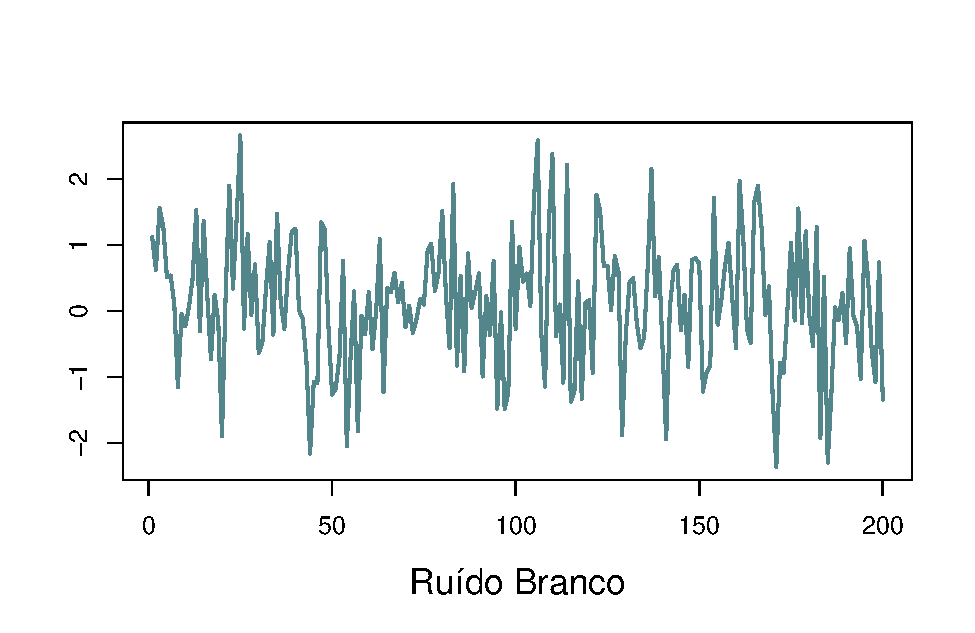
\includegraphics[width=0.33\linewidth]{03-SeriesTemp_files/figure-latex/rbsim-1} 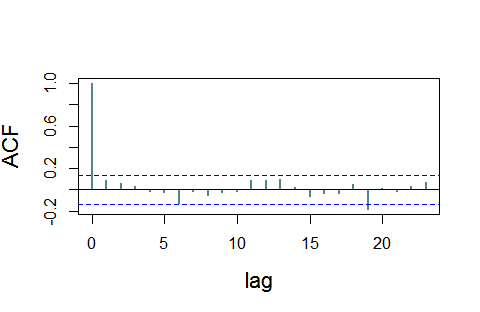
\includegraphics[width=0.33\linewidth]{03-SeriesTemp_files/figure-latex/rbsim-2} 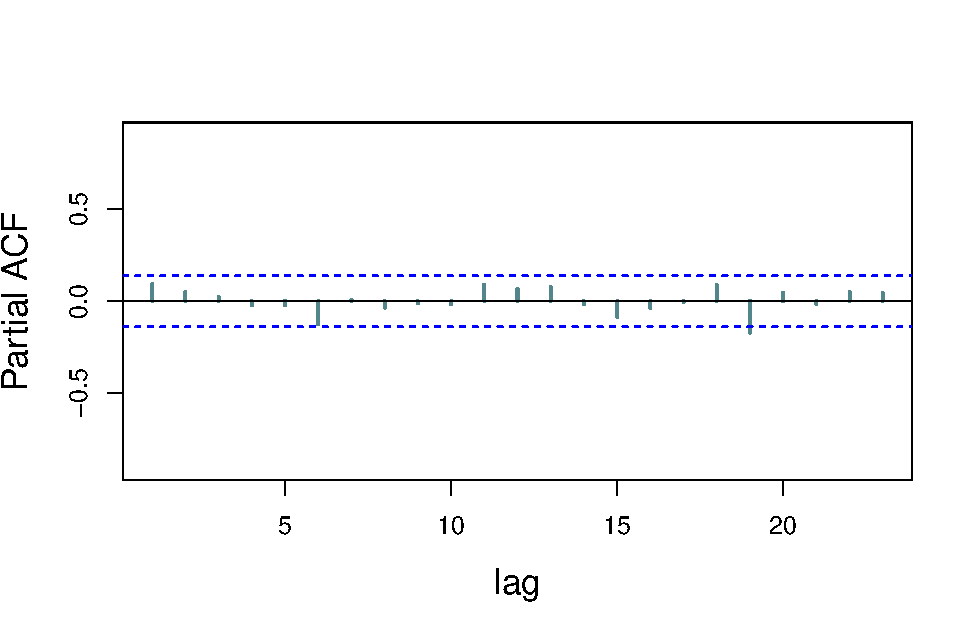
\includegraphics[width=0.33\linewidth]{03-SeriesTemp_files/figure-latex/rbsim-3} \caption{ Ruído branco gaussiano simulado,FAC amostral e FACP  amostral}\label{fig:rbsim}
\end{figure}

\begin{example}[Média-Móvel de ordem 1]
\protect\hypertarget{exm:unnamed-chunk-2}{}{\label{exm:unnamed-chunk-2} \iffalse (Média-Móvel de ordem 1) \fi{} }Este é um exemplo simples de um processo estacionário que não é um ruído branco. Suponha que
\end{example}
\textcolor{blue}{ Processo MA(1)}

\[
 Y_t = \varepsilon_t -0.5\varepsilon_{t-1},
\]
onde \(\varepsilon_t\) é um RB\((0,\sigma_\varepsilon^2)\).

\textcolor{blue}{ Média do MA(1)}

\[\mu_t= \mathbb{E} (Y_t ) = \mathbb{E} (\varepsilon_t ) - 0.5\mathbb{E} (\varepsilon_{t-1}) = 0\]

\textcolor{blue}{ Variância do MA(1)}

\[\mbox{Var}(Y_t ) = \mbox{Var} (\varepsilon_t - 0.5\varepsilon_{t-1} )= \sigma_\varepsilon^2 + 0.5\sigma_\varepsilon^2 = 1.25\sigma_\varepsilon^2.\]

Quanto à estrutura de covariância/correlação de um MA(1), temos
\begin{align}
\mbox{Cov}(Y_t,&Y_{t+h})=\mbox{Cov}(\varepsilon_t - 0.5\varepsilon_{t-1},\varepsilon_{t+h} - 0.5\varepsilon_{t+h-1})\nonumber\\
&=\mbox{Cov}(\varepsilon_t,\varepsilon_{t+h})-0.5\mbox{Cov}(\varepsilon_t,\varepsilon_{t+h-1})-0.5\mbox{Cov}(\varepsilon_{t-1},\varepsilon_{t+h})+0.25\mbox{Cov}(\varepsilon_{t-1},\varepsilon_{t+h-1})\nonumber\\
&= \gamma_\varepsilon(h)-0.5\gamma_\varepsilon(h-1)-0.5\gamma_\varepsilon(h+1)+0.25\gamma_\varepsilon(h),
\label{eq:gppo}
\end{align}
onde \(\gamma_\varepsilon\) denota a função de autocovariancia de \(\varepsilon_t\). Da equação \ref(eq:gppo), percebemos que \(\mbox{Cov}(Y_t,Y_{t+h})\) só é diferente de zero quando algum dos argumentos das funções à direita da igualdade em \ref(eq:gppo) é zero. Isto ocorre somente quando \(h=0\) (resultando em \(\mbox{Var}(Y_t)=1.25\sigma_\varepsilon^2\)) e quando \(|h|=1\) (resultando \(-0.5\sigma_\varepsilon^2\)). Em outras palavras, \(\mbox{Cov}(Y_t,Y_{t+h} )\) não depende de \(t\) e

\[\gamma(k) =\begin{cases} -0.5\sigma_\varepsilon^2, &\mbox{ se } |k|=1; \\
                                0,           & \mbox{ se } |k|>1.
               \end{cases}   \quad \mbox{e} \quad\rho(k) =\begin{cases} -0.4, &\mbox{ se } |k|=1; \\
                                0,           & \mbox{ se } |k|>1.
               \end{cases}   \]
Concluimos que um MA(1) é estacionário.

\hypertarget{metodologia-de-box-jenkins-ou-modelagem-arima}{%
\section{Metodologia de Box-Jenkins ou modelagem ARIMA}\label{metodologia-de-box-jenkins-ou-modelagem-arima}}

Na análise de séries temporais, a metodologia de Box-Jenkins, nomeada em homenagem ao estatísticos
George Box e Gwilym Meirion Jenkins, é uma metodologia pensada para a modelagem de séries temporais que é suficientemente simples de forma a atingir um grande público e suficientemente flexível para se aplicar a uma gama grande de problemas. Centrais à metodologia Box-Jenkins são os modelos \textbf{\emph{Autorregressivos Integrados de Média Móvel}}, abreviados modelos ARIMA, que representam uma classe grande de modelos capazes de modelar uma variedade de tipos de séries temporais. O intuito é modelar os valores da série temporal em função dos seus valores passados (admitindo um termo de erro) de forma que seja possível fazer previsões para esta série.
O procedimento pode ser resumido em três etapas:

\begin{itemize}
\item
  Identificação e seleção do modelo. Nesta etapa verificamos se as variáveis são estacionárias, identificando possíveis tendências e/ou sazonalidades na série, removendo-as quando detectadas. Fazemos o uso das funções de autocorrelação e autocorrelação parcial para decidir qual modelo da classe ARIMA é adequado para uma primeira tentativa de modelagem..
\item
  Estimação dos parâmetros usando algoritmos computacionais para chegar a coeficientes que melhor se adaptam ao modelo ARIMA selecionado. Os métodos mais comuns são a máxima verossimilhança e os mínimos quadráticos não-lineares.
\item
  Verificação do ajuste do modelo por meio de testes. Nesta fase, verificamos se o modelo estimado está em conformidade com as especificações do modelo teórico proposto. De suma importância é a análise residual na qual o objetivo é verificar se os resíduos satisfazem a hipótese de serem não-correlacionados. De grande utilidade é o teste Ljung-Box. Se o modelo proposto é inadequado, devemos voltar para a primeira etapa e propor um modelo alternativo.
\end{itemize}

Um dos modelos mais simples, útil e intuitivo é o modelo autorregressivo. Consideremos o caso mais simples.

\hypertarget{modelo-autorregressivo-de-ordem-1-ar1}{%
\subsection{Modelo autorregressivo de ordem 1 AR(1)}\label{modelo-autorregressivo-de-ordem-1-ar1}}

\textcolor{blue}{ Processo AR(1)}
\[
   Y_t = c + \phi Y_{t-1}+\varepsilon_t,
\]
em que \(\varepsilon_t\) é um \(RB(0,\sigma_\varepsilon^2)\).
\textbackslash end\{tcolorbox\}
Para calcularmos a média e a variância do processo, assumiremos primeiramente que os momentos incondicionais sejam iguais, de forma que \(\mathbb{E} Y_t=\mathbb{E} Y_{t-1}\). Com esta simplificação, fica fácil calcular a média de um processo AR(1):

\begin{center}\rule{0.5\linewidth}{0.5pt}\end{center}

\begin{quote}
\textcolor{blue}{ A média do processo AR(1)} é
\[
\mu= \mathbb{E} (Y_t)=\mathbb{E}(c) +\phi\mathbb{E} (Y_{t-1})+\mathbb{E}(\varepsilon_t)\quad\Longleftrightarrow\quad \mu=c+\phi\mu+0\quad\Longleftrightarrow\quad\mu=\frac{c}{1-\phi}\,,\]
desde que \(\phi\neq 1\). Se \(\phi=1\) a equação não possui solução \footnote{mais tarde veremos que para $\phi=1$ o processo é não estacionário e de fato  a média varia com $t$, sendo, portanto, falsa a hipótese inicial de que a média do processo é constante, utilizada para derivar as equações.}.
\end{quote}

\begin{center}\rule{0.5\linewidth}{0.5pt}\end{center}

Desta forma procedemos assumindo que \(\phi\neq 1\). Observe ainda que \(\mu=0\), quando \(c=0\). Para \(\phi\neq 1\), a variância de um AR(1), por sua vez, é dada por

\begin{center}\rule{0.5\linewidth}{0.5pt}\end{center}

\begin{quote}
\textcolor{blue}{ A variância do AR(1)} é
\[
\mbox{Var}(Y_t)=\mathbb{E}(Y_t^2)-\mu^2=\frac{\sigma^2}{1-\phi^2}.
\]
\end{quote}

\begin{center}\rule{0.5\linewidth}{0.5pt}\end{center}

Observe que se \(|\phi|>1\), a variância será negativa, o que é um absurdo. Neste caso as equações não são compatíveis com nenhum processo.
Quando \(|\phi|=1\), a variância de \(Y_t\) não está definida pois a média não está.

Deste exemplo, é possível concluir que é necessário estabelecer algumas restrições sobre o modelo para que se possa estimá-lo. Em particular,
uma condição necessária para estimar os coeficientes do modelo é que \(|\phi|<1\).

Com um pouco mais de trabalho, podemos encontrar o mesmo resultado sem a suposição de que os momentos incondicionais sejam iguais. Para isso usamos o operador defasagem \(L\) e suas propriedades para obtermos

\begin{align}
   Y_t = c + \phi Y_{t-1}+\varepsilon_t \quad &\Longleftrightarrow\quad (1-\phi L)Y_t=c+\varepsilon_t\quad \Longleftrightarrow\quad Y_t=(1-\phi L)^{-1}(c)+{(1-\phi L)}^{-1}(\varepsilon_t)\nonumber\\
\qquad &\Longleftrightarrow\qquad Y_t=\mu+\sum_{j=0}^{\infty}\phi^j\varepsilon_{t-j},
\label{eq:arcomomainfinito}
\end{align}
onde escrevemos \(\mu=c/(1-\phi)\) por simplicidade. A partir desta representação podemos facilmente obter

\begin{equation*}
\mathbb{E}  Y_t=\mu+\sum_{j=0}^{\infty}\phi^j\mathbb{E}(\varepsilon_{t-j})=\mu
\end{equation*}
e
\begin{align*}
\mbox{Var}(Y_t)&=\mathbb{E}(Y_t-\mu)^2=\mathbb{E}\bigg(\sum_{j=0}^{\infty}\phi^j\varepsilon_{t-j}\bigg)^2=\mathbb{E}\bigg(\sum_{j=0}^\infty\sum_{k=0}^\infty \phi^k\phi^j\varepsilon_{t-j}\varepsilon_{t-k}\bigg)\\
&=\sum_{j=0}^\infty\sum_{k=0}^\infty \phi^{k+j}\mathbb{E}(\varepsilon_{t-j}\varepsilon{t-k})=\sum_{j=0}^{\infty}\phi^{2j}\mathbb{E}(\varepsilon_{t-j}^2)=\frac{\sigma^2_\varepsilon}{1-\phi^2},
\end{align*}
onde a última igualdade segue do fato de que \(\mathbb{E}(\varepsilon_{t-j}\varepsilon_{t-k})=\gamma_\varepsilon(j-k)\) que é igual a zero se \(j\neq k\), e \(\sigma^2_\varepsilon\), se \(j=k\). Para \(h>0\), a

\begin{center}\rule{0.5\linewidth}{0.5pt}\end{center}

\begin{quote}
\textbackslash textcolor\{blue\}\{ função de autocovariância de \emph{lag}\} \(h\) é dada por
\begin{eqnarray*}
\gamma(h)&=&\mathbb{E}[(Y_t-\mu)(Y_{t-h}-\mu)]=\mathbb{E}\bigg[\bigg(\sum_{s=0}^{\infty}\phi^s\varepsilon_{t-s}\bigg)
\bigg(\sum_{k=0}^{\infty}\phi^k\varepsilon_{t-k-h}\bigg)\bigg]\\
&=&\sum_{s=0}^{\infty}\sum_{k=0}^{\infty}\phi^{k+s}\mathbb{E}(\varepsilon_{t-s}\varepsilon_{t-k-h})=\sum_{s=0}^{\infty}\sum_{k=0}^{\infty}\phi^{k+s}\gamma_\varepsilon(s-k-h).
\end{eqnarray*}
\end{quote}

\begin{center}\rule{0.5\linewidth}{0.5pt}\end{center}

Observe que \(\gamma_\varepsilon(s-k-h)\) só é diferente de zero quando \(s-k-h=0\), o que é equivalente a \(s=k+h\), assim
\begin{eqnarray*}
\gamma(h)=\sigma^2_\varepsilon\sum_{k=0}^{\infty}\phi^{2k+h}=\sigma^2_\varepsilon(\phi^h+\phi^{h+2}+\phi^{h+4}+\cdots)=\frac{\phi^h}{1-\phi^2}\sigma^2_\varepsilon,
\end{eqnarray*}
Para \(h<0\), analogamente obtemos
\[\gamma(h)=\frac{\phi^{-h}}{1-\phi^2}\sigma^2_\varepsilon,\]
ou seja, para \(h\neq0\),
\[\gamma(h)=\frac{\phi^{|h|}}{1-\phi^2}\sigma^2_\varepsilon.\]
Como a média e as covariâncias não são funções do tempo o processo é
fracamente estacionário, independente do valor de \(\phi\in(-1,1)\).

\begin{center}\rule{0.5\linewidth}{0.5pt}\end{center}

\begin{quote}
\textbackslash textcolor\{blue\}\{A função de autocorrelação de \emph{lag}\} \emph{h} é dada por
\begin{equation*}
\rho(h)= \frac{\frac{\phi^|h|}{1-\phi^2}\sigma^2}{\frac{\sigma^2}{1-\phi^2}}=\phi^{|h|}.
\end{equation*}
\end{quote}

\begin{center}\rule{0.5\linewidth}{0.5pt}\end{center}

Além disso, como \(|\phi|<1\), a função de autocorrelação é decrescente em \(|h|\).

\hypertarget{passeio-aleatuxf3rio-random-walk}{%
\subsection{\texorpdfstring{Passeio aleatório (\emph{Random Walk})}{Passeio aleatório (Random Walk)}}\label{passeio-aleatuxf3rio-random-walk}}

Quando \(\phi=1\) no caso anterior, temos o processo chamado passeio aleatório.
Seja \(\{\varepsilon_t\}_{t\in\mathbb{N}}\) um RB\((0, \sigma_\varepsilon^2)\).

\textcolor{blue}{ O Passeio aleatório } pode ser representado por
\[
Z_t = Z_{t-1} + \varepsilon_t,
\]
que pode ser reescrito de uma maneira bem simples. Defina inicialmente
\[Z_1=\varepsilon_1, \qquad Z_2=\varepsilon_1+\varepsilon_2 \leftrightarrow Z_2=Z_1+\varepsilon_2\]
e sucessivamente
\[Z_{k-1}=\varepsilon_1+\cdots+\varepsilon_{k-1}, \qquad Z_k=\varepsilon_1+\cdots+\varepsilon_{k-1}+\varepsilon_k = Z_{k-1}+\varepsilon_k. \]
Com esta representação, o cálculo da média e da variância de \(Z_t\) se tornam simples:

\textcolor{blue}{ A média do passeio aleatório } é
\[\mu_t= \mathbb{E}(Z_t) =\mathbb{E}(\varepsilon_1 + \varepsilon_2 +\cdots+ \varepsilon_t )= \mathbb{E} (\varepsilon_1 ) + \mathbb{E} (\varepsilon_2 ) +\cdots + \mathbb{E} (\varepsilon_t)= 0 + 0 + \cdots + 0 = 0,\]
e \textcolor{blue}{ a variância do passeio aleatório } é
\[\mbox{Var}(Z_t) = \mbox{Var}(\varepsilon_1 + \varepsilon_2 + \cdots + \varepsilon_t ) = \mbox{Var}(\varepsilon_1) + \cdots + \mbox{Var}(\varepsilon_t) = \sigma_\varepsilon^2 + \sigma_\varepsilon^2 + \cdots + \sigma_\varepsilon^2 = t\sigma_\varepsilon^2.\]
Assim concluímos que a variância de um passeio aleatório cresce linearmente com o tempo, sendo portanto um processo não-estacionário. Observe ainda que se \(1\leq t\leq s\), a função de autocovariância de um passeio aleatório é dada por
\begin{eqnarray*}
\gamma(t,s) &=&  \mbox{Cov}(Z_t,Z_s)\\
            &=&  \mbox{Cov}(\varepsilon_1 + \varepsilon_2 + \cdots + \varepsilon_t, \varepsilon_1 + \varepsilon_2 + \cdots + \varepsilon_s)\\
            &=& \sum_{i=1}^t\sum_{j=1}^s \mbox{Cov}(\varepsilon_i,\varepsilon_j)\\
            &=&  \mbox{Cov}(\varepsilon_1,\varepsilon_1) + \mbox{Cov}(\varepsilon_2,\varepsilon_2)+ \cdots+ \mbox{Cov}(\varepsilon_t,\varepsilon_t)\\
            &=&  \sigma_\varepsilon^2 + \sigma_\varepsilon^2 + \cdots +\sigma_\varepsilon^2 = t\sigma_\varepsilon^2
\end{eqnarray*}
onde \(\mbox{Cov}(\varepsilon_i, \varepsilon_j)=0\) para \(i\neq j\). O mesmo argumento mostra que se \(1\leq s \leq t\), teremos \(\gamma(t,s)=s\sigma_\varepsilon^2,\) de forma que podemos escrever compactamente \(\gamma(s,t)=\min(s,t)\sigma^2\).
A \textcolor{blue}{ função de autocorrelação de um passeio aleatório } é facilmente obtida
\begin{align*}
\rho(t,s)&= \frac{\gamma(s,t)}{\sqrt{\mbox{Var}(X_t)}\sqrt{\mbox{Var}(X_s)}}=\frac{\min(s,t)\sigma_\varepsilon^2}{\sqrt{t\sigma_\varepsilon^2}\sqrt{s\sigma_\varepsilon^2}}=\frac{\min(s,t)}{\sqrt{t}\sqrt{s}}=\left\{\begin{array}{cc}
           \frac{s}{\sqrt{t}\sqrt{s}}=\sqrt{\frac{s}{t}}, & \mbox{ se } 1\leq s\leq t; \\
           \frac{t}{\sqrt{t}\sqrt{s}}=\sqrt{\frac{t}{s}}, & \mbox{ se } 1\leq t\leq s
         \end{array}
\right.\\
&=\sqrt{\frac{\min(s,t)}{\max(s,t)}}.
\end{align*}

Em resumo, a \emph{FACV} e a \emph{FAC} de um passeio aleatório são dadas por

\begin{center}\rule{0.5\linewidth}{0.5pt}\end{center}

\begin{quote}
\textcolor{blue}{ FACV do passeio aleatório}
\[
\gamma(t,s) = \min(s,t)\sigma_\varepsilon^2,
\]
\end{quote}

\begin{center}\rule{0.5\linewidth}{0.5pt}\end{center}

\begin{center}\rule{0.5\linewidth}{0.5pt}\end{center}

\begin{quote}
\textcolor{blue}{ FAC do passeio aleatório}\\
\[
\rho(t,s)=\sqrt{\frac{\min(s,t)}{\max(s,t)}}
\]
\end{quote}

\begin{center}\rule{0.5\linewidth}{0.5pt}\end{center}

O passeio aleatório é um exemplo simples que serve de aproximação para diversas situações reais, tais como como o movimento comum de preços e títulos e também a posição de pequenas partículas suspensas dentro de um fluído, chamado movimento Browniano.

\begin{Shaded}
\begin{Highlighting}[]
\KeywordTok{set.seed}\NormalTok{(}\DecValTok{1231}\NormalTok{)}
\NormalTok{eps=}\KeywordTok{rnorm}\NormalTok{(}\DecValTok{200}\NormalTok{)}
\NormalTok{rw=}\KeywordTok{cumsum}\NormalTok{(eps)}
\KeywordTok{plot}\NormalTok{(rw,}\DataTypeTok{type=}\StringTok{"l"}\NormalTok{,}\DataTypeTok{lwd=}\DecValTok{2}\NormalTok{,}\DataTypeTok{cex.lab=}\FloatTok{1.4}\NormalTok{, }\DataTypeTok{xlab=}\StringTok{" tempo"}\NormalTok{,}\DataTypeTok{ylab=}\StringTok{""}\NormalTok{, }\DataTypeTok{main=}\StringTok{"(a)"}\NormalTok{, }\DataTypeTok{cex.main=}\FloatTok{1.7}\NormalTok{,}\DataTypeTok{col=}\StringTok{"cadetblue4"}\NormalTok{)}
\KeywordTok{acf}\NormalTok{(rw,}\DataTypeTok{type =} \StringTok{"correlation"}\NormalTok{,}\DataTypeTok{lag.max =} \DecValTok{50}\NormalTok{,}\DataTypeTok{cex.main=}\FloatTok{1.7}\NormalTok{,}\DataTypeTok{col=}\StringTok{"cadetblue4"}\NormalTok{,}\DataTypeTok{ylab=}\StringTok{"FAC"}\NormalTok{,}\DataTypeTok{lwd=}\DecValTok{4}\NormalTok{,}\DataTypeTok{main=}\StringTok{"(b)"}\NormalTok{)}
\KeywordTok{acf}\NormalTok{(rw,}\DataTypeTok{type =} \StringTok{"partial"}\NormalTok{ ,}\DataTypeTok{lag.max =} \DecValTok{50}\NormalTok{,}\DataTypeTok{cex.main=}\FloatTok{1.7}\NormalTok{,}\DataTypeTok{col=}\StringTok{"cadetblue4"}\NormalTok{,}\DataTypeTok{ylab=}\StringTok{"FACP"}\NormalTok{,}\DataTypeTok{lwd=}\DecValTok{4}\NormalTok{,}\DataTypeTok{main=}\StringTok{"(c)"}\NormalTok{)}
\end{Highlighting}
\end{Shaded}

\begin{figure}
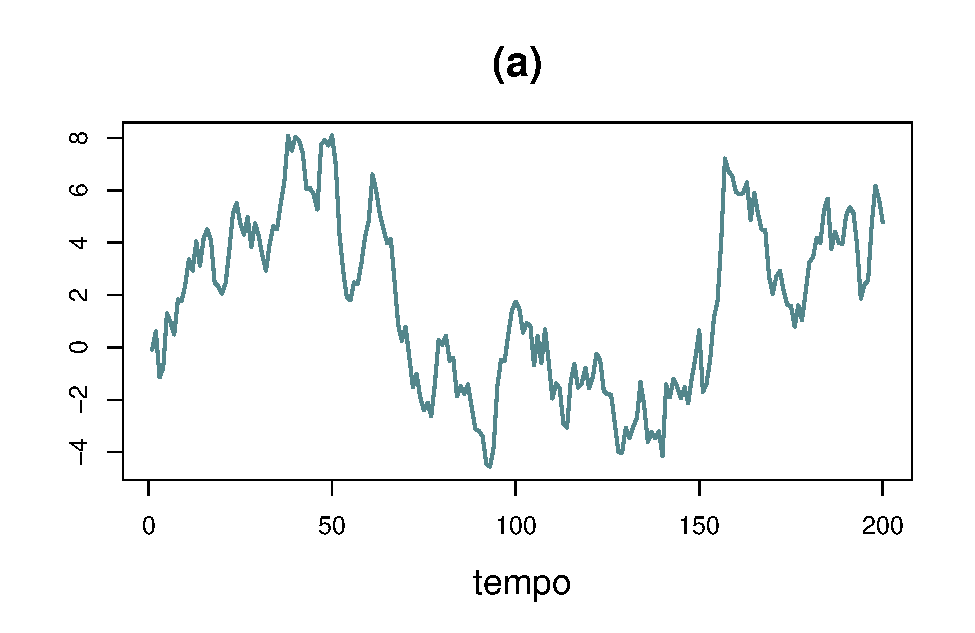
\includegraphics[width=0.3\linewidth]{03-SeriesTemp_files/figure-latex/rw-1} 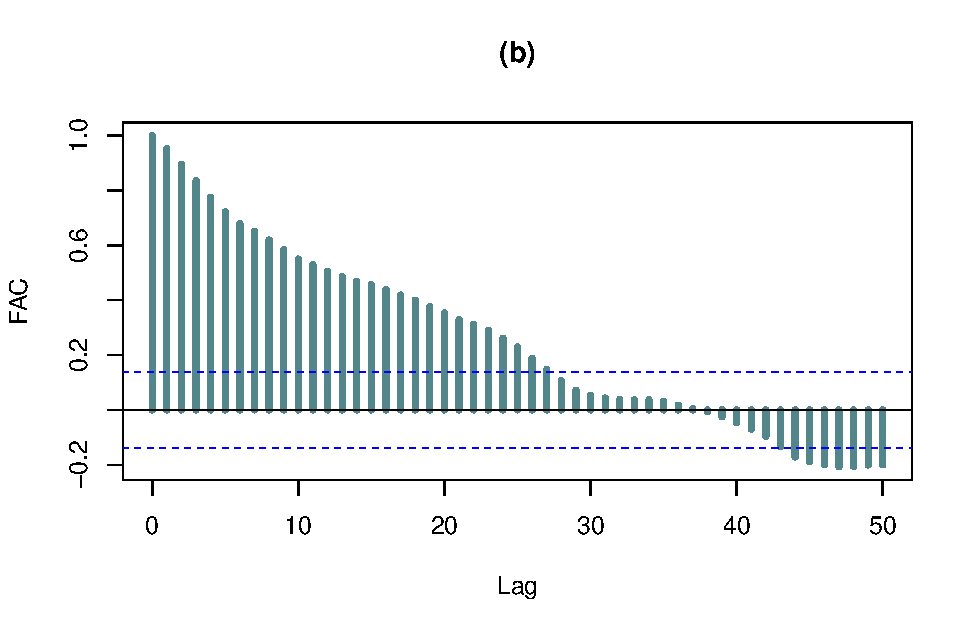
\includegraphics[width=0.3\linewidth]{03-SeriesTemp_files/figure-latex/rw-2} 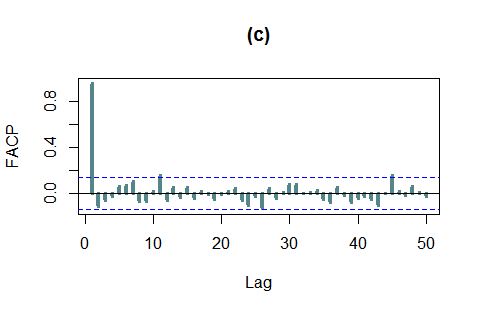
\includegraphics[width=0.3\linewidth]{03-SeriesTemp_files/figure-latex/rw-3} \caption{ Passeio aleatório simulado (a), FACV amostral (b) e FAC amostral (c).}\label{fig:rw}
\end{figure}

\hypertarget{modelos-autorregressivos-de-ordem-p-arp}{%
\subsection{\texorpdfstring{Modelos autorregressivos de ordem \(p\), AR(\(p\))}{Modelos autorregressivos de ordem p, AR(p)}}\label{modelos-autorregressivos-de-ordem-p-arp}}

O processo autorregressivo de ordem \(p\) é definido como

\begin{center}\rule{0.5\linewidth}{0.5pt}\end{center}

\begin{quote}
\textbackslash textcolor\{blue\}\{ O processo AR(\emph{p})\}\\
\[ Y_t=\phi_1Y_{t-1}+\cdots+\phi_pY_{t-p}+\varepsilon_t=\sum_{j=1}^{p}\phi_jY_{t-j} + \varepsilon_t.\]
\end{quote}

\begin{center}\rule{0.5\linewidth}{0.5pt}\end{center}

Escrevendo \(Y_t\) em função do operador \emph{lag}, obtemos

\begin{center}\rule{0.5\linewidth}{0.5pt}\end{center}

\begin{quote}
\textbackslash textcolor\{blue\}\{ Definição com o operador \emph{lag}\}\\
\begin{align*}
Y_t=\phi_1L(Y_t)+\phi_2L^2(Y_t)\cdots+\phi_pL^p(Y_t)+\varepsilon_t \quad &\Longleftrightarrow \quad (1-\phi_1L-\phi_2L^2-\cdots-\phi_pL^p)Y_t=\varepsilon_t \\
\quad &\Longleftrightarrow \quad  \Phi_p(L)Y_t=\varepsilon_t,
\end{align*}
\end{quote}

\begin{center}\rule{0.5\linewidth}{0.5pt}\end{center}

onde \(\Phi_p(L)=1-\phi_1L-\phi_2L^ 2-\cdots-\phi_pL^p\). O polinômio \(\Phi_p(\cdot)\) será importante no estudo da estacionariedade e causalidade de processos ARMA, que veremos adiante.

\hypertarget{alguns-processos-arma-simulados}{%
\subsubsection{Alguns processos ARMA simulados}\label{alguns-processos-arma-simulados}}

\begin{Shaded}
\begin{Highlighting}[]
\KeywordTok{set.seed}\NormalTok{(}\DecValTok{12322}\NormalTok{)}
\NormalTok{ar1=}\KeywordTok{arima.sim}\NormalTok{(}\DataTypeTok{n=}\DecValTok{200}\NormalTok{,}\DataTypeTok{model=}\KeywordTok{list}\NormalTok{(}\DataTypeTok{ar=}\FloatTok{0.5}\NormalTok{))}
\KeywordTok{plot}\NormalTok{(ar1,}\DataTypeTok{type=}\StringTok{"l"}\NormalTok{,}\DataTypeTok{lwd=}\DecValTok{2}\NormalTok{,}\DataTypeTok{cex.lab=}\FloatTok{1.4}\NormalTok{, }\DataTypeTok{xlab=}\StringTok{" tempo"}\NormalTok{,}\DataTypeTok{ylab=}\StringTok{""}\NormalTok{, }\DataTypeTok{main=}\StringTok{"(a)"}\NormalTok{, }\DataTypeTok{cex.main=}\FloatTok{1.7}\NormalTok{,}\DataTypeTok{col=}\StringTok{"cadetblue4"}\NormalTok{)}
\KeywordTok{acf}\NormalTok{(ar1,}\DataTypeTok{type =} \StringTok{"correlation"}\NormalTok{,}\DataTypeTok{lag.max =} \DecValTok{50}\NormalTok{,}\DataTypeTok{cex.main=}\FloatTok{1.7}\NormalTok{,}\DataTypeTok{col=}\StringTok{"cadetblue4"}\NormalTok{,}\DataTypeTok{ylab=}\StringTok{"FAC"}\NormalTok{,}\DataTypeTok{lwd=}\DecValTok{4}\NormalTok{,}\DataTypeTok{main=}\StringTok{"(b)"}\NormalTok{)}
\KeywordTok{acf}\NormalTok{(ar1,}\DataTypeTok{type =} \StringTok{"partial"}\NormalTok{ ,}\DataTypeTok{lag.max =} \DecValTok{50}\NormalTok{,}\DataTypeTok{cex.main=}\FloatTok{1.7}\NormalTok{,}\DataTypeTok{col=}\StringTok{"cadetblue4"}\NormalTok{,}\DataTypeTok{ylab=}\StringTok{"FACP"}\NormalTok{,}\DataTypeTok{lwd=}\DecValTok{4}\NormalTok{,}\DataTypeTok{main=}\StringTok{"(c)"}\NormalTok{)}
\end{Highlighting}
\end{Shaded}

\begin{figure}
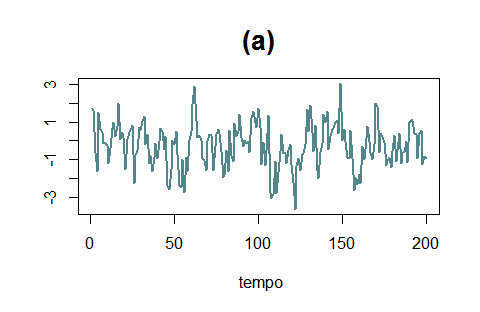
\includegraphics[width=0.33\linewidth]{03-SeriesTemp_files/figure-latex/ar105-1} 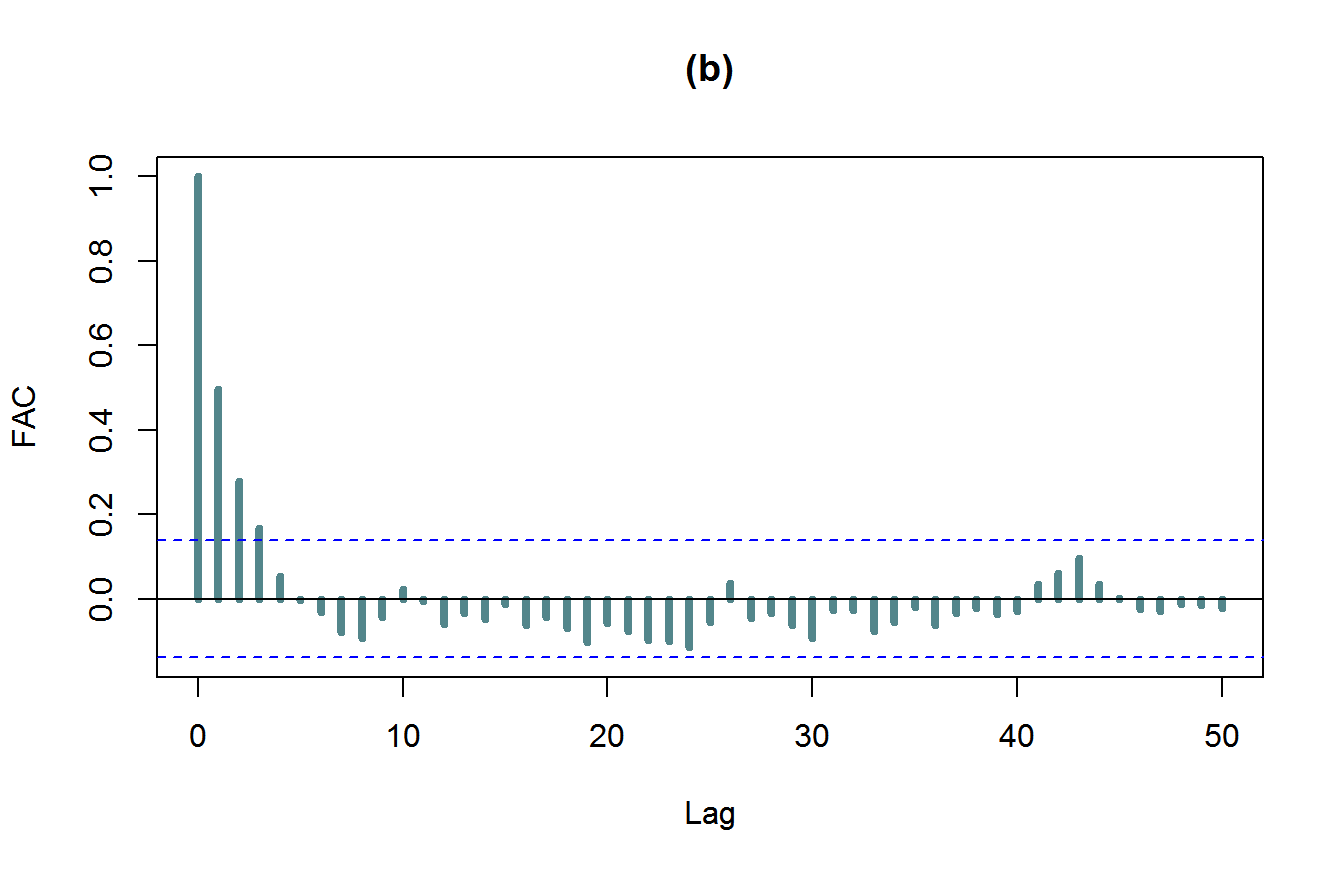
\includegraphics[width=0.33\linewidth]{03-SeriesTemp_files/figure-latex/ar105-2} 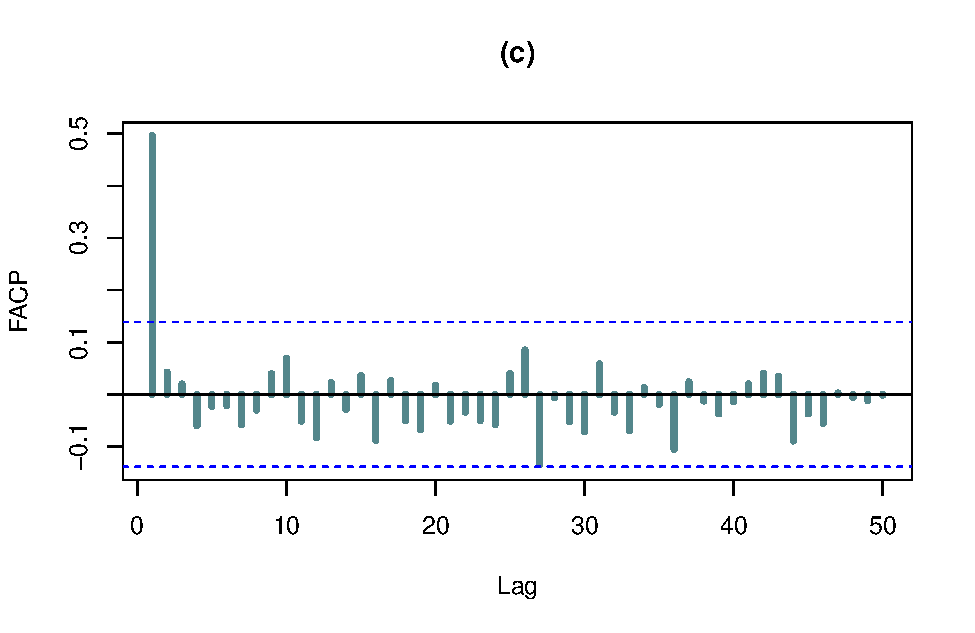
\includegraphics[width=0.33\linewidth]{03-SeriesTemp_files/figure-latex/ar105-3} \caption{AR(1) simulado com coeficiente $\phi_1=0.5$ (a), FACV amostral (b) e FAC amostral (c).}\label{fig:ar105}
\end{figure}

\begin{Shaded}
\begin{Highlighting}[]
\KeywordTok{set.seed}\NormalTok{(}\DecValTok{12322}\NormalTok{)}
\NormalTok{ar1m=}\KeywordTok{arima.sim}\NormalTok{(}\DataTypeTok{n=}\DecValTok{200}\NormalTok{,}\DataTypeTok{model=}\KeywordTok{list}\NormalTok{(}\DataTypeTok{ar=}\OperatorTok{-}\FloatTok{0.5}\NormalTok{))}
\KeywordTok{plot}\NormalTok{(ar1m,}\DataTypeTok{type=}\StringTok{"l"}\NormalTok{,}\DataTypeTok{lwd=}\DecValTok{2}\NormalTok{,}\DataTypeTok{cex.lab=}\FloatTok{1.4}\NormalTok{, }\DataTypeTok{xlab=}\StringTok{" tempo"}\NormalTok{,}\DataTypeTok{ylab=}\StringTok{""}\NormalTok{, }\DataTypeTok{main=}\StringTok{"(a)"}\NormalTok{, }\DataTypeTok{cex.main=}\FloatTok{1.7}\NormalTok{,}\DataTypeTok{col=}\StringTok{"cadetblue4"}\NormalTok{)}
\KeywordTok{acf}\NormalTok{(ar1m,}\DataTypeTok{type =} \StringTok{"correlation"}\NormalTok{,}\DataTypeTok{lag.max =} \DecValTok{50}\NormalTok{,}\DataTypeTok{cex.main=}\FloatTok{1.7}\NormalTok{,}\DataTypeTok{col=}\StringTok{"cadetblue4"}\NormalTok{,}\DataTypeTok{ylab=}\StringTok{"FAC"}\NormalTok{,}\DataTypeTok{lwd=}\DecValTok{4}\NormalTok{,}\DataTypeTok{main=}\StringTok{"(b)"}\NormalTok{)}
\KeywordTok{acf}\NormalTok{(ar1m,}\DataTypeTok{type =} \StringTok{"partial"}\NormalTok{ ,}\DataTypeTok{lag.max =} \DecValTok{50}\NormalTok{,}\DataTypeTok{cex.main=}\FloatTok{1.7}\NormalTok{,}\DataTypeTok{col=}\StringTok{"cadetblue4"}\NormalTok{,}\DataTypeTok{ylab=}\StringTok{"FACP"}\NormalTok{,}\DataTypeTok{lwd=}\DecValTok{4}\NormalTok{,}\DataTypeTok{main=}\StringTok{"(c)"}\NormalTok{)}
\end{Highlighting}
\end{Shaded}

\begin{figure}
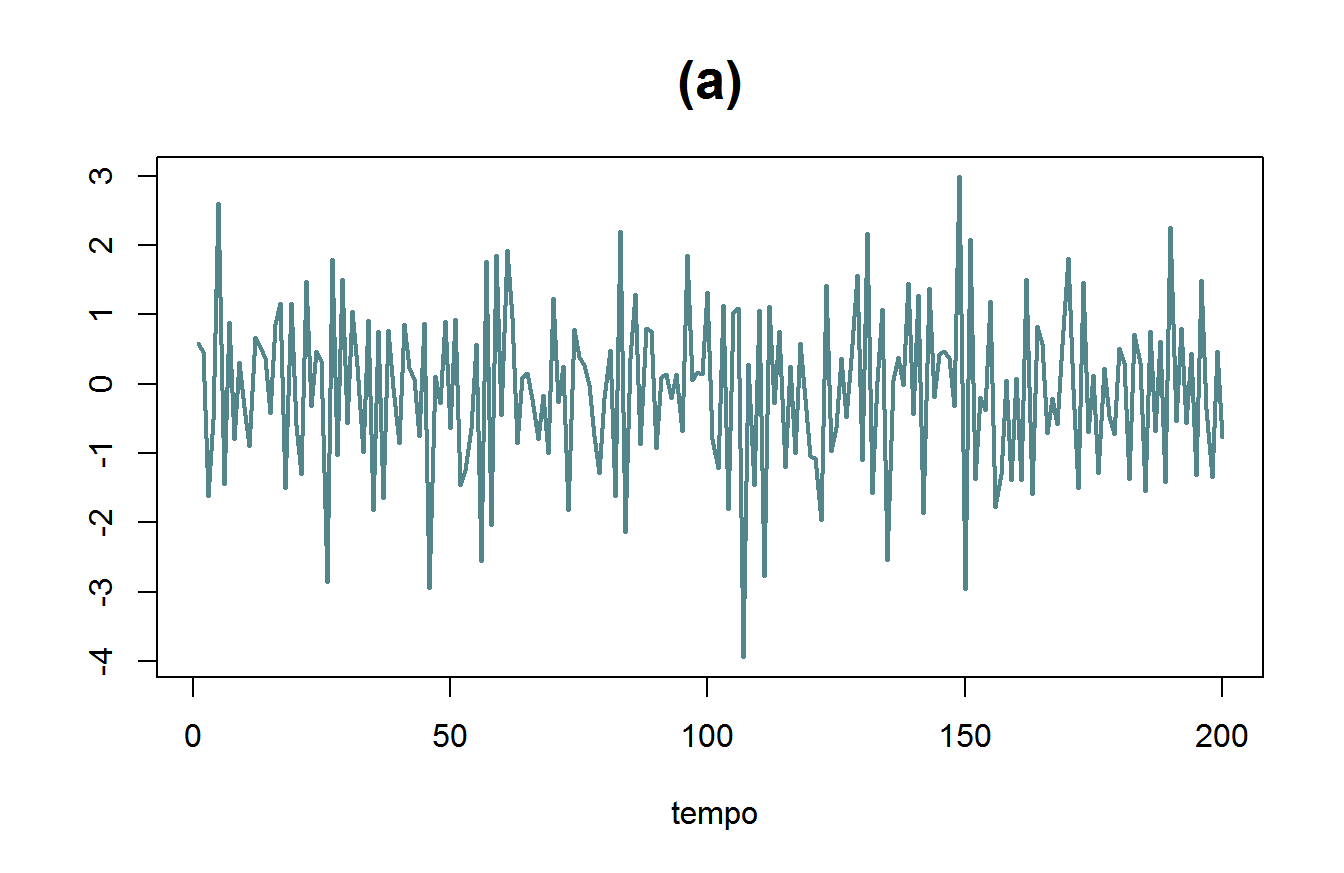
\includegraphics[width=0.33\linewidth]{03-SeriesTemp_files/figure-latex/arm105-1} 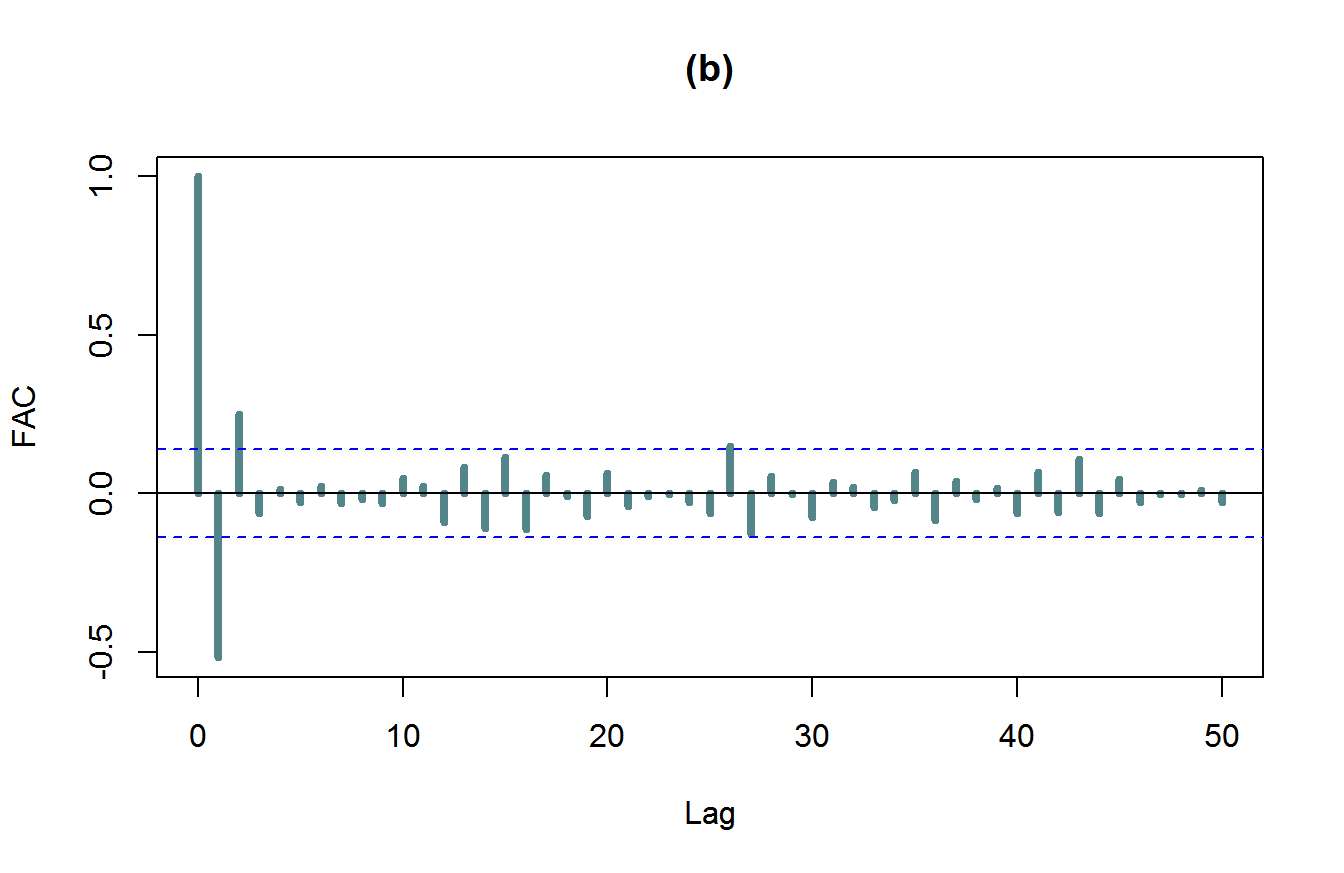
\includegraphics[width=0.33\linewidth]{03-SeriesTemp_files/figure-latex/arm105-2} 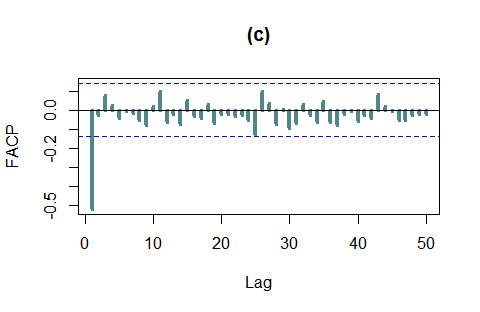
\includegraphics[width=0.33\linewidth]{03-SeriesTemp_files/figure-latex/arm105-3} \caption{AR(1) simulado com coeficiente $\phi_1=-0.5$ (a), FACV amostral (b) e FAC amostral (c).}\label{fig:arm105}
\end{figure}

\begin{Shaded}
\begin{Highlighting}[]
\KeywordTok{set.seed}\NormalTok{(}\DecValTok{12322}\NormalTok{)}
\NormalTok{ar108=}\KeywordTok{arima.sim}\NormalTok{(}\DataTypeTok{n=}\DecValTok{200}\NormalTok{,}\DataTypeTok{model=}\KeywordTok{list}\NormalTok{(}\DataTypeTok{ar=}\OperatorTok{-}\FloatTok{0.5}\NormalTok{))}
\KeywordTok{plot}\NormalTok{(ar108,}\DataTypeTok{type=}\StringTok{"l"}\NormalTok{,}\DataTypeTok{lwd=}\DecValTok{2}\NormalTok{,}\DataTypeTok{cex.lab=}\FloatTok{1.4}\NormalTok{, }\DataTypeTok{xlab=}\StringTok{" tempo"}\NormalTok{,}\DataTypeTok{ylab=}\StringTok{""}\NormalTok{, }\DataTypeTok{main=}\StringTok{"(a)"}\NormalTok{, }\DataTypeTok{cex.main=}\FloatTok{1.7}\NormalTok{,}\DataTypeTok{col=}\StringTok{"cadetblue4"}\NormalTok{)}
\KeywordTok{acf}\NormalTok{(ar108,}\DataTypeTok{type =} \StringTok{"correlation"}\NormalTok{,}\DataTypeTok{lag.max =} \DecValTok{50}\NormalTok{,}\DataTypeTok{cex.main=}\FloatTok{1.7}\NormalTok{,}\DataTypeTok{col=}\StringTok{"cadetblue4"}\NormalTok{,}\DataTypeTok{ylab=}\StringTok{"FAC"}\NormalTok{,}\DataTypeTok{lwd=}\DecValTok{4}\NormalTok{,}\DataTypeTok{main=}\StringTok{"(b)"}\NormalTok{)}
\KeywordTok{acf}\NormalTok{(ar108,}\DataTypeTok{type =} \StringTok{"partial"}\NormalTok{ ,}\DataTypeTok{lag.max =} \DecValTok{50}\NormalTok{,}\DataTypeTok{cex.main=}\FloatTok{1.7}\NormalTok{,}\DataTypeTok{col=}\StringTok{"cadetblue4"}\NormalTok{,}\DataTypeTok{ylab=}\StringTok{"FACP"}\NormalTok{,}\DataTypeTok{lwd=}\DecValTok{4}\NormalTok{,}\DataTypeTok{main=}\StringTok{"(c)"}\NormalTok{)}
\end{Highlighting}
\end{Shaded}

\begin{figure}
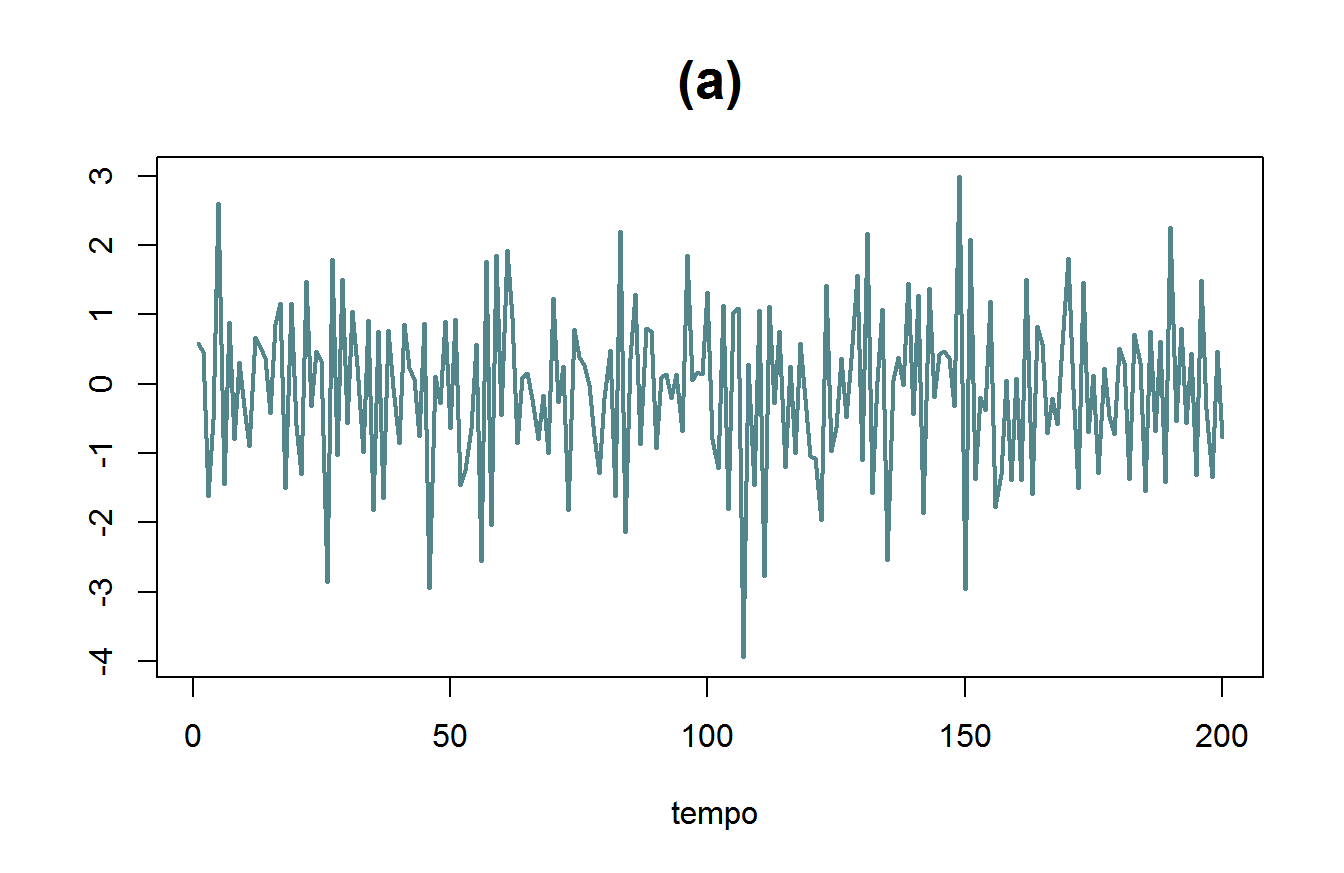
\includegraphics[width=0.33\linewidth]{03-SeriesTemp_files/figure-latex/ar108-1} 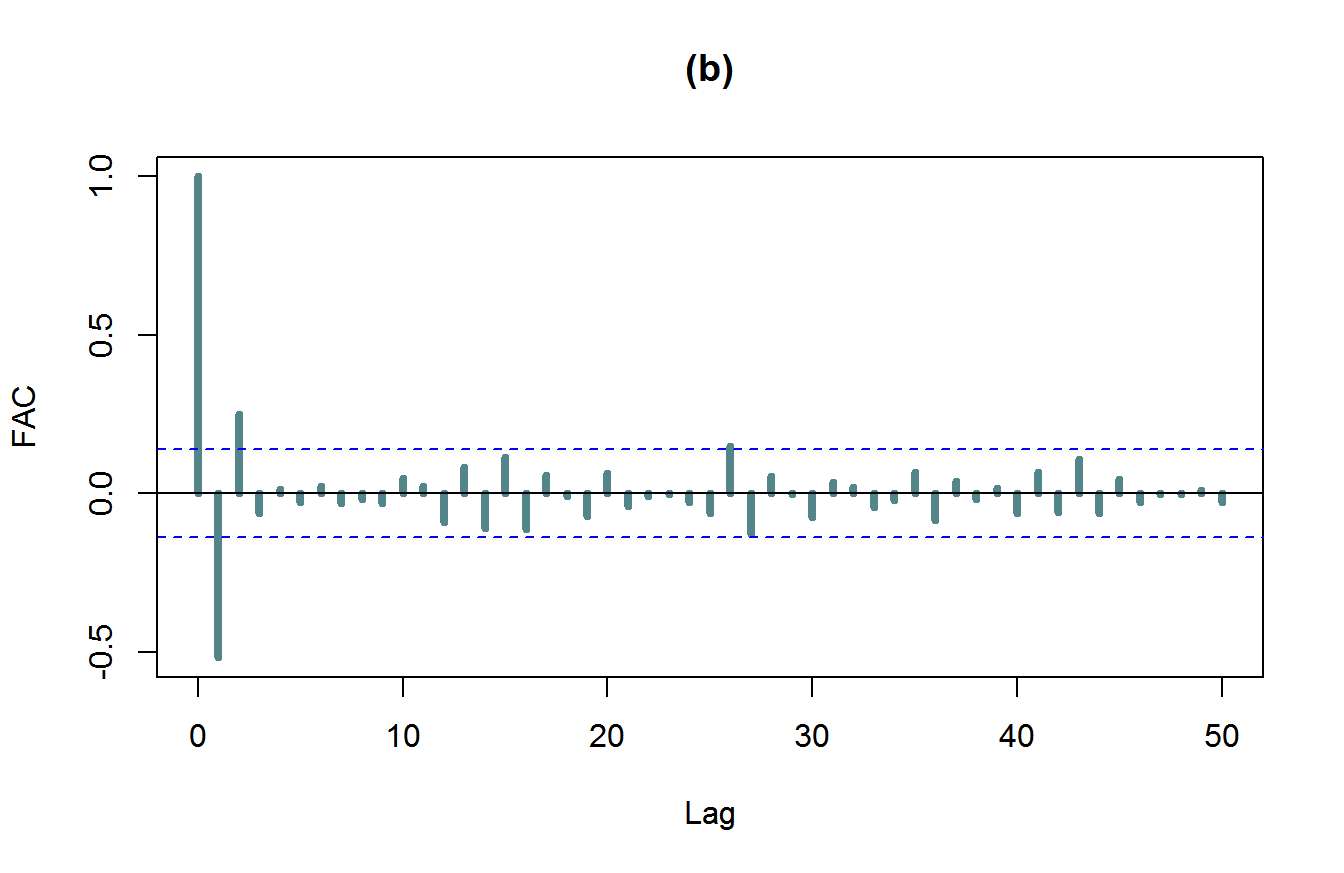
\includegraphics[width=0.33\linewidth]{03-SeriesTemp_files/figure-latex/ar108-2} 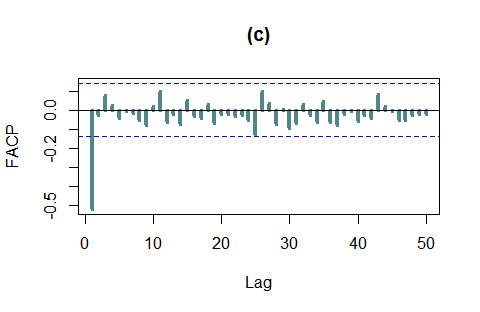
\includegraphics[width=0.33\linewidth]{03-SeriesTemp_files/figure-latex/ar108-3} \caption{AR(1) simulado com coeficiente $\phi_1=0.8$ (a), FACV amostral (b) e FAC amostral (c).}\label{fig:ar108}
\end{figure}

\begin{Shaded}
\begin{Highlighting}[]
\KeywordTok{set.seed}\NormalTok{(}\DecValTok{12322}\NormalTok{)}
\NormalTok{ar2=}\KeywordTok{arima.sim}\NormalTok{(}\DataTypeTok{n=}\DecValTok{200}\NormalTok{,}\DataTypeTok{model=}\KeywordTok{list}\NormalTok{(}\DataTypeTok{ar=}\KeywordTok{c}\NormalTok{(}\FloatTok{0.5}\NormalTok{,}\OperatorTok{-}\FloatTok{0.7}\NormalTok{)))}
\KeywordTok{plot}\NormalTok{(ar2,}\DataTypeTok{type=}\StringTok{"l"}\NormalTok{,}\DataTypeTok{lwd=}\DecValTok{2}\NormalTok{,}\DataTypeTok{cex.lab=}\FloatTok{1.4}\NormalTok{, }\DataTypeTok{xlab=}\StringTok{" tempo"}\NormalTok{,}\DataTypeTok{ylab=}\StringTok{""}\NormalTok{, }\DataTypeTok{main=}\StringTok{"(a)"}\NormalTok{, }\DataTypeTok{cex.main=}\FloatTok{1.7}\NormalTok{,}\DataTypeTok{col=}\StringTok{"cadetblue4"}\NormalTok{)}
\KeywordTok{acf}\NormalTok{(ar2,}\DataTypeTok{type =} \StringTok{"correlation"}\NormalTok{,}\DataTypeTok{lag.max =} \DecValTok{50}\NormalTok{,}\DataTypeTok{cex.main=}\FloatTok{1.7}\NormalTok{,}\DataTypeTok{col=}\StringTok{"cadetblue4"}\NormalTok{,}\DataTypeTok{ylab=}\StringTok{"FAC"}\NormalTok{,}\DataTypeTok{lwd=}\DecValTok{4}\NormalTok{,}\DataTypeTok{main=}\StringTok{"(b)"}\NormalTok{)}
\KeywordTok{acf}\NormalTok{(ar2,}\DataTypeTok{type =} \StringTok{"partial"}\NormalTok{ ,}\DataTypeTok{lag.max =} \DecValTok{50}\NormalTok{,}\DataTypeTok{cex.main=}\FloatTok{1.7}\NormalTok{,}\DataTypeTok{col=}\StringTok{"cadetblue4"}\NormalTok{,}\DataTypeTok{ylab=}\StringTok{"FACP"}\NormalTok{,}\DataTypeTok{lwd=}\DecValTok{4}\NormalTok{,}\DataTypeTok{main=}\StringTok{"(c)"}\NormalTok{)}
\end{Highlighting}
\end{Shaded}

\begin{figure}
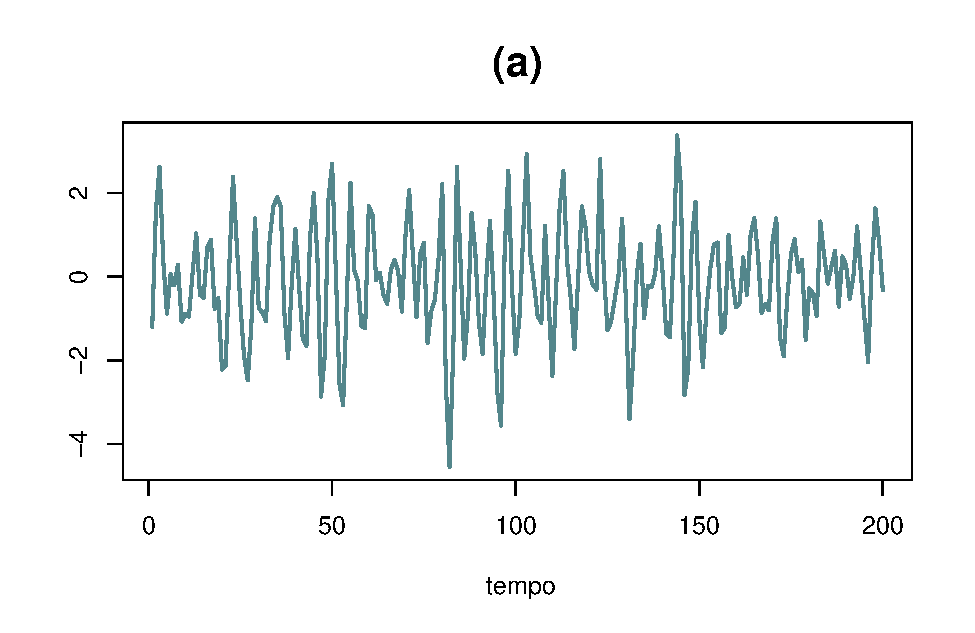
\includegraphics[width=0.33\linewidth]{03-SeriesTemp_files/figure-latex/ar2-1} 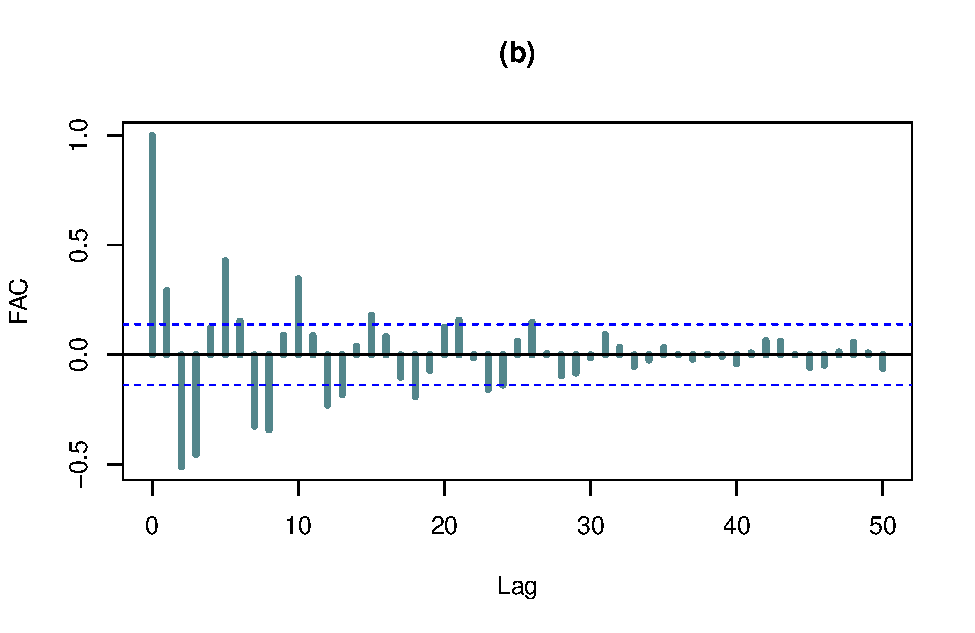
\includegraphics[width=0.33\linewidth]{03-SeriesTemp_files/figure-latex/ar2-2} 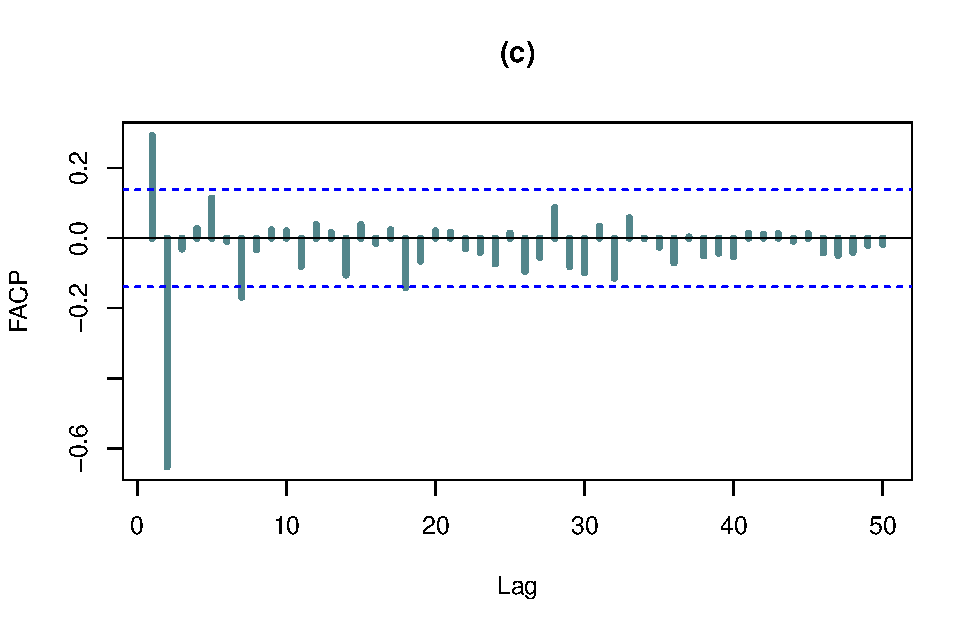
\includegraphics[width=0.33\linewidth]{03-SeriesTemp_files/figure-latex/ar2-3} \caption{AR(2) simulado com coeficiente $\phi_1=0.5$ e $\phi_1=-0.7$  (a), FACV amostral (b) e FAC amostral (c).}\label{fig:ar2}
\end{figure}

\begin{Shaded}
\begin{Highlighting}[]
\KeywordTok{set.seed}\NormalTok{(}\DecValTok{12322}\NormalTok{)}
\NormalTok{ar3=}\KeywordTok{arima.sim}\NormalTok{(}\DataTypeTok{n=}\DecValTok{200}\NormalTok{,}\DataTypeTok{model=}\KeywordTok{list}\NormalTok{(}\DataTypeTok{ar=}\KeywordTok{c}\NormalTok{(}\FloatTok{0.5}\NormalTok{,}\OperatorTok{-}\FloatTok{0.7}\NormalTok{,}\FloatTok{0.6}\NormalTok{)))}
\KeywordTok{plot}\NormalTok{(ar3,}\DataTypeTok{type=}\StringTok{"l"}\NormalTok{,}\DataTypeTok{lwd=}\DecValTok{2}\NormalTok{,}\DataTypeTok{cex.lab=}\FloatTok{1.4}\NormalTok{, }\DataTypeTok{xlab=}\StringTok{" tempo"}\NormalTok{,}\DataTypeTok{ylab=}\StringTok{""}\NormalTok{, }\DataTypeTok{main=}\StringTok{"(a)"}\NormalTok{, }\DataTypeTok{cex.main=}\FloatTok{1.7}\NormalTok{,}\DataTypeTok{col=}\StringTok{"cadetblue4"}\NormalTok{)}
\KeywordTok{acf}\NormalTok{(ar3,}\DataTypeTok{type =} \StringTok{"correlation"}\NormalTok{,}\DataTypeTok{lag.max =} \DecValTok{50}\NormalTok{,}\DataTypeTok{cex.main=}\FloatTok{1.7}\NormalTok{,}\DataTypeTok{col=}\StringTok{"cadetblue4"}\NormalTok{,}\DataTypeTok{ylab=}\StringTok{"FAC"}\NormalTok{,}\DataTypeTok{lwd=}\DecValTok{4}\NormalTok{,}\DataTypeTok{main=}\StringTok{"(b)"}\NormalTok{)}
\KeywordTok{acf}\NormalTok{(ar3,}\DataTypeTok{type =} \StringTok{"partial"}\NormalTok{ ,}\DataTypeTok{lag.max =} \DecValTok{50}\NormalTok{,}\DataTypeTok{cex.main=}\FloatTok{1.7}\NormalTok{,}\DataTypeTok{col=}\StringTok{"cadetblue4"}\NormalTok{,}\DataTypeTok{ylab=}\StringTok{"FACP"}\NormalTok{,}\DataTypeTok{lwd=}\DecValTok{4}\NormalTok{,}\DataTypeTok{main=}\StringTok{"(c)"}\NormalTok{)}
\end{Highlighting}
\end{Shaded}

\begin{figure}
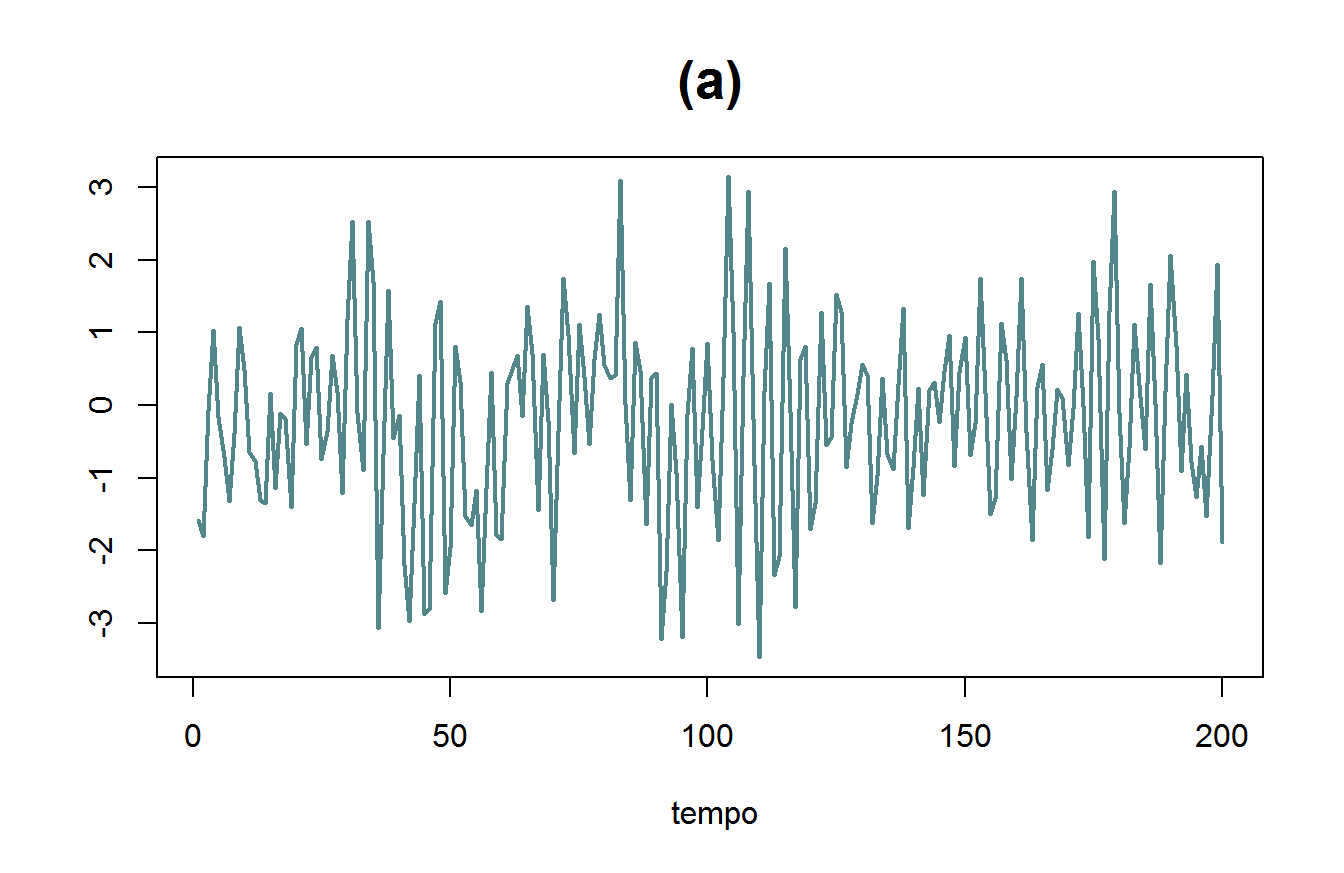
\includegraphics[width=0.33\linewidth]{03-SeriesTemp_files/figure-latex/ar3-1} 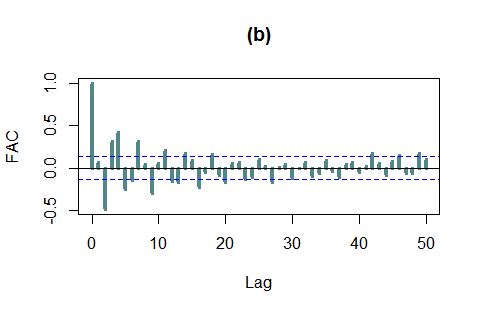
\includegraphics[width=0.33\linewidth]{03-SeriesTemp_files/figure-latex/ar3-2} 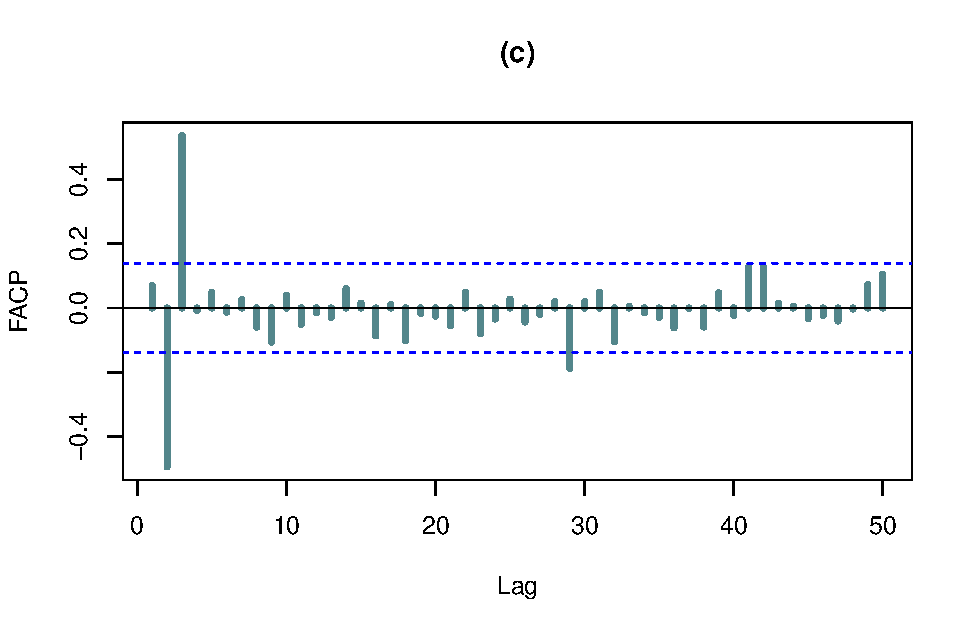
\includegraphics[width=0.33\linewidth]{03-SeriesTemp_files/figure-latex/ar3-3} \caption{AR(3) simulado com coeficiente $\phi_1=0.5$, $\phi_2=-0.7$ e $\phi_3=0.6$   (a), FACV amostral (b) e FAC amostral (c).}\label{fig:ar3}
\end{figure}

\hypertarget{modelo-de-muxe9dias-muxf3veis-maq}{%
\subsection{\texorpdfstring{Modelo de médias-móveis, MA(\emph{q})}{Modelo de médias-móveis, MA(q)}}\label{modelo-de-muxe9dias-muxf3veis-maq}}

Chamamos de médias-móveis de ordem \(q\) o processo definido por:

\begin{center}\rule{0.5\linewidth}{0.5pt}\end{center}

\begin{quote}
\textbackslash textcolor\{blue\}\{ O processo MA(\emph{q})\}\\
\[
Y_t= \varepsilon_t + \theta_1 \varepsilon_{t-1} + \theta_2 \varepsilon_{t-2} +\cdots + \theta_q \varepsilon_{t-q}
\]
em que \(\varepsilon_t\) é um \(RB(0,\sigma_\varepsilon^2)\).
\end{quote}

\begin{center}\rule{0.5\linewidth}{0.5pt}\end{center}

Esta terminologia vem do fato que \(Y_t\) é obtido aplicando-se os pesos \(1,-\theta_1, -\theta_2, \cdots, -\theta_q\), às variáveis \(\varepsilon_t - \varepsilon_{t-1} - \varepsilon_{t-2} -\cdots - \varepsilon_{t-q}\) e então movendo os mesmos pesos 1 unidade do tempo a frente e aplicando-lhes a \(\varepsilon_{t+1} - \varepsilon_{t} - \varepsilon_{t-1} -\cdots - \varepsilon_{t-q+1}\) para obter \(Y_{t+1}\).

Usando o operador \(L\), podemos reescrever o modelo MA(\(q\)) como

\begin{equation}
Y_t= \Theta_q(L)\varepsilon_t,
\label{eq:maqL}
\end{equation}

\begin{equation}
\Theta_q(L)=1+ \theta_1L + \theta_2L^2  +\cdots + \theta_qL^q.
\label{eq:ThetaL}
\end{equation}

\hypertarget{o-modelo-ma1}{%
\subsection{O modelo MA(1)}\label{o-modelo-ma1}}

Para \(q=1\), obtemos o modelo:
\begin{equation}
Y_t = \varepsilon_t + \theta_1 \varepsilon_{t-1},
\label{eq:ma1}
\end{equation}
onde \(\varepsilon_t\) é um \(RB(0,\sigma_\varepsilon^2)\). Segue que

\begin{center}\rule{0.5\linewidth}{0.5pt}\end{center}

\begin{quote}
\textcolor{blue}{ Média do MA(1)}\\
\[\mathbb{E} (Y_t ) = \mathbb{E}(\varepsilon_t + \theta_1 \varepsilon_{t-1})=\mathbb{E}(\varepsilon_t) + \theta_1 \mathbb{E}(\varepsilon_{t-1})=0.\]
\end{quote}

\begin{center}\rule{0.5\linewidth}{0.5pt}\end{center}

\begin{center}\rule{0.5\linewidth}{0.5pt}\end{center}

\begin{quote}
\textcolor{blue}{A variância do MA(1)}\\
\[\mbox{Var}(Y_t )=\mbox{Var}(\varepsilon_t + \theta_1 \varepsilon_{t-1} )= \sigma_\varepsilon^2+\theta_1^2\sigma_\varepsilon^2=(1+\theta_1^2)\sigma_\varepsilon^2.\]
\end{quote}

\begin{center}\rule{0.5\linewidth}{0.5pt}\end{center}

Temos ainda que a função de autocovariância de \emph{lag} \emph{h} é:

\begin{center}\rule{0.5\linewidth}{0.5pt}\end{center}

\begin{quote}
\textbackslash textcolor\{blue\}\{ \emph{FACV} do MA(1)\}
\begin{eqnarray*}
\gamma(h) &=& \mbox{Cov}(Y_t , Y_{t+h} )\\
&=& \mbox{Cov}(\varepsilon_t + \theta_1 \varepsilon_{t-1}, \varepsilon_{t+h} + \theta_1 \varepsilon_{t+h-1} )\\
&=& \mbox{Cov}(\varepsilon_t,\varepsilon_{t+h})+\theta_1\mbox{Cov}(\varepsilon_{t}, \varepsilon_{t+h-1})+\theta_1\mbox{Cov}(\varepsilon_{t-1}, \varepsilon_{t+h})+\theta_1^2\mbox{Cov}(\varepsilon_{t-1}, \varepsilon_{t+h-1})\\
&=&\gamma_\varepsilon(h)+\theta_1\gamma_\varepsilon(h-1)+\theta_1\gamma_\varepsilon(h+1)+\theta_1^2\gamma_\varepsilon(h).
\end{eqnarray*}
\end{quote}

\begin{center}\rule{0.5\linewidth}{0.5pt}\end{center}

Neste caso \(\gamma(h)\) só é diferente de 0 quando algum dos argumentos de \(\gamma_\varepsilon\) for igual a 0, o que acontece somente quando \(h=0\) ou \(h=1\) ou \(h=-1\). Para \(h=0\) obtemos a variância. Para \(h=1\) e \(h=-1\) obtemos \(\gamma(1)=\gamma(-1)=\theta_1\) e para \(|h| \geq 2\) teremos \(\gamma(h) = 0\).
Desta forma,

\begin{center}\rule{0.5\linewidth}{0.5pt}\end{center}

\begin{quote}
\textbackslash textcolor\{blue\}\{ \emph{FACV} \emph{FAC} e do MA(1)\}
\[
\gamma(h)=\begin{cases}
(1+\theta_1^2)\sigma_\varepsilon^2 &\mbox{  se  }\,\,\,\,\,  h=0;\\
\theta_1&\mbox{  se  }\,\,\,\,\,  |k|=1;\\
0&\mbox{  se  }\,\,\,\,\,  |k|\geq 2,\\
\end{cases}\qquad
\rho(h)=\begin{cases}
1&\mbox{  se  }\,\,\,\,\,  k=0;\\
\frac{\theta}{1+\theta^2}&\mbox{  se  }\,\,\,\,\,  |k|=1;\\
0&\mbox{  se  }\,\,\,\,\,  |k|\geq 2.\\
\end{cases}
\]
\end{quote}

\begin{center}\rule{0.5\linewidth}{0.5pt}\end{center}

\hypertarget{propriedades-do-modelo-maq}{%
\subsection{\texorpdfstring{Propriedades do modelo MA(\(q\))}{Propriedades do modelo MA(q)}}\label{propriedades-do-modelo-maq}}

Seja \(\varepsilon_t\sim RB(0,\sigma_\varepsilon^2)\) e considere o modelo MA\((q)\)
\[ Y_t= \varepsilon_t + \theta_1 \varepsilon_{t-1} + \theta_2 \varepsilon_{t-2} +\cdots+ \theta_q \varepsilon_{t-q}.\]
Definindo \(\theta_0=1\), podemos reescrever o modelo MA\((q)\) compactamente como
\[ Y_t= \sum_{k=0}^q \theta_k\varepsilon_{t-k}.\]

A partir daí podemos obter facilmente a média e a variância de \(Y_t\), assim como sua estrutura de autocovariancia e autocorrelação. Primeiramente

\begin{center}\rule{0.5\linewidth}{0.5pt}\end{center}

\begin{quote}
\textbackslash textcolor\{blue\}\{ Média do MA(\emph{q})\}
\[\mathbb{E} (Y_t ) = \mathbb{E}\Big(\sum_{k=0}^q \theta_k\varepsilon_{t-k}\Big)=\sum_{k=0}^q \theta_k\mathbb{E}(\varepsilon_{t-k})= 0\]
\end{quote}

\begin{center}\rule{0.5\linewidth}{0.5pt}\end{center}

\begin{center}\rule{0.5\linewidth}{0.5pt}\end{center}

\begin{quote}
\textbackslash textcolor\{blue\}\{A variância do MA(\emph{q})\}\\
\begin{eqnarray*}
\mbox{Var}(Y_t) &=& \mbox{Var}\Big(\sum_{k=0}^q \theta_k\varepsilon_{t-k}\Big) = \sum_{k=0}^q \theta_k^2\mbox{Var}(\varepsilon_{t-k}) = \sigma_\varepsilon^2\sum_{k=0}^q \theta_k^2\\
&=& (1 + \theta_1^2 +\cdots +\theta_q^2)\sigma_\varepsilon^2.
\end{eqnarray*}
------------------------------------------------------------
\end{quote}

\begin{center}\rule{0.5\linewidth}{0.5pt}\end{center}

\begin{quote}
\textbackslash textcolor\{blue\}\{ \emph{FACV} do MA(\emph{q})\}
\begin{align*}
\gamma(h)&=\mbox{Cov}(Y_t,Y_{t-h} )\\
&= \mbox{Cov}\Big(\sum_{k=0}^q \theta_k\varepsilon_{t-k},\sum_{j=0}^q \theta_j\varepsilon_{t-h-j}\Big)\\
&=\sum_{k=0}^q \sum_{j=0}^q\theta_k\theta_j\mbox{Cov}(\varepsilon_{t-k},\varepsilon_{t-h-j})\\
&=\sum_{k=0}^q \sum_{j=0}^q\theta_k\theta_j\gamma_\varepsilon(k-h-j)
\end{align*}
note que \(\gamma_\varepsilon(k-h-j)\neq 0\) somente quando \(k-h-j=0\), ou seja, se \(j=k-h\).
\end{quote}

\begin{center}\rule{0.5\linewidth}{0.5pt}\end{center}

Além disso, se \(|h|>q\), não é possível acontecer \(k-h-j=0\). Desta forma, se \(|h|\leq q\),

\[  \gamma(h)=\sum_{k=0}^q \theta_k\theta_{k-h}\gamma_\varepsilon(0)=\sigma_\varepsilon^2\sum_{k=0}^q \theta_k\theta_{k-h}.\]
Concluimos que

\begin{center}\rule{0.5\linewidth}{0.5pt}\end{center}

\begin{quote}
\textbackslash textcolor\{blue\}\{ \emph{FACV} e \emph{FAC} do MA(\emph{q})\}
\[\gamma(h)=\left\{
\begin{array}{cc}
\sigma_\varepsilon^2\displaystyle{\sum_{k=0}^q \theta_k\theta_{k-h}},  & \mbox{ se } |h|\leq q;\\
0, &  \mbox{ se } |h|> q,
\end{array}
\right. \quad \mbox{ e } \quad \rho(h)=\left\{
\begin{array}{cc}
\displaystyle{\frac{\sum_{k=0}^q \theta_k\theta_{k-h}}{\sum_{j=0}^q \theta_j^2}},  & \mbox{ se } |h|\leq q;\quad\\
0, &  \mbox{ se } |h|> q.
\end{array}\right.\]
\end{quote}

\begin{center}\rule{0.5\linewidth}{0.5pt}\end{center}

\begin{Shaded}
\begin{Highlighting}[]
\CommentTok{# MA(1) Simulado}
\KeywordTok{set.seed}\NormalTok{(}\DecValTok{12322}\NormalTok{)}
\NormalTok{ma1_}\DecValTok{1}\NormalTok{=}\KeywordTok{arima.sim}\NormalTok{(}\DataTypeTok{n=}\DecValTok{200}\NormalTok{,}\DataTypeTok{model=}\KeywordTok{list}\NormalTok{(}\DataTypeTok{ma=}\KeywordTok{c}\NormalTok{(}\DecValTok{1}\NormalTok{)))}
\KeywordTok{plot}\NormalTok{(ma1_}\DecValTok{1}\NormalTok{,}\DataTypeTok{type=}\StringTok{"l"}\NormalTok{,}\DataTypeTok{lwd=}\DecValTok{2}\NormalTok{,}\DataTypeTok{cex.lab=}\FloatTok{1.4}\NormalTok{, }\DataTypeTok{xlab=}\StringTok{" tempo"}\NormalTok{,}\DataTypeTok{ylab=}\StringTok{""}\NormalTok{, }\DataTypeTok{main=}\StringTok{"(a)"}\NormalTok{, }\DataTypeTok{cex.main=}\FloatTok{1.7}\NormalTok{,}\DataTypeTok{col=}\StringTok{"cadetblue4"}\NormalTok{)}
\KeywordTok{acf}\NormalTok{(ma1_}\DecValTok{1}\NormalTok{,}\DataTypeTok{type =} \StringTok{"correlation"}\NormalTok{,}\DataTypeTok{lag.max =} \DecValTok{50}\NormalTok{,}\DataTypeTok{cex.main=}\FloatTok{1.7}\NormalTok{,}\DataTypeTok{col=}\StringTok{"cadetblue4"}\NormalTok{,}\DataTypeTok{ylab=}\StringTok{"FAC"}\NormalTok{,}\DataTypeTok{lwd=}\DecValTok{4}\NormalTok{,}\DataTypeTok{main=}\StringTok{"(b)"}\NormalTok{)}
\KeywordTok{acf}\NormalTok{(ma1_}\DecValTok{1}\NormalTok{,}\DataTypeTok{type =} \StringTok{"partial"}\NormalTok{ ,}\DataTypeTok{lag.max =} \DecValTok{50}\NormalTok{,}\DataTypeTok{cex.main=}\FloatTok{1.7}\NormalTok{,}\DataTypeTok{col=}\StringTok{"cadetblue4"}\NormalTok{,}\DataTypeTok{ylab=}\StringTok{"FACP"}\NormalTok{,}\DataTypeTok{lwd=}\DecValTok{4}\NormalTok{,}\DataTypeTok{main=}\StringTok{"(c)"}\NormalTok{)}
\end{Highlighting}
\end{Shaded}

\begin{figure}
\includegraphics[width=0.33\linewidth]{03-SeriesTemp_files/figure-latex/ma11-1} \includegraphics[width=0.33\linewidth]{03-SeriesTemp_files/figure-latex/ma11-2} \includegraphics[width=0.33\linewidth]{03-SeriesTemp_files/figure-latex/ma11-3} \caption{MA(1) simulado com coeficiente $\theta_1=1$, (a) FACV amostral (b) e FAC amostral (c).}\label{fig:ma11}
\end{figure}

\begin{Shaded}
\begin{Highlighting}[]
\CommentTok{# MA(1) Simulado}
\KeywordTok{set.seed}\NormalTok{(}\DecValTok{12322}\NormalTok{)}
\NormalTok{ma1_m08=}\KeywordTok{arima.sim}\NormalTok{(}\DataTypeTok{n=}\DecValTok{200}\NormalTok{,}\DataTypeTok{model=}\KeywordTok{list}\NormalTok{(}\DataTypeTok{ma=}\KeywordTok{c}\NormalTok{(}\OperatorTok{-}\FloatTok{0.8}\NormalTok{)))}
\KeywordTok{plot}\NormalTok{(ma1_m08,}\DataTypeTok{type=}\StringTok{"l"}\NormalTok{,}\DataTypeTok{lwd=}\DecValTok{2}\NormalTok{,}\DataTypeTok{cex.lab=}\FloatTok{1.4}\NormalTok{, }\DataTypeTok{xlab=}\StringTok{" tempo"}\NormalTok{,}\DataTypeTok{ylab=}\StringTok{""}\NormalTok{, }\DataTypeTok{main=}\StringTok{"(a)"}\NormalTok{, }\DataTypeTok{cex.main=}\FloatTok{1.7}\NormalTok{,}\DataTypeTok{col=}\StringTok{"cadetblue4"}\NormalTok{)}
\KeywordTok{acf}\NormalTok{(ma1_m08,}\DataTypeTok{type =} \StringTok{"correlation"}\NormalTok{,}\DataTypeTok{lag.max =} \DecValTok{50}\NormalTok{,}\DataTypeTok{cex.main=}\FloatTok{1.7}\NormalTok{,}\DataTypeTok{col=}\StringTok{"cadetblue4"}\NormalTok{,}\DataTypeTok{ylab=}\StringTok{"FAC"}\NormalTok{,}\DataTypeTok{lwd=}\DecValTok{4}\NormalTok{,}\DataTypeTok{main=}\StringTok{"(b)"}\NormalTok{)}
\KeywordTok{acf}\NormalTok{(ma1_m08,}\DataTypeTok{type =} \StringTok{"partial"}\NormalTok{ ,}\DataTypeTok{lag.max =} \DecValTok{50}\NormalTok{,}\DataTypeTok{cex.main=}\FloatTok{1.7}\NormalTok{,}\DataTypeTok{col=}\StringTok{"cadetblue4"}\NormalTok{,}\DataTypeTok{ylab=}\StringTok{"FACP"}\NormalTok{,}\DataTypeTok{lwd=}\DecValTok{4}\NormalTok{,}\DataTypeTok{main=}\StringTok{"(c)"}\NormalTok{)}
\end{Highlighting}
\end{Shaded}

\begin{figure}
\includegraphics[width=0.33\linewidth]{03-SeriesTemp_files/figure-latex/ma1m08-1} \includegraphics[width=0.33\linewidth]{03-SeriesTemp_files/figure-latex/ma1m08-2} \includegraphics[width=0.33\linewidth]{03-SeriesTemp_files/figure-latex/ma1m08-3} \caption{MA(1) simulado com coeficiente $\theta_1=-0.8$, (a) FACV amostral (b) e FAC amostral (c).}\label{fig:ma1m08}
\end{figure}

\begin{Shaded}
\begin{Highlighting}[]
\CommentTok{# MA(1) Simulado}
\KeywordTok{set.seed}\NormalTok{(}\DecValTok{1234}\NormalTok{)}
\NormalTok{ma1_m0804=}\KeywordTok{arima.sim}\NormalTok{(}\DataTypeTok{n=}\DecValTok{300}\NormalTok{,}\DataTypeTok{model=}\KeywordTok{list}\NormalTok{(}\DataTypeTok{ma=}\KeywordTok{c}\NormalTok{(}\OperatorTok{-}\FloatTok{0.8}\NormalTok{,}\FloatTok{0.4}\NormalTok{)))}
\KeywordTok{plot}\NormalTok{(ma1_m0804,}\DataTypeTok{type=}\StringTok{"l"}\NormalTok{,}\DataTypeTok{lwd=}\DecValTok{2}\NormalTok{,}\DataTypeTok{cex.lab=}\FloatTok{1.4}\NormalTok{, }\DataTypeTok{xlab=}\StringTok{" tempo"}\NormalTok{,}\DataTypeTok{ylab=}\StringTok{""}\NormalTok{, }\DataTypeTok{main=}\StringTok{"(a)"}\NormalTok{, }\DataTypeTok{cex.main=}\FloatTok{1.7}\NormalTok{,}\DataTypeTok{col=}\StringTok{"cadetblue4"}\NormalTok{)}
\KeywordTok{acf}\NormalTok{(ma1_m0804,}\DataTypeTok{type =} \StringTok{"correlation"}\NormalTok{,}\DataTypeTok{lag.max =} \DecValTok{50}\NormalTok{,}\DataTypeTok{cex.main=}\FloatTok{1.7}\NormalTok{,}\DataTypeTok{col=}\StringTok{"cadetblue4"}\NormalTok{,}\DataTypeTok{ylab=}\StringTok{"FAC"}\NormalTok{,}\DataTypeTok{lwd=}\DecValTok{4}\NormalTok{,}\DataTypeTok{main=}\StringTok{"(b)"}\NormalTok{)}
\KeywordTok{acf}\NormalTok{(ma1_m0804,}\DataTypeTok{type =} \StringTok{"partial"}\NormalTok{ ,}\DataTypeTok{lag.max =} \DecValTok{50}\NormalTok{,}\DataTypeTok{cex.main=}\FloatTok{1.7}\NormalTok{,}\DataTypeTok{col=}\StringTok{"cadetblue4"}\NormalTok{,}\DataTypeTok{ylab=}\StringTok{"FACP"}\NormalTok{,}\DataTypeTok{lwd=}\DecValTok{4}\NormalTok{,}\DataTypeTok{main=}\StringTok{"(c)"}\NormalTok{)}
\end{Highlighting}
\end{Shaded}

\begin{figure}
\includegraphics[width=0.33\linewidth]{03-SeriesTemp_files/figure-latex/ma1m0804-1} \includegraphics[width=0.33\linewidth]{03-SeriesTemp_files/figure-latex/ma1m0804-2} \includegraphics[width=0.33\linewidth]{03-SeriesTemp_files/figure-latex/ma1m0804-3} \caption{MA(2) simulado com coeficiente $\theta_1=-0.8$ e $\theta_1=0.4$, (a) FACV amostral (b) e FAC amostral (c).}\label{fig:ma1m0804}
\end{figure}

\begin{Shaded}
\begin{Highlighting}[]
\CommentTok{# MA(1) Simulado}
\KeywordTok{set.seed}\NormalTok{(}\DecValTok{12341}\NormalTok{)}
\NormalTok{ma1_m080414=}\KeywordTok{arima.sim}\NormalTok{(}\DataTypeTok{n=}\DecValTok{300}\NormalTok{,}\DataTypeTok{model=}\KeywordTok{list}\NormalTok{(}\DataTypeTok{ma=}\KeywordTok{c}\NormalTok{(}\OperatorTok{-}\FloatTok{0.8}\NormalTok{,}\FloatTok{0.4}\NormalTok{,}\FloatTok{1.4}\NormalTok{)))}
\KeywordTok{plot}\NormalTok{(ma1_m080414,}\DataTypeTok{type=}\StringTok{"l"}\NormalTok{,}\DataTypeTok{lwd=}\DecValTok{2}\NormalTok{,}\DataTypeTok{cex.lab=}\FloatTok{1.4}\NormalTok{, }\DataTypeTok{xlab=}\StringTok{" tempo"}\NormalTok{,}\DataTypeTok{ylab=}\StringTok{""}\NormalTok{, }\DataTypeTok{main=}\StringTok{"(a)"}\NormalTok{, }\DataTypeTok{cex.main=}\FloatTok{1.7}\NormalTok{,}\DataTypeTok{col=}\StringTok{"cadetblue4"}\NormalTok{)}
\KeywordTok{acf}\NormalTok{(ma1_m080414,}\DataTypeTok{type =} \StringTok{"correlation"}\NormalTok{,}\DataTypeTok{lag.max =} \DecValTok{50}\NormalTok{,}\DataTypeTok{cex.main=}\FloatTok{1.7}\NormalTok{,}\DataTypeTok{col=}\StringTok{"cadetblue4"}\NormalTok{,}\DataTypeTok{ylab=}\StringTok{"FAC"}\NormalTok{,}\DataTypeTok{lwd=}\DecValTok{4}\NormalTok{,}\DataTypeTok{main=}\StringTok{"(b)"}\NormalTok{)}
\KeywordTok{acf}\NormalTok{(ma1_m080414,}\DataTypeTok{type =} \StringTok{"partial"}\NormalTok{ ,}\DataTypeTok{lag.max =} \DecValTok{50}\NormalTok{,}\DataTypeTok{cex.main=}\FloatTok{1.7}\NormalTok{,}\DataTypeTok{col=}\StringTok{"cadetblue4"}\NormalTok{,}\DataTypeTok{ylab=}\StringTok{"FACP"}\NormalTok{,}\DataTypeTok{lwd=}\DecValTok{4}\NormalTok{,}\DataTypeTok{main=}\StringTok{"(c)"}\NormalTok{)}
\end{Highlighting}
\end{Shaded}

\begin{figure}
\includegraphics[width=0.33\linewidth]{03-SeriesTemp_files/figure-latex/ma1m080414-1} \includegraphics[width=0.33\linewidth]{03-SeriesTemp_files/figure-latex/ma1m080414-2} \includegraphics[width=0.33\linewidth]{03-SeriesTemp_files/figure-latex/ma1m080414-3} \caption{MA(2) simulado com coeficiente $\theta_1=-0.8$, $\theta_1=0.4$ e $\theta_1=1.4$, (a) FACV amostral (b) e FAC amostral (c).}\label{fig:ma1m080414}
\end{figure}

\hypertarget{modelo-armapq}{%
\subsection{\texorpdfstring{Modelo ARMA(\(p\),\(q\))}{Modelo ARMA(p,q)}}\label{modelo-armapq}}

Um modelo mais geral é dado pela aglutinação dos modelos AR e MA em um único modelos, ao qual chamamos Modelos Autoregressivos de Média Móveis, abreviado ARMA. Um processo \(\{Y_t\}_t\) é um ARMA\((p,q)\) se pode ser escrito como

onde \(\varepsilon_t\sim RB(0,\sigma_\varepsilon^2)\), \(\phi_1,\cdots,\phi_p\in\mathbb{R}\) são os coeficientes da parte AR e \(\theta_1,\cdots\theta_q\in\mathbb{R}\) são os coeficientes da parte MA do processo. Utilizando os polinômios AR e MA vistos anteriormente, podemos escrever um processo ARMA\((p,q)\) de uma forma compacta e elegante.

\begin{center}\rule{0.5\linewidth}{0.5pt}\end{center}

\begin{quote}
\textbackslash textcolor\{blue\}\{ O modelo ARMA(\emph{p},\emph{q})\}
\begin{equation}
Y_t=\phi_1Y_{t-1}+\cdots+\phi_pY_{t-p}+\theta_1\varepsilon_{t-1}+\cdots+\theta_q\varepsilon_{t-q} + \varepsilon_t
\label{eq:mARMA2}
\end{equation}
em que \(\varepsilon_t\sim RB(0,\sigma_\varepsilon^2)\), \(\phi_1,\cdots,\phi_p\in\mathbb{R}\) são os coeficientes da parte AR e \(\theta_1,\cdots\theta_q\in\mathbb{R}\) são os coeficientes da parte MA do processo.
\end{quote}

\begin{center}\rule{0.5\linewidth}{0.5pt}\end{center}

Utilizando os polinômios AR e MA vistos anteriormente, podemos escrever um processo ARMA\((p,q)\) de uma forma compacta e elegante.

\[\Phi_p(L)Y_t=\Theta_q(L)\varepsilon_t,\]
em que \(\varepsilon_t\) é um \(RB(0,\sigma_\varepsilon^2)\), \(\Phi_p(L)\) e \(\Theta_p(L)\) são polinômios da parte AR e MA (respectivamente) dados por
\[\Phi_p(L)=1-\phi_1L-\phi_2L^ 2-\cdots-\phi_pL^p  \quad\mbox{e}\quad  \Theta_q(L)=1+ \theta_1L + \theta_2L^2  +\cdots + \theta_qL^q.\]

\begin{example}[ Modelo ARMA(2,3) ]
\protect\hypertarget{exm:arma23}{}{\label{exm:arma23} \iffalse ( Modelo ARMA(2,3) ) \fi{} }O Modelo ARMA(2,3) é escrito como

\begin{eqnarray*}
\Phi_2(L)y_t&=&\Psi_3(L)\varepsilon_t\\
(1-\phi_1L-\phi_2L^2)y_t&=&(1+\theta_1L+\theta_2L^2+\theta_3L^3)\varepsilon_t\\
y_t&=&\phi_1y_{t-1}+\phi_2y_{t-2}+\varepsilon_t+\theta_1\varepsilon_{t-1}+\theta_2\varepsilon_{t-2}+\theta_3\varepsilon_{t-3}.
\end{eqnarray*}
\end{example}

\hypertarget{exemplos-arma-simulados}{%
\subsubsection{Exemplos ARMA simulados}\label{exemplos-arma-simulados}}

\begin{example}[Causalidade do processo AR(1)]
\protect\hypertarget{exm:causar1}{}{\label{exm:causar1} \iffalse (Causalidade do processo AR(1)) \fi{} }O modelo AR(1):

\[
y_t = \phi y_{t-1} + e_t,
\]

pode ser escrito como
\[
 y_t = e_t + \phi e_{t-1} + \phi^2 e_{t-2} + \cdots + \phi^{k-1}e_{t-(k-1)} + \phi^ky_{t-k},
\]
em que para \(k\) grande tem-se

\begin{eqnarray*}
y_t & = & e_t + \phi e_{t-1} + \phi^2 e_{t-2} + \ldots\\
   & = & \psi_0 e_t + \psi_1 e_{t-1} + \psi_2 e_{t-2} + \ldots,
\end{eqnarray*}
em que \(|\phi| < 1\) e \(\psi_j = \phi^j\). O que acontece com a variância de \(y_t\)? Assim, essa representação somente faz sentido se
\(\sum_{j=0}^{\infty}\psi_j<\infty\), o que ocorre se, e somente se, \(|\phi|<1\).
\end{example}

\hypertarget{causalidade}{%
\subsection{Causalidade}\label{causalidade}}

O conceito de \textcolor{blue}{ causalidade } consiste em escrever um processo AR(\(q\)) como um MA(\(\infty\)).

\begin{center}\rule{0.5\linewidth}{0.5pt}\end{center}

\begin{quote}
Um processo linear \(\{Y_t \}\) é \textcolor{blue}{ CAUSAL } (estritamente, uma função causal de \(\{\varepsilon_t \}\)) se existem reais \(\psi_0,\psi_1,\cdots\) satisfazendo \(\sum_{j=0}^{\infty}|\psi_j|<\infty\) e tais que
\begin{align}
Y_t = \psi_0\varepsilon_t + \psi_1\varepsilon_{t-1} + \psi_2 \varepsilon_{t-2} + \cdots = \sum_{k=0}^\infty\psi_k\varepsilon_{t-k}= \Psi(L)\varepsilon_t,
\label{eq:causaldef}
\end{align}
onde denotamos
\[
\Psi(L) = \psi_0 + \psi_1 L + \psi_2 L^2 + \cdots = \sum_{k=0}^\infty\psi_kL^k.
\]
\end{quote}

\begin{center}\rule{0.5\linewidth}{0.5pt}\end{center}

O modelo AR(1) é dado por:

\[
Y_t = \phi Y_{t-1} + \varepsilon_t,
\]
para \(|\phi|<1\) e \(\varepsilon_t\sim RB(0,\sigma^2_\varepsilon)\). Na Seção \ref{sec:subar1} obtivemos a representação (com \(c=0\))
\[Y_t = \sum_{j=0}^\infty \phi^j\varepsilon_{t-j}.\]
Identificando-se \(\psi_j= \phi^j\), obtemos que \(Y_t\) possui a representação \eqref{eq:causaldef} e observando que, como \(|\phi|<1\),
\[\sum_{j=0}^{\infty}|\psi_j|=\sum_{j=0}^{\infty}|\phi|^j=\frac1{1-|\phi|}<\infty,\]
segue que um AR(1) com \(|\phi|<1\) é causal.

Obviamente todo modelo MA\((q)\) é causal, dado que se
\[Y_t=\varepsilon_t+\theta\varepsilon_{t-1}+\cdots+\theta_q\varepsilon_{t-q},\]
com \(\varepsilon_t\sim RB(0, \sigma_\varepsilon^2)\), tomamos \(\psi_0=1\), \(\psi_j=\theta_j\), para \(j=1,\cdots,q\) e \(\psi_j=0\) para \(j>q\), temos que a representação \eqref{eq:causaldef} é satisfeita e, evidentemente, \(\sum_{j=0}^\infty|\psi|_j=1+|\theta_1|+\cdots+|\theta_q|<\infty\).

\hypertarget{invertibilidade}{%
\subsection{Invertibilidade}\label{invertibilidade}}

Mostramos que um processo AR pode ser reescrito como um processo MA de ordem infinita através de pesos \(\psi_j\)'s. Podemos nos perguntar quando (e se) é possível escrever um processo MA como
um autorregressivo.

\begin{center}\rule{0.5\linewidth}{0.5pt}\end{center}

\begin{quote}
Um processo linear \(\{Y_t \}\) é dito ser \textcolor{blue}{ INVERTÍVEL } (estritamennte, uma função invertível de \(\{\varepsilon_t \}\)) se existem reais \(\mbox{Var}phi_1,\mbox{Var}phi_2,\cdots\) satisfazendo \(\sum_{j=0}^{\infty}|\mbox{Var}phi_j|<\infty\) e tais que
\begin{align}
\varepsilon_t = \mbox{Var}phi_0Y_t+\mbox{Var}phi_1Y_{t-1}+\mbox{Var}phi_2Y_{t-2}+\cdots =\sum_{k=0}^\infty\mbox{Var}phi_kY_{t-k}=\Phi(L)Y_t,
\label{eq:invertdef}
\end{align}
onde denotamos
\[
\Phi(L) = \mbox{Var}phi_0 + \mbox{Var}phi_1 L + \mbox{Var}phi_2 L^2 + \cdots = \sum_{k=0}^\infty\mbox{Var}phi_kL^k.
\]
\end{quote}

\begin{center}\rule{0.5\linewidth}{0.5pt}\end{center}

\begin{example}[Invertibilidade do processo MA(1)]
\protect\hypertarget{exm:invma1}{}{\label{exm:invma1} \iffalse (Invertibilidade do processo MA(1)) \fi{} }Considere o modelo MA(1)

\[
Y_t = \varepsilon_t -\theta \varepsilon_{t-1},
\]
em que \(\varepsilon_t\) é um \(RB(0,\sigma^2)\). Reescrevendo a equação acima
como
\[
\varepsilon_t = Y_t + \theta \varepsilon_{t-1}
\]
e substituindo \(t\) por \(t - 1\)
e \(\varepsilon_{t-1}\) na equação modificada, temos:
\begin{eqnarray*}
\varepsilon_t &=& Y_t + \theta(Y_{t-1} + \theta \varepsilon_{t-2})\\
    &=& Y_t + \theta Y_{t-1} + \theta^2Y_{t-2}
\end{eqnarray*}
Se \(|\theta| < 1\), podemos continuar a substituição e obter:
\begin{eqnarray*}
  \varepsilon_t  &=& Y_t + \theta Y_{t-1} + \theta^2Y_{t-2}+\cdots = \sum_{j=0}^\infty\theta^jY_{t-j}.
\end{eqnarray*}

Assim, da mesma forma como foi feito para o AR(1), tomando \(\mbox{Var}\phi_j=\theta^j\), segue que, se \(|\theta| < 1\), a representação \eqref{invert_def} é satisfeita e \(\sum_{j=0}^\infty|\mbox{Var}\phi_j|=\frac1{1-|\theta|}<\infty\) de onde concluimos que o modelo MA(1) é invertível. Em outras palavras, um modelo MA(1) pode ser invertido (transformado) para um AR(\(\infty\)), sempre que \(|\theta|<1\).
\end{example}

\hypertarget{polinuxf4mio-caracteruxedstico}{%
\subsection{Polinômio característico}\label{polinuxf4mio-caracteruxedstico}}

Nos exemplos mostrados acima tratamos da causalidade e invertibilidade dos casos
AR(1) e MA(1) em particular. Para os casos mais gerais AR(\(p\)) e MA(\(q\)) utilizamos os
chamados \textbf{\emph{polinômios característicos}} para decidir se os processos são causais e/ou invertíveis.

Para um modelo geral AR(\(p\)), definimos o \textbf{\emph{polinômios característicos AR}}
como
\[
\Phi(z) = 1 - \phi_1 z -\phi_2 z^2-\cdots-\phi_p z^p, \ \ z\in\mathbb{C}
\]

\begin{theorem}
\protect\hypertarget{thm:soluest}{}{\label{thm:soluest} }Uma (única) solução \textbf{estacionária} para \(\Phi(L)y_t = e_t\) existe se, e somente, as raízes de \(\Phi(z)\) \textbf{não pertence ao círculo de raio um}, ou seja,

\begin{equation*}
|z| = 1 \rightarrow \Phi(z) = 1 - \phi_1 z - \cdots - \phi_p z^p \neq 0.
\end{equation*}

O processo AR(\(p\)) é \textbf{causal} se, e somente se as raízes de \(\Phi(z)\) estão \textbf{fora do círculo unitário}, ou seja,

\[
|z| \leq 1 \rightarrow \Phi(z) = 1 - \phi_1 z - \cdots - \phi_p z^p \neq 0.
\]
\end{theorem}

Para um modelo geral MA(\(q\)), definimos o \textcolor{blue}{ polinômio característico MA } como
\begin{equation*}
\Theta(z) = 1 + \theta_1 z +\theta_2 z^2+\cdots+\theta_q z^q.
\end{equation*}

\begin{theorem}
\protect\hypertarget{thm:invert}{}{\label{thm:invert} }Um processo MA(\(q\)) é invertível se, e somente se, as raízes de \(\Theta(z)\) estão fora do círculo
unitário, isto é,

\begin{equation*}
z\in\mathbb{C} : |z|\leq  1 \mathbb{R}ightarrow \Theta(z) = 1 + \theta_1 z +\theta_2 z^2+\cdots+\theta_q z^q\neq 0.
\end{equation*}
\end{theorem}

\begin{remark}
\iffalse{} {Observação. } \fi{}Um processo ARMA será invertível e estacionário se a parte AR o for, e será invertível se a parte MA o for.
\end{remark}

\hypertarget{estacionariedade-e-causalidade-de-um-processo-arma}{%
\subsection{Estacionariedade e causalidade de um processo ARMA}\label{estacionariedade-e-causalidade-de-um-processo-arma}}

Para um processo ARMA, as condições para causalidade, invertibilidade e estacionariedade são dadas no seguinte teorema.

\begin{theorem}
\protect\hypertarget{thm:causaarma}{}{\label{thm:causaarma} }Se \(\Phi(\cdot)\) e \(\Theta(\cdot)\) não possuem fatores em comum, existe
uma única solução estacionária \(\{Y_t\}\) para \(\Phi(L)Y_t = \Theta(L)\varepsilon_t\)
se, e somente se,

\begin{equation*}
z\in\mathbb{C} : |z| = 1 \mathbb{R}ightarrow \Phi(z) = 1 - \phi_1 z - \cdots - \phi_p z^p \neq 0.
\end{equation*}

Esse processo ARMA(\(p,q\)) é causal se, e somente se,
\begin{equation*}
z\in\mathbb{C} : |z| \leq 1 \mathbb{R}ightarrow \Phi(z) = 1 - \phi_1 z - \cdots - \phi_p z^p \neq 0.
\end{equation*}

Será invertível se, e somente se

\begin{equation*}
z\in\mathcal{C} : |z|\leq  1 \mathbb{R}ightarrow \Theta(z) = 1 + \theta_1 z +\theta_2 z^2+\cdots+\theta_q z^q\neq 0.
\end{equation*}
\end{theorem}

\hypertarget{exercuxedcios}{%
\section{Exercícios}\label{exercuxedcios}}

\begin{exercise}
\protect\hypertarget{exr:pest}{}{\label{exr:pest} }Defina processo estocástico e ilustre graficamente. Explique o que é a realização de um processo estocástico e por que séries econômicas podem ser entendidas como geradas por um processo estocásticos.
\end{exercise}

\begin{exercise}
\protect\hypertarget{exr:stce}{}{\label{exr:stce} } Seja \(\{y_t\}^T_{t=1}\) uma série temporal. Quais características essa série deve apresentar para ser considerada uma série de covariância estacionária?
\end{exercise}

\begin{exercise}
\protect\hypertarget{exr:defrb}{}{\label{exr:defrb} }Faça os seguintes items:

~~~a) Defina o que é um processo ruído branco.

~~~b) Defina o que é um processo independente e identicamente distribuído (i.i.d.).

~~~c) Defina ruído branco Gaussiano.

~~~d) Qual a relação entre ruído branco, ruído branco Gaussiano e processo i.i.d.?

~~~e) Esses processos são estacionários?
\end{exercise}

\begin{exercise}
\protect\hypertarget{exr:ma1}{}{\label{exr:ma1} }Considere um processo MA(1):
\(y_t=e_t+\alpha_1e_{t-1};\) onde \(e_t \sim RB(0,\sigma^2_e)\).

~~~a) Calcule a média e variância de \(y_t\).

~~~b) Calcule as autocovariâncias de \(lags\) 1 e 2 para a série \(y_t\).

~~~c) Esse processo é estacionário? (Justifique sua resposta usando os valores encontrados nos itens anteriores juntamente com o conceito de estacionariedade definido na Questão 1).

~~~d) Comente a afirmativa: ``Todo processo MA(\(q\)), onde \(q < \infty,\) é estacionário''.

~~~e) Suponha que \(\alpha_1=0.5\). O processo é invertível?\\
\hspace*{0.333em}\hspace*{0.333em}\hspace*{0.333em}f) Calcule a autocorrelação de ordem 1 para o processo do item anterior e faça o gráfico da FAC com 5 \(lags\).
\end{exercise}

\begin{exercise}
\protect\hypertarget{exr:ma2}{}{\label{exr:ma2} } Considere um processo MA(2): \(y_t=e_t+\alpha_1e_{t-1}+\alpha_2e_{t-2};\) onde \(e_t \sim RB(0,\sigma^2_e)\).

~~~a) Calcule a média e variância de \(y_t\).

~~~b) Calcule as autocovariâncias de \(lags\) 1, 2 e 3 para a série \(y_t\).

~~~c) Esse processo é estacionário? (Justifique sua resposta usando os valores encontrados nos itens anteriores juntamente com o conceito de estacionariedade definido na Questão 1).

~~~d) Suponha que \(\alpha_1=0.65\) e que \(\alpha_2=-0.20\). O processo é invertível?\\
\hspace*{0.333em}\hspace*{0.333em}\hspace*{0.333em}e) Calcule a autocorrelação de ordem 1 e 2 para o processo do item anterior e faça o gráfico da FAC com 5 \(lags\).
\end{exercise}

\begin{exercise}
\protect\hypertarget{exr:p1p2}{}{\label{exr:p1p2} }Considere os seguintes processos
\[y_t=e_t+\theta e_{t-1} \quad\mbox{e} \quad y_t=e_t+\frac{1}{\theta}e_{t-1},\] onde \(e_t \sim iid(0,\sigma^2_e)\) e \(\theta \neq 0\).

~~~a) Os processos acima possuem as mesmas autocorrelações? Verifique.

~~~b) Os processos acima são invertíveis? Verifique.
\end{exercise}

\begin{exercise}
\protect\hypertarget{exr:ar1}{}{\label{exr:ar1} }Considere um processo AR(1):
\(y_t=5+0.9y_{t-1}+e_t\), onde \(e_t \sim RB(0,\sigma^2_e)\).

~~~a) Esse processo é estacionário? Verifique.

~~~b) Calcule as autocorrelações de ordem 1, 2 e 3 para esse processo. Faça um esboço do gráfico da FAC para esse processo com 5 \(lags\).

~~~c) O que significa o coeficiente de \(y_{t-1}\) num processo AR(1)?\\
\hspace*{0.333em}\hspace*{0.333em}\hspace*{0.333em}d) Faça um gráfico da FACP desse processo com 5 \(lags\).
\end{exercise}

```\{exercise ar123\} Para os seguintes itens, responda:

~~~a) Explique como se comportam os gráficos da FAC e da FACP em processos AR(\(p\)) e em processos MA(\(q\)).

~~~b) Esboce os gráficos da FAC e FACP para os seguintes processos: AR(1), AR(3), MA(2) e MA(3).

\begin{verbatim}


<br>

```{exercise exarmafac} Para os seguintes itens, responda:

|    a\) Supondo que $E(y_t)=\mu$ e que $y_t=c_0+\beta_1y_{t-1}+e_t+\alpha_1e_{t-1}$, calcule o valor de $c_0$ em termos de $\mu$ e $\beta_{1}$.

|    b\) Explique como se comportam os gráficos da FAC e da FACP em processos ARMA($p,q$).

|    c\) Esboce os gráficos da FAC e FACP para um processos ARMA(1,1).
\end{verbatim}

\begin{exercise}
\protect\hypertarget{exr:exarmamet}{}{\label{exr:exarmamet} }Explique os passos que devem ser seguidos para a modelagem de uma série temporal na metodologia ARMA.
\end{exercise}

\begin{exercise}[ANPEC 2014-5]
\protect\hypertarget{exr:a145}{}{\label{exr:a145} \iffalse (ANPEC 2014-5) \fi{} }Suponha que \(Y_t\) seja representado pelo seguinte processo autorregressivo de primeira ordem:
\[Y_t = 10 + 0,6 Y_{t-1} + e_t ,\]
em que et é um ruído branco que satisfaz as condições: \(\mathbb{E}(e_t)=0,\) \(\mathbb{E}(e_t^2)=\sigma^2\), \(\mathbb{E}(e_te_s)=0\) para \(t\neq s.\) Suponha também que \(Y_0=0\). Obtenha \(\mathbb{E}(Y_t)\) para \(t=2\).
\end{exercise}

\begin{exercise}[ANPEC 2014-10]
\protect\hypertarget{exr:a1410}{}{\label{exr:a1410} \iffalse (ANPEC 2014-10) \fi{} }Considere o seguinte processo:
\[Y_t=\rho Y_{t-1}+e_t,\,\,\,\, t=1,2,\cdots,\]
em que \(Y_0=0\) e \(e_t\) é um ruído branco que satisfaz as condições: \(\mathbb{E}(e_t)=0\), \(\mathbb{E}(e_t^2)=\sigma^2\), \(\mathbb{E}(e_te_s)=0\)
para \(t\neq s\).
São corretas as afirmativas:

~~~0) Se \(\rho=1\), \(\mathbb{E}(Y_t)=0\) para todo \(t\);

~~~1) Se \(\rho=1\), \(\mbox{Var}(Y_t)= t\) para todo \(t\);

~~~2) Se \(\rho=1\), \(\mathbb{E}(Y_{t+h}/Y_t)>Y_t\) para todo \(h\geq 1\);

~~~3) Se \(|\rho|<1\), \(\mbox{Var}(Y_t)= 1\);

~~~4) Se \(|\rho|<1\), \(\mathbb{E}(Y_{t+h}/Y_t)= \rho^h Y_t\) para todo \(h\geq 1\).
\end{exercise}

\begin{exercise}[ANPEC 2013-10]
\protect\hypertarget{exr:a1310}{}{\label{exr:a1310} \iffalse (ANPEC 2013-10) \fi{} }Julgue as seguintes afirmativas:

~~~0) O passeio aleatório com drift, \(y_t = c + y_{t-1} + \varepsilon_t\), \(y_0 = 0\), em que \(\varepsilon_t\) é um ruído branco, com média zero e variância \(\sigma^2\), é um processo estacionário de segunda ordem se \(c = 0\).

~~~1) O processo MA(1), \(yt = \varepsilon_t + \theta_1 \varepsilon_{t-1}\) , em que \(\varepsilon_t\) é um ruído branco, com média zero e variância \(\sigma^2\), é estacionário de segunda ordem se, e somente se, a raiz do polinômio \(1 + \theta_1x\) cair fora do círculo unitário.

~~~2) O processo MA(1), \(y_t = \varepsilon_t -\theta_1 \varepsilon_{t-1}\) , em que \(\varepsilon_t\) é um ruído branco, com média zero e variância \(\sigma^2\), é inversível se, e somente se, \(|\theta_1| < 1\).

~~~3) O processo AR(2), \(y_t = \phi_1y_{t-1} + \phi_2y_{t-2} + \varepsilon_t\), em que \(\varepsilon_t\) é um ruído branco, com média zero e variância \(\sigma^2\), é estacionário de segunda ordem se

\[|\phi_2| < 1,\,\,\,\, \phi_2 - \phi_1 < 1\,\,\,\,\mbox{ e }\,\,\,\,\, \phi_2 + \phi_1 < 1.\]

~~~4) No passeio aleatório, \(y_t = y_{t-1} + \varepsilon_t\), \(y_0 = 0\), em que \(\varepsilon_t\) é um ruído branco, com média zero e variância \(\sigma^2\), a variância de \(y_t\) varia com \(t\).
\end{exercise}

\begin{exercise}[ANPEC 2013-13]
\protect\hypertarget{exr:a1313}{}{\label{exr:a1313} \iffalse (ANPEC 2013-13) \fi{} }Considere o seguinte processo \(x_t = \mu + e_t + \alpha_1 e_{t-1}\), para \(t=1,2,\cdots\), no qual \(e_t\) é uma sequência i.i.d com média 0 e variância \(\sigma_e^2\) .
Julgue as seguintes afirmativas:

~~~0) \(\mbox{Var}[ x_t ] = (1 + \alpha_1^2 )\sigma_e^2\).

~~~1) \(\mbox{Cov}( x_t , x_{t +h} ) = 0\), \(h > 1\).

~~~2) \(\mathbb{E}[ x_t ] = \mu + t\).

~~~3) O processo descrito acima é estacionário em covariância.

~~~4) A função de autocorrelação deste processo é: \(\rho_1 =\frac{\alpha_1}{1+\alpha_1^2}\) e \(\rho_j=0\) para \(j>1\).
\end{exercise}

\begin{exercise}[ANPEC 2012-08]
\protect\hypertarget{exr:a128}{}{\label{exr:a128} \iffalse (ANPEC 2012-08) \fi{} }Suponha que \(Yt\) seja descrito por um processo auto-regressivo de ordem 3, isto é,
\[Y_t = Y_{t-1} - 0,50Y_{t-3} + u_t\]
e que
\[u_t | Y_{t - j}\sim N(0,\sigma^2),\,\,\,\, \forall j > 0.\]
Calcule a correlação entre \(Y_t\) e \(Y_{t-2}\). Multiplique o resultado por 100.
\end{exercise}

\begin{exercise}[ANPEC 2011-11]
\protect\hypertarget{exr:a1111}{}{\label{exr:a1111} \iffalse (ANPEC 2011-11) \fi{} }Julgue as seguintes afirmativas:

~~~0) O processo AR(2), \(y_t = \rho_1 y_{t-1} + \rho_2 y_{t-2} + \varepsilon_t\) , em que \(\varepsilon_t\) é um ruído branco com média zero e variância \(\sigma^2\), é estacionário de segunda ordem se e somente se as raízes do polinômio \(x^2-\rho_1 x +\rho_2\) estão fora do círculo unitário.

~~~1) No processo MA(2), \(y_t = \varepsilon_t + \theta_1\varepsilon_{t-1} + \theta_2 \varepsilon_{t-2}\) , em que \(\varepsilon_t\) é um ruído branco com média zero e variância \(\sigma^2\), a covariância entre \(y_t\) e \(y_{t-3}\) é igual a zero.

~~~2) No passeio aleatório com drift, \(y_t = c + y_{t-1} + \varepsilon_t\), \(y_0 = 0\), em que \(\varepsilon_t\) é um ruído branco com média zero e variância \(\sigma^2,\) a média de \(y_t\) varia com \(t\).

~~~3) No processo MA(1), \(y_t = \varepsilon_t + \theta_1 \varepsilon_{t-1}\) , em que \(\varepsilon_t\) é um ruído branco com média zero e variância \(\sigma^2\), a correlação entre \(y_t\) e \(y_{t-1}\) é menor ou igual a 0,5 em valor absoluto.

~~~4) O processo ARMA(1,1), \(y_t = \rho y_{t-1} + \varepsilon_t + \theta \varepsilon_{t-1}\) , em que \(\varepsilon_t\) é um ruído branco com média zero e variância \(\sigma^2\), é estacionário de segunda ordem se e somente se \(|\rho| < 1\) e \(|\theta| < 1\).
\end{exercise}

\begin{exercise}[ANPEC 2009-15]
\protect\hypertarget{exr:a0915}{}{\label{exr:a0915} \iffalse (ANPEC 2009-15) \fi{} }É correto afirmar que:

~~~0) No processo AR(1), \(y_t = \phi_0 + \phi_1 y_{t-1} + e_t\), em que \(\phi_1 < 1\) e \(e_t\) é um ruído branco de média nula e variância \(\sigma^2\), a média de \(y_t\) será igual a \(\phi_0\).

~~~1) O processo MA(1), \(y_t = e_t + \theta e_{t-1}\), em que \(e_t\) é um ruído branco de média nula e variância constante, será estacionário mesmo que \(\theta > 1\).

~~~2) Seja a função de autocorrelação do processo AR(1) definido no item (0) dada por \(\rho_j\). É correto afirmar que \(\rho_j = \phi_1^j\).

~~~3) O processo AR(2), \(y t = \phi_0 + \phi_1 y_{t-1} + \phi_2 y_{t-2} + e_t\), em que \(e_t\) é um ruído branco de média nula e variância \(\sigma^2\), será estacionário de segunda ordem se, e somente se, \(\phi_1 < 1\) e \(\phi_2 < 1\).

~~~4) No modelo ARMA(1,1), \(y_t = \phi_0 + \phi_1 y_{t-1} + e_t + \theta e_{t-1}\) , em que \(e_t\) é um ruído branco de média nula e variância constante (\(\sigma^2\)), a variância de \(y_t\) é dada por \(\frac{\sigma^2(1+\theta^2)}{1-\phi^2}\).
\end{exercise}

\begin{exercise}
\protect\hypertarget{exr:s200}{}{\label{exr:s200} }Considere uma série temporal com 200 observações. A Figura \ref{fig:exarma} mostra a evolução da série ao longo do tempo. A tabela a seguir fornece as autocorrelações, \(\rho\)´s, e autocorrelações parciais, \(\phi\)s, estimados a partir dessa série.
\end{exercise}

\begin{figure}
\includegraphics[width=0.95\linewidth]{03-SeriesTemp_files/figure-latex/exarma-1} \caption{Série temporal simulada}\label{fig:exarma}
\end{figure}

\begin{longtable}[]{@{}lllllllllll@{}}
\toprule
\(k\) & 1 & 2 & 3 & 4 & 5 & 6 & 7 & 8 & 9 & 10\tabularnewline
\midrule
\endhead
\(\rho_k\) & 0.51 & 0.13 & 0.01 & 0.04 & 0.03 & 0.00 & 0.04 & 0.02 & 0.08 & 0.01\tabularnewline
\(\phi_{k,k}\) & 0.51 & -0.18 & 0.03 & 0.06 & -0.03 & -0.00 & 0.07 & -0.05 & 0.13 & -0.11\tabularnewline
\bottomrule
\end{longtable}

~~~a) Analisando a Figura \ref{fig:exarma} a série parece ser estacionária? Explique.

~~~b) Faça o gráfico da FAC e FACP para esse processo.

~~~c) Calcule o critério para decisão quanto à significância das autocorrelações estimadas e represente esse critério nos gráficos da FAC e FACP.

~~~d) Qual(is) modelo(s) você propõe para ajustar essa série temporal? Justifique.

\begin{exercise}
\protect\hypertarget{exr:exprev}{}{\label{exr:exprev} }Usando a esperança condicional, calcule as previsões 1, 2 e 3 passos a frente \((\widehat{y}_T(1)\), \(\widehat{y}_T(2)\), \(\widehat{y}_T(3))\) para os seguintes processos:

~~~a) AR(1);

~~~b) AR(2);

~~~c) MA(1);

~~~d) MA(3);

~~~e) ARMA(1,1);

~~~f) ARMA(2,2).
\end{exercise}

\begin{exercise}
\protect\hypertarget{exr:exprev200}{}{\label{exr:exprev200} }Abaixo (Figura 2) encontram-se os gráficos da FAC e FACP calculados para uma série
\(\{y_t\}^{200}_{t=1}\).
\end{exercise}

\begin{figure}
\includegraphics[width=0.45\linewidth]{03-SeriesTemp_files/figure-latex/exarmapf-1} \includegraphics[width=0.45\linewidth]{03-SeriesTemp_files/figure-latex/exarmapf-2} \caption{FAC e FACP de uma série temporal simulada}\label{fig:exarmapf}
\end{figure}

~~~a) Analisando a Figura \ref{fig:exarmapf} a série parece ser estacionária? Explique.

~~~b) Usando os gráficos da FAC e FACP, qual(is) modelo(s) você propõe para ajustar essa série temporal? Justifique. (Note que o primeiro \(lag\) é o 1 em ambos os gráficos).

\hypertarget{stnoest}{%
\chapter{Séries temporais não estacionárias}\label{stnoest}}

No capítulo anterior estudamos processos estacionários, ou seja, processos satisfazendo

\[
\left\{
\begin{array}{l}
\mathbb{E}(Z_t)=0; \\
\mbox{Var}(Z_t)=\sigma^2, \,\,\,\mbox{ para todo $t$}; \\
\gamma(k)=\mbox{Cov}(Z_t,Z_{t-k})\mbox{ não depende de $t$, somente de $k$}.
\end{array}\right.
\]

No entanto muitas séries temporais econômicas são claramente não estacionárias no sentido de que a média, variância e/ou estrutura de covariancia dependem do tempo. Uma série com estas características tende a se afastar permanentemente de qualquer valor à medida que o tempo passa. Fontes comuns de não estacionariedade em séries temporais são tendências, sazonalidades e quebras estruturais diversas. Destas, as mais simples de lidar são as tendências e sazonalidades. Uma série é dita apresentar uma tendência determinística se esta se desenvolve ao redor de uma função determinística, geralmente simples. A Figura \ref{fig:nstac2} apresenta alguns diferentes tipos de tendências determinísticas: linear, logaritmica, quadrática e exponencial (veja também a Figura \ref{fig:nsstac}).

\begin{figure}
\includegraphics[width=0.45\linewidth]{04-SeriesTempNaoEstac_files/figure-latex/nstac2-1} \includegraphics[width=0.45\linewidth]{04-SeriesTempNaoEstac_files/figure-latex/nstac2-2} \includegraphics[width=0.45\linewidth]{04-SeriesTempNaoEstac_files/figure-latex/nstac2-3} \includegraphics[width=0.45\linewidth]{04-SeriesTempNaoEstac_files/figure-latex/nstac2-4} \caption{Séries não-estacionárias apresentando tendências determinísticas: (a) Tendência linear, (b) tendência logarítmica, (c) tendência quadrática e (d) tendência exponencial.}\label{fig:nstac2}
\end{figure}

Da Figura \ref{fig:nstac2} fica clara que uma série apresentando tendência determinística é não-estacionária: de imediato percebe-se que a média varia com o tempo em todos os casos apresentados. Antes que qualquer tipo de análise adicional possa ser feita, em especial, qualquer tipo de modelagem e previsão utilizando os modelos vistos até aqui, é obrigatória a remoção de tendências. Existem dois tipos fundamentais de tendências que serão estudadas adiante. Nos concentraremos inicialmente na remoção de tendências determinísticas.

\hypertarget{como-lidar-com-tenduxeancias-determinuxedsticas}{%
\section{Como lidar com tendências determinísticas}\label{como-lidar-com-tenduxeancias-determinuxedsticas}}

Existem várias maneiras de eliminarmos tendências determinísticas. Neste trabalho apresentaremos uma metodologia paramétrica de estimação da tendência determinística em uma série. Primeiramente é importante observar que, neste contexto, a forma funcional da tendência determinística deve ser identificada e especificada a priori. Uma maneira muito simples e útil para a remoção da tendência é a inclusão de uma função da variável tempo no modelo, geralmente carregando informações sobre o formato da tendência que se quer remover. Assumiremos que a forma funcional da tendência determinística depende de certos parâmetros de forma linear. Podemos dar alguns exemplos de modelos com tendência determinística: o modelo
\begin{equation}
Y_t=a + bt +\varepsilon_t
\end{equation}
em que \(\varepsilon_t\sim RB(0,\sigma_{\varepsilon}^2)\),
torna-se um ruído branco com tendência determinística. O modelo AR(1) com tendência logarítmica
pode ser escrito da seguinte forma
\begin{equation}
Y_t=a + b\ln(t)+\phi Y_{t-1} +\varepsilon_t.
\label{eq:modRBt}
\end{equation}
Nestes casos, acrescentamos uma tendência funcional ao processo, linear nos parâmetros, e procedemos a estimação desta tendência via MQO. Vejamos alguns exemplos.

\begin{example}
\protect\hypertarget{exm:combust}{}{\label{exm:combust} }Os dados referentes à receita nominal mensal de vendas do varejo nacional no ramo de combustíveis e lubrificantes (índice de base fixa, sendo o ano de referência 2003 com valor 100) no período de janeiro de 2000 à dezembro de 2011 estão apresentados na Figura \ref{fig:combustivel}(a) (fonte: IBGE, Pesquisa Mensal do Comércio 2000/jan-2011/dez). Observe que a série apresenta uma nítida tendência linear crescente. Para removê-la, vamos assumir que a série é da forma
\[Y_t=\alpha_0+\alpha_1t+X_t,\]
onde \(Y_t\) denota o receita nominal no tempo \(t\) e \(X_t\) é a série residual após removida a tendência determinística. Denotando por \(x_1,\cdots,x_{144}\) os dados, procedemos com a estimação de \(\alpha_0\) e \(\alpha_1\) utilizando MQO que, neste caso, resulta \(\hat\alpha_0=68.668\) e \(\hat\alpha_1=0.568\) ambos altamente significativos (p-valores muito próximos de zero). Na Figura \ref{fig:combustivel}(b) apresentamos os dados e a reta ajustada (o eixo \(x\) foi reescalado para para refletir os meses). Para obtermos a série residual \(X_t\) tomamos, naturalmente, \({\hat X}_t=Y_t-(68.668+0.568t)\). Na Figura \ref{fig:combustivel}(c) apresentamos a reta residual, com o eixo \(x\) reescalado para refletir as datas da série.
\end{example}

\begin{figure}
\includegraphics[width=0.99\linewidth]{04-SeriesTempNaoEstac_files/figure-latex/combustivel-1} \caption{Séries da receita nominal mensal de vendas do varejo nacional no ramo de combustíveis e lubrificantes. (a) Série, (b) série e reta ajustada e (c) residual.}\label{fig:combustivel}
\end{figure}

Utilizando MQO podemos ainda remover qualquer tipo de função do tempo que seja linear nos parâmetros, como mostra o exemplo abaixo.

\begin{example}
\protect\hypertarget{exm:desocup}{}{\label{exm:desocup} }Os dados referentes à série mensal de pessoas desocupadas com idade superior a 11 anos em Porto Alegre entre março de 2002 e outubro de 2015 estão apresentados na Figura \ref{fig:desocupados}(a). Os dados apresentam o coeficiente de variação mensal relativo para o número de pessoas sem trabalho mas que estavam disponíveis para assumir um trabalho e que tomaram alguma providência efetiva para conseguir trabalho no período de referência de 30 dias, sem terem tido qualquer trabalho ou após terem saído do último emprego que tiveram nesse período (fonte: IBGE, Pesquisa Mensal de Emprego). A série apresenta uma distinta tendência logarítmica ao longo do tempo, que pode ser modelada por
\[Y_t=\alpha_0+\alpha_1\ln(t)+X_t,\]
onde \(Y_t\) denota o coeficiente de variação do número de pessoas desocupadas no tempo \(t\) e \(X_t\) é a série residual após removida a tendência determinística. A estimação dos coeficientes via MQO fornecem \(\hat\alpha_0=28,5875\) e \(\hat\alpha_1=5,7317\), altamente significativos (p-valor próximo a zero). A reta ajustada (função) é dada por \(17.4652+23.1394*\log(t)\) e está apresentada na Figura \ref{fig:desocupados}(b), junto com a série original. Na Figura \ref{fig:desocupados}(c) apresentamos o residual.
\end{example}

\begin{figure}
\includegraphics[width=0.99\linewidth]{04-SeriesTempNaoEstac_files/figure-latex/desocupados-1} \caption{Séries do número de pessoas desocupadas em Porto Alegre. (a) Série, (b) série e tendência ajustada e (c) residual}\label{fig:desocupados}
\end{figure}

\hypertarget{testes-de-raiz-unituxe1ria}{%
\section{Testes de raiz unitária}\label{testes-de-raiz-unituxe1ria}}

\hypertarget{identificando-tenduxeancia-estocuxe1stica}{%
\subsection{Identificando tendência estocástica}\label{identificando-tenduxeancia-estocuxe1stica}}

Uma série com uma tendência estocástica se diferencia de outra com uma tendência determinística, pois as mudanças na mesma deixam de ter um caráter transitório e passam a apresentar um caráter permanente \citep{gujarati2003} e {[}(Pereira, 1988){]}.

\begin{quote}
A presença de uma tendência estocástica implica que flutuações em uma série temporal são o resultado de choques não somente no
componente transitório ou cíclico, mas também no componente de tendência. {[}Balke (1991) e \citep{gujarati2003} {]}
\end{quote}

Como vimos nas sessões anteriores, para um processo ARMA ser estacionário, o polinômio característico da parte AR não pode conter raízes de módulo igual a um, chamadas de raízes unitárias. Acontece que a presença de raízes unitárias no polinômio AR resulta na presença de tendência estocástica na série. A identificação de raízes unitárias é de grande importância na análise de séries temporais, e este fato se reflete na literatura relativamente longa tratando do assunto. Várias abordagens para a detecção de raízes unitárias estão a nosso dispor. Um dos testes mais utilizados na literatura é o teste de \textcolor{blue}{ Dickey Fuller} que veremos a seguir.

\hypertarget{teste-de-dickey-fuller-df}{%
\subsection{\texorpdfstring{Teste de Dickey Fuller (\emph{DF})}{Teste de Dickey Fuller (DF)}}\label{teste-de-dickey-fuller-df}}

Considere o modelo autorregessivo de ordem 1, AR(1)

\begin{equation}
Y_{t}=a_0+\rho Y_{t-1}+\varepsilon_{t}
\label{eq:ar1}
\end{equation}
em que \(Y_t\) é a variável de interesse, \(t\) é o índice temporal, \(\rho\) é coeficente e \(\varepsilon_t\) é o termo de erro.
Uma raíz unitária está presente se \(\rho=1\) implicando que o modelo será não estacionário.

Nota-se que, quando \(\rho=1\)

\[Y_t =a_0 +Y_{t-1}+ \varepsilon_t\]
\%
pode ser reescrito como

\[Y_t = Y_0 + \sum_{i=1}^t \varepsilon_i + a_0t \]
com uma tendência determinística vindo de \(a_0t\) e um intercepto estocástico vindo de \(Y_0 + \sum_{i=1}^t \varepsilon_i\), resultando no que chamamos de tendência estocástica. O teste de Dickey Fuller consiste em fazer um \textbf{teste t} (mas com distribuição de Dickey-Fuller) para a significância do seguinte modelo

\begin{center}\rule{0.5\linewidth}{0.5pt}\end{center}

\begin{quote}
\textcolor{blue}{ Teste de Dickey Fuller}
\begin{equation*}
\Delta  Y_{t}=(\rho-1)Y_{t-1}+\varepsilon_{t}=\delta Y_{t-1}+\varepsilon_{t},
\end{equation*}
- \(H_0\): \(\delta=0\) (Não estacionário)\\
- \(H_1\): \(\delta<0\) (Estacionário)
\end{quote}

\begin{center}\rule{0.5\linewidth}{0.5pt}\end{center}

\begin{figure}
\includegraphics[width=0.99\linewidth]{04-SeriesTempNaoEstac_files/figure-latex/shadcurve-1} \caption{Distribuição de Dickey Fuller}\label{fig:shadcurve}
\end{figure}

em que \$\Delta \$ é a operador de diferenciação, dado por \(\Delta Y_t=Y_t-Y_{t-1}\). Testar a presença de raíz unitária neste modelo (\(\rho=1\)) é equivalente a atestar se \(\delta=\rho-1=0\). Como o teste é feito sobre os resíduos, a distribuição de um teste \(t\) usual não será usual, nem mesmo assintoticamente. Para isso existe uma estatística de teste específica, \(\tau\), cujos valores críticos estão dispostos na tabela de Dickey Fuller.

Existem três versões principais do teste:

~~~1) \textcolor{blue}{ Teste para raíz unitária} \[\Delta Y_t =\delta Y_{t-1}+\varepsilon_t \rightarrow \tau;\]

~~~2) \textcolor{blue}{ Teste para raíz unitária com drift}

\[\Delta Y_t =\mu+\delta Y_{t-1}+\varepsilon_t\rightarrow \tau_{\mu};\]

~~~3) \textcolor{blue}{ Teste de raíz unitária com drift e tendêcia temporal determinística} \[\Delta  Y_t = \mu+at+\delta Y_{t-1}+\varepsilon_t \rightarrow \tau_{\tau}\]

O teste de Dickey Fuller é um teste unilateral a esquerda (veja figura \ref{fig:shadcurve})

A estatística \(\hat{\tau}\) para cada um dos modelos pode ser obtida da seguinte forma:

\begin{equation}
\hat{\tau}=\frac{\hat{\delta}}{s(\hat{\delta})}
\label{eq:esttau}
\end{equation}
em que \(s(\hat{\delta})\) é o desvio padrão de

\[\hat{\delta}=\frac{\sum_{t=2}^{n} Y_{t-1}Y_t}{\sum_{t=2}^{n}Y_{t-1}^2}-1,\]
que é a estimativa de mínimos quadráticos de \(\rho\) menos 1, para garantir que, sob \(H_0\), tenhamos \(\delta=0\). O desvio padrão pode ser obtido a partir do cálculo da variância residual, que no caso mais simples se torna

\[S^2=\frac{1}{n}\sum_{t=1}^{n}(\Delta Y_t-\hat{\delta}Y_{t-1})^2.\]

Cada versão do teste (\(\tau\), \(\tau_\mu\) e \(\tau_\tau\)) tem sua própria estatística de teste e portanto tem seu próprio valor crítico o qual depende do tamanho amostral. Esses valores foram obtidos a partir e simulações de Monte Carlo.

Em cada caso, a hipótese nula de que \emph{existe raíz unitária} é representada por \(\delta=0\). Para estes testes é conhecido que eles tem \emph{baixo poder} no sentido de que frequentemente não conseguem distinguir entre processos com raíz unitária (\(\delta=0\))
de processos com raíz quase-unitária (\(\delta\) próximo de zero), ou até mesmo com tendências não lineares.

A tabela a seguir apresenta alguns valores críticos para o teste de Dickey Fuller

\begin{longtable}[]{@{}llllll@{}}
\toprule
Estatística & n & 1\% & 2.5\% & 5\% & 10\%\tabularnewline
\midrule
\endhead
& 25 & -2.66 & -2.26 & -1.95 & -1.60\tabularnewline
& 50 & -2.62 & -2.25 & -1.95 & -1.61\tabularnewline
\(\tau\) & 100 & -2.60 & -2.24 & -1.95 & -1.61\tabularnewline
& 250 & -2.58 & -2.23 & -1.95 & -1.61\tabularnewline
& 500 & -2.58 & -2.23 & -1.95 & -1.61\tabularnewline
& \textgreater500 & -2.58 & -2.23 & -1.95 & -1.61\tabularnewline
& & & & &\tabularnewline
& 25 & -3.75 & -3.33 & -3.00 & -2.62\tabularnewline
& 50 & -3.58 & -3.22 & -2.93 & -2.60\tabularnewline
\(\tau_\mu\) & 100 & -3.51 & -3.17 & -2.89 & -2.58\tabularnewline
& 250 & -3.46 & -3.14 & -2.88 & -2.57\tabularnewline
& 500 & -3.44 & -3.13 & -2.87 & -2.57\tabularnewline
& \textgreater500 & -3.43 & -3.12 & -2.86 & -2.57\tabularnewline
& & & & &\tabularnewline
& 25 & -4.38 & -3.95 & -3.60 & -3.24\tabularnewline
& 50 & -4.15 & -3.80 & -3.50 & -3.18\tabularnewline
\(\tau_\tau\) & 100 & -4.04 & -3.73 & -3.45 & -3.15\tabularnewline
& 250 & -3.99 & -3.69 & -3.43 & -3.13\tabularnewline
& \textgreater500 & -3.98 & -3.68 & -3.42 & -3.13\tabularnewline
\bottomrule
\end{longtable}

\hypertarget{teste-adf}{%
\subsection{Teste ADF}\label{teste-adf}}

Existe uma extenção do teste de Dickey-Fuller (DF) chamado de Teste de Dickey-Fuller aumentado (ADF) o qual remove todos os efeitos estuturais (autocorrelações) da série temporal e então testa usando o mesmo procedimento.

Existem outro testes bem reconhecidos, que surgiram para resolver o problema de baixo poder do teste de Dickey Fuller. Estes testes devem ser também utilizados em caso de dúvida na hora da modelagem. São os testes de \textbf{Phillips-Perron, KPSS, ERS, NG e Perron } entre outros. Alguns estão disponíveis no Gretl, na opção \emph{variável -- testes de raíz unitária}.

\hypertarget{eliminando-tenduxeancia-estocuxe1stica}{%
\section{Eliminando tendência estocástica}\label{eliminando-tenduxeancia-estocuxe1stica}}

\hypertarget{diferenuxe7as-sucessivas}{%
\subsection{Diferenças sucessivas}\label{diferenuxe7as-sucessivas}}

O método de diferenciação sucessivas é utilizado para eliminar tendência estocástica. Para isso precisamos definir o operador diferença.

\begin{center}\rule{0.5\linewidth}{0.5pt}\end{center}

\begin{quote}
\textcolor{blue}{Operador Diferença}
\begin{equation*}
\Delta =1-L
\end{equation*}
em que \(L\) é o operador de defasagem.
\end{quote}

\begin{center}\rule{0.5\linewidth}{0.5pt}\end{center}

Na figura a seguir temos uma aplicação do operador diferença.

\begin{figure}
\includegraphics[width=0.45\linewidth]{04-SeriesTempNaoEstac_files/figure-latex/diffpa-1} \includegraphics[width=0.45\linewidth]{04-SeriesTempNaoEstac_files/figure-latex/diffpa-2} \caption{Passeio Aleatório (a) e sua diferença (b)}\label{fig:diffpa}
\end{figure}

\pagebreak

\hypertarget{modelagem-arima}{%
\section{Modelagem ARIMA}\label{modelagem-arima}}

Quando uma séries temporal apresenta tendência estocástica (não estacionária) diz-se que está é \textcolor{blue}{integrada $I(\cdot)$}. É necessário retirar a tendência para então analisar o ruído. Esse ruído não necessariamente é um ruído branco. Pode ser um modelo ARMA, por exemplo. Como visto anteriormente, a maneira de retirar a tendência estocástica de uma série temporal é diferenciando-á. Algumas vezes, é necessário diferenciar mais do que uma vez a série temporal até torná-la estacionária.

\begin{center}\rule{0.5\linewidth}{0.5pt}\end{center}

\begin{quote}
\begin{itemize}
\tightlist
\item
  Diz que uma série sem nenhuma raiz unitária é \(I(0)\).
\item
  A série é dita \(I(1)\) se for necessário diferenciá-la uma vez para torná-la estacionária.
\item
  A série é dita \(I(d)\) se for necessário diferenciá-la \(d\) vezes para torná-la estacionária.
\end{itemize}
\end{quote}

\begin{center}\rule{0.5\linewidth}{0.5pt}\end{center}

\begin{example}
\protect\hypertarget{exm:exempbj}{}{\label{exm:exempbj} }Na figura \ref{fig:diff2} são apresentados a série sobre dados de vendas \emph{BJsales} de \citep{box1970}.
\end{example}

\begin{Shaded}
\begin{Highlighting}[]
\KeywordTok{layout}\NormalTok{(}\KeywordTok{matrix}\NormalTok{(}\KeywordTok{c}\NormalTok{(}\DecValTok{1}\NormalTok{,}\DecValTok{1}\NormalTok{,}\DecValTok{2}\NormalTok{,}\DecValTok{3}\NormalTok{), }\DecValTok{2}\NormalTok{, }\DecValTok{2}\NormalTok{, }\DataTypeTok{byrow =} \OtherTok{TRUE}\NormalTok{),}\DataTypeTok{width=}\DecValTok{1}\OperatorTok{:}\DecValTok{1}\NormalTok{,}\DataTypeTok{height=}\DecValTok{1}\OperatorTok{:}\DecValTok{1}\NormalTok{)}
\KeywordTok{plot}\NormalTok{(BJsales}\DecValTok{-200}\NormalTok{, }\DataTypeTok{type=}\StringTok{"l"}\NormalTok{,}\DataTypeTok{lwd=}\DecValTok{2}\NormalTok{,}\DataTypeTok{cex.lab=}\FloatTok{1.4}\NormalTok{, }\DataTypeTok{xlab=}\StringTok{" "}\NormalTok{,}\DataTypeTok{ylab=}\StringTok{"Vendas"}\NormalTok{,  }\DataTypeTok{main=}\StringTok{" "}\NormalTok{, }\DataTypeTok{cex.main=}\FloatTok{1.3}\NormalTok{,}\DataTypeTok{col=}\StringTok{"cadetblue4"}\NormalTok{)}
\KeywordTok{plot}\NormalTok{(}\KeywordTok{diff}\NormalTok{(BJsales), }\DataTypeTok{type=}\StringTok{"l"}\NormalTok{,}\DataTypeTok{lwd=}\DecValTok{2}\NormalTok{,}\DataTypeTok{cex.lab=}\FloatTok{1.4}\NormalTok{, }\DataTypeTok{xlab=}\StringTok{" "}\NormalTok{,}\DataTypeTok{ylab=}\StringTok{"diff(Vendas)"}\NormalTok{,  }\DataTypeTok{main=}\StringTok{" "}\NormalTok{, }\DataTypeTok{cex.main=}\FloatTok{1.3}\NormalTok{,}\DataTypeTok{col=}\StringTok{"cadetblue4"}\NormalTok{)}
\KeywordTok{plot}\NormalTok{(}\KeywordTok{diff}\NormalTok{(}\KeywordTok{diff}\NormalTok{(BJsales)), }\DataTypeTok{type=}\StringTok{"l"}\NormalTok{,}\DataTypeTok{lwd=}\DecValTok{2}\NormalTok{,}\DataTypeTok{cex.lab=}\FloatTok{1.4}\NormalTok{, }\DataTypeTok{xlab=}\StringTok{" "}\NormalTok{,}\DataTypeTok{ylab=}\StringTok{"diff(diff(Vendas))"}\NormalTok{,  }\DataTypeTok{main=}\StringTok{" "}\NormalTok{, }\DataTypeTok{cex.main=}\FloatTok{1.3}\NormalTok{,}\DataTypeTok{col=}\StringTok{"cadetblue4"}\NormalTok{)}
\end{Highlighting}
\end{Shaded}

\begin{figure}
\includegraphics[width=0.99\linewidth]{04-SeriesTempNaoEstac_files/figure-latex/diff2-1} \caption{Série de vendas, primeira e segunda diferenças}\label{fig:diff2}
\end{figure}

\begin{exercise}[ANPEC 2012-07]
\protect\hypertarget{exr:an1207}{}{\label{exr:an1207} \iffalse (ANPEC 2012-07) \fi{} }Suponha que \(\Delta Y_t\) pode ser representado pelo seguinte processo:

\[\Delta Y_t=\varepsilon_t-0,6\varepsilon_{t-1},\,\,\,\mbox{para}\,\,\,t=1 \]
\[\Delta Y_t=\Delta Y_{t-1}+\varepsilon_t-0,6\varepsilon_{t-1},\,\,\,\mbox{para}\,\,\,t\geq 2 \]
em que \(\varepsilon_t\), \(t=1,2,\cdots\) é uma sequência de variáveis aleatórias independentes e identicamente distribuídas com média igual a 0. Se \(Y_t=0\), quando \(t=0\), calcule o valor da \(\mathbb{E}[Y_3]\).
\end{exercise}

\pagebreak

\hypertarget{previsuxe3o}{%
\section{Previsão}\label{previsuxe3o}}

Um dos objetivos finais na análise de séries temporais é a previsão. Assim, pode-se usar informações do passado para tomar decisões para o futuro. Existem outros métodos de previsão para séries temporais, como o de \textbf{Média Móveis Simples (MMS)}, \textbf{Suavizamento Exponencial (SE)}, entre outros, mas estes métodos não dependem de um ajuste de um modelo e não são considerados agora. Para uma boa previsão é fundamental que o modelo esteja bem ajustado e por isso deixamos este tópico para o final. Como é feita a previsão na prática?

\begin{center}\rule{0.5\linewidth}{0.5pt}\end{center}

\begin{quote}
A ideia da previsão é utilizar o conhecimento/observações que se tem até o tempo \(t\),
(digamos que temos observações para uma certa variável durante os últimos 20 anos e, assim, \(t\) seria o último ano observado
e \(\cdots,Y_{t-2},Y_{t-1},Y_t\) as observações).
É conveniente definir
\[
\mathbb{E}_t(Y_s)=E(Y_s|Y_t,Y_{t-1},\cdots,Y_2,Y_1),
\]
Assim,
\[\mathbb{E}_t(Y_s)=Y_s, \mbox{ se $s\leq t$}\]
\end{quote}

\begin{center}\rule{0.5\linewidth}{0.5pt}\end{center}

\begin{example}[Previsão para a série de dados *AirPassengers* ]
\protect\hypertarget{exm:airpass}{}{\label{exm:airpass} \iffalse (Previsão para a série de dados \emph{AirPassengers} ) \fi{} }Para essa série o ajuste foi feito para o log dos dados. Além da sazonalidade, incorporada pelo parâmetro \emph{seasonal}, também foi utilizado o ARIMA(0,1,1) para a componente não sazonal do log da série.
\end{example}

\begin{Shaded}
\begin{Highlighting}[]
\NormalTok{pass <-}\StringTok{ }\KeywordTok{ts}\NormalTok{(AirPassengers, }\DataTypeTok{frequency =} \DecValTok{12}\NormalTok{, }\DataTypeTok{start=}\KeywordTok{c}\NormalTok{(}\DecValTok{1949}\NormalTok{,}\DecValTok{1}\NormalTok{), }\DataTypeTok{end=}\KeywordTok{c}\NormalTok{(}\DecValTok{1959}\NormalTok{,}\DecValTok{12}\NormalTok{))}
\NormalTok{m1 <-}\StringTok{ }\KeywordTok{arima}\NormalTok{(}\KeywordTok{log}\NormalTok{(pass),}\KeywordTok{c}\NormalTok{(}\DecValTok{0}\NormalTok{,}\DecValTok{1}\NormalTok{,}\DecValTok{1}\NormalTok{),}\DataTypeTok{seasonal =} \KeywordTok{list}\NormalTok{(}\DataTypeTok{order=}\KeywordTok{c}\NormalTok{(}\DecValTok{0}\NormalTok{,}\DecValTok{1}\NormalTok{,}\DecValTok{1}\NormalTok{),}\DataTypeTok{period=}\DecValTok{12}\NormalTok{))}
\NormalTok{prev <-}\StringTok{ }\KeywordTok{predict}\NormalTok{(m1,}\DataTypeTok{n.ahead=}\DecValTok{4}\OperatorTok{*}\DecValTok{12}\NormalTok{)  }\CommentTok{# previsão de 1960 até 1964}
\NormalTok{l <-}\StringTok{ }\NormalTok{prev}\OperatorTok{$}\NormalTok{pred }\OperatorTok{-}\StringTok{ }\FloatTok{1.96} \OperatorTok{*}\StringTok{ }\NormalTok{prev}\OperatorTok{$}\NormalTok{se}
\NormalTok{u <-}\StringTok{ }\NormalTok{prev}\OperatorTok{$}\NormalTok{pred }\OperatorTok{+}\StringTok{ }\FloatTok{1.96} \OperatorTok{*}\StringTok{ }\NormalTok{prev}\OperatorTok{$}\NormalTok{se}
\KeywordTok{ts.plot}\NormalTok{(AirPassengers,}\KeywordTok{exp}\NormalTok{(prev}\OperatorTok{$}\NormalTok{pred), }\KeywordTok{exp}\NormalTok{(l), }\KeywordTok{exp}\NormalTok{(u), }\DataTypeTok{log =} \StringTok{"y"}\NormalTok{, }\DataTypeTok{lty =} \KeywordTok{c}\NormalTok{(}\DecValTok{1}\NormalTok{,}\DecValTok{4}\NormalTok{, }\DecValTok{2}\NormalTok{, }\DecValTok{2}\NormalTok{),}\DataTypeTok{col=}\KeywordTok{c}\NormalTok{(}\StringTok{"cadetblue4"}\NormalTok{,}\DecValTok{4}\NormalTok{,}\DecValTok{2}\NormalTok{,}\DecValTok{2}\NormalTok{),}\DataTypeTok{xlab=}\StringTok{" "}\NormalTok{,}\DataTypeTok{xlim=}\KeywordTok{c}\NormalTok{(}\DecValTok{1957}\NormalTok{,}\DecValTok{1964}\NormalTok{), }\DataTypeTok{ylim=}\KeywordTok{c}\NormalTok{(}\DecValTok{200}\NormalTok{,}\DecValTok{1300}\NormalTok{))}
\end{Highlighting}
\end{Shaded}

\begin{figure}
\includegraphics[width=0.99\linewidth]{04-SeriesTempNaoEstac_files/figure-latex/prev-1} \caption{Previsão para o log da série de passageiros das companhias aéreas americanas}\label{fig:prev}
\end{figure}

Para um exemplo de previsão, consideremos o modelo AR(1):

\begin{example}[Previsão para o modelo AR(1)]
\protect\hypertarget{exm:prevar1}{}{\label{exm:prevar1} \iffalse (Previsão para o modelo AR(1)) \fi{} }O modelo AR(1) é representado por:
\[Y_{t+1}=c+\phi Y_t+\varepsilon_t.\]
Assim,

\begin{eqnarray*}
 \mathbb{E}_t(Y_{t+1})&=&c+\phi Y_t=Y_{t+1}-\varepsilon_{t+1}\\
 \mathbb{E}_t(Y_{t+2})&=&c+\phi \mathbb{E}_t(Y_{t+1})=c+\phi(c+\phi Y_t)\\
 &\vdots&\\
  \mathbb{E}_t(Y_{t+h})&=&c\sum_{i=1}^{h-1}\phi^{i-1}+\phi^h Y_t.
\end{eqnarray*}
\end{example}

Logo

\begin{center}\rule{0.5\linewidth}{0.5pt}\end{center}

\begin{quote}
\textbackslash textcolor\{blue\}\{Previsão \emph{h}-passos à frente para o modelo AR(1)\}
\[\hat{y}_t(h)=\mathbb{E}_t(Y_{t+h})\]
representa previsão \emph{$h$-passos} a frente, dado que observamos até o tempo \(t\).
\end{quote}

\begin{center}\rule{0.5\linewidth}{0.5pt}\end{center}

\hypertarget{erro-de-previsuxe3o}{%
\subsection{Erro de previsão}\label{erro-de-previsuxe3o}}

O erro de previsão é definido como sendo o valor observado menos o valor previsto. Para um período \(h\),
\(\varepsilon_t(h)\) é dado por:

\begin{center}\rule{0.5\linewidth}{0.5pt}\end{center}

\begin{quote}
\textcolor{blue}{Erro de previsão}
\[\varepsilon_t(h) = Y_{t+h}-\mathbb{E}_t(Y_{t+h}) \]
os quais são não viesados, isto é, \(\mathbb{E}(\varepsilon_t(h))=0;\)
\end{quote}

\begin{center}\rule{0.5\linewidth}{0.5pt}\end{center}

\begin{eqnarray*}
 \varepsilon_t(1)&=&Y_{t+1}-\mathbb{E}_t(Y_{t+1})=\varepsilon_{t+1}\\
 \varepsilon_t(2)&=&Y_{t+2}-\mathbb{E}_t(Y_{t+2})=c+\rho Y_{t+1}+\varepsilon_{t+2}-c-\rho \mathbb{E}_t(Y_{t+1})\\
       &=&\rho\varepsilon_{t+1}+\varepsilon_{t+2}\\
 \varepsilon_t(3)&=&Y_{t+3}-\mathbb{E}_t(Y_{t+3})=c+\rho Y_{t+2}+\varepsilon_{t+3}-c-\rho \mathbb{E}_t(Y_{t+2})\\
       &=&\rho^2\varepsilon_{t+1}+\rho\varepsilon_{t+2}+\varepsilon_{t+3}\\
       &\vdots&\\
 \varepsilon_t(h)&=&Y_{t+h}-\mathbb{E}_t(Y_{t+h}) = \rho^{h-1}\varepsilon_{t+1}+\rho^{h-2}\varepsilon_{t+2}\cdots+\rho\varepsilon_{t+h-1}+\varepsilon_{t+h}\\
\end{eqnarray*}

Tomando-se a \textcolor{blue}{esperança  do erro de previsão}, podemos observar que estes são não viesados, \(\mathbb{E}(\varepsilon_t(h))=0;\)

A \textcolor{blue}{ variância do erro de previsão} é dada por:

\begin{eqnarray*}
 \mbox{Var}(\varepsilon_t(h))&=&\mbox{Var}\left(\rho^{h-1}\varepsilon_{t+1}+\rho^{h-2}\varepsilon_{t+2}\cdots+\rho\varepsilon_{t+h-1}+\varepsilon_{t+h}\right)\\
            &=&\sigma_{\varepsilon}^2\left(\phi^{2(h-1)}+\phi^{2(h-2)}+\cdots+\phi^{2}+1\right)
\end{eqnarray*}

Note que a variância converge para uma constante, quando \(h\rightarrow\infty\), que é
\(\frac{\sigma_{\varepsilon}^2}{1-\rho^2}\) que é a variância não condicional da série \(Y_t\).

Se a distribuição dos resíduos \(\varepsilon_t\) é a Normal, então o \textcolor{blue}{intervalo de confiança para os resíduos} é dado portanto

\[c\sum_{i=1}^{h-1}\rho^{i-1}+\rho^h y \pm 2\sigma_{\varepsilon}\left(\phi^{2(h-1)}+\phi^{2(h-2)}+\cdots+\phi^{2}+1\right)^\frac{1}{2}\]

\hypertarget{medidas-de-desempenho}{%
\subsection{Medidas de desempenho}\label{medidas-de-desempenho}}

Diferentes modelos produzem previsões distintas, o que torna necessários avaliar essas previsões. Para isso são utilizadas algumas medidas de desempenho. As estatísticas mais conhecidas são:

\begin{itemize}
\item
  \textbf{MSE} - Mean Square Error (erro quadrático médio)
  \[MSE_{t,H}=\sqrt{\frac{\sum_{h=1}^{H}\varepsilon^2_t(h)}{H}}\]
  Para calculá-los, deve-se deixar algumas observações fora da amostra. Por exemplo, em uma série com \(n\) observações , deixa-se as \(H\) últimas observações fora da amostra e estima-se o modelo agora com \(n-H\) observações restantes.
\item
  \textbf{MAE} - Mean Absolute Error (erro absoluto médio)
  \[MAE_{t,H}=\frac{\sum_{h=1}^{H}|\varepsilon_t(h)|}{H}\]
\item
  \textbf{MAPE} - Mean Absolute Percentual Error (erro absoluto percentual médio)
  \[MAPE_{t,H}=\sum_{h=1}^{H}\left|\frac{\varepsilon_t(h)}{Hy_{t+h}}\right|\]
\end{itemize}

\hypertarget{previsuxe3o-dinuxe2mica-e-estuxe1tica}{%
\subsection{Previsão dinâmica e estática}\label{previsuxe3o-dinuxe2mica-e-estuxe1tica}}

Quando faz-se previsões \(h\) passos a frente, \(\hat{y}_t(h)\), usando somente a informação até o tempo \(t\), tem-se a previsão dinâmica cuja variância acaba sendo maior. Quando, para prever algum passo a frente usa-se as observações até o tempo imediatamente anterior, tem-se a previsão estática. A previsão estática só é útil para efeito de comparação de modelos. Na prática, a previsão dinâmica é a única que interessa de fato.

\pagebreak

\hypertarget{regressuxe3o-espuxfaria-e-cointegrauxe7uxe3o}{%
\section{Regressão espúria e cointegração}\label{regressuxe3o-espuxfaria-e-cointegrauxe7uxe3o}}

A utilização dos modelos de regressão envolvendo séries temporais não estacionárias pode conduzir ao problema que se convencionou chamar de regressão espúria, isto é quando temos um alto \(R^2\) sem uma relação significativa entre as variáveis \citep{harris1995}. Assim, na presença de raiz unitária podem-se encontrar relações econométricas entre duas variáveis econômicas sem qualquer relação de causalidade entre uma e outra por puro acaso. Por exemplo, a regressão de uma variável I(1) com outra I(1) obtida independentemente gera alto \(R^2\) e estatística \(t\) significante. No entanto o resultado não tem significado econômico.

\begin{example}[Correlação entre duas séries independentes]
\protect\hypertarget{exm:passaleexp}{}{\label{exm:passaleexp} \iffalse (Correlação entre duas séries independentes) \fi{} }Fizemos a seguinte experiência. Geramos duas séries I(1) independentes entre si e regredimos um contra a outra.
O resultado segue.
\end{example}

\begin{Shaded}
\begin{Highlighting}[]
\KeywordTok{set.seed}\NormalTok{(}\DecValTok{76543210}\NormalTok{)}
\NormalTok{s1=}\KeywordTok{cumsum}\NormalTok{(}\KeywordTok{rnorm}\NormalTok{(}\DecValTok{100}\NormalTok{)) }\CommentTok{# Série I(1), s1}
\KeywordTok{set.seed}\NormalTok{(}\DecValTok{01234567}\NormalTok{)}
\NormalTok{s2=}\KeywordTok{cumsum}\NormalTok{(}\KeywordTok{rnorm}\NormalTok{(}\DecValTok{100}\NormalTok{)) }\CommentTok{# Série I(1), s2 independente de s1}
\NormalTok{m1=}\KeywordTok{lm}\NormalTok{(s1}\OperatorTok{~}\NormalTok{s2)}
\KeywordTok{summary}\NormalTok{(m1)}
\end{Highlighting}
\end{Shaded}

\begin{verbatim}
## 
## Call:
## lm(formula = s1 ~ s2)
## 
## Residuals:
##     Min      1Q  Median      3Q     Max 
## -6.5336 -1.6894  0.1274  1.7391  6.6388 
## 
## Coefficients:
##             Estimate Std. Error t value Pr(>|t|)    
## (Intercept)  3.36738    0.47727   7.056 2.47e-10 ***
## s2           0.76312    0.08868   8.606 1.27e-13 ***
## ---
## Signif. codes:  0 '***' 0.001 '**' 0.01 '*' 0.05 '.' 0.1 ' ' 1
## 
## Residual standard error: 2.955 on 98 degrees of freedom
## Multiple R-squared:  0.4304,	Adjusted R-squared:  0.4246 
## F-statistic: 74.06 on 1 and 98 DF,  p-value: 1.273e-13
\end{verbatim}

Como podemos observar, encontramos um \(R^2=0.43\) alto e estatísticas significativas. No entanto, as séries são independentes. O resultado disso, é que quando colocamos no mesmo gráfico, a série \(Y\) e o predito, podemos observar que o predito não é nem de perto razoável.

\begin{figure}
\includegraphics[width=0.99\linewidth]{04-SeriesTempNaoEstac_files/figure-latex/I1I1-1} \caption{Correlação expúria. Dois passeios aleatórios independentes}\label{fig:I1I1}
\end{figure}

Isto ocorre devido ao fato de que a presença de uma tendência, decrescente ou crescente, em ambas as séries leva a um alto valor do \(R^2\) mas não necessariamente, a presença de uma relação verdadeira entre séries \citep{gujarati2003}

Detectada a presença de raiz unitária, então deve-se trabalhar com as séries temporais diferenciadas e não em nível, ou seja, a tendência precisa ser removida. Assim, quando uma série econômica apresentar uma tendência estocástica tornar-se-á estacionária após a aplicação de uma ou mais diferenças, pois terá pelo menos uma raiz unitária. No entanto, ao se remover a tendência, elementos de longo prazo entre as variáveis são eliminados.

A interpretação econômica da cointegração é que se duas (ou mais) variáveis possuem uma relação de equilíbrio de longo prazo, então mesmo que as séries possam conter tendências estocásticas (isto é, serem não estacionárias), elas irão mover-se juntas no tempo e a diferença entre elas será estável (isto é, estacionária). Em suma, o conceito de cointegração indica a existência de um equilíbrio de longo prazo, para o
qual o sistema econômico converge no tempo \citep{harris1995}.

\hypertarget{quando-uxe9-possuxedvel-regredir-duas-suxe9ries-id}{%
\subsection{Quando é possível regredir duas séries I(d)}\label{quando-uxe9-possuxedvel-regredir-duas-suxe9ries-id}}

Para que a regressão entre duas séries temporais não seja espúria, elas devem satisfazer uma das seguintes situações:

\begin{center}\rule{0.5\linewidth}{0.5pt}\end{center}

\begin{quote}
\textcolor{blue}{Séries que cointegram},
1) \(\{Y_t\}\) e \(\{X_t\}\) devem ser estacionárias.\\
2) \(\{Y_t\}\) e \(\{X_t\}\) devem ser integradas de mesma ordem e o resíduo deve ser estacionário.
\end{quote}

\begin{center}\rule{0.5\linewidth}{0.5pt}\end{center}

Se \(\{Y_t\}\) e \(\{X_t\}\) são integrados de ordens diferentes ou se \(\{Y_t\}\) e \(\{X_t\}\) são integrados de mesma ordem e o resíduo não é estacionário, então a regressão é espúria.

Um teste utilizado para detectar cointegração é o teste de \textcolor{blue}{Durbin-Watson}.

\hypertarget{exercuxedcios}{%
\section{Exercícios}\label{exercuxedcios}}

\begin{exercise}[ANPEC 2013-05]
\protect\hypertarget{exr:exns1}{}{\label{exr:exns1} \iffalse (ANPEC 2013-05) \fi{} }Um pesquisador corretamente postula o seguinte modelo de regressão:

\[
  y_t = \beta_1 + \beta_2t + u_t,\,\,\,\,\,\,\, t = 1,\cdots, T;
\]
em que \(u_t\) é uma variável aleatória independente e identicamente distribuída ao longo do tempo, com média zero e variância finita.\\
Julgue as afirmativas:

~~~0) \(y_t\) é um processo estacionário.

~~~1) \(\Delta y_t = y_t - y_{t-1}\) é um processo estacionário de segunda ordem.

~~~2) Mínimos quadrados ordinários aplicado à equação (\ref{qeqd}) produz uma estimativa não viesada de \(\beta_2\).

~~~3) Seja \(\hat{\beta}_2 =\sum_{t =2}^T (y_t - y_{t-1})/(T - 1)\). \(\hat{\beta}_2\) é um estimador consistente de \(\beta_2\).\\
\hspace*{0.333em}\hspace*{0.333em}\hspace*{0.333em}4) Suponha que \(u_t = \rho u_{t-1} + \varepsilon_t\), \(\rho < 1\) e que \(\varepsilon_t\) seja uma variável aleatória

independente e identicamente distribuída ao longo do tempo, com média zero e variância finita. O estimador de mínimos quadrados ordinários de \(\beta_2\) no modelo é não viesado.
\end{exercise}

\begin{exercise}[ANPEC 2007-07]
\protect\hypertarget{exr:exns2}{}{\label{exr:exns2} \iffalse (ANPEC 2007-07) \fi{} } Sejam \(Y_t\) e \(X_t\) duas séries temporais. Considere os resultados dos seguintes modelos de regressão estimados por mínimos quadrados ordinários (MQO):

\[\Delta Y_t = \underset{(1,70)}{4,8788} - \underset{(-1,97)}{0,1512} Y_{t-1} \mbox{e}
 \Delta X_t = \underset{(1,26)}{0,1094} -\underset{(-2,21)}{0,1807}X_{t-1} \]

Considere também os resultados da regressão de \(Y_t\) em \(X_t\)

\[Y_t = \underset{(1,70)}{23,3924} + \underset{-1,97}{14,4006} X_t + \widehat{e}_t,\]
em que \(\widehat{e}_t\) é o resíduo. Finalmente, considere a seguinte regressão:

\[\Delta \widehat{e}_t = \underset{(0,06)}{0,0730} - \underset{(-3,43)}{0,4157} \widehat{e}_{t-1}.\]

Os números entre parênteses são os valores do teste t de significância individual dos parâmetros. Dado que o valor crítico a 5\% da estatística de Dickey-Fuller é -2,938, é correto afirmar que:

~~~0) \(Y_t\) e \(X_t\) são séries temporais integradas de ordem 1.

~~~1) A regressão de \(Y_t\) em \(X_t\) é espúria.

~~~2) A hipótese de cointegração entre \(Y_t\) e \(X_t\) é rejeitada pois os resíduos da regressão de \(Y_t\) em \(X_t\) são não-estacionários.

~~~3) Para que duas variáveis sejam cointegradas é necessário que ambas tenham a mesma ordem de integração.

~~~4) A rejeição da hipótese nula do teste Dickey-Fuller implica que a variável em questão é não-estacionária.
\end{exercise}

\begin{exercise}[ANPEC 2007-09]
\protect\hypertarget{exr:exns3}{}{\label{exr:exns3} \iffalse (ANPEC 2007-09) \fi{} }
Julgue as proposições:

~~~0) A soma de dois processos estocásticos independentes e estacionários de segunda ordem será estacionária de segunda ordem.

~~~1) A soma de dois processos estocásticos não-estacionários será não-estacionária.

~~~2) Seja \(L\) o operador defasagem tal que \(LY_t = Y_{t-1}\). Se \(Y_t\) segue um processo AR(1) estacionário

de segunda ordem, então \((1-L)²Y_t\) é um processo ARMA(2,2).

~~~3) O processo ARMA(2,2) definido na forma \((1-L-0,25L²)Y_t=(1-0,5L-0,06L²)u_t\) é não estacionário, em que \(u_t\) é o erro aleatório com média nula e variância constante.

~~~4) Todo processo MA é estacionário de segunda ordem.
\end{exercise}

\begin{exercise}
\protect\hypertarget{exr:exns4}{}{\label{exr:exns4} }Para este exercício consideremos uma série temporal de vendas \emph{BJsales}.
\end{exercise}

\begin{Shaded}
\begin{Highlighting}[]
\CommentTok{# Teste de Dickey - Fuller para BJsales}
\NormalTok{adf1=}\KeywordTok{adf.test}\NormalTok{(BJsales)}
\end{Highlighting}
\end{Shaded}

\begin{verbatim}
## Augmented Dickey-Fuller Test 
## alternative: stationary 
##  
## Type 1: no drift no trend 
##      lag  ADF p.value
## [1,]   0 3.52   0.990
## [2,]   1 2.45   0.990
## [3,]   2 1.94   0.986
## [4,]   3 1.71   0.978
## [5,]   4 1.42   0.960
## Type 2: with drift no trend 
##      lag    ADF p.value
## [1,]   0 -0.172   0.935
## [2,]   1 -0.478   0.880
## [3,]   2 -0.664   0.814
## [4,]   3 -0.837   0.754
## [5,]   4 -1.010   0.693
## Type 3: with drift and trend 
##      lag    ADF p.value
## [1,]   0 -0.986   0.937
## [2,]   1 -1.316   0.861
## [3,]   2 -1.606   0.739
## [4,]   3 -1.789   0.662
## [5,]   4 -2.077   0.541
## ---- 
## Note: in fact, p.value = 0.01 means p.value <= 0.01
\end{verbatim}

\begin{Shaded}
\begin{Highlighting}[]
\CommentTok{# Teste de Dickey - Fuller para diff(BJsales)}
\NormalTok{adf2=}\KeywordTok{adf.test}\NormalTok{(}\KeywordTok{diff}\NormalTok{(BJsales))}
\end{Highlighting}
\end{Shaded}

\begin{verbatim}
## Augmented Dickey-Fuller Test 
## alternative: stationary 
##  
## Type 1: no drift no trend 
##      lag   ADF p.value
## [1,]   0 -8.25    0.01
## [2,]   1 -5.34    0.01
## [3,]   2 -4.24    0.01
## [4,]   3 -3.38    0.01
## [5,]   4 -3.18    0.01
## Type 2: with drift no trend 
##      lag   ADF p.value
## [1,]   0 -8.77    0.01
## [2,]   1 -5.76    0.01
## [3,]   2 -4.64    0.01
## [4,]   3 -3.72    0.01
## [5,]   4 -3.50    0.01
## Type 3: with drift and trend 
##      lag   ADF p.value
## [1,]   0 -8.74  0.0100
## [2,]   1 -5.74  0.0100
## [3,]   2 -4.62  0.0100
## [4,]   3 -3.70  0.0262
## [5,]   4 -3.48  0.0461
## ---- 
## Note: in fact, p.value = 0.01 means p.value <= 0.01
\end{verbatim}

~~~a) O que podemos afirmar a respeito da tendência da série \emph{BJsales}? Use os resultados dos testes de hipóteses para justificar a sua resposta.

~~~b) O que podemos afirmar a respeito da tendência da primeira diferença da série \emph{BJsales}? Use os resultados dos testes de hipóteses para justificar a sua resposta.

~~~c) Dos gráficos apresentados na figura \ref{fig:bjfig}, qual(is) pode(m) representar a série \emph{BJsales}? E qual(is) pode(m) representar a primeira diferença da série \emph{BJsales}? Explique.

\begin{figure}
\includegraphics[width=0.33\linewidth]{04-SeriesTempNaoEstac_files/figure-latex/bjfig-1} \includegraphics[width=0.33\linewidth]{04-SeriesTempNaoEstac_files/figure-latex/bjfig-2} \includegraphics[width=0.33\linewidth]{04-SeriesTempNaoEstac_files/figure-latex/bjfig-3} \caption{Séries Temporais S1,S2 e S3}\label{fig:bjfig}
\end{figure}

~~d) Na figura \ref{fig:figcs} qual(is) dos gráficos de FAC e FACP pode(m) corresponder à FAC e FACP de um ruído branco? Justifique.

\begin{figure}
\includegraphics[width=0.33\linewidth]{04-SeriesTempNaoEstac_files/figure-latex/figcs-1} \includegraphics[width=0.33\linewidth]{04-SeriesTempNaoEstac_files/figure-latex/figcs-2} \includegraphics[width=0.33\linewidth]{04-SeriesTempNaoEstac_files/figure-latex/figcs-3} \caption{FAC e FACP para três séries temporais distintas $X_1$, $X_2$ e $X_3$.}\label{fig:figcs}
\end{figure}

~~~e) Na figura \ref{fig:figcs} qual(is) dos gráficos de FAC e FACP pode(m) corresponder à FAC e FACP de um ruído branco? Justifique.\\
\hspace*{0.333em}\hspace*{0.333em}\hspace*{0.333em}f) Na figura \ref{fig:figcs} qual(is) dos gráficos de FAC e FACP pode(m) corresponder à FAC e FACP da Série \emph{BJsales}? Justifique.

~~~g) Dos seguintes modelos: AR(1), MA(1), ARMA(1,1), ARIMA(1,1,1), ARIMA(3,1,2) e ARIMA(1,2,1), qual(is) poderiam ajustar corretamente a série temporal \emph{BJsales}? Justifique.

~~~h) Foram ajustados 3 modelos para a série \emph{BJsales}: ARMA(1,1) (AIC =546.7917), ARIMA(2,1,3)(AIC =520.1139) e ARIMA(1,1,1) (AIC =514.736). A FAC e FACP dos resíduos dos ajustes são apresentados na figura \ref{aj}. Qual é o melhor modelo? Justifique.

\textbackslash begin\{figure\}
\includegraphics[width=0.33\linewidth]{04-SeriesTempNaoEstac_files/figure-latex/aj-1} \includegraphics[width=0.33\linewidth]{04-SeriesTempNaoEstac_files/figure-latex/aj-2} \includegraphics[width=0.33\linewidth]{04-SeriesTempNaoEstac_files/figure-latex/aj-3} \textbackslash caption\{FAC e FACP dos resíduos do ajuste de três modelos a série \emph{BJsales},\}\label{fig:aj}
\textbackslash end\{figure\}

~~~i) Faça a correspondência dos teste de Teste \emph{LJUNG-BOX} na Tabela a seguir com a figura \ref{fig:aj} explicando o seu raciocínio.

\begin{longtable}[]{@{}lllllllllllllllllll@{}}
\toprule
\begin{minipage}[b]{0.05\columnwidth}\raggedright
\strut
\end{minipage} & \begin{minipage}[b]{0.04\columnwidth}\raggedright
\strut
\end{minipage} & \begin{minipage}[b]{0.02\columnwidth}\raggedright
\strut
\end{minipage} & \begin{minipage}[b]{0.03\columnwidth}\raggedright
Teste 1\strut
\end{minipage} & \begin{minipage}[b]{0.02\columnwidth}\raggedright
\strut
\end{minipage} & \begin{minipage}[b]{0.04\columnwidth}\raggedright
\strut
\end{minipage} & \begin{minipage}[b]{0.05\columnwidth}\raggedright
\strut
\end{minipage} & \begin{minipage}[b]{0.04\columnwidth}\raggedright
\strut
\end{minipage} & \begin{minipage}[b]{0.02\columnwidth}\raggedright
\strut
\end{minipage} & \begin{minipage}[b]{0.03\columnwidth}\raggedright
Teste 2\strut
\end{minipage} & \begin{minipage}[b]{0.02\columnwidth}\raggedright
\strut
\end{minipage} & \begin{minipage}[b]{0.03\columnwidth}\raggedright
\strut
\end{minipage} & \begin{minipage}[b]{0.05\columnwidth}\raggedright
\strut
\end{minipage} & \begin{minipage}[b]{0.02\columnwidth}\raggedright
\strut
\end{minipage} & \begin{minipage}[b]{0.01\columnwidth}\raggedright
\strut
\end{minipage} & \begin{minipage}[b]{0.03\columnwidth}\raggedright
Teste 3\strut
\end{minipage} & \begin{minipage}[b]{0.01\columnwidth}\raggedright
\strut
\end{minipage} & \begin{minipage}[b]{0.03\columnwidth}\raggedright
\strut
\end{minipage} & \begin{minipage}[b]{0.05\columnwidth}\raggedright
\strut
\end{minipage}\tabularnewline
\midrule
\endhead
\begin{minipage}[t]{0.05\columnwidth}\raggedright
Def\strut
\end{minipage} & \begin{minipage}[t]{0.04\columnwidth}\raggedright
ACF\strut
\end{minipage} & \begin{minipage}[t]{0.02\columnwidth}\raggedright
\strut
\end{minipage} & \begin{minipage}[t]{0.03\columnwidth}\raggedright
PACF\strut
\end{minipage} & \begin{minipage}[t]{0.02\columnwidth}\raggedright
\strut
\end{minipage} & \begin{minipage}[t]{0.04\columnwidth}\raggedright
Q-stat\strut
\end{minipage} & \begin{minipage}[t]{0.05\columnwidth}\raggedright
{[}p-valor{]}\strut
\end{minipage} & \begin{minipage}[t]{0.04\columnwidth}\raggedright
ACF\strut
\end{minipage} & \begin{minipage}[t]{0.02\columnwidth}\raggedright
\strut
\end{minipage} & \begin{minipage}[t]{0.03\columnwidth}\raggedright
PACF\strut
\end{minipage} & \begin{minipage}[t]{0.02\columnwidth}\raggedright
\strut
\end{minipage} & \begin{minipage}[t]{0.03\columnwidth}\raggedright
Q-stat\strut
\end{minipage} & \begin{minipage}[t]{0.05\columnwidth}\raggedright
{[}p-valor{]}\strut
\end{minipage} & \begin{minipage}[t]{0.02\columnwidth}\raggedright
ACF\strut
\end{minipage} & \begin{minipage}[t]{0.01\columnwidth}\raggedright
\strut
\end{minipage} & \begin{minipage}[t]{0.03\columnwidth}\raggedright
PACF\strut
\end{minipage} & \begin{minipage}[t]{0.01\columnwidth}\raggedright
\strut
\end{minipage} & \begin{minipage}[t]{0.03\columnwidth}\raggedright
Q-stat\strut
\end{minipage} & \begin{minipage}[t]{0.05\columnwidth}\raggedright
{[}p-valor{]}\strut
\end{minipage}\tabularnewline
\begin{minipage}[t]{0.05\columnwidth}\raggedright
1\strut
\end{minipage} & \begin{minipage}[t]{0.04\columnwidth}\raggedright
-0.483\strut
\end{minipage} & \begin{minipage}[t]{0.02\columnwidth}\raggedright
***\strut
\end{minipage} & \begin{minipage}[t]{0.03\columnwidth}\raggedright
-0.483\strut
\end{minipage} & \begin{minipage}[t]{0.02\columnwidth}\raggedright
***\strut
\end{minipage} & \begin{minipage}[t]{0.04\columnwidth}\raggedright
47.49\strut
\end{minipage} & \begin{minipage}[t]{0.05\columnwidth}\raggedright
{[}0.00{]}\strut
\end{minipage} & \begin{minipage}[t]{0.04\columnwidth}\raggedright
-0.406\strut
\end{minipage} & \begin{minipage}[t]{0.02\columnwidth}\raggedright
***\strut
\end{minipage} & \begin{minipage}[t]{0.03\columnwidth}\raggedright
-0.406\strut
\end{minipage} & \begin{minipage}[t]{0.02\columnwidth}\raggedright
***\strut
\end{minipage} & \begin{minipage}[t]{0.03\columnwidth}\raggedright
31.42\strut
\end{minipage} & \begin{minipage}[t]{0.05\columnwidth}\raggedright
{[}0.00{]}\strut
\end{minipage} & \begin{minipage}[t]{0.02\columnwidth}\raggedright
-0.031\strut
\end{minipage} & \begin{minipage}[t]{0.01\columnwidth}\raggedright
\strut
\end{minipage} & \begin{minipage}[t]{0.03\columnwidth}\raggedright
-0.031\strut
\end{minipage} & \begin{minipage}[t]{0.01\columnwidth}\raggedright
\strut
\end{minipage} & \begin{minipage}[t]{0.03\columnwidth}\raggedright
0.19\strut
\end{minipage} & \begin{minipage}[t]{0.05\columnwidth}\raggedright
{[}0.65{]}\strut
\end{minipage}\tabularnewline
\begin{minipage}[t]{0.05\columnwidth}\raggedright
2\strut
\end{minipage} & \begin{minipage}[t]{0.04\columnwidth}\raggedright
-0.079\strut
\end{minipage} & \begin{minipage}[t]{0.02\columnwidth}\raggedright
\strut
\end{minipage} & \begin{minipage}[t]{0.03\columnwidth}\raggedright
-0.408\strut
\end{minipage} & \begin{minipage}[t]{0.02\columnwidth}\raggedright
***\strut
\end{minipage} & \begin{minipage}[t]{0.04\columnwidth}\raggedright
48.77\strut
\end{minipage} & \begin{minipage}[t]{0.05\columnwidth}\raggedright
{[}0.00{]}\strut
\end{minipage} & \begin{minipage}[t]{0.04\columnwidth}\raggedright
0.044\strut
\end{minipage} & \begin{minipage}[t]{0.02\columnwidth}\raggedright
\strut
\end{minipage} & \begin{minipage}[t]{0.03\columnwidth}\raggedright
-0.145\strut
\end{minipage} & \begin{minipage}[t]{0.02\columnwidth}\raggedright
**\strut
\end{minipage} & \begin{minipage}[t]{0.03\columnwidth}\raggedright
31.79\strut
\end{minipage} & \begin{minipage}[t]{0.05\columnwidth}\raggedright
{[}0.00{]}\strut
\end{minipage} & \begin{minipage}[t]{0.02\columnwidth}\raggedright
-0.121\strut
\end{minipage} & \begin{minipage}[t]{0.01\columnwidth}\raggedright
*\strut
\end{minipage} & \begin{minipage}[t]{0.03\columnwidth}\raggedright
-0.122\strut
\end{minipage} & \begin{minipage}[t]{0.01\columnwidth}\raggedright
*\strut
\end{minipage} & \begin{minipage}[t]{0.03\columnwidth}\raggedright
3.22\strut
\end{minipage} & \begin{minipage}[t]{0.05\columnwidth}\raggedright
{[}0.19{]}\strut
\end{minipage}\tabularnewline
\begin{minipage}[t]{0.05\columnwidth}\raggedright
3\strut
\end{minipage} & \begin{minipage}[t]{0.04\columnwidth}\raggedright
0.089\strut
\end{minipage} & \begin{minipage}[t]{0.02\columnwidth}\raggedright
\strut
\end{minipage} & \begin{minipage}[t]{0.03\columnwidth}\raggedright
-0.254\strut
\end{minipage} & \begin{minipage}[t]{0.02\columnwidth}\raggedright
***\strut
\end{minipage} & \begin{minipage}[t]{0.04\columnwidth}\raggedright
50.40\strut
\end{minipage} & \begin{minipage}[t]{0.05\columnwidth}\raggedright
{[}0.00{]}\strut
\end{minipage} & \begin{minipage}[t]{0.04\columnwidth}\raggedright
0.016\strut
\end{minipage} & \begin{minipage}[t]{0.02\columnwidth}\raggedright
\strut
\end{minipage} & \begin{minipage}[t]{0.03\columnwidth}\raggedright
-0.026\strut
\end{minipage} & \begin{minipage}[t]{0.02\columnwidth}\raggedright
\strut
\end{minipage} & \begin{minipage}[t]{0.03\columnwidth}\raggedright
31.85\strut
\end{minipage} & \begin{minipage}[t]{0.05\columnwidth}\raggedright
{[}0.00{]}\strut
\end{minipage} & \begin{minipage}[t]{0.02\columnwidth}\raggedright
0.089\strut
\end{minipage} & \begin{minipage}[t]{0.01\columnwidth}\raggedright
\strut
\end{minipage} & \begin{minipage}[t]{0.03\columnwidth}\raggedright
0.082\strut
\end{minipage} & \begin{minipage}[t]{0.01\columnwidth}\raggedright
\strut
\end{minipage} & \begin{minipage}[t]{0.03\columnwidth}\raggedright
4.88\strut
\end{minipage} & \begin{minipage}[t]{0.05\columnwidth}\raggedright
{[}0.18{]}\strut
\end{minipage}\tabularnewline
\begin{minipage}[t]{0.05\columnwidth}\raggedright
4\strut
\end{minipage} & \begin{minipage}[t]{0.04\columnwidth}\raggedright
-0.029\strut
\end{minipage} & \begin{minipage}[t]{0.02\columnwidth}\raggedright
\strut
\end{minipage} & \begin{minipage}[t]{0.03\columnwidth}\raggedright
-0.216\strut
\end{minipage} & \begin{minipage}[t]{0.02\columnwidth}\raggedright
***\strut
\end{minipage} & \begin{minipage}[t]{0.04\columnwidth}\raggedright
50.58\strut
\end{minipage} & \begin{minipage}[t]{0.05\columnwidth}\raggedright
{[}0.00{]}\strut
\end{minipage} & \begin{minipage}[t]{0.04\columnwidth}\raggedright
0.030\strut
\end{minipage} & \begin{minipage}[t]{0.02\columnwidth}\raggedright
\strut
\end{minipage} & \begin{minipage}[t]{0.03\columnwidth}\raggedright
0.042\strut
\end{minipage} & \begin{minipage}[t]{0.02\columnwidth}\raggedright
\strut
\end{minipage} & \begin{minipage}[t]{0.03\columnwidth}\raggedright
32.03\strut
\end{minipage} & \begin{minipage}[t]{0.05\columnwidth}\raggedright
{[}0.00{]}\strut
\end{minipage} & \begin{minipage}[t]{0.02\columnwidth}\raggedright
0.038\strut
\end{minipage} & \begin{minipage}[t]{0.01\columnwidth}\raggedright
\strut
\end{minipage} & \begin{minipage}[t]{0.03\columnwidth}\raggedright
0.029\strut
\end{minipage} & \begin{minipage}[t]{0.01\columnwidth}\raggedright
\strut
\end{minipage} & \begin{minipage}[t]{0.03\columnwidth}\raggedright
5.19\strut
\end{minipage} & \begin{minipage}[t]{0.05\columnwidth}\raggedright
{[}0.26{]}\strut
\end{minipage}\tabularnewline
\begin{minipage}[t]{0.05\columnwidth}\raggedright
5\strut
\end{minipage} & \begin{minipage}[t]{0.04\columnwidth}\raggedright
0.044\strut
\end{minipage} & \begin{minipage}[t]{0.02\columnwidth}\raggedright
\strut
\end{minipage} & \begin{minipage}[t]{0.03\columnwidth}\raggedright
-0.098\strut
\end{minipage} & \begin{minipage}[t]{0.02\columnwidth}\raggedright
\strut
\end{minipage} & \begin{minipage}[t]{0.04\columnwidth}\raggedright
50.98\strut
\end{minipage} & \begin{minipage}[t]{0.05\columnwidth}\raggedright
{[}0.00{]}\strut
\end{minipage} & \begin{minipage}[t]{0.04\columnwidth}\raggedright
0.008\strut
\end{minipage} & \begin{minipage}[t]{0.02\columnwidth}\raggedright
\strut
\end{minipage} & \begin{minipage}[t]{0.03\columnwidth}\raggedright
0.052\strut
\end{minipage} & \begin{minipage}[t]{0.02\columnwidth}\raggedright
\strut
\end{minipage} & \begin{minipage}[t]{0.03\columnwidth}\raggedright
32.04\strut
\end{minipage} & \begin{minipage}[t]{0.05\columnwidth}\raggedright
{[}0.00{]}\strut
\end{minipage} & \begin{minipage}[t]{0.02\columnwidth}\raggedright
0.066\strut
\end{minipage} & \begin{minipage}[t]{0.01\columnwidth}\raggedright
\strut
\end{minipage} & \begin{minipage}[t]{0.03\columnwidth}\raggedright
0.091\strut
\end{minipage} & \begin{minipage}[t]{0.01\columnwidth}\raggedright
\strut
\end{minipage} & \begin{minipage}[t]{0.03\columnwidth}\raggedright
6.12\strut
\end{minipage} & \begin{minipage}[t]{0.05\columnwidth}\raggedright
{[}0.29{]}\strut
\end{minipage}\tabularnewline
\begin{minipage}[t]{0.05\columnwidth}\raggedright
6\strut
\end{minipage} & \begin{minipage}[t]{0.04\columnwidth}\raggedright
-0.095\strut
\end{minipage} & \begin{minipage}[t]{0.02\columnwidth}\raggedright
\strut
\end{minipage} & \begin{minipage}[t]{0.03\columnwidth}\raggedright
-0.189\strut
\end{minipage} & \begin{minipage}[t]{0.02\columnwidth}\raggedright
***\strut
\end{minipage} & \begin{minipage}[t]{0.04\columnwidth}\raggedright
52.87\strut
\end{minipage} & \begin{minipage}[t]{0.05\columnwidth}\raggedright
{[}0.00{]}\strut
\end{minipage} & \begin{minipage}[t]{0.04\columnwidth}\raggedright
-0.020\strut
\end{minipage} & \begin{minipage}[t]{0.02\columnwidth}\raggedright
\strut
\end{minipage} & \begin{minipage}[t]{0.03\columnwidth}\raggedright
0.008\strut
\end{minipage} & \begin{minipage}[t]{0.02\columnwidth}\raggedright
\strut
\end{minipage} & \begin{minipage}[t]{0.03\columnwidth}\raggedright
32.12\strut
\end{minipage} & \begin{minipage}[t]{0.05\columnwidth}\raggedright
{[}0.00{]}\strut
\end{minipage} & \begin{minipage}[t]{0.02\columnwidth}\raggedright
0.034\strut
\end{minipage} & \begin{minipage}[t]{0.01\columnwidth}\raggedright
\strut
\end{minipage} & \begin{minipage}[t]{0.03\columnwidth}\raggedright
0.040\strut
\end{minipage} & \begin{minipage}[t]{0.01\columnwidth}\raggedright
\strut
\end{minipage} & \begin{minipage}[t]{0.03\columnwidth}\raggedright
6.37\strut
\end{minipage} & \begin{minipage}[t]{0.05\columnwidth}\raggedright
{[}0.38{]}\strut
\end{minipage}\tabularnewline
\begin{minipage}[t]{0.05\columnwidth}\raggedright
7\strut
\end{minipage} & \begin{minipage}[t]{0.04\columnwidth}\raggedright
0.072\strut
\end{minipage} & \begin{minipage}[t]{0.02\columnwidth}\raggedright
\strut
\end{minipage} & \begin{minipage}[t]{0.03\columnwidth}\raggedright
-0.121\strut
\end{minipage} & \begin{minipage}[t]{0.02\columnwidth}\raggedright
*\strut
\end{minipage} & \begin{minipage}[t]{0.04\columnwidth}\raggedright
53.99\strut
\end{minipage} & \begin{minipage}[t]{0.05\columnwidth}\raggedright
{[}0.00{]}\strut
\end{minipage} & \begin{minipage}[t]{0.04\columnwidth}\raggedright
0.027\strut
\end{minipage} & \begin{minipage}[t]{0.02\columnwidth}\raggedright
\strut
\end{minipage} & \begin{minipage}[t]{0.03\columnwidth}\raggedright
0.023\strut
\end{minipage} & \begin{minipage}[t]{0.02\columnwidth}\raggedright
\strut
\end{minipage} & \begin{minipage}[t]{0.03\columnwidth}\raggedright
32.27\strut
\end{minipage} & \begin{minipage}[t]{0.05\columnwidth}\raggedright
{[}0.00{]}\strut
\end{minipage} & \begin{minipage}[t]{0.02\columnwidth}\raggedright
0.053\strut
\end{minipage} & \begin{minipage}[t]{0.01\columnwidth}\raggedright
\strut
\end{minipage} & \begin{minipage}[t]{0.03\columnwidth}\raggedright
0.070\strut
\end{minipage} & \begin{minipage}[t]{0.01\columnwidth}\raggedright
\strut
\end{minipage} & \begin{minipage}[t]{0.03\columnwidth}\raggedright
6.96\strut
\end{minipage} & \begin{minipage}[t]{0.05\columnwidth}\raggedright
{[}0.43{]}\strut
\end{minipage}\tabularnewline
\begin{minipage}[t]{0.05\columnwidth}\raggedright
8\strut
\end{minipage} & \begin{minipage}[t]{0.04\columnwidth}\raggedright
-0.002\strut
\end{minipage} & \begin{minipage}[t]{0.02\columnwidth}\raggedright
\strut
\end{minipage} & \begin{minipage}[t]{0.03\columnwidth}\raggedright
-0.100\strut
\end{minipage} & \begin{minipage}[t]{0.02\columnwidth}\raggedright
\strut
\end{minipage} & \begin{minipage}[t]{0.04\columnwidth}\raggedright
53.99\strut
\end{minipage} & \begin{minipage}[t]{0.05\columnwidth}\raggedright
{[}0.00{]}\strut
\end{minipage} & \begin{minipage}[t]{0.04\columnwidth}\raggedright
0.045\strut
\end{minipage} & \begin{minipage}[t]{0.02\columnwidth}\raggedright
\strut
\end{minipage} & \begin{minipage}[t]{0.03\columnwidth}\raggedright
0.075\strut
\end{minipage} & \begin{minipage}[t]{0.02\columnwidth}\raggedright
\strut
\end{minipage} & \begin{minipage}[t]{0.03\columnwidth}\raggedright
32.68\strut
\end{minipage} & \begin{minipage}[t]{0.05\columnwidth}\raggedright
{[}0.00{]}\strut
\end{minipage} & \begin{minipage}[t]{0.02\columnwidth}\raggedright
-0.031\strut
\end{minipage} & \begin{minipage}[t]{0.01\columnwidth}\raggedright
\strut
\end{minipage} & \begin{minipage}[t]{0.03\columnwidth}\raggedright
-0.035\strut
\end{minipage} & \begin{minipage}[t]{0.01\columnwidth}\raggedright
\strut
\end{minipage} & \begin{minipage}[t]{0.03\columnwidth}\raggedright
7.18\strut
\end{minipage} & \begin{minipage}[t]{0.05\columnwidth}\raggedright
{[}0.51{]}\strut
\end{minipage}\tabularnewline
\begin{minipage}[t]{0.05\columnwidth}\raggedright
9\strut
\end{minipage} & \begin{minipage}[t]{0.04\columnwidth}\raggedright
-0.108\strut
\end{minipage} & \begin{minipage}[t]{0.02\columnwidth}\raggedright
\strut
\end{minipage} & \begin{minipage}[t]{0.03\columnwidth}\raggedright
-0.249\strut
\end{minipage} & \begin{minipage}[t]{0.02\columnwidth}\raggedright
***\strut
\end{minipage} & \begin{minipage}[t]{0.04\columnwidth}\raggedright
56.49\strut
\end{minipage} & \begin{minipage}[t]{0.05\columnwidth}\raggedright
{[}0.00{]}\strut
\end{minipage} & \begin{minipage}[t]{0.04\columnwidth}\raggedright
-0.096\strut
\end{minipage} & \begin{minipage}[t]{0.02\columnwidth}\raggedright
\strut
\end{minipage} & \begin{minipage}[t]{0.03\columnwidth}\raggedright
-0.056\strut
\end{minipage} & \begin{minipage}[t]{0.02\columnwidth}\raggedright
\strut
\end{minipage} & \begin{minipage}[t]{0.03\columnwidth}\raggedright
34.52\strut
\end{minipage} & \begin{minipage}[t]{0.05\columnwidth}\raggedright
{[}0.00{]}\strut
\end{minipage} & \begin{minipage}[t]{0.02\columnwidth}\raggedright
0.043\strut
\end{minipage} & \begin{minipage}[t]{0.01\columnwidth}\raggedright
\strut
\end{minipage} & \begin{minipage}[t]{0.03\columnwidth}\raggedright
0.045\strut
\end{minipage} & \begin{minipage}[t]{0.01\columnwidth}\raggedright
\strut
\end{minipage} & \begin{minipage}[t]{0.03\columnwidth}\raggedright
7.58\strut
\end{minipage} & \begin{minipage}[t]{0.05\columnwidth}\raggedright
{[}0.57{]}\strut
\end{minipage}\tabularnewline
\begin{minipage}[t]{0.05\columnwidth}\raggedright
10\strut
\end{minipage} & \begin{minipage}[t]{0.04\columnwidth}\raggedright
0.167\strut
\end{minipage} & \begin{minipage}[t]{0.02\columnwidth}\raggedright
**\strut
\end{minipage} & \begin{minipage}[t]{0.03\columnwidth}\raggedright
-0.090\strut
\end{minipage} & \begin{minipage}[t]{0.02\columnwidth}\raggedright
\strut
\end{minipage} & \begin{minipage}[t]{0.04\columnwidth}\raggedright
62.44\strut
\end{minipage} & \begin{minipage}[t]{0.05\columnwidth}\raggedright
{[}0.00{]}\strut
\end{minipage} & \begin{minipage}[t]{0.04\columnwidth}\raggedright
0.122\strut
\end{minipage} & \begin{minipage}[t]{0.02\columnwidth}\raggedright
*\strut
\end{minipage} & \begin{minipage}[t]{0.03\columnwidth}\raggedright
0.073\strut
\end{minipage} & \begin{minipage}[t]{0.02\columnwidth}\raggedright
\strut
\end{minipage} & \begin{minipage}[t]{0.03\columnwidth}\raggedright
37.54\strut
\end{minipage} & \begin{minipage}[t]{0.05\columnwidth}\raggedright
{[}0.00{]}\strut
\end{minipage} & \begin{minipage}[t]{0.02\columnwidth}\raggedright
0.048\strut
\end{minipage} & \begin{minipage}[t]{0.01\columnwidth}\raggedright
\strut
\end{minipage} & \begin{minipage}[t]{0.03\columnwidth}\raggedright
0.023\strut
\end{minipage} & \begin{minipage}[t]{0.01\columnwidth}\raggedright
\strut
\end{minipage} & \begin{minipage}[t]{0.03\columnwidth}\raggedright
8.09\strut
\end{minipage} & \begin{minipage}[t]{0.05\columnwidth}\raggedright
{[}0.61{]}\strut
\end{minipage}\tabularnewline
\bottomrule
\end{longtable}

\begin{exercise}
\protect\hypertarget{exr:exersr}{}{\label{exr:exersr} }Escreva a equação do modelo para a seguinte saída do R
\end{exercise}

\begin{verbatim}
## 
## Call:
## arima(x = X, order = c(2, 1, 1))
## 
## Coefficients:
##          ar1     ar2     ma1
##       0.8305  0.0360  -0.607
## s.e.  0.1774  0.1178   0.160
## 
## sigma^2 estimated as 1.774:  log likelihood = -254.32,  aic = 516.64
\end{verbatim}

\begin{exercise}
\protect\hypertarget{exr:exar2}{}{\label{exr:exar2} }Seja \(\{y_t\}_{t=1}^{440}\) uma série temporal. Essa série foi ajustada de acordo com um modelo AR(2). A equação estimada foi:
\(y_t=14.62-0.61y_{t-1}+0.15y_{t-2}\). Os seguintes dados estão disponíveis:

\begin{longtable}[]{@{}llllll@{}}
\toprule
\(t\) & 436 & 437 & 438 & 439 & 440\tabularnewline
\midrule
\endhead
\(y_t\) & 9.88 & 10.42 & 11.08 & 8.12 & 11.71\tabularnewline
\(\widehat{e}_t\) & -0.21 & 0.40 & 1.33 & -1.30 & 0.38\tabularnewline
\bottomrule
\end{longtable}

~~~a) Calcule a previsão um passo a frente e dois passos a frente para a série \(y_t\), ou seja, \(\widehat{y}_{440}(1)\) e \(\widehat{y}_{440}(2)\). R: \(\widehat{y}_{440}(1)=8.6949\) e \(\widehat{y}_{440}(2)=11.07261\).

~~~b) Calcule o erro de previsão um e dois passos a frente, \(e_{440}(1)\) e \(e_{440}(2)\), sabendo-se que \(y_{441}=8.83\) e \(y_{442}=12.24\). \textbf{R}: \(e_{440}(1)=0.1351\) e \(e_{440}(2)=1.167389\).
\end{exercise}

\begin{exercise}
\protect\hypertarget{exr:exarma2}{}{\label{exr:exarma2} }Seja \(\{y_t\}_{t=1}^{450}\) uma série temporal. Essa série foi ajustada de acordo com um modelo MA(2). A equação estimada foi: \(y_t=10.01+e_t-0.64e_{t-1}+0.22e_{t-2}\). Os seguintes dados estão disponíveis:

\begin{longtable}[]{@{}llllll@{}}
\toprule
\(t\) & 446 & 447 & 448 & 449 & 450\tabularnewline
\midrule
\endhead
\(y_t\) & 9.79 & 10.22 & 7.43 & 12.41 & 8.35\tabularnewline
\(\widehat{e}_t\) & -0.52 & 0.21 & -2.34 & 0.87 & -0.60\tabularnewline
\bottomrule
\end{longtable}

~~a) Calcule a previsão um, dois e três passos a frente para a série \(y_t\), ou seja, \(\widehat{y}_{450}(1)\), \(\widehat{y}_{450}(2)\) e \(\widehat{y}_{450}(3)\). \textbf{R}: \(\widehat{y}_{450}(1)=10.5854\), \(\widehat{y}_{450}(2)=9.878\) e \(\widehat{y}_{450}(3)=10.01\).

~~b) Calcule o erro de previsão um, dois e três passos a frente, \(e_{450}(1)\), \(e_{450}(2)\) e \(e_{450}(3)\), sabendo-se que \(y_{451}=9.80\), \(y_{452}=8.78\) e \(y_{453}=9.33\). \textbf{R}: \(e_{450}(1)=-0.7767\), \(e_{450}(2)=-1.098\) e \(e_{450}(3)=-0.68\).
\end{exercise}

\begin{exercise}
\protect\hypertarget{exr:exerarma2}{}{\label{exr:exerarma2} }Escreva cada um dos seguintes processos usando o operador de defasagem \textbf{L}.

~~~a) \(X_t=0.3X_{t-1}+a_t\);

~~~b) \(X_t=\sum_{j=1}^{t}a_t,\,\,\, t\geq 1\);

~~~c) \(X_t=a_t+0.4a_{t-1}-0.2a_{t-2}+0.17a_{t-3}\);

~~~d) \(X_t=1.5X_{t-1}-0.75X_{t-2}+a_t+4.0\);

~~~e) \(X_t=0.5X_{t-1}+a_t+0.4a_{t-1}-0.2a_{t-2}\);

~~~f) \(X_t-X_{t-1}=-0.3X_{t-1}+a_t+0.4a_{t-1}\);
\end{exercise}

\begin{exercise}
\protect\hypertarget{exr:exarma22}{}{\label{exr:exarma22} }Seja \(\{y_t\}_{t=1}^{450}\) uma série temporal. Essa série foi ajustada de acordo com um modelo ARMA(2,2). A equação estimada
foi: \(y_t=1.61+1.39y_{t-1}-0.55y_{t-2}+e_t-0.81e_{t-1}+0.25e_{t-2}\). Os seguintes dados estão disponíveis:

\begin{longtable}[]{@{}llllll@{}}
\toprule
\(t\) & 446 & 447 & 448 & 449 & 450\tabularnewline
\midrule
\endhead
\(y_t\) & 12.16 & 11.69 & 11.56 & 10.32 & 10.87\tabularnewline
\(\widehat{e}_t\) & 0.56 & -0.07 & 0.19 & -0.75 & 0.62\tabularnewline
\bottomrule
\end{longtable}

~~~a) Calcule a previsão um, dois e três passos a frente para a série \(y_t\), ou seja, \(\widehat{y}_{450}(1)\),

\(\widehat{y}_{450}(2)\) e \(\widehat{y}_{450}(3)\). \textbf{R}: \(\widehat{y}_{450}(1)=10.3536\), \(\widehat{y}_{450}(2)=10.178\) e
\(\widehat{y}_{450}(3)=10.06295\).

~~~b) Calcule o erro de previsão um, dois e três passos a frente, \(e_{450}(1)\), \(e_{450}(2)\) e \(e_{450}(3)\), sabendo-se que \(y_{451}=9.80\), \(y_{452}=8.78\) e \(y_{453}=9.33\). \textbf{R}: \(e_{450}(1)=1.53\), \(e_{450}(2)=2.052\) e \(e_{450}(3)=0.69\).
\end{exercise}

\begin{exercise}
\protect\hypertarget{exr:exear1}{}{\label{exr:exear1} }Considere o modelo autorregressivo de primeira ordem, AR(1), definido por

\[Y_t=a+bY_{t-1}+u_t,\]
em que \(a\) e \(b\) são parâmetros e \(u_t\) é uma sequência de variáveis aleatórias independentes e igualmente distribuídas, com média nula e variância \(\sigma^2\). Suponha que \(|b| < 1\). A previsão \(n\) passos-à-frente para a variável \(Y\) convergirá para

~~~a) \(a\).

~~~b) a média de \(u_t\).

~~~c) \(\frac{a}{1-b}\).

~~~d) \(E(Y_t)\).

~~~e) \(\infty\).
\end{exercise}

\begin{exercise}
\protect\hypertarget{exr:exema2}{}{\label{exr:exema2} }As vendas mensais de um certo produto são representadas pelo modelo
\[Z_t=3+a_t+0.5a_{t-1}-0.25a_{t-2}, \,\,\,\,\,\sigma_a^2=4.\]

~~~a) Obtenha \(\hat{Z}(\ell), \,\,\,\ell=1,2,3,100\);

~~~b) Calcule Var\([e_t(\ell)], \,\,\,\ell=1,2,3,100\);

~~~c) Dados \(Z_1=3.25\), \(Z_2=4.75\), \(Z_3=2.25\) e \(Z_4=1.75\), calcule \(\hat{Z}_4(\ell)\) para \(\ell=1,2,3,100\);
\end{exercise}

\begin{exercise}
\protect\hypertarget{exr:exestarima}{}{\label{exr:exestarima} }Explique os passos que devem ser seguidos para a modelagem de uma série temporal na metodologia ARIMA. Considere a possibilidade de não-estacionariedade da série.
\end{exercise}

\begin{exercise}
\protect\hypertarget{exr:exerarima}{}{\label{exr:exerarima} }Usando a esperança condicional, calcule as previsões 1, 2 e 3 passos a frente (\(\widehat{y}_T(1)\), \(\widehat{y}_T(2)\), \(\widehat{y}_T (3)\)) para os seguintes processos:

~~~a) ARIMA(1,1,0);

~~~b) ARIMA(1,1,1);

~~~c) ARIMA(1,2,1);\\
\hspace*{0.333em}\hspace*{0.333em}\hspace*{0.333em}d) ARIMA(2,1,2);
\end{exercise}

\begin{exercise}
\protect\hypertarget{exr:exerarimaprev}{}{\label{exr:exerarimaprev} }Seja \(\{y_t\}_{t=1}^{440}\) uma série temporal. Essa série foi ajustada de acordo com um modelo ARIMA(1,1,1). O coeficiente estimado para o componente auto-regressivo foi 0,6347 e o coeficiente estimado referente à parte MA foi 0,3711. As seguintes informações estão disponíveis:

\begin{longtable}[]{@{}llllll@{}}
\toprule
\(t\) & 436 & 437 & 438 & 439 & 440\tabularnewline
\midrule
\endhead
\(y_t\) & 20.52 & 20.04 & 20.52 & 19.64 & 16.13\tabularnewline
\(\widehat{e}_t\) & -0.092 & -1.29 & 1.27 & -1.66 & -2.33\tabularnewline
\bottomrule
\end{longtable}

~~~a) Escreva o modelo usando a notação do operador \(lag\).

~~~b) Calcule a previsão um passo a frente e dois passos a frente para a série \(y_t\), ou seja, \(\widehat{y}_{440}(1)\) e

\(\widehat{y}_{440}(2)\). R: \(\widehat{y}_{440}(1)=13.05\) e \(\widehat{y}_{440}(2)=11.09\).

~~~c) Calcule o erro de previsão um e dois passos a frente, \(e_{440}(1)\) e \(e_{440}(2)\), sabendo-se que \(y_{441}=12.57\) e \(y_{442}=9.93\). R: \(e_{440}(1)=0.478\) e \(e_{440}(2)=-1.157\).
\end{exercise}

\begin{exercise}
\protect\hypertarget{exr:exerarima2prev}{}{\label{exr:exerarima2prev} }Seja \(\{y_t\}_{t=1}^{440}\) uma série temporal. Essa série foi ajustada de acordo com um modelo ARIMA(1,2,1). O coeficiente estimado para o componente auto-regressivo foi 0,6364 e o coeficiente estimado referente a parte MA foi 0,3599. As seguintes informações estão disponíveis:

\begin{longtable}[]{@{}llllll@{}}
\toprule
\(t\) & 436 & 437 & 438 & 439 & 440\tabularnewline
\midrule
\endhead
\(y_t\) & 782.78 & 803.30 & 823.34 & 843.86 & 863.50\tabularnewline
\(\widehat{e}_t\) & 1.34 & -0.08 & -1.30 & 1.26 & -1.65\tabularnewline
\bottomrule
\end{longtable}

~~~a) Escreva o modelo usando a notação do operador \(lag\).

~~~b) Calcule a previsão um passo a frente e dois passos a frente para a série \(y_t\), ou seja, \(\widehat{y}_{440}(1)\) e

\(\widehat{y}_{440}(2)\). \textbf{R}: \(\widehat{y}_{440}(1)=881.99\) e \(\widehat{y}_{440}(2)=899.74\).

~~~c) Calcule o erro de previsão um e dois passos a frente, \(e_{440}(1)\) e \(e_{440}(2)\), sabendo-se que \(y_{441}=879.64\) e \(y_{442}=892.21\). \textbf{R}: \(e_{440}(1)=-2.35\) e \(e_{440}(2)=-7.53\).
\end{exercise}

\begin{exercise}
\protect\hypertarget{exr:exeriene}{}{\label{exr:exeriene} }Seja \(y_t\) o logaritmo de taxa de câmbio iene/US \$. A seguinte regressão foi proposta: \(\Delta y_t=\beta_0+\beta_1 y_{t-1}+u_t\).
As estimativas seguem abaixo:

\begin{longtable}[]{@{}lll@{}}
\toprule
& Estimativa & dp(\(\cdot\))\tabularnewline
\midrule
\endhead
\(\widehat{\beta}_0\) & 0.162 & 0.435\tabularnewline
\(\widehat{\beta}_1\) & 0.099 & 0.025\tabularnewline
\bottomrule
\end{longtable}

Sabendo-se que \(n=777\), faça o teste \emph{DF} e responda se a série \emph{inf} apresenta raiz unitária.

\textbf{Nota}: \emph{A tabela com os valores críticos para o teste de DF se encontra no final da lista. Note que $\tau$ se refere ao modelo sem constante, $\tau_{\mu}$ ao modelo com constante e $\tau_{\tau}$ ao modelo com tendência.}
\end{exercise}

\begin{exercise}
\protect\hypertarget{exr:exerlpib}{}{\label{exr:exerlpib} }Utilizando os dados anuais (1959-1995) de \(\log(PIB)\) norte americano, a seguinte regressão foi proposta: \textbar{}
{[}\Delta log(PIB)\_t=\beta\_0+\beta\_1 t+\beta\emph{2 log(PIB)}\{t-1\}+\beta\emph{3 \Delta log(PIB)}\{t-1\}+u\_t.{]}
As estimativas seguem abaixo:

\begin{longtable}[]{@{}lll@{}}
\toprule
& Estimativa & dp(\(\cdot\))\tabularnewline
\midrule
\endhead
\(\widehat{\beta}_0\) & 1.650 & 0.670\tabularnewline
\(\widehat{\beta}_1\) & 0.0059 & 0.003\tabularnewline
\(\widehat{\beta}_2\) & -0.320 & 0.087\tabularnewline
\(\widehat{\beta}_3\) & 0.264 & 0.126\tabularnewline
\bottomrule
\end{longtable}

~\(n=35\)

~~~a) Faça o teste ADF e responda se a série \(inf\) apresenta raiz unitária.

~~~b) A inclusão da variável \(\Delta log(PIB)_{t-1}\) no modelo acima parece ser necessária? Justifique.
\end{exercise}

\begin{exercise}
\protect\hypertarget{exr:exerinf}{}{\label{exr:exerinf} }Utilizando os dados anuais (1948-1996) de inflação norte americana, a seguinte regressão foi proposta:
\[\Delta inf_t =\beta_0 + \beta_1inf_{t-1} + \beta_2 \Delta inf_{t-1} + u_t.\]
As estimativas seguem abaixo:

\begin{longtable}[]{@{}lll@{}}
\toprule
& Estimativa & dp(\(\cdot\))\tabularnewline
\midrule
\endhead
\(\widehat{\beta}_0\) & 1.360 & 0.517\tabularnewline
\(\widehat{\beta}_1\) & -0.310 & 0.103\tabularnewline
\(\widehat{\beta}_2\) & 0.138 & 0.126\tabularnewline
\bottomrule
\end{longtable}

~~\(n=47\)

~~~a) Faça o teste ADF e responda se a série \(inf\) apresenta raiz unitária.

~~~b) A inclusão da variável \(\Delta inf_{t-1}\) no modelo acima parece ser necessária? Justifique.
\end{exercise}

\begin{exercise}
\protect\hypertarget{exr:exervf}{}{\label{exr:exervf} }Responda V ou F, justificando sua resposta: Seja o processo auto-regressivo: \(y_t=\phi_1 y_{t-1} + \varepsilon_t\). Pode-se afirmar que:

~~~a) O processo é estacionário para \(\phi_ 1 < 1\). F

~~~b) Se \(\phi_1 = 1\), o processo é dito um passeio aleatório. V

~~~c) O estimador de MQO do parâmetro \(\phi_1\) é não-viciado. F

~~~d) A estatística t-Student pode ser usada para testar a presença de raiz unitária. F

~~~e) O processo pode ser escrito em uma forma alternativa como \(\Delta y_t = \delta y_{t-1}+\varepsilon_t\) em que \$\delta =

\phi\_1-1\$ e \(\Delta y_t = y_t - y_{t-1}\). V
\end{exercise}

\begin{exercise}
\protect\hypertarget{exr:exervf2}{}{\label{exr:exervf2} }Responda V ou F, justificando sua resposta: Um econometrista estimou uma função consumo usando 25 observações anuais da renda pessoal disponível e consumo, a partir do modelo: \(C_t = \beta_0 +\beta_1 Y_t +u_t\) em que \(C_t\) representa consumo em \(t\); \(Y_t\) representa renda pessoal disponível em \(t\) e \(u_t\) é um erro aleatório. O econometrista fez o teste de Dickey-Fuller aumentado (ADF) para as séries de renda e de consumo, obtendo estimativas
para a estatística do teste menores que os valores críticos tabelados, a 1\%, 5\% e 10\%. Consequentemente, o econometrista:

~~~a) Aceitou a hipótese nula do teste ADF, concluindo que as séries de renda e consumo são não-estacionárias. V

~~~b) Concluiu que o teste \(t\) não é válido. V

~~~c) Concluiu que a regressão estimada é espúria. F

~~~d) Necessita fazer mais outros testes para verificar se a regressão estimada é espúria. V
\end{exercise}

\begin{exercise}
\protect\hypertarget{exr:exervf3}{}{\label{exr:exervf3} }Responda V ou F, justificando sua resposta. Considere o modelo de regressão linear \(C_t = \beta_0 + \beta_1Y_t + u_t\). As variáveis são definidas como na questão anterior.

~~~a) se \(C_t\) e \(Y_t\) são I(1), então \(u_t\) será obrigatoriamente estacionário. F

~~~b) se \(C_t\) e \(Y_t\) são integradas, mas com ordens de integração diferentes, então a regressão será inválida. V

~~~c) se \(C_t\) e \(Y_t\) são I(1), então o teste ADF aplicado aos resíduos da regressão poderá identificar a presença de co-integração entre as variáveis. V

~~~d) se \(C_t\) e \(Y_t\) são I(1), mas os resíduos são I(0), então há co-integração entre as variáveis. V

~~~e) se \(C_t\) e \(Y_t\) são I(1) e os resíduos também são I(1), então a regressão de \(\Delta C_t\) em \(\Delta Y_t\) é inválida. F
\end{exercise}

\begin{exercise}
\protect\hypertarget{exr:exervf4}{}{\label{exr:exervf4} }Responda V ou F, justificando sua resposta. Considere a seguinte regressão entre \(y_t\) e \(z_t: y_t = \alpha z_t + u_t\), em que \(u_t\) é o erro. São corretas as afirmativas:

~~~a) se \(y_t\) for I(1) e \(z_t\) for I(0), então \(y_t\) e \(z_t\) são co-integradas. F

~~~b) se \(y_t\) for I(0) e \(z_t\) for I(1), então \(y_t\) e \(z_t\) são co-integradas. F

~~~c) se \(y_t\) for I(1) e \(z_t\) for I(1), então \(y_t\) e \(z_t\) são co-integradas. F

~~~d) se \(y_t\) for I(1), \(z_t\) for I(1) e \(u_t\) for I(0), então \(y_t\) e \(z_t\) são co-integradas. V
\end{exercise}

\begin{exercise}
\protect\hypertarget{exr:exervf5}{}{\label{exr:exervf5} }Responda V ou F, justificando sua resposta. Com respeito à teoria das séries temporais, são corretas as afirmativas:

~a) Considere uma série temporal \(Y_t\) auto-regressiva de ordem 1 com parâmetro \(\rho\). No modelo: \(Y_t - Y_{t-1} = \delta Y_{t-1} + u_t\), em que \(u_t\) é um ruído branco e \(\delta = \rho - 1\), se \(\delta\) for de fato igual a zero, a série \(Y_t\) será não estacionária. V

~~~b) Numa regressão linear simples de duas séries temporais não estacionárias de ordem 1, o teste usual \(t\) de Student ainda é válido. F

~~~c) Numa regressão linear múltipla de séries temporais de ordem 1, mas cointegráveis, não se corre o risco de os resultados serem espúrios. V

~~~d) Numa regressão linear múltipla de séries temporais de ordem 1, mas cointegráveis, os resíduos da regressão são estacionários. V

~~~e) Se uma série temporal tiver que ser diferenciada \(n\) vezes antes de se tornar estacionária, a série original é integrada de ordem \(n-1\). F
\end{exercise}

\begin{exercise}
\protect\hypertarget{exr:exervf6}{}{\label{exr:exervf6} }Sejam \(Y_t\) e \(X_t\) duas séries temporais. Considere os resultados dos seguintes modelos de regressão estimados por mínimos quadrados ordinários (MQO):
\begin{equation*}
    \Delta\hat{Y}_t=\underset{(1,70)}{4,8788}-\underset{(-1,97)}{0,1512}Y_{t-1}\,\,\,\,\,\,e\,\,\,\,\,\,
 \Delta\hat{X}_t=\underset{(1,26)}{0,1094}-\underset{(2,21)}{0,1807}X_{t-1}.
\end{equation*}

Considere também os resultados da regressão de \(Y_t\) em \(X_t\).
\begin{equation*}
    {Y}_t=\underset{(1,70)}{23,3924}+\underset{(-1,97)}{14,4006}X_{t}+\hat{e}_t,
\end{equation*}
em que \(\hat{e}_t\) é o resíduo. Finalmente, considere a seguinte
regressão:

\begin{equation*}
    \Delta\hat{e}_t=\underset{(0,06)}{0,0730}-\underset{(-3,43)}{0,4157}\hat{e}_{t-1}
\end{equation*}

Os números entre parênteses são os valores do teste t de significância individual dos parâmetros. Dado que o valor crítico a 5\% da estatística de Dickey-Fuller é -2,938, é correto afirmar que:

~~~a) \(Y_t\) e \(X_t\) são séries temporais integradas de ordem 1.

~~~b) A regressão de \(Y_t\) em \(X_t\) é espúria.

~~~c) A hipótese de cointegração entre \(Y_t\) e \(X_t\) é rejeitada pois os resíduos da regressão de \(Y_t\) em \(X_t\) são não-estacionários.

~~~d) Para que duas variáveis sejam cointegradas é necessário que ambas tenham a mesma ordem de integração.

~~~e) A rejeição da hipótese nula do teste Dickey-Fuller implica que a variável em questão é não-estacionária.
\end{exercise}

\begin{exercise}[ANPEC 2013-10]
\protect\hypertarget{exr:exervf7}{}{\label{exr:exervf7} \iffalse (ANPEC 2013-10) \fi{} }Julgue as seguintes afirmativas:

~~~0) O passeio aleatório com drift, \(y_t = c + y_{t-1} + \varepsilon_t\), \(y_0 = 0\), em que \(\varepsilon_t\) é um ruído branco, com média zero e variância \(\sigma^2\), é um processo estacionário de segunda ordem se \(c = 0\).

~~~1) O processo MA(1), \(yt = \varepsilon_t + \theta_1 \varepsilon_{t-1}\) , em que \(\varepsilon_t\) é um ruído branco, com média zero e variância \(\sigma^2\), é estacionário de segunda ordem se, e somente se, a raiz do polinômio \(1 + \theta_1x\) cair fora do círculo unitário.

~~~2) O processo MA(1), \(y_t = \varepsilon_t -\theta_1 \varepsilon_{t-1}\) , em que \(\varepsilon_t\) é um ruído branco, com média zero e variância \(\sigma^2\), é inversível se, e somente se, \(|\theta_1| < 1\).

~~~3) O processo AR(2), \(y_t = \phi_1y_{t-1} + \phi_2y_{t-2} + \varepsilon_t\), em que \(\varepsilon_t\) é um ruído branco, com média zero e variância \(\sigma^2\), é estacionário de segunda ordem se

\[|\phi_2| < 1,\,\,\,\, \phi_2 - \phi_1 < 1\,\,\,\,\mbox{ e }\,\,\,\,\, \phi_2 + \phi_1 < 1.\]

~~~4) No passeio aleatório, \(y_t = y_{t-1} + \varepsilon_t\), \(y_0 = 0\), em que \(\varepsilon_t\) é um ruído branco, com média zero e variância \(\sigma^2\), a variância de \(y_t\) varia com \(t\).
\end{exercise}

\hypertarget{vi}{%
\chapter{Variáveis instrumentais}\label{vi}}

Em estatística, econometria, epidemiologia e áreas relacionadas, o método de variáveis instrumentais é usado para estimar relações causais, quando experimentos controlados não são viáveis. O método de \textcolor{blue}{ variáveis instrumentais } (\emph{VI}) permite estimações consistentes quando as variáveis explicativas são endógenas.

\hypertarget{conceito-da-exogeneidade-dos-regressores}{%
\section{Conceito da exogeneidade dos regressores}\label{conceito-da-exogeneidade-dos-regressores}}

Nos modelos econométricos estruturais de uma equação a variável dependente \textcolor{blue}{ (endógena) } é explicada através de um conjunto de variáveis explicativas (não estocásticas) e do termo de erro. Nos modelos econométricos estruturais de uma equação, as variáveis explicativas são a causa que explicam a variação da variável dependente e a variável endógena reflete o efeito provocado pela variação das variáveis explicativas.
Uma das hipóteses básicas iniciais da regressão MQO admite a ausência de correlação das variáveis explicativas \(X_1,\cdots,X_k\) com o termo de erro, isto é \(\mbox{Cov}(X_i,\varepsilon)=0\), para todo \(i=1,\cdots,k\). Desta forma as variáveis explicativas são consideradas exógenas no modelo tradicional de regressão. Contudo, a hipótese da exogeneidade das variáveis explicativas é muitas vezes infringida. Entre as causas mais comuns da endogeneidade das variáveis explicativas podemos citar \emph{erros de mensuração das variáveis}, \emph{variável omitida} e \emph{simultaneidade}.

Quando temos um problema de endogeneidade causado por uma \emph{variável não-observável}, uma possível solução é a utilização de uma variável \textcolor{blue}{ proxy } .

\hypertarget{variuxe1vel-proxy}{%
\subsection{Variável proxy}\label{variuxe1vel-proxy}}

No exemplo apresentado por \citep{wooldridge2016} é considerada a regressão para explicar a \textbf{renda} em função do \textbf{nível de escolaridade} (\(educ\)) e a aptidão para determinada tarefa (\(aptid\)),

\begin{equation}
  \log(salario)=\beta_0+\beta_1 educ+\beta_2 aptid+u.
  \label{eq:logsal}
 \end{equation}
Observe que \(aptid\) é uma variável inata, não observável. Podemos esperar que \(aptid\) seja correlacionada com \(educ\) e, nesse caso, a omissão da variável \(aptid\) da regressão \eqref{eq:logsal} (por motivos que veremos logo mais) torna a estimativa via MQO de \(\beta_1\) viciada e inconsistente. Uma maneira de contornar este problema é substituir a variável \(aptid\) por uma variável observável altamente correlacionada com \(aptid\) que será usada como proxy para aptidão. Tal variável é denominada variável \emph{proxy} e idealmente deve satisfazer as seguintes condições:

~~~a) Ser altamente correlacionada com a variável não observada que pretende substituir;

~~~b) Não ser correlacionada com o termo de erro da regressão.

Com uma boa proxy, podemos estimar o modelo por MQO e obter ``boas'' estimativas para \(\beta_1\) \eqref{eq:logsal}. No que segue assumiremos que variáveis proxys não estão à disposição.

\hypertarget{variuxe1vel-omitida}{%
\subsection{Variável omitida}\label{variuxe1vel-omitida}}

O modelo \eqref{eq:logsal} pode ser reescrito como
\begin{equation}
 Y=\beta_0+\beta_1X_1+\beta_2X_2+\varepsilon,
 \label{eq:yicorreto}
\end{equation}
\(Y\) representa o logaritmo do salário, \(X_{1}\) representa a variável educação, \(X_2\) a aptidão e \(\varepsilon\) representa o termo de erro do modelo, com \(\mbox{Cov}(X_i,\varepsilon)=0\), i=1,2. Como já discutimos, a variável aptidão, não é observável e vamos assumir que uma variável proxy para aptidão não está disponível. Omitindo a variável \(X_2\) no modelo obtemos
\begin{equation}
Y=\beta_0+\beta_1X_1+\xi
\label{eq:varomitida}
\end{equation}
onde \(\xi=\beta_2X_2+\varepsilon\) representa o erro na regressão acima. Estimando \({\beta}=(\beta_0,\beta_1)\) por MQO obtemos
\begin{align*}
\mathbb{E}(\hat{\beta})&=\mathbb{E}\left(\frac{\mbox{Cov}(X_1,Y)}{\mbox{Var}(X_1)}\right)=\mathbb{E}\left(\frac{\mbox{Cov}(X_1,\beta_0+\beta_1X_1+\xi)}{\mbox{Var}(X_1)}\right)\\
&=\mathbb{E}\left(\frac{\beta_1\mbox{Var}(X_1)+\mbox{Cov}(X_1,\xi)}{\mbox{Var}(X_1)}\right)=\mathbb{E}\left(\frac{\beta_1\mbox{Var}(X_1)+\mbox{Cov}(X_1,\xi)}{\mbox{Var}(X_1)}\right)\\
&=\beta_1+\mathbb{E}\left(\frac{\mbox{Cov}(X_1,\xi)}{\mbox{Var}(X_1)}\right),
\end{align*}
de onde segue que o estimador de MQO é não viciado se, e somente se, \(\mbox{Cov}(X_1,\xi)=0\). Pode-se mostrar ainda que se \(\mbox{Cov}(X_1,\xi)\neq0\), o estimador de MQO será inconsistente. Agora observe que
\[\mbox{Cov}(X_1,\xi)=\mbox{Cov}(X_1,\beta_2X_2+\varepsilon)=\beta_2\mbox{Cov}(X_1,X_2)+\mbox{Cov}(X_1,\varepsilon)=\beta_2\mbox{Cov}(X_1,X_2)\]
que é zero se, e somente se, \(\mbox{Cov}(X_1,X_2)=0\), o que nem sempre acontece na prática. Em outras palavras, olhando \eqref{eq:yicorreto} como um modelo geral de onde foi omitida a variável \(X_2\) resultando no modelo \eqref{eq:varomitida}, se \(X_1\) e \(X_2\) são correlacionados então o estimador de MQO é viciado e inconsistente!

\begin{example}
\protect\hypertarget{exm:tabaco}{}{\label{exm:tabaco} }Suponha que um pesquisador deseja estimar o efeito causal do tabagismo sobre a saúde geral, como em \citet{leigh2004} ). Em princípio, a existência de correlação entre a saúde e o hábito de fumar não implica necessariamente que o fumo piora a saúde, porque outras variáveis podem afetar tanto a saúde quanto o hábito de fumar. Por exemplo, pode ocorrer por acaso que pessoas de uma certa cidade exposta à poluição radioativa fumem muito, mas é a poluição que realmente causa problemas de saúde à esta população em estudo. Mesmo que o tabagismo cause realmente problemas, a saúde em si pode afetar o hábito de fumar (digamos, um paciente muito doente pode se sentir instigado a fumar mais). Fazer estudos controlados (por exemplo, colocar uma pessoa num laboratório, sem exposição à poluição, fumando quantidades controladas) pode ser difícil, caro ou anti-ético. Uma opção alternativa, portanto, seria o pesquisador tentar estimar o efeito causal do tabagismo sobre a saúde a partir de dados observacionais, utilizando, por exemplo, a alíquota de imposto sobre o tabaco como um instrumento para fumar em uma regressão de saúde. Se as alíquotas de imposto sobre o tabaco afetam apenas (positivamente, imagina-se) a saúde porque eles afetam o hábito de fumar (mantendo as outras variáveis do modelo fixas), a correlação entre impostos sobre o tabaco e a saúde é uma evidência de que o tabagismo provoca alterações na saúde. Uma estimativa do efeito do tabagismo sobre a saúde podem ser feita também fazendo uso da correlação entre os impostos e os hábitos de fumar.
\end{example}

\hypertarget{erros-de-mensurauxe7uxe3o}{%
\subsection{Erros de mensuração}\label{erros-de-mensurauxe7uxe3o}}

O problema de erros de mensuração em estudos práticos é bastante comum. Porém, dependendo da natureza do problema pode trazer consequências nefastas a estimação via MQO.

\begin{example}
\protect\hypertarget{exm:alunosufrgs}{}{\label{exm:alunosufrgs} } Para explicar o rendimento de um aluno da UFRGS, podemos estar interessados em usar como variáveis explicativas (dentre outras): renda familiar, número de horas dedicadas ao estudo, tempo necessário para o trajeto casa-UFRGS, etc. Todas essas variáveis estão sujeitas a erros de mensuração, pois os alunos podem errar (deliberadamente ou não) ao responder à pesquisa. Se os erros forem puramente aleatórios, isto é, não estiverem correlacionados com outras variáveis relevantes, as hipóteses do modelo acima serão satisfeitas.
\end{example}

\begin{example}
\protect\hypertarget{exm:metaanalise}{}{\label{exm:metaanalise} }A Meta-análise é uma técnica que visa agregar a informação contida em várias fontes. Em áreas como música, cinema e televisão são muito comuns os sites que apresentam resumos das críticas de um determinado álbum/filme/série em uma única avaliação agregada. Exemplos são os sites Rotten Tomatoes, Metacritic, Allmusic, dentre muitos outros. A idéia estatística destes sites é obter uma avaliação para um determinado assunto a partir da análise agragada de avaliações dadas por críticos, espectadores, mídia, blogs, sites, etc. Cada avaliação obtida é agregada ao total, de onde uma avaliação única é calculada. Para exemplificar vamos supor que estamos interessados na avaliação do último álbum do Metallica (Hard Wired\ldots{} to Self-Destruct, 2016). Para isso, estabelecemos uma escala a avaliação do álbum e passamos a vasculhar a internet por informações a respeito do álbum. Vamos supor que encontramos 20 sites com avaliações do álbum. Cada uma dessas avaliações é baseada em diversas avaliações individuais de pessoas que visitaram o site. Por exemplo, a avaliação final de um determinado site é dada pela média das avaliações dos visitantes do site. No final, teremos coletado 20 avaliações de sites especializados, onde cada avaliação representa a média dos indivíduos que avaliaram o álbum. Desta forma os dados que coletamos não representam a opinião de ouvintes individuais (a população neste caso), mas a média dessas opiniões, que pode ser diferente de todas as avaliações dadas e que certamente varia de site pra site. Esta avaliação, portanto, considerada como uma observação de indivíduos da população, traz consigo um erro aleatório de medição gerada pelo agregamento das informações individuais.
\end{example}

\hypertarget{variuxe1vel-com-erro-de-mediuxe7uxe3o}{%
\subsection{Variável com erro de medição}\label{variuxe1vel-com-erro-de-mediuxe7uxe3o}}

Considere o modelo de regressão simples:
\begin{equation}
Y = \beta_0 + \beta_1 X + \varepsilon,
\label{eq:ERROM}
\end{equation}
em que \(\mbox{Cov}(X,\varepsilon) = 0\) e \(\mbox{Var}(\varepsilon)=\sigma^2_\varepsilon\). A princípio, nesse contexto a estimação por MQO deveria gerar estimadores consistentes dos parâmetros. Vamos supor que, por algum motivo, a variável \(X\) seja observada com um erro aleatório. Isto é, suponha que observamos na prática observamos
\begin{equation}
X^* = X + e,
\label{eq:ERROM1}
\end{equation}
onde assumimos que
\[\mathbb{E}(e) = 0; \quad \mbox{Cov}(X,e) = 0; \quad \mbox{Cov}(e,\varepsilon) = 0; \quad \mbox{ e }  \mbox{Var}(e)=\sigma_e^2>0.\]
A aleatoriedade dos erros é fundamental na análise que segue. Reescrevendo o modelo \ref{eqERROM} em função da variável observada \(X^*\):
\begin{align}
Y = \beta_0 + \beta_1 X + \varepsilon = \beta_0 + \beta_1( X^* - e) + \varepsilon=\beta_0 + \beta_1 X^* + \xi,
\label{eq:neghs}
\end{align}
onde \(\xi=\varepsilon -\beta_1 e\) faz o papel de erro na regressão. Observe que os estimadores via MQO de \(\beta_0\) e \(\beta_1\) em \ref{neghs} são exatamente os mesmos de \ref{eqERROM}, embora seja esta última regressão que estamos efetivamente estimando dada a presença de erros aleatórios nas observações. Agora
\begin{align*}
\mbox{Cov}( X^*, \xi )&=\mbox{Cov}(X + e, \varepsilon -\beta_1 e) =  \mbox{Cov}(X,\varepsilon)-\beta_1\mbox{Cov}(X,e)+\mbox{Cov}(e,\varepsilon)-\beta_1\mbox{Var}(e)\\
&=-\beta_1\sigma_e^2\neq 0.
\end{align*}
Em outras palavras, a estimação via MQO na presença de variáveis com erro (aleatório) de medição resulta em estimativas inconsistentes. Observe ainda que, dada uma amostra de tamanho \(n\) do modelo \ref{eqERROM},

\[ \hat{\beta}=\frac{\sum_{i=1}^{n}(x_i-\overline{x})y_i}{\sum_{i=1}^{n}(x_i-\overline{x})^2}
            =\beta+\frac{\sum_{i=1}^{n}(x_i-\overline{x})\varepsilon_i}{\sum_{i=1}^{n}(x_i-\overline{x})^2},\]
e note que \(\mbox{Var}( X^* ) = \mbox{Var}( X ) + \mbox{Var}( e ) = \sigma_{X}^2+\sigma_e^2\), de onde segue que
\[\mathrm{Plim}(\hat\beta_1) = \beta_1 + \frac{\mbox{Cov}(X^*, \varepsilon )}{\mbox{Var}(X^*)}=\beta_1-\frac{ \beta_1 \sigma_e^2}{\sigma_{X}^2 + \sigma_e^2} =\beta_1\left(1-\frac{\sigma_e^2}{\sigma_{X}^2 + \sigma_e^2}\right)\neq 0.\]

\hypertarget{variuxe1vel-instrumental}{%
\section{Variável instrumental}\label{variuxe1vel-instrumental}}

Considere o modelo
\begin{equation}
Y=\beta_0+\beta_1X + \varepsilon,
\label{eq:modvi}
\end{equation}
em que \(\mbox{Cov}(X,\varepsilon)\neq 0\). Neste caso, os estimadores de MQO para \(\beta_0\) e \(\beta_1\) são viciados e inconsistentes e o problema é obter um estimador para estes parâmetros que apresentem propriedades melhores que o estimador de MQO. Para isso estudaremos o método de Variáveis Instrumentais.

Suponha que temos uma variável \(Z\) satisfazendo
\begin{align}
\mbox{Cov}(Z,\varepsilon)&=0 \label{eq:condvi1}\\
\mbox{Cov}(Z,X)&\neq 0. \label{eq:condvi2}
\end{align}
Uma variável \(Z\) satisfazendo \eqref{eq:condvi1} e \eqref{eq:condvi2} é chamada de \emph{Variável Instrumental}, ou ainda, um \emph{instrumento} para a variável \(X\). Por razões que ficarão claras na prática, é desejável que \(|\mbox{Cor}(Z,X)|\) seja a mais alta possível.

A condição \eqref{eq:condvi2} é chamada de \emph{relevância do intrumento} enquanto \eqref{eqConBI_1} é chamada de \emph{exogeneidade do instrumento}.

Uma das maiores críticas em relação ao método de variáveis instrumentais é que a condição \eqref{eq:condvi1} não pode ser testada diretamente, pois o erro é não-observável. Desta forma, para justificarmos a validade da condição \eqref{eq:condvi1} precisamos recorrer à introspecção econômica e/ou argumentos filosóficos.
\%É necessário uma boa ``historinha'' para justificar o instrumento!
A condição \eqref{eq:condvi2}, porém, pode ser testada indiretamente via uma regressão de \(X\) em \(Z\) (teste de significância de qual coeficiente?) ou ainda de um teste de hipótese direto do tipo \(H_0:\mbox{Cor}(Z,X)=0 \, \, vs. \, \, H_1:\mbox{Cor}(Z,X)\neq 0\)

Infelizmente, é muito difícil encontrar instrumentos válidos para as variáveis de um determinado problema. Uma das razões dessa dificuldade reside no fato de que as duas condições requeridas de um instrumento são muitas vezes conflitantes, pois temos 3 variáveis \(X\), \(Z\) e \(\varepsilon\) tais que \(Z\) é correlacionado com \(X\) que por sua vez é correlacionado com \(\varepsilon\), mas \(Z\) não pode ser correlacionado com \(\varepsilon\).

\begin{example}[Estimação de equação de salário em função da educação]
\protect\hypertarget{exm:logsal}{}{\label{exm:logsal} \iffalse (Estimação de equação de salário em função da educação) \fi{} }\textbar{} Variável omitida: \textbf{aptidão} do indivíduo - torna viesado e inconsistente o coeficiente da educação.

~~~Possível instrumento: \textbf{educação da mãe} (correlacionada com a educação do indivíduo).

~~~Mas, educação da mãe também deve ser correlacionada com a habilidade do indivíduo,

presente no erro? Nesse caso, não seria um bom instrumento.

~~\textbf{Um possível instrumento seria o número de irmãos} - não correlacionado com \(aptid\) - correlacionado com \(educ\) (negativamente).
\end{example}

\hypertarget{diferenuxe7a-entre-proxy-e-variuxe1vel-instrumental}{%
\subsection{Diferença entre proxy e variável instrumental}\label{diferenuxe7a-entre-proxy-e-variuxe1vel-instrumental}}

A \textcolor{blue}{ variável proxy } é caracterizada por:

~~~não ser correlacionada com o termo de erro do modelo;

~~~correlacionada com a variável não observada.

A \textcolor{blue}{ variável instrumental } é caracterizada por

~~~i) \emph{Não ser correlacionada com o termo de erro do modelo, ou seja, não correlacionada com \(aptid\) no exemplo \ref{exm:logsal}};

~~~ii) \emph{Correlacionada com a variável endógena, ou seja, no caso do exemplo \ref{exm:logsal}, ela deve ser correlacionada com \(educ\)}.

No exemplo \ref{exm:logsal} uma boa proxy seria:

\begin{center}
$QI$=$\begin{cases} &\mbox{correlacionada com $aptid$};\\
    &\mbox{não correlacionada  com o erro},
   \end{cases}$
\end{center}

e um bom instrumento é o \emph{número de irmãos} (\(nir\)), como visto anteriormente.

\begin{center}
$nir$=$\begin{cases} &\mbox{não correlacionada com $aptid$ e, portanto, não  correlacionada
                                        com o erro};\\
    &\mbox{correlacionada com educação (negativamente)},
   \end{cases}$
 \end{center}

\hypertarget{o-muxe9todo-de-estimauxe7uxe3o-por-variuxe1vel-instrumental}{%
\subsection{O método de estimação por variável instrumental}\label{o-muxe9todo-de-estimauxe7uxe3o-por-variuxe1vel-instrumental}}

Para descrever o método de estimação por variável instrumental, considere o seguinte modelo:
\begin{equation}
Y=\beta_0+\beta_1 X  +\varepsilon.
\label{eq:vi1}
\end{equation}
em que \(\mbox{Cov}(X,\varepsilon)\neq0\) e seja \(Z\) um instrumento para \(X\). Para obtermos os \emph{Estimadores de Variável Instrumental} para \(\beta_0\) e \(\beta_1\), começamos calculando a covariância entre \(Z\) e \(Y\) como segue:
\begin{align*}
\mbox{Cov}(Z,Y)&=\mbox{Cov}(Z,\beta_0+\beta_1 X  +\varepsilon)=\underbrace{\mbox{Cov}(Z,\beta_0)}_{=0}+\mbox{Cov}(Z,\beta_1 X)  +\underbrace{\mbox{Cov}(Z,\varepsilon)}_{=0}\\
&=\beta_1\mbox{Cov}(Z,X)
\end{align*}
de onde segue que
\begin{align}
\beta_1=\frac{\mbox{Cov}(Z,Y)}{\mbox{Cov}(Z,X)}.
\label{eq:vicima}
\end{align}
Dada uma amostra de tamanho \(n\) de \(X\), \(Y\) e \(Z\), obtemos o estimador de VI para \(\beta_1\) substituindo-se as covariâncias que aparecem em \eqref{eq:vicima} por suas versões amostrais, isto é,
\[\hat\beta_{1VI}=\frac{\sum_{i=1}^n(z_i-\bar{z})(y_i-\bar{y})}{\sum_{i=1}^n(z_i-\bar{z})(x_i-\bar{x})} =\frac{\sum_{i=1}^nz_iy_i-n\bar{z}\bar{y}}{\sum_{i=1}^nz_ix_i-n\bar{z}\bar{x}}\,.\]

Da mesma maneira como procedemos no caso de MQO, o estimador de VI para \(\beta_0\) é dado por
\[ \hat{\beta}_{0VI}=\overline{Y}-\hat{\beta}_{1VI}\overline{X}.\]

\hypertarget{inferuxeancia-com-o-estimador-por-variuxe1vel-instrumental}{%
\section{Inferência com o estimador por variável instrumental}\label{inferuxeancia-com-o-estimador-por-variuxe1vel-instrumental}}

Pode-se mostrar que para \(n\) grande

\begin{equation}
 \hat{\beta}_{1VI} \,\,\,\, \approx \,\,\,\,\,N\,  \left(\beta_1,\frac{\sigma_\varepsilon^2}{n\sigma_X^2\rho_{XZ}^2}\right),
 \label{eq:bvi}
\end{equation}
ou seja, para \(n\) grande a variância do estimador é dada por

\begin{equation}
\mbox{Var}( \hat{\beta}_{1VI} ) =\frac{\mbox{Var}( \varepsilon )}{n \mbox{Var}(X) \mbox{Cor}(X,Z)^2 }=\frac{\sigma_\varepsilon^2}{n\sigma_X^2\rho_{XZ}^2}.
\label{eq:bla}
\end{equation}
A equação \ref(eq:bla) nos revela algo fundamental na escolha de um bom instrumento: quanto maior a correlação entre o instrumento e a variável, menor é a variância do estimador de VI. Por esta razão, devemos procurar um instrumento que tenha a mais alta correlação possível com \(X\). Sabemos que
\begin{equation}
 \mbox{Var}(\hat{\beta}_{1MQO})=\frac{\sigma_\varepsilon^2}{n\sigma_X^2},
 \label{eq:varvi}
\end{equation}
e desta forma obtemos que
\[\mbox{Var}( \hat{\beta}_{1VI} ) =\frac{\sigma_\varepsilon^2}{n\sigma_X^2\rho_{XZ}^2} = \frac{\mbox{Var}(\hat{\beta}_{1MQO})}{\rho_{XZ}^2}\]
de onde concluímos que \(\mbox{Var}( \hat{\beta}_{1VI} )\geq \mbox{Var}(\hat{\beta}_{1MQO})\) com igualdade ocorrendo se, e somente se, \(|\mbox{Cor}(X,Z)|=1\). Ou seja, a menos que \(Z\) seja um instrumento perfeito para \(X\) (o que não ocorre na prática), o estimador de MQO sempre possui menor variância que o estimador de VI.

O viés assintótico de VI e MQO pode ser estudado usando os respectivos limites de probabilidade, que são:

\begin{equation}
 \mathrm{plim}(\hat{\beta}_{1VI})=\beta_1+\frac{\mbox{Cor}(z,\varepsilon)}{\mbox{Cor}(X,Z)}\frac{\sigma_\varepsilon}{\sigma_X}
 \label{eq:viesassvi}
\end{equation}
e
\begin{equation}
\mathrm{plim}(\hat{\beta}_{1MQO})=\beta_1+\mbox{Cor}r(X,\varepsilon)\frac{\sigma_\varepsilon}{\sigma_X}.
\label{eq:viesassvi2}
\end{equation}

\hypertarget{teste-de-hipuxf3teses}{%
\subsection{Teste de hipóteses}\label{teste-de-hipuxf3teses}}

Consideremos o seguinte problema

\begin{equation}
 \log(sal\acute{a}rio)=\beta_0+\beta_1 educ+u,
 \label{eq:thlogsal}
\end{equation}
em que \(\mbox{Cov}(educ,u)\neq 0\). Seja o \emph{número de irmãos}, (\(nir\)) um instrumento.
Queremos testar a significância de \(\hat{\beta}_{1VI}\). Os passos para esse teste são:

~~~i) Obter \[\hat{\beta}_{1VI}=\frac{\sum_{i=1}^{n}(nir_i-\overline{nir})(y_i-\overline{y})}              {\sum_{i=1}^{n}(nir_i-\overline{nir})(x_i-\overline{x})};\]

~~~ii) Obter \[\hat{\sigma}^2=\frac{\sum_{i=1}^{n}{\hat{u}^{2}_{i_{VI}}}}{n-2}, \] em que \(\hat{u}_i^{VI}=y_i-\hat{\beta}_{0VI}-\hat{\beta}_{1VI}educ\);

~~~iii) Obter \(R^2_{educ,nir}\), que é o \(R^2\) de \[educ=\alpha_0+\alpha_1nir+v;\]

~~~vi) Obter a estimativa do desvio padrão

\[S(\hat{\beta}_{1VI})=\sqrt{\frac{\hat{\sigma}^2}{\sum_{i=1}^{n}(x_i-\overline{x})^2R^2_{educ,nir}}};\]

~~~v) Teste:\(\begin{cases} H_0: & \beta_{1VI}=0; \\ H_1: & \beta_{1VI}\neq 0. \end{cases}\)

Um exemplo para ver a diferença entre as estimativas obtidas pelos dois métodos de estimação (MQO e VI), é o exemplo abaixo, reproduzido com pequenas adaptações do exemplo 15.1 do \citet{wooldridge2016}.

\begin{example}
\protect\hypertarget{exm:mroz}{}{\label{exm:mroz} }Utilizamos os dados sobre mulheres casadas que trabalham contidos no arquivo MROZ.RAW para estimar o retorno da educação no modelo de regressão simples
\[Y=\beta_0+\beta_1 X+\varepsilon,\]
onde \(Y\) é o logaritmo do salário das mulheres casadas por hora e \(X\) representa a educação. Para comparação, obtemos a reta estimada via MQO para \(Y\),
\begin{align}
\hat Y=&-0.185+0.109X\\
&(0.185) \ \ (0.014)\nonumber
\label{eq:abs}
\end{align}
onde \(n=428\). Obtemos ainda \(R^2=0.118\). A estimativa de \(\beta_1\) implica um retorno de perto de 11\% para um ano a mais de educação. Em seguida utilizaremos a variável \$Z = \$ educação dos pais como variável instrumental para \(X\). Primeiramente, para determinarmos que \(\mbox{Cov}(Z,X)\neq0\), fazemos uma regressão simples de \(X\) em \(Z\) de onde obtemos a reta de ajustada
\begin{align*}
\hat X=&10.24+0.269Z\\
&(0.28) \ \ (0.029)
\end{align*}
com \(R^2=0.173\). A utilização de \(Z\) como uma VI para \(X\) produz
\begin{align}
\hat Y=&-0.441+0.059X\\
&(0.446) \ \ (0.035)\nonumber
\label{eq:abs}
\end{align}
com \(R^2=0.093\). A estimativa de VI do retorno da educação é de 5.9\%, que é pouco mais da metade da estimativa de MQO. Isso \emph{sugere} que a estimativa de MQO é alta demais. Porém devemos lembrar que como as estimativas são baseadas em dados amostrais, não temos como saber qual está mais próximo do verdadeiro valor. Note ainda que o erro padrão da estimativa de VI para \(\beta_1\) é duas vezes maior que a de MQO. O intervalo de confiança à 95\% de \(\beta_1\) utilizando MQO é muito mais estreito do que utilizando VI; de fato, o intervalo de confiança da VI contém a estimativa de MQO. Portanto, embora as diferenças entre \eqref{eq:abs} e \eqref{eq:abs2} sejam grandes na prática, não podemos afirmar com certeza que as diferenças são estatísticamente significantes. O fato de o intervalo de VI conter a estimativa de MQO é uma evidência contra essa hipótese.
\end{example}

\hypertarget{variuxe1veis-instrumentais-em-modelos-de-regressuxe3o-muxfaltipla}{%
\section{Variáveis instrumentais em modelos de regressão múltipla}\label{variuxe1veis-instrumentais-em-modelos-de-regressuxe3o-muxfaltipla}}

O estimador de VI para o modelo de regressão simples é facilmente estendido para o caso de regressão múltipla. Consideremos inicialmente o caso em que somente um dos regressores é endógeno. A equação estrutural do modelo linear padrão com duas variáveis explicativas é
\begin{equation}
 Y_1=\beta_0+\beta_1 Y_2+\beta_2Z+\varepsilon.
 \label{eq:VIreegMult}
\end{equation}
Usamos essa notação para identificar as variáveis endógenas (\(Y\)'s) e as variáveis exógenas
(\(Z\)'s).
Um exemplo para \eqref{eq:VIreegMult} é

\begin{equation}
 \log(\mathrm{salario})=\beta_0+\beta_1\mathrm{educ}+\beta_2\mathrm{exper}+\varepsilon,
 \label{eq:VIreegMult2}
\end{equation}
em que \(Y_1=\) logaritmo do salário, \(Y_2=\) educ e \(Z_1=\) exper. Assim, estamos supondo que
exper é exógeno e, por razões habituais, presumimos que educ seja correlacionado com \(\varepsilon\).

Se estimarmos \eqref{eq:VIreegMult} por MQO, todos os estimadores serão viesados e inconsistentes. Assim, seguimos a estratégia da seção anterior para encontrar uma VI para \(Y_2\). Como \(Z_1\) aparece como variável explicativa, devemos procurar outra variável exógena (vamos chamá-la de \(Z_2\)) que seja correlacionada com \(Y_2\).

A correlação de \(Z_2\) e \(Y_2\) pode ser afetada por \(Z_1\) que aparece na regressão \eqref{eq:VIreegMult}. Devemos nos certificar que na presença de \(Z_1\), \(Y_2\) e \(Z_2\) ainda são correlacionados.
Essa condição pode ser verificada a partir da regressão

\begin{equation}
 Y_2=\pi_0+\pi_1Z_1+\pi_2Z_2+\epsilon,
 \label{eq:fromared}
\end{equation}
em que \(\mathbb{E}(\epsilon)=0\), \(\mbox{Cov}(Z_1,\epsilon)=0\), \(\mbox{Cov}(Z_2,\epsilon)=0\) e os \(\pi_j\) são parâmetros desconhecidos. A condição de identificação fundamental é que
\[\pi_2\neq 0,\] a qual pode ser testada usando-se um teste \(t\).

\begin{remark}
\iffalse{} {Observação. } \fi{} A equação \eqref{eq:formared} é um exemplo de uma \emph{equação na forma reduzida},
significando que escrevemos uma variável endógena em função de exógenas. O nome ajuda a distingui-lá da equação estrutural \eqref{eq:VIreegMult}.
\end{remark}

A adição de mais variáveis explicativas exógenas ao modelo é direta. O modelo estrutural com \(k-1\) variáveis exógenas (\(Z_1,Z_2,\ldots,Z_{k-1}\)) e uma variável endógena (\(Y_2\)) é

\begin{equation}
 Y_1=\beta_0+\beta_1Y_2+\beta_2Z_1+\beta_3Z_2+\ldots+\beta_kZ_{k-1}+\varepsilon.
  \label{eq:fromaestvv}
\end{equation}
Se \(Z_k\) é uma variável exógena e queremos usá-la como uma VI para \(Y_2\), devemos
proceder de forma semelhante a \eqref{eq:formared}, escrevendo a equação na forma reduzida

\begin{equation}
 Y_2=\pi_0+\pi_1Z_1+\pi_2Z_2+\cdots+\pi_{k-1}Z_{k-1}+\pi_kZ_k+v_2,
 \label{eq:fromaredvv}
\end{equation}
para a qual é necessário que exista alguma correlação parcial entre \(Z_k\) e \(Y_2\):
\[\pi_k\neq 0.\]

\hypertarget{muxednimos-quadrados-em-dois-estuxe1gios-mq2e}{%
\subsection{Mínimos quadrados em dois estágios (MQ2E)}\label{muxednimos-quadrados-em-dois-estuxe1gios-mq2e}}

Nesta subseção vamos mostrar a equivalência do estimador VI com MQ2E. Para isso
consideremos a equação estrutural com uma variável endógena

\begin{equation}
Y=\beta_0+\beta_1 X  +\varepsilon,
\label{eq:mq2e1}
\end{equation}
em que \(\mbox{Cov}(X,\varepsilon)\neq 0\). Seja \(Z\) um instrumento para \(X\).

O procedimento MQ2E consiste em:

~~~i) Estimar a equação reduzida \begin{equation}    X=\alpha_0+\alpha_1 Z  +\epsilon,    \label{eq:mq2e2}   \end{equation}

encontrando as estimativas de \(\alpha_0\) e \(\alpha_1\) via MQO.

~~~ii) Obter a reta ajustada

\[    \hat{x_i}=\hat{\alpha}_0+\hat{\alpha}_1 z_i.\]

~~~iii) Estimar \(\beta_0\) e \(\beta_1\) via MQO no seguinte modelo:

\begin{equation}
 y_i=\beta_0+\beta_1 \hat{x}_i  +\eta_i,
 \label{eq:yhatx}
\end{equation}
para \(i=1,\ldots,n\), ou seja, usar \(\hat{X}\) como uma VI para \(X\).

Esse procedimento resulta em uma estimativa para \(\beta_1\) equivalente a \(\hat{\beta}_{1VI}\), como será demonstrado a seguir.

Note que:

\begin{eqnarray*}
   \hat{x}_i&=& \hat{\alpha}_0+\hat{\alpha}_1 z_i\\
            &=&\overline{x}-\hat{\alpha}_1\overline{z}+\hat{\alpha}_1z_i\\
	    &=&\overline{x}+\hat{\alpha}_1(z_i-\overline{z}).
\end{eqnarray*}
De \eqref{eq:yhatx}, segue que
\begin{equation*}
 \hat{\beta_1}=\frac{\sum_{i=1}^{n}(\hat{x}_i-\overline{\hat{x}})(y_i-\overline{y})}
               {\sum_{i=1}^{n}(\hat{x}_i-\overline{\hat{x}})^2}.
\end{equation*}
Pode-se mostrar facilmente que \(\overline{\hat{x}}=\overline{x}\). Logo,
\begin{eqnarray*}
 \hat{\beta_1}&=&\frac{\sum_{i=1}^{n}\hat{\alpha}_1(z_i-\overline{z})(y_i-\overline{y})}
               {\sum_{i=1}^{n}(\hat{\alpha}_1(z_i-\overline{z}))^2}\\
	      &=&\hat{\alpha}_1\frac{\sum_{i=1}^{n}(z_i-\overline{z})(y_i-\overline{y})}
	       {\hat{\alpha}_1^2\sum_{i=1}^{n}(z_i-\overline{z})^2}\\
	      &=&\frac{\sum_{i=1}^{n}(z_i-\overline{z})(y_i-\overline{y})}
	         { \frac{\sum_{i=1}^{n}(z_i-\overline{z})(x_i-\overline{x})}{\sum_{i=1}^{n}(z_i-\overline{z})^2}\sum_{i=1}^{n}(z_i-\overline{z})^2}\\
	      &=&\frac{\sum_{i=1}^{n}(z_i-\overline{z})(y_i-\overline{y})}
		{\sum_{i=1}^{n}(z_i-\overline{z})(x_i-\overline{x})}\\
	      &=&\hat{\beta}_{1VI}.
\end{eqnarray*}

Quando existir mais de uma VI disponível, digamos \(Z_1,Z_2\) \(Z_3\), qualquer combinação linear destas VI's também será uma VI válida. Devemos escolher a combinação linear com a mais alta correlação com a variável endógena \(Y_2\). Isto acaba sendo fornecido pela equação na forma reduzida de \(Y_2\), que é dada por

\begin{equation}
 Y_2=\pi_0+\pi_1Z_1+\pi_2Z_2+\pi_3Z_3+\epsilon,
 \label{eq:formaredvv123}
\end{equation}
em que \(\mathbb{E}(\epsilon)=0,\) \(\mbox{Cov}(Z_1,\epsilon)=0\), \(\mbox{Cov}(Z_2,\epsilon)=0\) e \(\mbox{Cov}(Z_3,\epsilon)=0\). Portanto, a melhor VI de \(Y_2\) é a combinação linear dos \(Z_j\), que denotaremos por
\begin{equation}
   Y_2^*=\pi_0+\pi_1Z_1+\pi_2Z_2+\pi_3Z_3.
    \label{eq:cly}
  \end{equation}

Para que esta VI não seja perfeitamente correlacionada com \(Z_1\), precisamos que
\begin{equation}
\pi_2\neq 0\,\,\,\mbox{ ou }\,\,\,\pi_3\neq 0.
 \label{eq:pi1oupi2}
\end{equation}
Se essa hipótese de identificação, a qual pode ser testada usando-se um teste \(F\), for satisfeita, então podemos usar \(Y_2^*\) como VI para \(Y_2\).

\begin{remark}
\iffalse{} {Observação. } \fi{}Quando o problema é a existência de variáveis explicativas endógenas múltiplas, será necessária que existam pelo menos tantas variáveis exógenas excluídas do modelo quantas forem as endógenas incluídas.
\end{remark}

\begin{remark}
\iffalse{} {Observação. } \fi{}Se para cada endógena existe uma única exógena, então podemos chamar o método de estimação de VI ou MQ2E.
\end{remark}

\begin{remark}
\iffalse{} {Observação. } \fi{}Os testes de hipóteses múltiplas em um modelo estimado por MQ2E devem ser feitos com bastante cuidado. É possível que na estimação por VI ou MQ2E o \(R^2\) seja negativo. Isso influencia diretamente a estatística \(F\) e consequentemente qualquer conclusão a respeito das hipóteses.
\end{remark}

\hypertarget{testes-de-endogeneidade}{%
\section{Testes de endogeneidade}\label{testes-de-endogeneidade}}

Como visto anteriormente, a condição \eqref{eq:condvi1} não pode ser testada, logo não podemos ter certeza se os regressores (variáveis explicativas) estão ou não correlacionados com o erro. Se não houver correlação, é melhor utilizar mínimos quadrados ordinários que o estimador de variáveis instrumentais ou MQ2E. No entanto, pela estimação pura e simples é impossível descobrir se há correlação entre os regressores e o erro.

\hypertarget{teste-de-hausmann}{%
\subsection{Teste de Hausmann}\label{teste-de-hausmann}}

O teste de especificação proposto por \citet{hausman1978} é um teste utilizado para
avaliar a consistência de um estimador comparado a um outro estimador alternativo e pode ser utilizado no contexto de endogeneidade.

A lógica de Hausmann é a seguinte: sob a hipótese nula (ausência de correlação entre os
regressores e o termo de erro), o econometrista tem em mãos dois estimadores consistentes
para a matriz de parâmetros: o estimador de mínimos quadrados ordinários \(\hat{\beta}_{MQO}\) e o estimador de variáveis instrumentais \(\hat{\beta}_{VI}\). Sob a hipótese alternativa, no entanto, somente um destes, \(\hat{\beta}_{VI}\), é consistente. Portanto, a sugestão foi examinar a diferença
\(d= \hat{\beta}_{VI}-\hat{\beta}_{MQO}\). O resultado desta diferença converge em probabilidade para zero apenas sob a hipótese nula. Podemos testar esta hipótese usando o teste de Wald.

\hypertarget{teste-de-regressuxe3o}{%
\subsection{Teste de regressão}\label{teste-de-regressuxe3o}}

Para ilustrar, suponha que temos uma única variável suspeita de ser endógena,

\begin{equation}
 Y_1=\beta_0+\beta_1Y_2+\beta_2Z_1+\beta_3Z_2+\varepsilon,
  \label{eq:regtest}
 \end{equation}
em que \(Z_1\) e \(Z_2\) são exógenos. Temos duas outras variáveis exógenas, \(Z_3\) e \(Z_4\),
que não aparecem no modelo \eqref{eq:regtest}. Se \(y2\) for não correlacionado com \(\varepsilon\),
devemos estimar \eqref{eq:regtest} por MQO. \citet{wooldridge2016} sugere que é mais fácil
usar um teste de regressão para testar se \(Y_2\) é endógena. Isto é feito com base na
estimação da forma reduzida de \(Y_2\), que neste caso é

\begin{equation}
 Y_2=\pi_0+\pi_1Z_1+\pi_2Z_2+\pi_3Z_3+\pi_4Z_4+\epsilon.
 \label{eq:regtest2}
\end{equation}

Agora, como cada \(Z_j\) é não correlacionado com \(\varepsilon\), \(Y_2\) será não correlacionado
com \(\varepsilon\) se, e somente se, \(\epsilon\) for correlacionado com \(\varepsilon\); isso é o que queremos testar. Deveríamos escrever o modelo
\begin{equation}
 \varepsilon=\delta_1\epsilon+\eta_1
  \label{eq:regtest3}
\end{equation}
e testar se \(\delta_1=0\). No entanto, não temos \(\varepsilon\) nem \(\epsilon\). A sugestão é usar \(\hat{\epsilon}_2\) como um regressor em \eqref{eq:regtest}.

O método pode ser resumido da seguinte forma:

~~~i) Obter via MQO os resíduos \[\hat\epsilon=Y_2-\hat{\pi}_0+\hat{\pi}_1Z_1+\hat{\pi}_2Z_2+\hat{\pi}_3Z_3+\hat{\pi}_4Z_4;\]

~~~ii)Estimar via MQO a regressão \begin{equation*}        Y_1=\beta_0+\beta_1Y_2+\beta_2Z_1+\beta_3Z_2+\delta_1\hat{Y}_2+e;       \end{equation*}

~~~iii) Testar \(H_0:\delta_1=0\) via teste \(t\) (robusto a heterocedasticidade). Se rejeitamos \(H_0\) a um pequeno nível de significância, concluímos que \(Y_2\) é endógeno porque \(\epsilon\) e \(\varepsilon\) são correlacionados.

\newpage

\hypertarget{exercuxedcios}{%
\section{Exercícios}\label{exercuxedcios}}

\begin{exercise}
\protect\hypertarget{exr:exvi1}{}{\label{exr:exvi1} }Qual a motivação para o uso da estimação por variáveis instrumentais? Como se pode definir um bom instrumento?
\end{exercise}

\begin{exercise}
\protect\hypertarget{exr:exvi2}{}{\label{exr:exvi2} }O que são variáveis endógenas e exógenas?
\end{exercise}

\begin{exercise}
\protect\hypertarget{exr:exvi3}{}{\label{exr:exvi3} }Quais são as características de uma boa variável proxy e um bom instrumento?
\end{exercise}

\begin{exercise}
\protect\hypertarget{exr:exvi4}{}{\label{exr:exvi4} }Seja \(X\) a matriz cujas colunas são compostas pelas variáveis \(x_1,\ldots,x_k\). As condições \(\mathbb{E}[u/X]=0\) e \(\mbox{Cov}(u,x_j)=0\), para todo \(j=1,\ldots,k\), são equivalentes? Explique o que estas condições significam na prática.
\end{exercise}

\begin{exercise}
\protect\hypertarget{exr:exvi5}{}{\label{exr:exvi5} }Dê um exemplo em que a condição \(\mathbb{E}[u/X]\) não é válida.
\end{exercise}

\begin{exercise}
\protect\hypertarget{exr:exvi6}{}{\label{exr:exvi6} }Quais as propriedades do estimador de variáveis instrumentais quando se possui uma variável instrumental fraca (fraco instrumento)?
\end{exercise}

\begin{exercise}
\protect\hypertarget{exr:exvi7}{}{\label{exr:exvi7} }Qual a diferença da estimação de variáveis instrumentais para a estimação de mínimos quadrados em dois estágios? Explique e mostre as hipóteses de identificação necessárias. ```
\end{exercise}
\begin{exercise}
\protect\hypertarget{exr:exvi8}{}{\label{exr:exvi8} }Em um modelo com duas variáveis regressoras,
\[y=\beta_0+\beta_1x_1+\beta_2x_2+u,\]
em que \(\mbox{Cov}(x_1,x_2)\neq 0\), as estimativas dos parâmetros \(\beta_1\) e \(\beta_2\) obtidas via MQO serão viesadas?
\end{exercise}

\begin{exercise}
\protect\hypertarget{exr:exvi9}{}{\label{exr:exvi9} }Suponha que você queira estimar o efeito da frequência às aulas sobre o desempenho dos alunos (\emph{respad} - resultado padronizado em um exame final).
Um modelo básico é
\[respad=\beta_0+\beta_1taxafreq+\beta_2prsGPA+\beta_3ACT+u,\] em que
\emph{taxafreq} é a taxa de frequência, \(prsGPA\) é a média geral das notas em curso superior no último semestre.

~~~a) Defina \(dist\) como a distância da residência do aluno até o local de estudos. Você considera que \(dist\) é não correlacionada com \(u\)?\\
\hspace*{0.333em}\hspace*{0.333em}\hspace*{0.333em}b) Suponha que \(dist\) e \(u\) não sejam correlacionadas, que outra hipótese \(dist\) terá que satisfazer para ser uma VI válida de \(taxafreq\)?\\
\hspace*{0.333em}\hspace*{0.333em}\hspace*{0.333em}c) Suponha que adicionemos o termo de interação \(prsGPA.taxafreq\) \[respad=\beta_0+\beta_1taxafreq+\beta_2prsGPA+\beta_3ACT+\beta_4 prsGPA.taxafreq+u.\] Se \(taxafreq\) for correlacionada com \(u\), então em geral, \(prsGPA.taxafreq\) também será. O que poderia ser uma boa VI para \(prsGPA.taxafreq\)?
\end{exercise}

\begin{exercise}
\protect\hypertarget{exr:exvi10}{}{\label{exr:exvi10} }Em um modelo com duas variáveis regressoras,
\[y=\beta_0+\beta_1x_1+\beta_2x_2+u,\]
em que \(x_2\) é endógena, a estimativa do parâmetro \(\beta_1\) obtida via MQO é viesada mesmo que \(\mbox{Cov}(x_1,x_2)=0\)?
\end{exercise}

\begin{exercise}
\protect\hypertarget{exr:exvi11}{}{\label{exr:exvi11} }No modelo
\[y=\beta_0+\beta_1x_1+\beta_2x_2+u,\]
a omissão de uma variável explicativa relevante \(x_2\), para explicar a variável dependente \(y\) torna a estimativa dos coeficientes \(\beta_0\) e \(\beta_1\) obtidas via MQO viesadas?
\end{exercise}

\begin{exercise}[Experimento de Monte Carlo]
\protect\hypertarget{exr:exvi12}{}{\label{exr:exvi12} \iffalse (Experimento de Monte Carlo) \fi{} }Esse execício encontra-se no capítulo 8 de \citet{dougherty2011} e relata um experimento de Monte Carlo que investiga o desempenho dos métodos MQO e IV ao estimar a equação de inflação dos preços no modelo de inflação de preços/inflação do salário. Valores numéricos foram atribuídos aos parâmetros das equações da seguinte forma:
\begin{equation}
p = 1.5  + 0.5w +u_p
\label{eq:p}
\end{equation}
\[w = 2.5 + 0.5p - 0.4U + u_w, \]
em que para \(U\) foi atribuído os valores \(2, 2.25,2.50,\cdots\) aumentando em passos de 0.25 até 6.75. \(u_w\) foi gerado como uma
variável aleatória normal com média 0 e variância unitária, escalado por um fator \(0.8\). O termo distúrbio \(u_w\) foi gerado de forma independente, como uma variável aleatória normal com média 0 e variância unitária. Cada repetição do experimento utilizou uma amostra de 20 observações. A tabela a seguir mostra as estimativas via MQO e VI do intercepto, \(b_1\), e do coeficiente de \(w\), \(b_2\), da equação \eqref{eq:p}, e os respectivos erros padrões (e.p.).

\begin{longtable}[]{@{}llllllll@{}}
\toprule
& & MQO & & & & VI &\tabularnewline
\midrule
\endhead
Sample & \(b_1\) & e.p.(\(b_1\)) & \(b_2\) & e.p.(\(b_2\)) & \(b_1\) & e.p.(\(b_1\)) & \(b_2\)\tabularnewline
1 & 0.36 & 0.39 & 1.11 & 0.22 & 2.33 & 0.97 & 0.16\tabularnewline
2 & 0.45 & 0.38 & 1.06 & 0.17 & 1.53 & 0.57 & 0.53\tabularnewline
3 & 0.65 & 0.27 & 0.94 & 0.12 & 1.13 & 0.32 & 0.70\tabularnewline
4 & 0.41 & 0.39 & 0.98 & 0.19 & 1.55 & 0.59 & 0.37\tabularnewline
5 & 0.92 & 0.46 & 0.77 & 0.22 & 2.31 & 0.71 & 0.06\tabularnewline
6 & 0.26 & 0.35 & 1.09 & 0.16 & 1.24 & 0.52 & 0.59\tabularnewline
7 & 0.31 & 0.39 & 1.00 & 0.19 & 1.52 & 0.62 & 0.33\tabularnewline
8 & 1.06 & 0.38 & 0.82 & 0.16 & 1.95 & 0.51 & 0.41\tabularnewline
9 & -0.08 & 0.36 & 1.16 & 0.18 & 1.11 & 0.62 & 0.45\tabularnewline
10 & 1.12 & 0.43 & 0.69 & 0.20 & 2.26 & 0.61 & 0.13\tabularnewline
\bottomrule
\end{longtable}

Compare as estimativas via MQO e VI em termos de vício e variância.
\end{exercise}

\begin{exercise}[ANPEC 2008]
\protect\hypertarget{exr:exvi13}{}{\label{exr:exvi13} \iffalse (ANPEC 2008) \fi{} }Suponha que o modelo abaixo descreva as relações entre quatro variáveis aleatórias escalares: \(y\),\(X\),\(Z\), e \(V\).
\[\mathbb{E}(y/X,Z)=\beta_0+\beta_1X+\beta_2Z\]
\[X=\alpha_0+\alpha_1Z+v,\,\,\,\,\mathbb{E}(v/Z,X)=E(v/Z)=\mathbb{E}(v/X)=\mathbb{E}(v)=0.\]
Suponha, ainda, que \(\beta_0\neq 0\), \(\beta_1\neq 0\), \(\beta_2\neq 0\), \(\alpha_0\neq 0\) e \(\alpha_1\neq 0\).

~~~a) Calcule \(\mathbb{E}(y/Z).\)\\
\hspace*{0.333em}\hspace*{0.333em}\hspace*{0.333em}b) Seja \(y=\beta_0+\beta_1X+\beta_2Z+u\). Calcule \(\mathbb{E}(u/X,Z)\).

~~~c) Calcule \(\mathbb{E}(X/Z)\).

~~~d) Seja \[y=\theta_0+\theta_1Z+\varepsilon\] em que \(\theta_0=\beta_0+\beta_1\alpha_0\) e \(\theta_1=\beta_1\alpha_1+\beta_2\). Calcule \(\mathbb{E}(\varepsilon/Z)\).

~~~e) Considere uma amostra de tamanho \(n\) das variáveis \(y\), \(X\) e \(Z\). O estimador \[T=\frac{\sum_{i=1}{n}y_i(z_i-\overline{z})}{\sum_{i=1}{n}(z_i-\overline{z})^2}\] é um estimador não tendencioso para \(\theta_1=\beta_1\alpha_1+\beta_2\)?
\end{exercise}

\begin{exercise}
\protect\hypertarget{exr:exvi14}{}{\label{exr:exvi14} }Mostre que o \(R^2\) da estimativa via VI pode ser negativo.
\end{exercise}

\begin{exercise}
\protect\hypertarget{exr:exvi15}{}{\label{exr:exvi15} }Suponha que o modelo \[ y=\beta_0+\beta_1x+u,\] em que \(x\) é endógena e \(z\) é um instrumento para \(x\).
Para comparar a variância de VI com MQO suponha que \(\sigma_x=\sigma_u\), ou seja, a variação populacional
contida no termo de erro seja a mesma contida em \(x\). Suponha que a variável instrumental \(z\) seja levemente correlacionada
com \(u\), \(\mbox{Cor}(z,u)=0,1.\) Suponha também que \(z\) e \(x\) tenha uma correlação um pouco maior: \(\mbox{Cor}(z,x)=0,2.\)

~~~a) Qual será o viés assintótico no estimador de VI?\\
\hspace*{0.333em}\hspace*{0.333em}\hspace*{0.333em}b) Quanta correlação deverá existir entre \(x\) e \(u\) antes que o MQO tenha mais viés assintótico que o MQ2E?
\end{exercise}

  \bibliography{book.bib,packages.bib}

\end{document}
